% Options for packages loaded elsewhere
\PassOptionsToPackage{unicode}{hyperref}
\PassOptionsToPackage{hyphens}{url}
\PassOptionsToPackage{dvipsnames,svgnames,x11names}{xcolor}
%
\documentclass[
  letterpaper,
  DIV=11,
  numbers=noendperiod]{scrreprt}

\usepackage{amsmath,amssymb}
\usepackage{iftex}
\ifPDFTeX
  \usepackage[T1]{fontenc}
  \usepackage[utf8]{inputenc}
  \usepackage{textcomp} % provide euro and other symbols
\else % if luatex or xetex
  \usepackage{unicode-math}
  \defaultfontfeatures{Scale=MatchLowercase}
  \defaultfontfeatures[\rmfamily]{Ligatures=TeX,Scale=1}
\fi
\usepackage{lmodern}
\ifPDFTeX\else  
    % xetex/luatex font selection
\fi
% Use upquote if available, for straight quotes in verbatim environments
\IfFileExists{upquote.sty}{\usepackage{upquote}}{}
\IfFileExists{microtype.sty}{% use microtype if available
  \usepackage[]{microtype}
  \UseMicrotypeSet[protrusion]{basicmath} % disable protrusion for tt fonts
}{}
\makeatletter
\@ifundefined{KOMAClassName}{% if non-KOMA class
  \IfFileExists{parskip.sty}{%
    \usepackage{parskip}
  }{% else
    \setlength{\parindent}{0pt}
    \setlength{\parskip}{6pt plus 2pt minus 1pt}}
}{% if KOMA class
  \KOMAoptions{parskip=half}}
\makeatother
\usepackage{xcolor}
\setlength{\emergencystretch}{3em} % prevent overfull lines
\setcounter{secnumdepth}{5}
% Make \paragraph and \subparagraph free-standing
\makeatletter
\ifx\paragraph\undefined\else
  \let\oldparagraph\paragraph
  \renewcommand{\paragraph}{
    \@ifstar
      \xxxParagraphStar
      \xxxParagraphNoStar
  }
  \newcommand{\xxxParagraphStar}[1]{\oldparagraph*{#1}\mbox{}}
  \newcommand{\xxxParagraphNoStar}[1]{\oldparagraph{#1}\mbox{}}
\fi
\ifx\subparagraph\undefined\else
  \let\oldsubparagraph\subparagraph
  \renewcommand{\subparagraph}{
    \@ifstar
      \xxxSubParagraphStar
      \xxxSubParagraphNoStar
  }
  \newcommand{\xxxSubParagraphStar}[1]{\oldsubparagraph*{#1}\mbox{}}
  \newcommand{\xxxSubParagraphNoStar}[1]{\oldsubparagraph{#1}\mbox{}}
\fi
\makeatother

\usepackage{color}
\usepackage{fancyvrb}
\newcommand{\VerbBar}{|}
\newcommand{\VERB}{\Verb[commandchars=\\\{\}]}
\DefineVerbatimEnvironment{Highlighting}{Verbatim}{commandchars=\\\{\}}
% Add ',fontsize=\small' for more characters per line
\usepackage{framed}
\definecolor{shadecolor}{RGB}{241,243,245}
\newenvironment{Shaded}{\begin{snugshade}}{\end{snugshade}}
\newcommand{\AlertTok}[1]{\textcolor[rgb]{0.68,0.00,0.00}{#1}}
\newcommand{\AnnotationTok}[1]{\textcolor[rgb]{0.37,0.37,0.37}{#1}}
\newcommand{\AttributeTok}[1]{\textcolor[rgb]{0.40,0.45,0.13}{#1}}
\newcommand{\BaseNTok}[1]{\textcolor[rgb]{0.68,0.00,0.00}{#1}}
\newcommand{\BuiltInTok}[1]{\textcolor[rgb]{0.00,0.23,0.31}{#1}}
\newcommand{\CharTok}[1]{\textcolor[rgb]{0.13,0.47,0.30}{#1}}
\newcommand{\CommentTok}[1]{\textcolor[rgb]{0.37,0.37,0.37}{#1}}
\newcommand{\CommentVarTok}[1]{\textcolor[rgb]{0.37,0.37,0.37}{\textit{#1}}}
\newcommand{\ConstantTok}[1]{\textcolor[rgb]{0.56,0.35,0.01}{#1}}
\newcommand{\ControlFlowTok}[1]{\textcolor[rgb]{0.00,0.23,0.31}{\textbf{#1}}}
\newcommand{\DataTypeTok}[1]{\textcolor[rgb]{0.68,0.00,0.00}{#1}}
\newcommand{\DecValTok}[1]{\textcolor[rgb]{0.68,0.00,0.00}{#1}}
\newcommand{\DocumentationTok}[1]{\textcolor[rgb]{0.37,0.37,0.37}{\textit{#1}}}
\newcommand{\ErrorTok}[1]{\textcolor[rgb]{0.68,0.00,0.00}{#1}}
\newcommand{\ExtensionTok}[1]{\textcolor[rgb]{0.00,0.23,0.31}{#1}}
\newcommand{\FloatTok}[1]{\textcolor[rgb]{0.68,0.00,0.00}{#1}}
\newcommand{\FunctionTok}[1]{\textcolor[rgb]{0.28,0.35,0.67}{#1}}
\newcommand{\ImportTok}[1]{\textcolor[rgb]{0.00,0.46,0.62}{#1}}
\newcommand{\InformationTok}[1]{\textcolor[rgb]{0.37,0.37,0.37}{#1}}
\newcommand{\KeywordTok}[1]{\textcolor[rgb]{0.00,0.23,0.31}{\textbf{#1}}}
\newcommand{\NormalTok}[1]{\textcolor[rgb]{0.00,0.23,0.31}{#1}}
\newcommand{\OperatorTok}[1]{\textcolor[rgb]{0.37,0.37,0.37}{#1}}
\newcommand{\OtherTok}[1]{\textcolor[rgb]{0.00,0.23,0.31}{#1}}
\newcommand{\PreprocessorTok}[1]{\textcolor[rgb]{0.68,0.00,0.00}{#1}}
\newcommand{\RegionMarkerTok}[1]{\textcolor[rgb]{0.00,0.23,0.31}{#1}}
\newcommand{\SpecialCharTok}[1]{\textcolor[rgb]{0.37,0.37,0.37}{#1}}
\newcommand{\SpecialStringTok}[1]{\textcolor[rgb]{0.13,0.47,0.30}{#1}}
\newcommand{\StringTok}[1]{\textcolor[rgb]{0.13,0.47,0.30}{#1}}
\newcommand{\VariableTok}[1]{\textcolor[rgb]{0.07,0.07,0.07}{#1}}
\newcommand{\VerbatimStringTok}[1]{\textcolor[rgb]{0.13,0.47,0.30}{#1}}
\newcommand{\WarningTok}[1]{\textcolor[rgb]{0.37,0.37,0.37}{\textit{#1}}}

\providecommand{\tightlist}{%
  \setlength{\itemsep}{0pt}\setlength{\parskip}{0pt}}\usepackage{longtable,booktabs,array}
\usepackage{calc} % for calculating minipage widths
% Correct order of tables after \paragraph or \subparagraph
\usepackage{etoolbox}
\makeatletter
\patchcmd\longtable{\par}{\if@noskipsec\mbox{}\fi\par}{}{}
\makeatother
% Allow footnotes in longtable head/foot
\IfFileExists{footnotehyper.sty}{\usepackage{footnotehyper}}{\usepackage{footnote}}
\makesavenoteenv{longtable}
\usepackage{graphicx}
\makeatletter
\def\maxwidth{\ifdim\Gin@nat@width>\linewidth\linewidth\else\Gin@nat@width\fi}
\def\maxheight{\ifdim\Gin@nat@height>\textheight\textheight\else\Gin@nat@height\fi}
\makeatother
% Scale images if necessary, so that they will not overflow the page
% margins by default, and it is still possible to overwrite the defaults
% using explicit options in \includegraphics[width, height, ...]{}
\setkeys{Gin}{width=\maxwidth,height=\maxheight,keepaspectratio}
% Set default figure placement to htbp
\makeatletter
\def\fps@figure{htbp}
\makeatother
% definitions for citeproc citations
\NewDocumentCommand\citeproctext{}{}
\NewDocumentCommand\citeproc{mm}{%
  \begingroup\def\citeproctext{#2}\cite{#1}\endgroup}
\makeatletter
 % allow citations to break across lines
 \let\@cite@ofmt\@firstofone
 % avoid brackets around text for \cite:
 \def\@biblabel#1{}
 \def\@cite#1#2{{#1\if@tempswa , #2\fi}}
\makeatother
\newlength{\cslhangindent}
\setlength{\cslhangindent}{1.5em}
\newlength{\csllabelwidth}
\setlength{\csllabelwidth}{3em}
\newenvironment{CSLReferences}[2] % #1 hanging-indent, #2 entry-spacing
 {\begin{list}{}{%
  \setlength{\itemindent}{0pt}
  \setlength{\leftmargin}{0pt}
  \setlength{\parsep}{0pt}
  % turn on hanging indent if param 1 is 1
  \ifodd #1
   \setlength{\leftmargin}{\cslhangindent}
   \setlength{\itemindent}{-1\cslhangindent}
  \fi
  % set entry spacing
  \setlength{\itemsep}{#2\baselineskip}}}
 {\end{list}}
\usepackage{calc}
\newcommand{\CSLBlock}[1]{\hfill\break\parbox[t]{\linewidth}{\strut\ignorespaces#1\strut}}
\newcommand{\CSLLeftMargin}[1]{\parbox[t]{\csllabelwidth}{\strut#1\strut}}
\newcommand{\CSLRightInline}[1]{\parbox[t]{\linewidth - \csllabelwidth}{\strut#1\strut}}
\newcommand{\CSLIndent}[1]{\hspace{\cslhangindent}#1}

\KOMAoption{captions}{tableheading}
\makeatletter
\@ifpackageloaded{bookmark}{}{\usepackage{bookmark}}
\makeatother
\makeatletter
\@ifpackageloaded{caption}{}{\usepackage{caption}}
\AtBeginDocument{%
\ifdefined\contentsname
  \renewcommand*\contentsname{Table of contents}
\else
  \newcommand\contentsname{Table of contents}
\fi
\ifdefined\listfigurename
  \renewcommand*\listfigurename{List of Figures}
\else
  \newcommand\listfigurename{List of Figures}
\fi
\ifdefined\listtablename
  \renewcommand*\listtablename{List of Tables}
\else
  \newcommand\listtablename{List of Tables}
\fi
\ifdefined\figurename
  \renewcommand*\figurename{Figure}
\else
  \newcommand\figurename{Figure}
\fi
\ifdefined\tablename
  \renewcommand*\tablename{Table}
\else
  \newcommand\tablename{Table}
\fi
}
\@ifpackageloaded{float}{}{\usepackage{float}}
\floatstyle{ruled}
\@ifundefined{c@chapter}{\newfloat{codelisting}{h}{lop}}{\newfloat{codelisting}{h}{lop}[chapter]}
\floatname{codelisting}{Listing}
\newcommand*\listoflistings{\listof{codelisting}{List of Listings}}
\makeatother
\makeatletter
\makeatother
\makeatletter
\@ifpackageloaded{caption}{}{\usepackage{caption}}
\@ifpackageloaded{subcaption}{}{\usepackage{subcaption}}
\makeatother

\ifLuaTeX
  \usepackage{selnolig}  % disable illegal ligatures
\fi
\usepackage{bookmark}

\IfFileExists{xurl.sty}{\usepackage{xurl}}{} % add URL line breaks if available
\urlstyle{same} % disable monospaced font for URLs
\hypersetup{
  pdftitle={Guía de Proyeccion Econométrica},
  pdfauthor={Francisco Orlando Rosales},
  colorlinks=true,
  linkcolor={blue},
  filecolor={Maroon},
  citecolor={Blue},
  urlcolor={Blue},
  pdfcreator={LaTeX via pandoc}}


\title{Guía de Proyeccion Econométrica}
\author{Francisco Orlando Rosales}
\date{2025-05-04}

\begin{document}
\maketitle

\renewcommand*\contentsname{Table of contents}
{
\hypersetup{linkcolor=}
\setcounter{tocdepth}{2}
\tableofcontents
}

\bookmarksetup{startatroot}

\chapter*{Preface}\label{preface}
\addcontentsline{toc}{chapter}{Preface}

\markboth{Preface}{Preface}

El presente libro nace de la necesidad de acercar a los estudiantes y
profesionales del análisis económico a una segunda etapa en su formación
econométrica: aquella que trasciende el modelo lineal clásico para
enfrentar los retos empíricos del mundo real. En la práctica, los datos
rara vez se ajustan a los supuestos ideales de linealidad, normalidad o
independencia. Por ello, el presente texto se concentra en métodos
aplicados y técnicas econométricas que permiten abordar con mayor
realismo y rigor los problemas más comunes en la evaluación de
políticas, el estudio del comportamiento económico y el diseño de
proyecciones con fines prácticos.

A lo largo de mi experiencia docente, he constatado una creciente
demanda por parte de los estudiantes de herramientas que les permitan no
solo comprender la teoría, sino también aplicarla con propiedad en
entornos de datos diversos. Este libro busca responder a esa necesidad
con un enfoque aplicado, utilizando ejemplos reales, sintaxis en R, y
una estructura clara que vincula la teoría con la práctica. Cada
capítulo está diseñado para ser autónomo, pero también parte de una
secuencia lógica que va desde la especificación de modelos hasta la
identificación de efectos causales.

El texto cubre áreas clave como el modelado de variables dependientes
limitadas, el uso combinado de cortes transversales, el análisis con
datos de panel, y una introducción metodológica a la evaluación de
impacto. Estos temas han sido seleccionados no solo por su relevancia
metodológica, sino también por su aplicación directa en proyectos de
investigación, tesis de grado y análisis institucional en organismos
públicos y privados. La selección responde, además, a una visión
integral del análisis econométrico como una herramienta de diagnóstico,
predicción y evaluación en contextos complejos y reales.

Espero que este libro contribuya a fortalecer una práctica econométrica
más crítica, más contextualizada y más comprometida con los problemas
que enfrenta nuestra sociedad. Mi deseo es que los lectores no solo
dominen las técnicas aquí presentadas, sino que también aprendan a
cuestionar los supuestos detrás de los modelos y a interpretar sus
resultados con responsabilidad. Si este texto logra acompañar a sus
lectores en ese proceso, su propósito habrá sido cumplido.

\bookmarksetup{startatroot}

\chapter{Introducción}\label{introducciuxf3n}

La econometría contemporánea ha evolucionado más allá del modelo clásico
de regresión lineal, abarcando una diversidad de técnicas diseñadas para
abordar preguntas empíricas cada vez más complejas. Este libro de
Proyección Econométrica tiene como objetivo servir de puente entre los
fundamentos clásicos y las herramientas intermedias y aplicadas que hoy
constituyen el núcleo de muchas investigaciones empíricas en economía,
ciencias sociales, salud pública y políticas públicas.

En particular, el libro se enfoca en cuatro grandes bloques temáticos
que reflejan escenarios reales de análisis económico:

\section{Modelos con Variable Dependiente
Limitada}\label{modelos-con-variable-dependiente-limitada}

Muchos fenómenos de interés no se expresan naturalmente como variables
continuas y sin restricciones. Por ejemplo, las decisiones de
participación laboral, la elección entre múltiples opciones educativas,
o el acceso a servicios financieros, son todos ejemplos donde el uso de
modelos lineales tradicionales es inadecuado. Este capítulo introduce
modelos como el Logit, Probit, Tobit y multinomial, proporcionando una
base conceptual y práctica para modelar variables cualitativas o
censuradas.

\section{Combinación Independiente de Cortes
Transversales}\label{combinaciuxf3n-independiente-de-cortes-transversales}

Ante la escasez de datos panel, los investigadores recurren a
combinaciones de cortes transversales para analizar tendencias o
realizar inferencias en contextos donde los datos longitudinales no
están disponibles. Aquí se discuten estrategias para integrar y modelar
múltiples encuestas independientes, cuidando problemas de heterogeneidad
no observada y diferencias estructurales entre periodos.

\section{Modelos con Datos de Panel}\label{modelos-con-datos-de-panel}

Los datos de panel permiten controlar la heterogeneidad individual no
observable y estudiar dinámicas temporales con mayor precisión. Este
capítulo desarrolla las herramientas fundamentales para trabajar con
paneles balanceados y no balanceados, introduciendo modelos de efectos
fijos, efectos aleatorios y modelos dinámicos, junto con criterios de
elección entre ellos.

\section{Introducción a la Evaluación de
Impacto}\label{introducciuxf3n-a-la-evaluaciuxf3n-de-impacto}

Evaluar el efecto causal de intervenciones o políticas públicas es una
tarea central en la econometría aplicada. Este capítulo ofrece una
introducción a las metodologías de evaluación de impacto, como el
enfoque de diferencias en diferencias (DiD), la asignación aleatoria,
los modelos de regresión discontinua y las estrategias de variables
instrumentales. Se enfatiza la identificación causal y la interpretación
adecuada de los resultados.

A lo largo del texto, se pone especial énfasis en la implementación
práctica de los métodos econométricos utilizando software estadístico,
análisis de datos reales y ejercicios interpretativos. Cada capítulo
está diseñado para proporcionar tanto el aparato teórico como las
herramientas empíricas necesarias para enfrentar problemas aplicados de
proyección y análisis económico.

Este libro está pensado como un recurso intermedio entre los cursos
introductorios de econometría y los enfoques avanzados de inferencia
causal y econometría estructural. Es ideal para estudiantes de pregrado
avanzado, posgrado o profesionales interesados en fortalecer su
capacidad analítica con herramientas modernas y relevantes.

\bookmarksetup{startatroot}

\chapter{Resumen}\label{resumen}

Este libro de Proyección Econométrica ofrece una guía
intermedia-aplicada para abordar problemas empíricos más allá del modelo
clásico de regresión. Está dirigido a estudiantes y profesionales que
buscan aplicar técnicas como modelos con variable dependiente limitada,
combinación de cortes transversales, datos de panel y evaluación de
impacto. Con un enfoque práctico y apoyado en ejemplos reales en R, el
texto vincula la teoría con la implementación, promoviendo una práctica
econométrica rigurosa, contextualizada y comprometida con el análisis de
fenómenos económicos complejos.

\bookmarksetup{startatroot}

\chapter{Variable dependiente
binaria}\label{variable-dependiente-binaria}

\section{El modelo de probabilidad lineal
(MPL)}\label{el-modelo-de-probabilidad-lineal-mpl}

¿Qué ocurre cuando se desea usar la regresión múltiple para explicar
eventos cualitativos?

El caso más sencillo es un evento del tipo binario, es decir, que \(y\)
toma valores de cero y uno. Por ejemplo, \(y\) puede indicar si una
persona trabaja o no trabaja, esta empleado o desempleado o, si una
empresa es grande o pequeña. En cualquier caso se puede hacer que
\(y=1\) denota uno de los resultados o \(y=0\) denota el otro resultado.
También podría pensarse como éxito y fracaso. La demostración parte de
la función de regresión poblacional.

\[
Y=\beta_0+\beta_1X_1+\beta_2X_2+...+\beta_kX_k+u \hspace{0.5cm}[1]
\]

Como \(y\) solo puede toma dos valores, los \(\beta_j\) \textbf{no}
pueden interpretarse como una cambio en \(y\) para un aumento de \(x_j\)
\textbf{ceteris paribus}. Recordar que en este caso \(y\) cambia de cero
a uno, o no cambia. Partiendo del supuesto de \textbf{media condicional
cero} \(E(u|X_1, X_2,...,X_k)=0\), tenemos:

\[
E(y|\mathbf{X})=\beta_0+\beta_1X_1+\beta_2X_2+...+\beta_kX_k+u \hspace{1cm}[2]
\]

El punto clave es que \(y\) es una variable binaria que toma valores de
cero y uno, entonces tenemos que \(P(y=1|\mathbf{X})=E(y|\mathbf{X})\):
la probabilidad de \textbf{``éxito''}. Por lo tanto, tenemos

\[
P(y=1|\mathbf{X})=\beta_0+\beta_1X_1+\beta_2X_2+...+\beta_kX_k+u \hspace{0.5cm} [3]
\]

La ecuación {[}3{]} dice que, la probabilidad de éxito, es decir
\(p(x)=P(y=1|\mathbf{X})\), es una función lineal de las variables
\(x_j\), también se le conoce como la \textbf{probabilidad de
respuesta}. Dado que, las probabilidades deben sumar uno,
\(P(y=0|\mathbf{X})=1-P(y=1|\mathbf{X})\), es también una función lineal
de las \(x_j\)

Por lo tanto, a un modelo de regresión lineal múltiple en el que la
variable dependiente es una variable binaria se le conoce como:
\textbf{El modelo de probabilidad lineal (MPL)}, porque la probabilidad
de respuesta es lineal a los parámetros \(\beta_j\). En el MPL, los
\(\beta_j\) miden la variación de la probabilidad de éxito de variar
\(x_j\) \textbf{ceteris paribus}:

\[
\Delta P(y=1|X)=\beta_j \Delta x_j \hspace{0.5cm} [4]
\]

\subsection{Ejemplo en la clase}\label{ejemplo-en-la-clase}

Los determinantes del desempleo

\[
P(de=1|educ)=\beta_0+\beta_1educ+u \hspace{0.5cm} ej1
\]

\[
P(de=1|educ)=0.23-1.04educ+u \hspace{0.5cm} ej2
\]

Donde:

\begin{itemize}
\item
  de: Desempleo, 1 si estas desempleado. 0 otro caso
\item
  educ: años de educación
\end{itemize}

El modelo de regresión lineal múltiple permite estimar el efecto de
diversas variables explicativas sobre un evento cualitativo. Entonces la
mecánica de los \textbf{MCO} es la misma de siempre:

\[
\widehat{y}=\widehat{\beta}_0+\widehat{\beta}_1x_1+\widehat{\beta}_2x_2+...+\widehat{\beta}_kx_k \hspace{0.5cm} [5]
\] Donde:

\begin{itemize}
\item
  \(\widehat{y}\): es la probabilidad de éxito predicha
\item
  \(\widehat{\beta}_0\): es la probabilidad de éxito cuando cada una de
  las \(x_j=0\)
\item
  \(\widehat{\beta}_1\): mide la variación de la probabilidad de éxito
  predicha cuando \(x_1\) varia en una unidad, mientras las demás
  permanecen constantes.
\item
  \(\widehat{\beta}_j\): mide la variación de la probabilidad de éxito
  predicha cuando \(x_j\) varia en una unidad, mientras las demás
  permanecen constantes.
\end{itemize}

\textbf{¡¡Concepto clave: para interpretar correctamente un MPL, debe
saberse qué es lo que constituye el éxito!!}

\textbf{Recomendación}: la variable dependiente debe describir el nombre
del evento cuando \(y=1\)

Por ejemplo, si estudiamos los determinantes del desempleo, la variable
\(y\) debe llamarse desempleo

\section{Ejemplo 1: Determinantes de la denegación en solicitudes de
hipoteca en el mercado inmobiliario (Stock and Watson
2012)}\label{ejemplo-1-determinantes-de-la-denegaciuxf3n-en-solicitudes-de-hipoteca-en-el-mercado-inmobiliario-stock2012}

\begin{itemize}
\tightlist
\item
  \(denegar=1\) le negaron la hipoteca y \(0\) otro caso
\end{itemize}

Variable explicativa:

\begin{itemize}
\tightlist
\item
  \(\frac{P}{I}\): Ratio Pagos-ingresos
\end{itemize}

\begin{Shaded}
\begin{Highlighting}[]
\NormalTok{pacman}\SpecialCharTok{::}\FunctionTok{p\_load}\NormalTok{(AER, }
\NormalTok{               stargazer,}
\NormalTok{               sandwich)}

\FunctionTok{data}\NormalTok{(}\StringTok{"HMDA"}\NormalTok{)}
\FunctionTok{str}\NormalTok{(HMDA)}
\end{Highlighting}
\end{Shaded}

\begin{verbatim}
'data.frame':   2380 obs. of  14 variables:
 $ deny     : Factor w/ 2 levels "no","yes": 1 1 1 1 1 1 1 1 2 1 ...
 $ pirat    : num  0.221 0.265 0.372 0.32 0.36 ...
 $ hirat    : num  0.221 0.265 0.248 0.25 0.35 ...
 $ lvrat    : num  0.8 0.922 0.92 0.86 0.6 ...
 $ chist    : Factor w/ 6 levels "1","2","3","4",..: 5 2 1 1 1 1 1 2 2 2 ...
 $ mhist    : Factor w/ 4 levels "1","2","3","4": 2 2 2 2 1 1 2 2 2 1 ...
 $ phist    : Factor w/ 2 levels "no","yes": 1 1 1 1 1 1 1 1 1 1 ...
 $ unemp    : num  3.9 3.2 3.2 4.3 3.2 ...
 $ selfemp  : Factor w/ 2 levels "no","yes": 1 1 1 1 1 1 1 1 1 1 ...
 $ insurance: Factor w/ 2 levels "no","yes": 1 1 1 1 1 1 1 1 2 1 ...
 $ condomin : Factor w/ 2 levels "no","yes": 1 1 1 1 1 1 2 1 1 1 ...
 $ afam     : Factor w/ 2 levels "no","yes": 1 1 1 1 1 1 1 1 1 1 ...
 $ single   : Factor w/ 2 levels "no","yes": 1 2 1 1 1 1 2 1 1 2 ...
 $ hschool  : Factor w/ 2 levels "no","yes": 2 2 2 2 2 2 2 2 2 2 ...
\end{verbatim}

El objetivo es estimar la siguiente ecuación

\[
P(Y=1|x_1)=\beta_0+\beta_1x_1+u \hspace{0.5cm} [6]
\]

ahora usando nuestra ejemplo:

\[
P(deny=1|P/I)=\beta_0+\beta_1P/I+u\hspace{0.5cm} [7]
\]

Miremos las variables que ingresan. Primero hacemos binaria a la
variable \emph{deny}

\begin{Shaded}
\begin{Highlighting}[]
\NormalTok{HMDA}\SpecialCharTok{$}\NormalTok{deny }\OtherTok{\textless{}{-}} \FunctionTok{ifelse}\NormalTok{(HMDA}\SpecialCharTok{$}\NormalTok{deny}\SpecialCharTok{==}\StringTok{"yes"}\NormalTok{,}
                    \DecValTok{1}\NormalTok{,}
                    \DecValTok{0}\NormalTok{)}
\CommentTok{\# Estimar el modelo de probabilidad lineal}

\NormalTok{denymod1 }\OtherTok{\textless{}{-}} \FunctionTok{lm}\NormalTok{(deny}\SpecialCharTok{\textasciitilde{}}\NormalTok{pirat, }
\NormalTok{               HMDA)}
\FunctionTok{stargazer}\NormalTok{(denymod1, }
          \AttributeTok{type =} \StringTok{"text"}\NormalTok{)}
\end{Highlighting}
\end{Shaded}

\begin{verbatim}

===============================================
                        Dependent variable:    
                    ---------------------------
                               deny            
-----------------------------------------------
pirat                        0.604***          
                              (0.061)          
                                               
Constant                     -0.080***         
                              (0.021)          
                                               
-----------------------------------------------
Observations                   2,380           
R2                             0.040           
Adjusted R2                    0.039           
Residual Std. Error      0.318 (df = 2378)     
F Statistic          98.406*** (df = 1; 2378)  
===============================================
Note:               *p<0.1; **p<0.05; ***p<0.01
\end{verbatim}

Seria \(\widehat{\beta_1}=0.604\times0.01\approx 0.06\)

Una vez que tengo el MPL, puedo graficar

\begin{Shaded}
\begin{Highlighting}[]
\FunctionTok{plot}\NormalTok{(}\AttributeTok{x =}\NormalTok{ HMDA}\SpecialCharTok{$}\NormalTok{pirat,}
     \AttributeTok{y =}\NormalTok{ HMDA}\SpecialCharTok{$}\NormalTok{deny,}
     \AttributeTok{main =} \StringTok{"Gráfico de dispersión de las denegaciones de hipoteca y el ratio pagos{-}ingresos"}\NormalTok{, }
     \AttributeTok{xlab =} \StringTok{"ratio P/I"}\NormalTok{, }
     \AttributeTok{ylab =} \StringTok{"Denegar"}\NormalTok{, }
     \AttributeTok{pch =} \DecValTok{20}\NormalTok{, }
     \AttributeTok{ylim =} \FunctionTok{c}\NormalTok{(}\SpecialCharTok{{-}}\FloatTok{0.4}\NormalTok{,}\FloatTok{1.4}\NormalTok{), }
     \AttributeTok{cex.main =} \FloatTok{0.8}\NormalTok{)}

\CommentTok{\# Añadir las lineas horizontales}

\FunctionTok{abline}\NormalTok{(}\AttributeTok{h=}\DecValTok{1}\NormalTok{, }\AttributeTok{lty =} \DecValTok{2}\NormalTok{, }\AttributeTok{col =} \StringTok{"darkred"}\NormalTok{)}
\FunctionTok{abline}\NormalTok{(}\AttributeTok{h=}\DecValTok{0}\NormalTok{, }\AttributeTok{lty =} \DecValTok{2}\NormalTok{, }\AttributeTok{col =} \StringTok{"darkred"}\NormalTok{)}

\FunctionTok{text}\NormalTok{(}\FloatTok{2.5}\NormalTok{, }\FloatTok{0.9}\NormalTok{, }
     \AttributeTok{cex =} \FloatTok{0.8}\NormalTok{, }
     \StringTok{"Hipoteca denegada"}\NormalTok{)}

\FunctionTok{text}\NormalTok{(}\FloatTok{2.5}\NormalTok{, }\SpecialCharTok{{-}}\FloatTok{0.1}\NormalTok{, }
     \AttributeTok{cex =} \FloatTok{0.8}\NormalTok{, }
     \StringTok{"Hipoteca concedida"}\NormalTok{)}

\CommentTok{\# Añadiendo la linea del MPL}

\FunctionTok{abline}\NormalTok{(denymod1, }
       \AttributeTok{lwd =}\FloatTok{0.8}\NormalTok{,}
       \AttributeTok{col =} \StringTok{"steelblue"}\NormalTok{)}

\FunctionTok{text}\NormalTok{(}\FloatTok{1.25}\NormalTok{, }\FloatTok{0.4}\NormalTok{, }
     \AttributeTok{cex =} \FloatTok{0.8}\NormalTok{, }
     \StringTok{"Modelo de probabilidad lineal"}\NormalTok{)}
\end{Highlighting}
\end{Shaded}

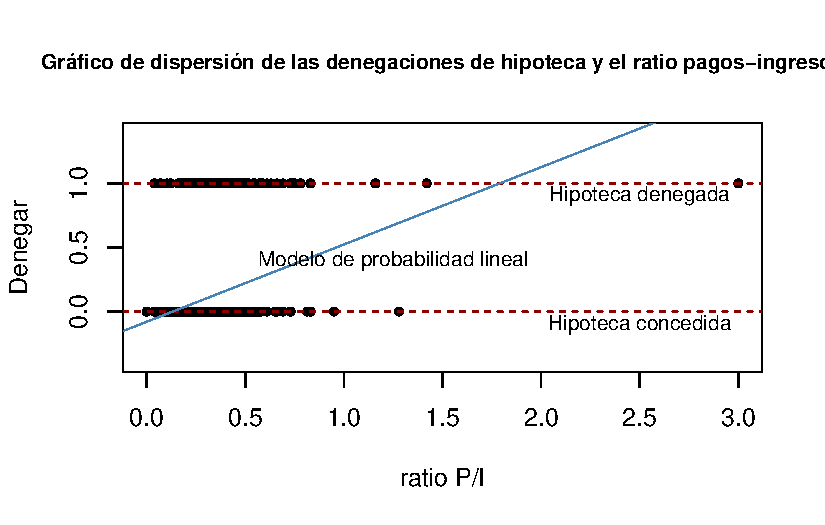
\includegraphics{cap1_files/figure-pdf/grafico-1.pdf}

Presentación de la regresión

\begin{Shaded}
\begin{Highlighting}[]
\FunctionTok{library}\NormalTok{(stargazer)}
\FunctionTok{library}\NormalTok{(sandwich)}
\NormalTok{eshr }\OtherTok{\textless{}{-}} \FunctionTok{list}\NormalTok{(}\FunctionTok{sqrt}\NormalTok{(}\FunctionTok{diag}\NormalTok{(}\FunctionTok{vcovHC}\NormalTok{(denymod1, }
                              \AttributeTok{type =} \StringTok{"HC1"}\NormalTok{))))}

\FunctionTok{stargazer}\NormalTok{(denymod1,denymod1, }
          \AttributeTok{type =} \StringTok{"text"}\NormalTok{, }
          \AttributeTok{se =}\NormalTok{ eshr)}
\end{Highlighting}
\end{Shaded}

\begin{verbatim}

============================================================
                                    Dependent variable:     
                                ----------------------------
                                            deny            
                                     (1)            (2)     
------------------------------------------------------------
pirat                              0.604***      0.604***   
                                   (0.098)        (0.061)   
                                                            
Constant                           -0.080**      -0.080***  
                                   (0.032)        (0.021)   
                                                            
------------------------------------------------------------
Observations                        2,380          2,380    
R2                                  0.040          0.040    
Adjusted R2                         0.039          0.039    
Residual Std. Error (df = 2378)     0.318          0.318    
F Statistic (df = 1; 2378)        98.406***      98.406***  
============================================================
Note:                            *p<0.1; **p<0.05; ***p<0.01
\end{verbatim}

Como los modelos de regresión lineal simple poseen el problema de sesgo
de variable omitida, y de debido a que el gráfico muestra
comportamientos que no son solo explicados por la variable independiente
(\emph{pirat}), se añade otra variable que puede ayudar a explicar el
fenómeno. La variable es respecto a la conseción de hipoteca a las
personas negras (\emph{afam})

\begin{Shaded}
\begin{Highlighting}[]
\FunctionTok{colnames}\NormalTok{(HMDA)[}\DecValTok{13}\NormalTok{] }\OtherTok{\textless{}{-}} \StringTok{"negra"}

\NormalTok{denymod2 }\OtherTok{\textless{}{-}} \FunctionTok{lm}\NormalTok{(deny }\SpecialCharTok{\textasciitilde{}} 
\NormalTok{                 pirat }\SpecialCharTok{+} 
\NormalTok{                 negra, }
               \AttributeTok{data =}\NormalTok{ HMDA)}

\NormalTok{eshr }\OtherTok{\textless{}{-}} \FunctionTok{list}\NormalTok{(}\FunctionTok{sqrt}\NormalTok{(}\FunctionTok{diag}\NormalTok{(}\FunctionTok{vcovHC}\NormalTok{(denymod1, }
                              \AttributeTok{type =} \StringTok{"HC1"}\NormalTok{))),}
             \FunctionTok{sqrt}\NormalTok{(}\FunctionTok{diag}\NormalTok{(}\FunctionTok{vcovHC}\NormalTok{(denymod2, }
                              \AttributeTok{type =} \StringTok{"HC1"}\NormalTok{))))}


\FunctionTok{stargazer}\NormalTok{(denymod1, }
\NormalTok{          denymod2,}
          \AttributeTok{type =} \StringTok{"text"}\NormalTok{,}
          \AttributeTok{se =}\NormalTok{ eshr,}
          \AttributeTok{df =}\NormalTok{ F, }
          \AttributeTok{report =} \StringTok{"vcts*"}\NormalTok{)}
\end{Highlighting}
\end{Shaded}

\begin{verbatim}

================================================
                        Dependent variable:     
                    ----------------------------
                                deny            
                         (1)            (2)     
------------------------------------------------
pirat                   0.604          0.597    
                      t = 6.128      t = 6.247  
                      (0.098)***    (0.096)***  
                                                
negrayes                               0.047    
                                     t = 3.387  
                                    (0.014)***  
                                                
Constant                -0.080        -0.096    
                      t = -2.500    t = -3.105  
                      (0.032)**     (0.031)***  
                                                
------------------------------------------------
Observations            2,380          2,380    
R2                      0.040          0.045    
Adjusted R2             0.039          0.044    
Residual Std. Error     0.318          0.318    
F Statistic           98.406***      55.614***  
================================================
Note:                *p<0.1; **p<0.05; ***p<0.01
\end{verbatim}

Miremos los valores ajustados

\(\widehat{y}_i\)

\begin{Shaded}
\begin{Highlighting}[]
\CommentTok{\# modelo con un solo regresor}
\FunctionTok{summary}\NormalTok{(denymod1}\SpecialCharTok{$}\NormalTok{fitted.values)}
\end{Highlighting}
\end{Shaded}

\begin{verbatim}
    Min.  1st Qu.   Median     Mean  3rd Qu.     Max. 
-0.07991  0.08908  0.11926  0.11975  0.14340  1.73070 
\end{verbatim}

\begin{Shaded}
\begin{Highlighting}[]
\CommentTok{\# modelo con dos regresores}

\FunctionTok{summary}\NormalTok{(denymod2}\SpecialCharTok{$}\NormalTok{fitted.values)}
\end{Highlighting}
\end{Shaded}

\begin{verbatim}
    Min.  1st Qu.   Median     Mean  3rd Qu.     Max. 
-0.09614  0.08800  0.11874  0.11975  0.14859  1.69459 
\end{verbatim}

\subsection{Porcentaje predicho
correctamente}\label{porcentaje-predicho-correctamente}

Mirada a los valores ajustados

\begin{Shaded}
\begin{Highlighting}[]
\NormalTok{denymod2}\SpecialCharTok{$}\NormalTok{fitted.values}
\end{Highlighting}
\end{Shaded}

\begin{verbatim}
            1             2             3             4             5 
 0.0357740938  0.1088880900  0.1259074499  0.0948681447  0.1187445298 
            6             7             8             9            10 
 0.0471153745  0.1596254083  0.0709917596  0.0888990484  0.0581507716 
           11            12            13            14            15 
 0.1178417344  0.1357490232  0.0709917596  0.1187445298  0.0113007969 
           16            17            18            19            20 
 0.1187445298  0.0411462782  0.0948681447  0.0888990484  0.1715636008 
           21            22            23            24            25 
 0.1247136260  0.1366518186  0.1417181195  0.1366518186  0.1476872157 
           26            27            28            29            30 
 0.1178417344  0.1715636008  0.1297799269  0.0888990484  0.1059035418 
           31            32            33            34            35 
 0.1655945046  0.1247136260  0.1596254083  0.1715636008  0.1068063372 
           36            37            38            39            40 
 0.1306827223  0.1664973000  0.1127754335  0.1306827223  0.1715636008 
           41            42            43            44            45 
 0.1247136260  0.1485900111  0.1127754335  0.1485900111  0.1536563120 
           46            47            48            49            50 
 0.0769608559  0.0650226633  0.1715636008  0.1068063372  0.1655945046 
           51            52            53            54            55 
 0.1536563120  0.0650226633  0.0462125791  0.1835017934  0.1187445298 
           56            57            58            59            60 
 0.0912866846  0.1068063372  0.1488810396  0.1476872157  0.1888739891 
           61            62            63            64            65 
 0.1080001610  0.1751450495  0.0954650452  0.0703948477  0.0930774204 
           66            67            68            69            70 
 0.0739763077  0.1217290779  0.1050156129  0.1596254083  0.1608192321 
           71            72            73            74            75 
 0.1127754335  0.1091939848  0.1178417344  0.1294888985  0.0578597432 
           76            77            78            79            80 
 0.0339833581  0.0411462782  0.0739763077  0.0620381152  0.1655945046 
           81            82            83            84            85 
 0.0662164871  0.1655945046  0.0888990484  0.1649976041  0.1408301905 
           86            87            88            89            90 
 0.1068063372  0.0345802700  0.1417181195  0.0948681447  0.1178417344 
           91            92            93            94            95 
 0.1354579948  0.0999344456  0.1068063372  0.1417181195  0.0900928722 
           96            97            98            99           100 
 0.1476872157  0.0948681447  0.1306827223  0.0948681447  0.0411462782 
          101           102           103           104           105 
 0.0650226633  0.1381366594  0.1596254083  0.1417181195  0.1175507060 
          106           107           108           109           110 
 0.1596254083  0.1068063372  0.1357490232  0.0769608559  0.2679719366 
          111           112           113           114           115 
 0.0608442914  0.1070973656  0.1187445298  0.2252854673  0.0859145003 
          116           117           118           119           120 
 0.1799203447  0.0614412033  0.1008372410  0.2312545636  0.0172698931 
          121           122           123           124           125 
 0.1297799269  0.1187445298  0.1476872157  0.0879962530  0.1485900111 
          126           127           128           129           130 
 0.1187445298  0.1485900111  0.1008372410  0.1238108307  0.1485900111 
          131           132           133           134           135 
 0.1008372410  0.0411462782  0.1366518186  0.1366518186  0.0650226633 
          136           137           138           139           140 
 0.1799203447  0.1787265209  0.1247136260  0.1447026676  0.1882770659 
          141           142           143           144           145 
 0.1864863415  0.1936492616  0.1303768388  0.1685790527  0.1094850019 
          146           147           148           149           150 
 0.0638288395  0.0644257514  0.1948430854  0.0877052246  0.1363459351 
          151           152           153           154           155 
 0.1187445298  0.1366518186  0.0948681447  0.0113007969  0.1068063372 
          156           157           158           159           160 
 0.1464933919  0.1798009601  0.1056125134  0.0715886715  0.1848746828 
          161           162           163           164           165 
 0.1205352541  0.0505774499  0.1319362271  0.0948681447  0.0745732196 
          166           167           168           169           170 
 0.1094850019  0.0918835965  0.1325853981  0.1524624882  0.1691759532 
          171           172           173           174           175 
 0.1253105266  0.1312796228  0.1596254083  0.1068063372  0.0621574998 
          176           177           178           179           180 
 0.1596254083  0.1835017934  0.1835017934  0.0829299521  0.0769608559 
          181           182           183           184           185 
 0.1127754335  0.1835017934  0.1655945046  0.1059035418  0.1655945046 
          186           187           188           189           190 
 0.0650226633  0.1638037802  0.0829299521  0.1366518186  0.0888990484 
          191           192           193           194           195 
 0.1605282037  0.1426209149  0.1536563120  0.1462023635  0.0411462782 
          196           197           198           199           200 
 0.3864510667  0.1775326971  0.1793234214  0.0948681447  0.0787515802 
          201           202           203           204           205 
 0.0941444263  0.0665075042  0.1261984669  0.1787265209  0.1774133125 
          206           207           208           209           210 
 0.1043590087  0.1836808590  0.1851731331  0.0709917596  0.0888990484 
          211           212           213           214           215 
 0.1799800257  0.1500748634  0.1238108307  0.1482244353  0.1518058840 
          216           217           218           219           220 
 0.1081792266  0.1313915857  0.0943309251  0.0508759001  0.0745732196 
          221           222           223           224           225 
 0.1118726381  0.1190355582  0.1443445136  0.1115816097  0.1273922907 
          226           227           228           229           230 
 0.0947487600  0.1895305706  0.0687831890  0.1610580014 -0.0222455235 
          231           232           233           234           235 
 0.1536563120  0.0301631402  0.0725437260  0.0763639440  0.0829299521 
          236           237           238           239           240 
 0.1187445298  0.0948681447  0.0948681447  0.0590535670  0.0590535670 
          241           242           243           244           245 
 0.1417181195  0.2014090822  0.1536563120  0.1247136260  0.1238108307 
          246           247           248           249           250 
 0.1596254083  0.1894708897  0.1655945046  0.1306827223  0.1247136260 
          251           252           253           254           255 
 0.1954399859  0.1417181195  0.1008372410  0.1008372410  0.1238108307 
          256           257           258           259           260 
 0.1715636008  0.1655945046  0.1247136260  0.1297799269  0.1068063372 
          261           262           263           264           265 
 0.1545591074  0.0232389894  0.0829299521  0.1306827223  0.1536563120 
          266           267           268           269           270 
 0.0769608559  0.0948681447  0.1187445298  0.1485900111  0.1417181195 
          271           272           273           274           275 
 0.1306827223  0.0700889642  0.1178417344  0.0530844708  0.0769608559 
          276           277           278           279           280 
 0.2431927561  0.1008372410  0.1724663962  0.1954399859  0.1127754335 
          281           282           283           284           285 
 0.1127754335 -0.0483901659  0.0999344456  0.1903736851  0.1187445298 
          286           287           288           289           290 
 0.0948681447  0.0650226633  0.1068063372  0.1476872157  0.0709917596 
          291           292           293           294           295 
 0.1068063372  0.1715636008  0.1297799269  0.1187445298  0.1158196626 
          296           297           298           299           300 
 0.0999344456 -0.0125755882  0.1664973000  0.1724663962  0.1247136260 
          301           302           303           304           305 
 0.1068063372  0.0652614326  0.0411462782  0.1536563120  0.1476872157 
          306           307           308           309           310 
 0.1745481490  0.1042396240  0.0697382548  0.1485900111  0.1204755732 
          311           312           313           314           315 
 0.0881827518  0.1223259784  0.1386738790  0.0681265961  0.1127754335 
          316           317           318           319           320 
 0.1492988745  0.0948681447  0.0615605879  0.1066272716  0.1066272716 
          321           322           323           324           325 
 0.1191026837  0.1287726133  0.0835268640  0.2730382375  0.1133723340 
          326           327           328           329           330 
 0.1829048929  0.1605282037  0.1605282037 -0.0066064920  0.1536563120 
          331           332           333           334           335 
 0.1357490232  0.1247136260  0.0888990484  0.0829299521 -0.0006373957 
          336           337           338           339           340 
 0.1187445298  0.1187445298  0.1426209149  0.1715636008  0.0709917596 
          341           342           343           344           345 
 0.1605282037  0.1187445298  0.0471153745  0.1844045888 -0.0015401911 
          346           347           348           349           350 
 0.0471153745  0.0351771819 -0.0125755882  0.0292080857 -0.0961429361 
          351           352           353           354           355 
 0.0761774451  0.1393379165  0.1297799269  0.1187445298  0.0709917596 
          356           357           358           359           360 
 0.0590535670  0.1178417344  0.0855563577  0.0910479267  0.0843028415 
          361           362           363           364           365 
 0.0229405391  0.0677087612  0.1405242957  0.1724663962  0.1168941017 
          366           367           368           369           370 
 0.1023220818  0.0943234919  0.0709917596  0.1994989732  0.1826661236 
          371           372           373           374           375 
 0.1072838759  0.1118726381  0.1127754335  0.1127754335  0.1417181195 
          376           377           378           379           380 
 0.1417181195  0.1715636008  0.1596254083  0.2133472748  0.1426209149 
          381           382           383           384           385 
 0.1238108307  0.1954399859  0.0530844708  0.1894708897  0.1605282037 
          386           387           388           389           390 
 0.1485900111  0.1963427813  0.1954399859  0.0590535670  0.1697728765 
          391           392           393           394           395 
 0.1835017934  0.1715636008  0.1476872157  0.0709917596  0.1655945046 
          396           397           398           399           400 
 0.1127754335  0.0948681447  0.1306827223  0.1127754335  0.1187445298 
          401           402           403           404           405 
 0.0530844708  0.2312545636  0.0113007969  0.1238108307  0.0530844708 
          406           407           408           409           410 
 0.0590535670  0.0769608559  0.1238108307  0.1118726381  0.1238108307 
          411           412           413           414           415 
 0.0292080857  0.4709212099  0.0530844708  0.0351771819  0.1247136260 
          416           417           418           419           420 
 0.1426209149  0.1238108307  0.1655945046  0.1417181195  0.1306827223 
          421           422           423           424           425 
 0.1247136260  0.1426209149  0.0939653493  0.1247136260  0.1596254083 
          426           427           428           429           430 
 0.1485900111  0.1485900111  0.1417181195  0.1068063372  0.1835017934 
          431           432           433           434           435 
 0.0465184626  0.1014341415  0.1626099564  0.1479334069  0.0491971272 
          436           437           438           439           440 
 0.0871083241  0.0441308264  0.0906897727  0.1094850019  0.0417431901 
          441           442           443           444           445 
 0.0853175884  0.1109847092  0.1602223088  0.0954650452  0.1312796228 
          446           447           448           449           450 
 0.2324483874  0.2043936303  0.0942712328 -0.0075689797  0.1074032377 
          451           452           453           454           455 
 0.1121785330  0.1056125134  0.1402332673  0.1835017934  0.1148571862 
          456           457           458           459           460 
 0.1360474735  0.2300607398  0.1358161488  0.0483091983  0.3169185078 
          461           462           463           464           465 
 0.2476770002  0.1152227621  0.2366267593  0.1163568822  0.1673852289 
          466           467           468           469           470 
 0.0614412033  0.0539723997  0.1217290779  0.1924554378  0.0542782946 
          471           472           473           474           475 
 0.0987406218  0.1840986939  0.1196324587  0.1321675632 -0.0627159975 
          476           477           478           479           480 
 0.1799203447  0.2993022702  0.1076942662  0.1015461043  0.0924805084 
          481           482           483           484           485 
 0.1644006808  0.1241167255  0.0832209805  0.1017251699  0.0136884331 
          486           487           488           489           490 
 0.1894708897  0.1536563120  0.1319884976  0.1485900111  0.0581507716 
          491           492           493           494           495 
 0.1426209149  0.1357490232  0.2202191664  0.1451802062  0.1849343865 
          496           497           498           499           500 
 0.0382214224  0.1316974578  0.1521640380  0.0462125791  0.1297799269 
          501           502           503           504           505 
 0.0103980015  0.0232389894 -0.0015401911  0.0103980015  0.0053317006 
          506           507           508           509           510 
 0.1238108307  0.1715636008  0.1655945046  0.0530844708  0.1187445298 
          511           512           513           514           515 
 0.1366518186  0.1775326971  0.1894708897  0.1655945046  0.1306827223 
          516           517           518           519           520 
 0.1476872157  0.1247136260  0.0351771819  0.0829299521  0.1655945046 
          521           522           523           524           525 
 0.1485900111  0.1596254083  0.1417181195  0.1485900111  0.0948681447 
          526           527           528           529           530 
 0.1426209149  0.1476872157  0.0709917596  0.1127754335  0.1426209149 
          531           532           533           534           535 
 0.0829299521  0.1596254083  0.0232389894  0.0769608559  0.1187445298 
          536           537           538           539           540 
 0.1536563120  0.0590535670  0.0709917596  0.1605282037  0.0650226633 
          541           542           543           544           545 
 0.1178417344  0.0650226633  0.1655945046  0.1127754335  0.1476872157 
          546           547           548           549           550 
 0.0948681447  0.0411462782  0.1247136260  0.1015535261  0.1604013972 
          551           552           553           554           555 
 0.1766447682  0.1142080266  0.1995586542  0.0346399624  0.0731928970 
          556           557           558           559           560 
 0.2259420715  0.1107459399  0.0928983434  0.1263849657  0.3452642933 
          561           562           563           564           565 
 0.1164762668  0.1273997239  0.0912866846  0.1798606410  0.1195801996 
          566           567           568           569           570 
 0.1097237598  0.0961216494  0.0418028825  0.1682806024  0.1584987100 
          571           572           573           574           575 
 0.0768414712  0.4367108464  0.1723992707  0.0807810738  0.1148646081 
          576           577           578           579           580 
 0.1112831594  0.2489827868  0.1272803393  0.1830316994  0.0129647147 
          581           582           583           584           585 
 0.0965394844  0.1257209396  0.1041799431  0.1525892947  0.0575612930 
          586           587           588           589           590 
 0.1173716404  0.1824944798  0.0327895457  0.0692010353  0.0650226633 
          591           592           593           594           595 
 0.0948681447  0.0999344456  0.2052964257  0.0948681447  0.1626099564 
          596           597           598           599           600 
 0.1357490232  0.1297799269  0.0641198679  0.0113007969 -0.0483901659 
          601           602           603           604           605 
 0.1187445298 -0.0125755882  0.1068063372  0.1068063372  0.0948681447 
          606           607           608           609           610 
 0.0172698931  0.0948681447  0.3864510667  0.2500646478  0.1297799269 
          611           612           613           614           615 
-0.0125755882  0.0590535670  0.1605282037  0.1844045888  0.0530844708 
          616           617           618           619           620 
 0.0829299521  0.0650226633  0.1187445298  0.0524875589  0.0327895457 
          621           622           623           624           625 
 0.5962722317  0.1187445298  0.0697979358  0.0948681447  0.0757670321 
          626           627           628           629           630 
 0.1921644094  0.0900928722  0.1279892026  0.1560439596  0.1199383536 
          631           632           633           634           635 
 0.0739763077  0.0966588690  0.1450085625  0.0924805084  0.1226170068 
          636           637           638           639           640 
 0.1175507060  0.0769608559  0.1127754335  0.1068063372  0.1187445298 
          641           642           643           644           645 
 0.0650226633  0.1724663962  0.0948681447  0.1476872157  0.1784354925 
          646           647           648           649           650 
 0.1596254083  0.1596254083  0.1366518186  0.1784354925  0.1306827223 
          651           652           653           654           655 
 0.0650226633  0.1306827223  0.0351771819  0.1775326971  0.1247136260 
          656           657           658           659           660 
 0.1247136260  0.0709917596  0.0999344456  0.0590535670  0.0650226633 
          661           662           663           664           665 
 0.1775326971  0.1127754335  0.0530844708  0.1306827223  0.1247136260 
          666           667           668           669           670 
 0.1118726381  0.0471153745  0.1187445298  0.0879962530  0.1008372410 
          671           672           673           674           675 
 0.0709917596  0.1476872157  0.1715636008  0.0948681447  0.1118726381 
          676           677           678           679           680 
 0.0709917596  0.1366518186  0.1306827223  0.1306827223  0.1775326971 
          681           682           683           684           685 
 0.0829299521  0.1366518186  0.1068063372  0.0172698931  0.1068063372 
          686           687           688           689           690 
 0.1476872157  0.0888990484  0.0769608559  0.0232389894  0.1724663962 
          691           692           693           694           695 
 0.0948681447  0.0232389894  0.0650226633  0.0283052903 -0.0066064920 
          696           697           698           699           700 
-0.0364519733  0.1306827223  0.0351771819  0.0351771819 -0.0185446845 
          701           702           703           704           705 
-0.0075092874  0.1655945046  0.1655945046  0.0509952848  0.0345802700 
          706           707           708           709           710 
 0.0906897727  0.1288919980  0.0229331059  0.0942712328  0.1169538054 
          711           712           713           714           715 
 0.1763388733  0.0787515802  0.1312796228  0.0897869773  0.1220201063 
          716           717           718           719           720 
 0.0500999226  0.0799454040  0.1384425429  0.1008372410  0.0817361283 
          721           722           723           724           725 
 0.1444116392  0.1342641710  0.1787265209  0.1139692573  0.1333613870 
          726           727           728           729           730 
 0.1426805958  0.0650226633  0.1805172453  0.0304019095  0.0083162487 
          731           732           733           734           735 
 0.1295411576  0.0578597432  0.0626350271  0.0957560736 -0.0036219438 
          736           737           738           739           740 
 0.0829299521  0.1420240144  0.0983824792  0.1396363667  0.1655945046 
          741           742           743           744           745 
 0.1605282037  0.1366518186  0.1008372410  0.1127754335  0.1008372410 
          746           747           748           749           750 
 0.1605282037  0.1238108307  0.0709917596  0.1894708897  0.1247136260 
          751           752           753           754           755 
 0.1008372410  0.0709917596  0.1187445298  0.2193163710  0.0829299521 
          756           757           758           759           760 
 0.1775326971  0.1238108307  0.1008372410  0.0292080857  0.0888990484 
          761           762           763           764           765 
 0.0641198679  0.1655945046  0.1127754335  0.1715636008  0.1536563120 
          766           767           768           769           770 
 0.1008372410  0.1357490232  0.1571183988  0.1545591074  0.1775326971 
          771           772           773           774           775 
 0.1596254083  0.1476872157  0.0471153745  0.1183789540  0.1417181195 
          776           777           778           779           780 
-0.0006373957  0.0530844708  0.1596254083  0.1775326971  0.1417181195 
          781           782           783           784           785 
 0.1596254083  0.1118726381  0.0530844708  0.0769608559  0.1125889347 
          786           787           788           789           790 
 0.1417181195  0.1357490232  0.1715636008  0.2969146226  0.1008372410 
          791           792           793           794           795 
 0.0462125791  0.1775326971  0.1068063372  0.1366518186  0.1724663962 
          796           797           798           799           800 
 0.2551309487  0.1605282037  0.1357490232  0.2252854673  0.0939653493 
          801           802           803           804           805 
 0.0351771819  0.0351771819  0.0581507716  0.3446673928  0.2560337441 
          806           807           808           809           810 
 0.1596254083  0.2611000449  0.1545591074  0.1485900111  0.1963427813 
          811           812           813           814           815 
 0.1784354925  0.0999344456  0.1835017934  0.1485900111  0.1059035418 
          816           817           818           819           820 
 0.1655945046  0.1835017934  0.1655945046  0.1017251699  0.4461420294 
          821           822           823           824           825 
 0.1068063372  0.0590535670  0.1178417344  0.1536563120  0.1715636008 
          826           827           828           829           830 
 0.0411462782  0.0888990484  0.1187445298  0.1485900111  0.1357490232 
          831           832           833           834           835 
 0.1664973000  0.1247136260  0.1366518186  0.1306827223  0.2193163710 
          836           837           838           839           840 
 0.1068063372  0.1536563120  0.1187445298  0.2261882627  0.1127754335 
          841           842           843           844           845 
 0.1008372410  0.1127754335  0.0888990484  0.0530844708  0.1247136260 
          846           847           848           849           850 
 0.0650226633  0.0650226633  0.1187445298  0.0292080857  0.1297799269 
          851           852           853           854           855 
 0.1068063372  0.0769608559  0.1894708897  0.0829299521  0.1059035418 
          856           857           858           859           860 
 0.0709917596  0.1366518186  0.0351771819  0.0715886715  0.1127754335 
          861           862           863           864           865 
 0.1199383536  0.1565214755  0.1211321774  0.0089131606  0.1271012737 
          866           867           868           869           870 
 0.1181476293  0.1202293706  0.1513283681  0.0560690189  0.1364056274 
          871           872           873           874           875 
 0.0984495933  0.1465530957  0.1306827223  0.0960619685  0.0924805084 
          876           877           878           879           880 
 0.0850117049  0.0841760350  0.0838178811  0.0515847635  0.2026029060 
          881           882           883           884           885 
 0.0985689780  0.0942712328  0.2133472748  0.1318765461  0.0853175884 
          886           887           888           889           890 
 0.1536563120  0.1429119433  0.1300858218  0.2918483217  0.1411212076 
          891           892           893           894           895 
 0.1470977371  0.1651169659  0.0206125838  0.1273922907  0.1638037802 
          896           897           898           899           900 
 0.1667883284  0.1333613870  0.1148571862  0.0873470820  0.1441057671 
          901           902           903           904           905 
 0.0399524544  0.1276384932  0.1444116392  0.1748540439  0.0697979358 
          906           907           908           909           910 
 0.0753491971  0.0626350271  0.1500748634  0.0545693116  0.1026279653 
          911           912           913           914           915 
 0.1026279653  0.1318765461  0.0017502405  0.0945622612  0.1279892026 
          916           917           918           919           920 
 0.1435088438  0.0769608559  0.1074032377  0.1978276336  0.0626350271 
          921           922           923           924           925 
 0.1055453992  0.1962831004  0.0626350271  0.0357740938  0.1448294741 
          926           927           928           929           930 
 0.0292080857  0.1321675632  0.1829048929  0.1276981742  0.1435088438 
          931           932           933           934           935 
 0.0942712328  0.0841237759  0.1664301744  0.0829299521  0.0286111738 
          936           937           938           939           940 
 0.1900677902  0.1008372410  0.0853175884 -0.0089941282  0.1715636008 
          941           942           943           944           945 
 0.0471153745  0.0292080857  0.0590535670  0.1775326971  0.0590535670 
          946           947           948           949           950 
 0.0113007969  0.0471153745  0.1178417344  0.0530844708  0.2193163710 
          951           952           953           954           955 
 0.1297799269  0.1068063372  0.1297799269  0.1178417344  0.1306827223 
          956           957           958           959           960 
 0.1068063372  0.1127754335  0.1476872157  0.1417181195  0.0820271567 
          961           962           963           964           965 
 0.1297799269  0.0590535670  0.1536563120  0.1178417344  0.1476872157 
          966           967           968           969           970 
 0.1426209149  0.0590535670  0.0232389894  0.1536563120  0.1008372410 
          971           972           973           974           975 
 0.1127754335  0.1655945046  0.1417181195  0.0948681447  0.0351771819 
          976           977           978           979           980 
 0.0709917596  0.0709917596  0.1357490232  0.1247136260  0.0948681447 
          981           982           983           984           985 
 0.1366518186  0.1366518186  0.0581507716  0.1775326971  0.1775326971 
          986           987           988           989           990 
 0.1059035418  0.1655945046  0.1118726381  0.0471153745  0.0530844708 
          991           992           993           994           995 
 0.1178417344  0.1366518186  0.1306827223 -0.0066064920  0.0411462782 
          996           997           998           999          1000 
 0.0232389894  0.0948681447  0.1127754335  0.2252854673  0.0292080857 
         1001          1002          1003          1004          1005 
 0.0888990484  0.1238108307  0.1357490232  0.1008372410  0.1008372410 
         1006          1007          1008          1009          1010 
 0.1605282037  0.1247136260  0.1536563120  0.2073781785  0.1655945046 
         1011          1012          1013          1014          1015 
 0.3694465733  0.1775326971  0.1247136260  0.1247136260  0.1545591074 
         1016          1017          1018          1019          1020 
 0.1008372410  0.1954399859  0.1306827223  0.1476872157  0.1835017934 
         1021          1022          1023          1024          1025 
 0.1118726381  0.3267601040  0.1605282037  0.1476872157  0.1775326971 
         1026          1027          1028          1029          1030 
 0.1247136260  0.0760580605  0.0760580605  0.0411462782  0.2909455263 
         1031          1032          1033          1034          1035 
 0.1118726381  0.1008372410  0.1844045888  0.1417181195  0.0769608559 
         1036          1037          1038          1039          1040 
 0.1844045888  0.2202191664  0.0888990484  0.1366518186  0.1187445298 
         1041          1042          1043          1044          1045 
 0.2014090822  0.1187445298  0.1596254083  0.1059035418  0.0351771819 
         1046          1047          1048          1049          1050 
-0.0125755882  0.0948681447  0.1178417344  0.1715636008  0.0709917596 
         1051          1052          1053          1054          1055 
 0.1238108307  0.0650226633  0.0999344456  0.0590535670  0.0829299521 
         1056          1057          1058          1059          1060 
 0.2023118776  0.1306827223  0.1426209149  0.1068063372  0.0948681447 
         1061          1062          1063          1064          1065 
 0.0590535670  0.0232389894  0.0769608559  0.1417181195  0.1835017934 
         1066          1067          1068          1069          1070 
 0.0641198679  0.1247136260  0.1485900111  0.1775326971  0.1008372410 
         1071          1072          1073          1074          1075 
 0.1590285078  0.1330703699  0.0888990484  0.1118726381  0.1402332673 
         1076          1077          1078          1079          1080 
 0.0590535670  0.1241167255  0.0888990484  0.1145661578  0.0686041234 
         1081          1082          1083          1084          1085 
 0.0888990484  0.1775326971  0.1247136260  0.1187445298  0.1127754335 
         1086          1087          1088          1089          1090 
 0.1655945046  0.1402332673  0.1655945046  0.1187445298  0.1118726381 
         1091          1092          1093          1094          1095 
 0.0888990484  0.1068063372  0.0769608559  0.1545591074  1.6945859460 
         1096          1097          1098          1099          1100 
 0.1476872157  0.1417181195  0.0829299521  0.0769608559  0.0709917596 
         1101          1102          1103          1104          1105 
 0.1247136260  0.1247136260  0.0641198679  0.1187445298  0.4461420294 
         1106          1107          1108          1109          1110 
 0.1238108307  0.1715636008  0.0292080857  0.0760580605  0.1238108307 
         1111          1112          1113          1114          1115 
 0.0760580605  0.2014090822  0.0351771819  0.0650226633  0.2073781785 
         1116          1117          1118          1119          1120 
 0.1247136260  0.1238108307  0.0053317006  0.1536563120 -0.0006373957 
         1121          1122          1123          1124          1125 
-0.0185446845  0.0888990484  0.0411462782  0.0700889642  0.0292080857 
         1126          1127          1128          1129          1130 
 0.0471153745  0.0351771819  0.0999344456  0.1536563120  0.1426209149 
         1131          1132          1133          1134          1135 
 0.0769608559  0.0769608559 -0.0125755882  0.1485900111  0.1715636008 
         1136          1137          1138          1139          1140 
 0.2073781785  0.0590535670  0.0879962530  0.0333864576  0.1715636008 
         1141          1142          1143          1144          1145 
 0.1020310648  0.1297799269  0.1253105266  0.1127754335  0.0521816754 
         1146          1147          1148          1149          1150 
 0.0601280062  0.0345802700  0.1115816097  0.1187445298  0.1605282037 
         1151          1152          1153          1154          1155 
 0.0650226633  0.1187445298  0.0650226633  0.1357490232  0.1127754335 
         1156          1157          1158          1159          1160 
 0.1655945046  0.0590535670  0.1187445298  0.0948681447  0.0709917596 
         1161          1162          1163          1164          1165 
 0.1536563120  0.0999344456  0.1127754335  0.0223361940  0.1008372410 
         1166          1167          1168          1169          1170 
 0.0590535670  0.0700889642  0.1357490232  0.0700889642  0.1247136260 
         1171          1172          1173          1174          1175 
 0.1357490232  0.1775326971  0.0769608559  0.1127754335  0.1894708897 
         1176          1177          1178          1179          1180 
 0.1068063372  0.1008372410  0.0888990484  0.1954399859  0.0471153745 
         1181          1182          1183          1184          1185 
 0.0939653493  0.1306827223  0.1476872157  0.0948681447  0.1247136260 
         1186          1187          1188          1189          1190 
 0.1306827223  0.1357490232  0.1357490232  0.1127754335  0.0888990484 
         1191          1192          1193          1194          1195 
 0.0939653493  0.1127754335  0.1715636008  0.0829299521  0.1357490232 
         1196          1197          1198          1199          1200 
 0.0053317006  0.1247136260  0.0471153745  0.1596254083  0.1596254083 
         1201          1202          1203          1204          1205 
 0.1417181195  0.1008372410  0.1127754335  0.1835017934  0.1178417344 
         1206          1207          1208          1209          1210 
 0.1426209149  0.2312545636  0.1775326971  0.1835017934  0.0948681447 
         1211          1212          1213          1214          1215 
 0.1247136260  0.1963427813  0.0053317006  0.1008372410  0.1008372410 
         1216          1217          1218          1219          1220 
 0.1118726381  0.1417181195  0.1127754335  0.1008372410  0.0769608559 
         1221          1222          1223          1224          1225 
 0.1417181195  0.1715636008  0.1059035418  0.1596254083  0.0590535670 
         1226          1227          1228          1229          1230 
 0.0888990484  0.1596254083  0.2790073338  0.0888990484  0.0471153745 
         1231          1232          1233          1234          1235 
 0.1536563120  0.0829299521  0.1008372410  0.1715636008  0.0530844708 
         1236          1237          1238          1239          1240 
 0.0769608559  0.1417181195  0.1187445298  0.0939653493 -0.0364519733 
         1241          1242          1243          1244          1245 
 0.1068063372  0.2073781785  0.1835017934  0.1357490232  0.1715636008 
         1246          1247          1248          1249          1250 
 0.0888990484  0.1715636008  0.0471153745  0.1247136260  0.1596254083 
         1251          1252          1253          1254          1255 
 0.0769608559  0.0769608559 -0.0543592622  0.1187445298  0.0530844708 
         1256          1257          1258          1259          1260 
 0.0292080857 -0.0185446845  0.1536563120  0.1366518186  0.1297799269 
         1261          1262          1263          1264          1265 
 0.0769608559  0.0053317006  0.1247136260  0.1664973000  0.1247136260 
         1266          1267          1268          1269          1270 
 0.0530844708  0.1059035418  0.3983892592  0.0551662235  0.0113007969 
         1271          1272          1273          1274          1275 
 0.1127754335  0.1154540981  0.1178417344  0.1008372410  0.0581507716 
         1276          1277          1278          1279          1280 
 0.2372236599  0.0172698931  0.1894708897  0.2321573590  0.1835017934 
         1281          1282          1283          1284          1285 
 0.3169185078  0.1462023635  0.1966338097  0.0829299521  0.1115816097 
         1286          1287          1288          1289          1290 
 0.1447026676  0.1181476293  0.0829299521  0.0632319390  0.1476872157 
         1291          1292          1293          1294          1295 
 0.0859145003  0.1417181195  0.1247136260  0.0495030107  0.0972557923 
         1296          1297          1298          1299          1300 
 0.1127754335  0.1306827223  0.0939653493  0.0900928722  0.0948681447 
         1301          1302          1303          1304          1305 
 0.1655945046  0.0089131606  0.1357490232  0.0650226633  0.1297799269 
         1306          1307          1308          1309          1310 
 0.1485900111  0.0172698931  0.0232389894  0.1894708897  0.1417181195 
         1311          1312          1313          1314          1315 
 0.1127754335  0.1715636008  0.1127754335  0.1008372410 -0.0066064920 
         1316          1317          1318          1319          1320 
 0.1068063372  0.1118726381  0.1068063372  0.0829299521  0.1417181195 
         1321          1322          1323          1324          1325 
 0.6679013869  0.1178417344  0.0471153745  0.0939653493  0.1306827223 
         1326          1327          1328          1329          1330 
 0.0948681447  0.1596254083  0.0999344456  0.2133472748 -0.0245137808 
         1331          1332          1333          1334          1335 
 0.0760580605  0.0471153745  0.1187445298  0.1417181195  0.1545591074 
         1336          1337          1338          1339          1340 
 0.1715636008  0.1476872157  0.0650226633  0.1297799269  0.2372236599 
         1341          1342          1343          1344          1345 
 0.0172698931  0.0172698931  0.0888990484  0.1187445298  0.0292080857 
         1346          1347          1348          1349          1350 
 0.1008372410  0.1655945046  0.1715636008  0.1127754335  0.2014090822 
         1351          1352          1353          1354          1355 
 0.1068063372  0.0471153745  0.1775326971  0.1306827223  0.0113007969 
         1356          1357          1358          1359          1360 
 0.1068063372  0.1476872157  0.0530844708  0.1306827223  0.1127754335 
         1361          1362          1363          1364          1365 
 0.1775326971  0.1715636008  0.1306827223  0.1187445298  0.1068063372 
         1366          1367          1368          1369          1370 
 0.1187445298  0.0411462782  0.1297799269  0.0769608559  0.1366518186 
         1371          1372          1373          1374          1375 
 0.1187445298  0.1178417344  0.1306827223  0.0590535670  0.1664973000 
         1376          1377          1378          1379          1380 
 0.1068063372  0.1068063372  0.1306827223  0.1306827223  0.1596254083 
         1381          1382          1383          1384          1385 
-0.0006373957  0.0888990484  0.1187445298  0.1357490232  0.2193163710 
         1386          1387          1388          1389          1390 
 0.1835017934  0.0700889642  0.0471153745  0.1724663962  0.3148219114 
         1391          1392          1393          1394          1395 
 0.1118726381  0.2321573590  0.1417181195  0.0521816754  0.1844045888 
         1396          1397          1398          1399          1400 
-0.0125755882  0.1775326971  0.0888990484  0.2202191664  0.1059035418 
         1401          1402          1403          1404          1405 
 0.0232389894  0.1476872157  0.0700889642  0.2142500702  0.1476872157 
         1406          1407          1408          1409          1410 
 0.0641198679  0.0793484921  0.1256015550  0.1518655877  0.0238359013 
         1411          1412          1413          1414          1415 
 0.1082911781  0.1176626574  0.2133472748  0.0634110046  0.1954399859 
         1416          1417          1418          1419          1420 
 0.0736181651  0.1297799269  0.1118726381  0.1492988745  0.0872873897 
         1421          1422          1423          1424          1425 
 0.1223856821  0.2128100552  0.0223361940  0.1187445298  0.1485900111 
         1426          1427          1428          1429          1430 
 0.1476872157  0.1306827223  0.1417181195  0.1417181195  0.1685790527 
         1431          1432          1433          1434          1435 
 0.0709917596  0.1127754335  0.0417431901  0.0888990484 -0.0280952408 
         1436          1437          1438          1439          1440 
 0.0829299521  0.1220201063  0.1605282037  0.1127754335  0.1476872157 
         1441          1442          1443          1444          1445 
 0.1545591074  0.2491618524  0.1894708897  0.1775326971  0.1476872157 
         1446          1447          1448          1449          1450 
 0.0820271567  0.1306827223  0.1306827223  0.1306827223  0.1775326971 
         1451          1452          1453          1454          1455 
 0.1306827223  0.1306827223  0.1306827223  0.1306827223  0.1306827223 
         1456          1457          1458          1459          1460 
 0.0411462782  0.0590535670 -0.0066064920  0.0053317006  0.0709917596 
         1461          1462          1463          1464          1465 
 0.1297799269  0.1297799269  0.0521816754  0.1775326971  0.1247136260 
         1466          1467          1468          1469          1470 
 0.1596254083  0.2482739235  0.1715636008  0.1229229017  0.1945520570 
         1471          1472          1473          1474          1475 
 0.1420240144  0.1199383536  0.1545591074  0.1611251042  0.1187445298 
         1476          1477          1478          1479          1480 
 0.1715636008  0.1536563120  0.1297799269  0.1775326971  0.1306827223 
         1481          1482          1483          1484          1485 
 0.1417181195  0.0530844708  0.1118726381  0.1894708897  0.1187445298 
         1486          1487          1488          1489          1490 
 0.0948681447  0.1775326971  0.0650226633  0.0829299521  0.1476872157 
         1491          1492          1493          1494          1495 
 0.0709917596  0.0769608559  0.0948681447  0.0888990484  0.1835017934 
         1496          1497          1498          1499          1500 
 0.0951069140  0.1228631980  0.1485303302  0.0590535670  0.1835017934 
         1501          1502          1503          1504          1505 
 0.0140988405  0.0948681447  0.1187445298  0.1306827223  0.0709917596 
         1506          1507          1508          1509          1510 
 0.1306827223  0.1357490232  0.1596254083 -0.0006373957  0.1476872157 
         1511          1512          1513          1514          1515 
 0.1835017934  0.0590535670  0.1187445298  0.1068063372  0.1187445298 
         1516          1517          1518          1519          1520 
 0.1476872157  0.1187445298  0.1247136260  0.0351771819  0.1068063372 
         1521          1522          1523          1524          1525 
 0.1068063372  0.1426209149 -0.0364519733  0.1894708897  0.0709917596 
         1526          1527          1528          1529          1530 
 0.1187445298  0.1835017934  0.0820271567  0.1655945046  0.1068063372 
         1531          1532          1533          1534          1535 
 0.1417181195  0.1366518186  0.1357490232  0.1247136260  0.1545591074 
         1536          1537          1538          1539          1540 
 0.0650226633  0.1715636008  0.1417181195  0.1238108307  0.1247136260 
         1541          1542          1543          1544          1545 
 0.1655945046  0.1187445298  0.1008372410  0.1238108307  0.0590535670 
         1546          1547          1548          1549          1550 
 0.0769608559  0.0948681447  0.0292080857  0.1417181195  0.0769608559 
         1551          1552          1553          1554          1555 
 0.1655945046  0.1187445298  0.0820271567  0.0530844708  0.1596254083 
         1556          1557          1558          1559          1560 
 0.1059035418  0.1476872157  0.0888990484  0.1068063372  0.0829299521 
         1561          1562          1563          1564          1565 
 0.1008372410  0.1366518186  0.1655945046  0.0709917596  0.1059035418 
         1566          1567          1568          1569          1570 
 0.1596254083  0.0769608559  0.1068063372  0.0829299521  0.0999344456 
         1571          1572          1573          1574          1575 
 0.0709917596  0.1655945046  0.1596254083  0.0888990484  0.0590535670 
         1576          1577          1578          1579          1580 
 0.0650226633  0.0948681447  0.1357490232  0.1306827223  0.0650226633 
         1581          1582          1583          1584          1585 
 0.0650226633  0.0879962530  0.1008372410  0.1297799269  0.1247136260 
         1586          1587          1588          1589          1590 
 0.1596254083  0.0829299521  0.3625746816  0.0471153745  0.0530844708 
         1591          1592          1593          1594          1595 
 0.1118726381  0.1238108307  0.1068063372  0.1008372410  0.2491618524 
         1596          1597          1598          1599          1600 
 0.2014090822  0.0948681447  0.1664973000  0.1775326971  0.1536563120 
         1601          1602          1603          1604          1605 
 0.0829299521  0.1835017934  0.0709917596  0.1417181195  0.1485900111 
         1606          1607          1608          1609          1610 
 0.1844045888  0.1596254083  0.0948681447  0.0769608559  0.1417181195 
         1611          1612          1613          1614          1615 
 0.0999344456  0.1068063372  0.1655945046  0.1476872157  0.0999344456 
         1616          1617          1618          1619          1620 
 0.0999344456  0.0650226633  0.0999344456  0.0411462782  0.0641198679 
         1621          1622          1623          1624          1625 
 0.0530844708  0.1059035418  0.0113007969  0.1068063372  0.1655945046 
         1626          1627          1628          1629          1630 
 0.1059035418  0.1775326971  0.1426209149  0.1297799269  0.0351771819 
         1631          1632          1633          1634          1635 
 0.0172698931  0.1835017934  0.1118726381  0.1655945046  0.0650226633 
         1636          1637          1638          1639          1640 
 0.1476872157  0.1417181195  0.1426209149  0.1187445298  0.0888990484 
         1641          1642          1643          1644          1645 
-0.0364519733  0.1118726381  0.1118726381  0.1715636008  0.1366518186 
         1646          1647          1648          1649          1650 
 0.0948681447  0.1306827223  0.1247136260  0.1536563120  0.1366518186 
         1651          1652          1653          1654          1655 
 0.0888990484  0.1127754335  0.0829299521  0.1118726381  0.0530844708 
         1656          1657          1658          1659          1660 
 0.1247136260  0.1068063372  0.1187445298  0.1476872157  0.1306827223 
         1661          1662          1663          1664          1665 
 0.1357490232  0.1297799269  0.1178417344  0.0888990484  0.0888990484 
         1666          1667          1668          1669          1670 
 0.1775326971  0.1068063372  0.1118726381  0.1178417344  0.0939653493 
         1671          1672          1673          1674          1675 
 0.1178417344  0.1357490232  0.0760580605  0.1536563120  0.0700889642 
         1676          1677          1678          1679          1680 
 0.1417181195  0.1426209149  0.1178417344  0.0888990484  0.0888990484 
         1681          1682          1683          1684          1685 
 0.1596254083  0.1247136260  0.0948681447  0.1068063372  0.1068063372 
         1686          1687          1688          1689          1690 
 0.1008372410  0.0351771819  0.1715636008  0.1963427813  0.1655945046 
         1691          1692          1693          1694          1695 
 0.1187445298  0.1536563120  0.1476872157  0.1178417344  0.1476872157 
         1696          1697          1698          1699          1700 
 0.1476872157  0.1187445298  0.1127754335  0.1715636008  0.0948681447 
         1701          1702          1703          1704          1705 
 0.1238108307  0.0650226633  0.1366518186  0.2014090822  0.1357490232 
         1706          1707          1708          1709          1710 
 0.1596254083  0.0769608559  0.0769608559  0.0709917596  0.1008372410 
         1711          1712          1713          1714          1715 
 0.2073781785  0.0888990484  0.1059035418  0.1068063372  0.1963427813 
         1716          1717          1718          1719          1720 
 0.1297799269  0.1476872157  0.1357490232  0.2193163710  0.0411462782 
         1721          1722          1723          1724          1725 
-0.0304828771  0.1715636008  0.0939653493  0.0172698931  0.1059035418 
         1726          1727          1728          1729          1730 
 0.1008372410  0.0650226633  0.0709917596  0.1247136260  0.0709917596 
         1731          1732          1733          1734          1735 
 0.2014090822  0.1366518186  0.0590535670  0.1008372410  0.1187445298 
         1736          1737          1738          1739          1740 
 0.1476872157  0.1844045888  0.2909455263  0.1655945046  0.1596254083 
         1741          1742          1743          1744          1745 
 0.0700889642 -0.0304828771  0.1247136260  0.0462125791  0.1297799269 
         1746          1747          1748          1749          1750 
 0.1127754335  0.1417181195  0.1008372410 -0.0185446845  0.0888990484 
         1751          1752          1753          1754          1755 
 0.0650226633  0.2849764300  0.1357490232  0.1357490232  0.1536563120 
         1756          1757          1758          1759          1760 
 0.0709917596  0.1247136260  0.1357490232  0.1417181195  0.1476872157 
         1761          1762          1763          1764          1765 
 0.0530844708  0.1844045888  0.0590535670  0.0948681447  0.1835017934 
         1766          1767          1768          1769          1770 
 0.1417181195  0.0530844708 -0.0304828771  0.1118726381  0.1357490232 
         1771          1772          1773          1774          1775 
 0.1655945046  0.0471153745  0.1655945046  0.1366518186  0.1596254083 
         1776          1777          1778          1779          1780 
 0.1476872157  0.1536563120  0.2551309487  0.0829299521  0.0471153745 
         1781          1782          1783          1784          1785 
 0.1297799269  0.1596254083  0.0879962530  0.0879962530  0.1187445298 
         1786          1787          1788          1789          1790 
 0.0709917596  0.1476872157  0.0888990484 -0.0254165762  0.1127754335 
         1791          1792          1793          1794          1795 
 0.0820271567  0.0590535670  0.0769608559  0.1357490232  0.1417181195 
         1796          1797          1798          1799          1800 
 0.1775326971  0.1068063372  0.1068063372  0.1238108307  0.1357490232 
         1801          1802          1803          1804          1805 
 0.0351771819  0.1536563120  0.1357490232  0.0888990484  0.0411462782 
         1806          1807          1808          1809          1810 
 0.1844045888  0.2014090822  0.1366518186  0.2014090822  0.1835017934 
         1811          1812          1813          1814          1815 
 0.1476872157  0.1178417344  0.2142500702 -0.0543592622  0.2133472748 
         1816          1817          1818          1819          1820 
 0.1187445298  0.2014090822  0.2133472748  0.1784354925  0.1844045888 
         1821          1822          1823          1824          1825 
 0.1306827223  0.1903736851  0.0709917596  0.1247136260  0.1596254083 
         1826          1827          1828          1829          1830 
 0.1426209149  0.1655945046  0.1068063372  0.1724663962  0.1426209149 
         1831          1832          1833          1834          1835 
 0.1306827223  0.0113007969  0.1306827223  0.1715636008  0.0462125791 
         1836          1837          1838          1839          1840 
 0.1715636008  0.0232389894  0.1417181195  0.1417181195  0.1655945046 
         1841          1842          1843          1844          1845 
 0.1068063372  0.1536563120  0.1187445298  0.0172698931  0.1536563120 
         1846          1847          1848          1849          1850 
 0.0879962530 -0.0125755882  0.1127754335  0.1008372410  0.0581507716 
         1851          1852          1853          1854          1855 
 0.1059035418  0.1068063372  0.1059035418  0.1059035418  0.0351771819 
         1856          1857          1858          1859          1860 
 0.0769608559  0.1238108307  0.0709917596  0.0530844708  0.1357490232 
         1861          1862          1863          1864          1865 
 0.1655945046  0.0471153745  0.1068063372  0.1247136260  0.1068063372 
         1866          1867          1868          1869          1870 
 0.0709917596  0.1187445298  0.1187445298  0.1127754335  0.0471153745 
         1871          1872          1873          1874          1875 
 0.1306827223  0.1127754335  0.1426209149  0.1426209149  0.1187445298 
         1876          1877          1878          1879          1880 
 0.1306827223  0.1426209149  0.1664973000  0.1485900111  0.1247136260 
         1881          1882          1883          1884          1885 
 0.1008372410  0.1366518186  0.1417181195  0.1306827223  0.0760580605 
         1886          1887          1888          1889          1890 
 0.2133472748  0.0172698931  0.1366518186  0.1426209149  0.1664973000 
         1891          1892          1893          1894          1895 
 0.1536563120  0.1655945046  0.0650226633  0.1366518186  0.1187445298 
         1896          1897          1898          1899          1900 
 0.1715636008  0.1187445298  0.1605282037  0.1366518186  0.1008372410 
         1901          1902          1903          1904          1905 
 0.2073781785  0.1068063372  0.0700889642  0.1178417344  0.2014090822 
         1906          1907          1908          1909          1910 
 0.1835017934  0.3924201630  0.0650226633  0.0939653493  0.1247136260 
         1911          1912          1913          1914          1915 
 0.2073781785  0.1536563120  0.2969146226  0.1426209149  0.1545591074 
         1916          1917          1918          1919          1920 
 0.2014090822  0.1247136260  0.1366518186  0.1835017934  0.1178417344 
         1921          1922          1923          1924          1925 
 0.1536563120  0.0530844708  0.1127754335  0.1008372410  0.1247136260 
         1926          1927          1928          1929          1930 
 0.0590535670  0.0471153745  0.7983187096  0.7983187096  0.1366518186 
         1931          1932          1933          1934          1935 
 0.1545591074  0.1485900111  0.1247136260  0.1059035418  0.1247136260 
         1936          1937          1938          1939          1940 
 0.2073781785  0.1894708897  0.2312545636  0.1187445298  0.1536563120 
         1941          1942          1943          1944          1945 
 0.0769608559  0.1835017934  0.0888990484  0.1426209149  0.1366518186 
         1946          1947          1948          1949          1950 
 0.1485900111  0.1775326971  0.1008372410  0.1835017934  0.0769608559 
         1951          1952          1953          1954          1955 
 0.1187445298  0.1187445298  0.1844045888  0.1536563120  0.1187445298 
         1956          1957          1958          1959          1960 
 0.1536563120  0.1775326971  0.1306827223  0.1426209149  0.2312545636 
         1961          1962          1963          1964          1965 
 0.1127754335  0.1485900111  0.1775326971  0.1306827223  0.0769608559 
         1966          1967          1968          1969          1970 
 0.1187445298  0.1835017934  0.1954399859  0.3267601040  0.1059035418 
         1971          1972          1973          1974          1975 
 0.0709917596  0.1357490232  0.0411462782  0.1545591074  0.1238108307 
         1976          1977          1978          1979          1980 
 0.0948681447  0.1596254083  0.1605282037  0.1485900111  0.1247136260 
         1981          1982          1983          1984          1985 
 0.1366518186  0.2252854673  0.1306827223  0.1008372410  0.1068063372 
         1986          1987          1988          1989          1990 
 0.0650226633  0.1187445298  0.1247136260  0.0530844708  0.1127754335 
         1991          1992          1993          1994          1995 
 0.0590535670  0.1068063372  0.1014341415  0.1276981742  0.0905629662 
         1996          1997          1998          1999          2000 
 0.1846956172  0.1118800600  0.0596504789  0.1429119433  0.0333864576 
         2001          2002          2003          2004          2005 
-0.0209323208  0.0906897727  0.0972557923  0.1312796228  0.1127754335 
         2006          2007          2008          2009          2010 
 0.0098010896  0.0814302448  0.1342641710  0.1199383536  0.0811392278 
         2011          2012          2013          2014          2015 
 0.1420240144  0.0751701315  0.1163568822  0.1109847092  0.1327644751 
         2016          2017          2018          2019          2020 
 0.0805423159  0.1265043504  0.0915777131  0.1032248886  0.1363459351 
         2021          2022          2023          2024          2025 
-0.0107848582  0.0787515802  0.0659105922  0.1624905718  0.1074032377 
         2026          2027          2028          2029          2030 
 0.1253105266  0.1536563120  0.1469709306  0.1139692573  0.1387932637 
         2031          2032          2033          2034          2035 
 0.1125366642  0.1566408602  0.1303768388  0.1050156129  0.1363459351 
         2036          2037          2038          2039          2040 
 0.1761598077  0.0954650452  0.1176104097  0.0990465166  0.1211321774 
         2041          2042          2043          2044          2045 
 0.0918239042  0.2145410986  0.1644006808  0.0972557923  0.1799203447 
         2046          2047          2048          2049          2050 
 0.1817110691  0.1195801996  0.1044186896  0.1579540686  0.0820271567 
         2051          2052          2053          2054          2055 
 0.0931967936  0.2599062211  0.1350327266  0.1005387907  0.0996434171 
         2056          2057          2058          2059          2060 
 0.1655945046  0.0912866846  0.1354579948  0.1721605014  0.1097908854 
         2061          2062          2063          2064          2065 
 0.1715636008  0.0965991881  0.1229229017  0.0817361283  0.1223259784 
         2066          2067          2068          2069          2070 
 0.0763639440  0.1253105266  0.0948681447  0.0883021365  0.1151630811 
         2071          2072          2073          2074          2075 
 0.1360549181  0.1345551994  0.1632068570  0.0930774204  0.0721855834 
         2076          2077          2078          2079          2080 
 0.0805423159  0.1235198022  0.1187445298  0.1267953788  0.1271535214 
         2081          2082          2083          2084          2085 
 0.1193414303  0.0703948477  0.0787515802  0.1262655811  0.0694994855 
         2086          2087          2088          2089          2090 
 0.1265640541  0.0136884331  0.0952262987  0.1217290779  0.1247136260 
         2091          2092          2093          2094          2095 
 0.0942712328  0.0868098624  0.1512686644  0.1211321774  0.0841237759 
         2096          2097          2098          2099          2100 
 0.1612370670  0.1513954937 -0.0030250319  0.0703948477  0.1870832420 
         2101          2102          2103          2104          2105 
 0.1287129096  0.1074032377  0.0434071023  0.1223259784  0.1715636008 
         2106          2107          2108          2109          2110 
 0.1638037802  0.1166479106  0.1057916018  0.0823330402  0.0894959603 
         2111          2112          2113          2114          2115 
 0.1336672705  0.1649976041  0.0978526928  0.1109847092  0.1441057671 
         2116          2117          2118          2119          2120 
 0.0811392278  0.0083759410  0.1239376372  0.0971364076  0.0892571910 
         2121          2122          2123          2124          2125 
 0.1159987510  0.0894959603  0.1211321774  0.1524624882  0.1047171626 
         2126          2127          2128          2129          2130 
 0.0381617301  0.0972557923  0.1439266787  0.0999344456  0.1655945046 
         2131          2132          2133          2134          2135 
 0.1127754335  0.1127754335  0.1596254083  0.1031592190  0.0834074794 
         2136          2137          2138          2139          2140 
 0.1315706513  0.1102684240  0.1414270911  0.0049138657  0.1072838759 
         2141          2142          2143          2144          2145 
 0.1210127927  0.0188815519  0.0099279074  0.1187445298  0.1420165697 
         2146          2147          2148          2149          2150 
 0.1664973000  0.1250643354  0.1396363667  0.1247136260  0.1664973000 
         2151          2152          2153          2154          2155 
 0.1715636008  0.1261387746  0.1693027825  0.1596254083  0.1649976041 
         2156          2157          2158          2159          2160 
 0.1835017934  0.1068063372  0.1388006969  0.0888990484  0.1307349814 
         2161          2162          2163          2164          2165 
 0.1589762487  0.1136111033  0.1366518186  0.1123575986  0.1260865155 
         2166          2167          2168          2169          2170 
 0.1040008547  0.1357564450  0.1550963270  0.0733793958  0.1151630811 
         2171          2172          2173          2174          2175 
 0.1890604766  0.1484706265  0.0198962987  0.1811215904  0.1546710475 
         2176          2177          2178          2179          2180 
 0.1403452301  0.1347342764  0.1618339675  0.1857700563  0.1379650271 
         2181          2182          2183          2184          2185 
 0.0235374397  0.2368655059  0.1366443854 -0.0283936911  0.0942115404 
         2186          2187          2188          2189          2190 
 0.1137901689  0.0496223954  0.0939130902  0.0654330650  0.1554544810 
         2191          2192          2193          2194          2195 
 0.1063885023 -0.0317363875  0.1106191334  0.1176700906  0.1703697770 
         2196          2197          2198          2199          2200 
 0.1022026971  0.0800647887  0.0788112725  0.1290636304  0.1523431036 
         2201          2202          2203          2204          2205 
 0.1239376372  0.1900081092  0.1127754335  0.1838002436  0.1895902743 
         2206          2207          2208          2209          2210 
 0.1398154323  0.1205352541  0.1229229017  0.1512089835  0.0953382387 
         2211          2212          2213          2214          2215 
 0.0516518890  0.1369502689  0.0961813531  0.1427328549  0.2053486848 
         2216          2217          2218          2219          2220 
 0.1353908806  0.1051349976  0.1059035418  0.1177297943  0.1142677076 
         2221          2222          2223          2224          2225 
 0.1196921510  0.0952859796  0.1614235772  0.1421359544  0.1414793502 
         2226          2227          2228          2229          2230 
 0.1423821456  0.0955247489  0.1799203447  0.0641198679 -0.0254165762 
         2231          2232          2233          2234          2235 
 0.1575959147  0.1927613327  0.1469112269  0.0749313622  0.0923611238 
         2236          2237          2238          2239          2240 
 0.1540218878  0.1762791924  0.2133472748  0.1429716242  0.1266834387 
         2241          2242          2243          2244          2245 
 0.0781546797  0.0847803688  0.0871680050  0.0948681447  0.1019116801 
         2246          2247          2248          2249          2250 
 0.1060303483  0.0945100021  0.0779756027  0.1005387907  0.1324734467 
         2251          2252          2253          2254          2255 
 0.0555914917  0.1393304832  0.1262655811  0.1645797691  0.1008372410 
         2256          2257          2258          2259          2260 
 0.1775923781  0.1398080105  0.1337866551  0.1568199258  0.0809601508 
         2261          2262          2263          2264          2265 
 0.0684847387  0.1431581344  0.1629681104  0.1310931240  0.0342818198 
         2266          2267          2268          2269          2270 
 0.0608442914  0.0966588690  0.1161181356  0.0877052246  0.1154540981 
         2271          2272          2273          2274          2275 
 0.1220872319  0.1022101304  0.1223185566  0.0603667641  0.1613564517 
         2276          2277          2278          2279          2280 
 0.1148049271  0.1303768388  0.1263252848  0.1596254083  0.1596254083 
         2281          2282          2283          2284          2285 
 0.0053317006  0.0521816754  0.0829299521  0.1068063372  0.2491618524 
         2286          2287          2288          2289          2290 
 0.0760580605  0.1187445298  0.0172698931  0.0948681447  0.1127754335 
         2291          2292          2293          2294          2295 
 0.0760580605  0.0709917596  0.0829299521  0.1187445298  0.0650226633 
         2296          2297          2298          2299          2300 
 0.1306827223  0.1536563120  0.1118726381  0.1247136260  0.0848997534 
         2301          2302          2303          2304          2305 
 0.0820942823  0.1248330107  0.1217290779  0.1223259784  0.1476872157 
         2306          2307          2308          2309          2310 
 0.1894708897  0.0650226633  0.0769608559  0.0888990484  0.1775326971 
         2311          2312          2313          2314          2315 
 0.1715636008  0.1775326971  0.1536563120  0.2014090822  0.0948681447 
         2316          2317          2318          2319          2320 
 0.1342641710  0.1578346840  0.0495030107  0.0411462782  0.1068063372 
         2321          2322          2323          2324          2325 
 0.1127754335  0.1769357966  0.1835017934  0.2014090822  0.0590535670 
         2326          2327          2328          2329          2330 
 0.1605282037  0.1068063372  0.0232389894  0.1187445298  0.0948681447 
         2331          2332          2333          2334          2335 
 0.1596254083  0.1844045888  0.1366518186  0.1068063372  0.1306827223 
         2336          2337          2338          2339          2340 
 0.1703697770  0.0829299521  0.1372487191  0.0829299521  0.1954399859 
         2341          2342          2343          2344          2345 
 0.1068063372  0.1059035418  0.1127754335 -0.0424210696  0.0590535670 
         2346          2347          2348          2349          2350 
 0.1664973000  0.1596254083  0.1366518186  0.0888990484  0.1426209149 
         2351          2352          2353          2354          2355 
 0.1485900111  0.0471153745  0.1008372410  0.1247136260  0.1127754335 
         2356          2357          2358          2359          2360 
 0.1545591074  0.1008372410  0.1068063372  0.1187445298  0.1417181195 
         2361          2362          2363          2364          2365 
 0.1417181195  0.0650226633  0.1008372410  0.1306827223  0.1187445298 
         2366          2367          2368          2369          2370 
 0.0939653493  0.0948681447  0.1775326971  0.1306827223  0.0999344456 
         2371          2372          2373          2374          2375 
 0.1417181195  0.1357490232  0.1008372410  0.1596254083  0.1008372410 
         2376          2377          2378          2379          2380 
 0.0888990484  0.1297799269  0.0590535670  0.1417181195  0.1596254083 
\end{verbatim}

\begin{Shaded}
\begin{Highlighting}[]
\CommentTok{\# Porcentaje predicho correctamente}
\NormalTok{ppc }\OtherTok{\textless{}{-}}\FunctionTok{data.frame}\NormalTok{(denymod2}\SpecialCharTok{$}\NormalTok{model}\SpecialCharTok{$}\NormalTok{deny, denymod2}\SpecialCharTok{$}\NormalTok{fitted.values) }
\FunctionTok{head}\NormalTok{(ppc)}
\end{Highlighting}
\end{Shaded}

\begin{verbatim}
  denymod2.model.deny denymod2.fitted.values
1                   0             0.03577409
2                   0             0.10888809
3                   0             0.12590745
4                   0             0.09486814
5                   0             0.11874453
6                   0             0.04711537
\end{verbatim}

\begin{Shaded}
\begin{Highlighting}[]
\CommentTok{\# Cambiar de nombre}

\FunctionTok{names}\NormalTok{(ppc) }\OtherTok{\textless{}{-}} \FunctionTok{c}\NormalTok{(}\StringTok{"deny"}\NormalTok{, }\StringTok{"VA"}\NormalTok{)}
\FunctionTok{head}\NormalTok{(ppc)}
\end{Highlighting}
\end{Shaded}

\begin{verbatim}
  deny         VA
1    0 0.03577409
2    0 0.10888809
3    0 0.12590745
4    0 0.09486814
5    0 0.11874453
6    0 0.04711537
\end{verbatim}

\begin{Shaded}
\begin{Highlighting}[]
\CommentTok{\# Creando la variable y virgulilla}

\NormalTok{ppc}\SpecialCharTok{$}\NormalTok{y.c }\OtherTok{\textless{}{-}} \FunctionTok{ifelse}\NormalTok{(ppc}\SpecialCharTok{$}\NormalTok{VA}\SpecialCharTok{\textgreater{}}\FloatTok{0.5}\NormalTok{,}\DecValTok{1}\NormalTok{,}\DecValTok{0}\NormalTok{)}

\FunctionTok{head}\NormalTok{(ppc)}
\end{Highlighting}
\end{Shaded}

\begin{verbatim}
  deny         VA y.c
1    0 0.03577409   0
2    0 0.10888809   0
3    0 0.12590745   0
4    0 0.09486814   0
5    0 0.11874453   0
6    0 0.04711537   0
\end{verbatim}

\begin{Shaded}
\begin{Highlighting}[]
\FunctionTok{tail}\NormalTok{(ppc)}
\end{Highlighting}
\end{Shaded}

\begin{verbatim}
     deny         VA y.c
2375    0 0.10083724   0
2376    0 0.08889905   0
2377    0 0.12977993   0
2378    0 0.05905357   0
2379    1 0.14171812   0
2380    1 0.15962541   0
\end{verbatim}

\begin{Shaded}
\begin{Highlighting}[]
\CommentTok{\# Creando la variable PPC}

\NormalTok{ppc}\SpecialCharTok{$}\NormalTok{ppc }\OtherTok{\textless{}{-}} \FunctionTok{ifelse}\NormalTok{(ppc}\SpecialCharTok{$}\NormalTok{deny}\SpecialCharTok{==}\NormalTok{ppc}\SpecialCharTok{$}\NormalTok{y.c,}\DecValTok{1}\NormalTok{,}\DecValTok{0}\NormalTok{)}
\FunctionTok{head}\NormalTok{(ppc)}
\end{Highlighting}
\end{Shaded}

\begin{verbatim}
  deny         VA y.c ppc
1    0 0.03577409   0   1
2    0 0.10888809   0   1
3    0 0.12590745   0   1
4    0 0.09486814   0   1
5    0 0.11874453   0   1
6    0 0.04711537   0   1
\end{verbatim}

\begin{Shaded}
\begin{Highlighting}[]
\CommentTok{\# Calculando el PPC}

\FunctionTok{prop.table}\NormalTok{(}\FunctionTok{table}\NormalTok{(ppc}\SpecialCharTok{$}\NormalTok{ppc))}\SpecialCharTok{*}\DecValTok{100}
\end{Highlighting}
\end{Shaded}

\begin{verbatim}

       0        1 
11.84874 88.15126 
\end{verbatim}

\section{Ejemplo 2: Determinantes del trabajo femenino (Wooldridge
2009)}\label{ejemplo-2-determinantes-del-trabajo-femenino-wooldridge2009}

\begin{itemize}
\item
  \(y\): \textbf{inlf}: (la fuerza de trabajo femenino), una variable
  binaria que indica, si una mujer casada participó en la fuerza de
  trabajo durante 1975: \(infl=1\) la mujer informa haber trabajado
  fuera de la casa, por un salario ese año, cero otro caso
\item
  \(x_1=nwifeinc\) los ingreso del esposo en miles de dólares (-)
\item
  \(x_2=educ\) años de educación (+)
\item
  \(x_3=exper\) años de experiencia (+)
\item
  \(x_4=exper^2\) años de experiencia al cuadrado (-)
\item
  \(x_5=edad\) en años (-)
\item
  \(x_6=kidslt6\) hijo \textless{} 6 años (-)
\item
  \(x_7=kidsge6\) hijos entres 6 y 18 años (+)
\end{itemize}

\begin{Shaded}
\begin{Highlighting}[]
\FunctionTok{data}\NormalTok{(}\StringTok{"mroz"}\NormalTok{, }\AttributeTok{package =} \StringTok{"wooldridge"}\NormalTok{)}
\FunctionTok{str}\NormalTok{(mroz)}
\end{Highlighting}
\end{Shaded}

\begin{verbatim}
'data.frame':   753 obs. of  22 variables:
 $ inlf    : int  1 1 1 1 1 1 1 1 1 1 ...
 $ hours   : int  1610 1656 1980 456 1568 2032 1440 1020 1458 1600 ...
 $ kidslt6 : int  1 0 1 0 1 0 0 0 0 0 ...
 $ kidsge6 : int  0 2 3 3 2 0 2 0 2 2 ...
 $ age     : int  32 30 35 34 31 54 37 54 48 39 ...
 $ educ    : int  12 12 12 12 14 12 16 12 12 12 ...
 $ wage    : num  3.35 1.39 4.55 1.1 4.59 ...
 $ repwage : num  2.65 2.65 4.04 3.25 3.6 ...
 $ hushrs  : int  2708 2310 3072 1920 2000 1040 2670 4120 1995 2100 ...
 $ husage  : int  34 30 40 53 32 57 37 53 52 43 ...
 $ huseduc : int  12 9 12 10 12 11 12 8 4 12 ...
 $ huswage : num  4.03 8.44 3.58 3.54 10 ...
 $ faminc  : num  16310 21800 21040 7300 27300 ...
 $ mtr     : num  0.721 0.661 0.692 0.781 0.622 ...
 $ motheduc: int  12 7 12 7 12 14 14 3 7 7 ...
 $ fatheduc: int  7 7 7 7 14 7 7 3 7 7 ...
 $ unem    : num  5 11 5 5 9.5 7.5 5 5 3 5 ...
 $ city    : int  0 1 0 0 1 1 0 0 0 0 ...
 $ exper   : int  14 5 15 6 7 33 11 35 24 21 ...
 $ nwifeinc: num  10.9 19.5 12 6.8 20.1 ...
 $ lwage   : num  1.2102 0.3285 1.5141 0.0921 1.5243 ...
 $ expersq : int  196 25 225 36 49 1089 121 1225 576 441 ...
 - attr(*, "time.stamp")= chr "25 Jun 2011 23:03"
\end{verbatim}

\begin{Shaded}
\begin{Highlighting}[]
\CommentTok{\# Correr el modelo y crear el objeto}
\NormalTok{mroz.mpl }\OtherTok{\textless{}{-}} \FunctionTok{lm}\NormalTok{(inlf}\SpecialCharTok{\textasciitilde{}}
\NormalTok{                 nwifeinc}\SpecialCharTok{+}
\NormalTok{                 educ}\SpecialCharTok{+}
\NormalTok{                 exper}\SpecialCharTok{+}
                 \FunctionTok{I}\NormalTok{(exper}\SpecialCharTok{\^{}}\DecValTok{2}\NormalTok{)}\SpecialCharTok{+}
\NormalTok{                 age}\SpecialCharTok{+}
\NormalTok{                 kidslt6}\SpecialCharTok{+}
\NormalTok{                 kidsge6,}
               \AttributeTok{data =}\NormalTok{ mroz)}


\CommentTok{\# usando stargazer}
\FunctionTok{library}\NormalTok{(stargazer)}

\FunctionTok{stargazer}\NormalTok{(mroz.mpl,}
          \AttributeTok{type =} \StringTok{"text"}\NormalTok{, }
          \AttributeTok{digits =} \DecValTok{5}\NormalTok{)}
\end{Highlighting}
\end{Shaded}

\begin{verbatim}

===============================================
                        Dependent variable:    
                    ---------------------------
                               inlf            
-----------------------------------------------
nwifeinc                    -0.00341**         
                             (0.00145)         
                                               
educ                        0.03800***         
                             (0.00738)         
                                               
exper                       0.03949***         
                             (0.00567)         
                                               
I(exper2)                   -0.00060***        
                             (0.00018)         
                                               
age                         -0.01609***        
                             (0.00248)         
                                               
kidslt6                     -0.26181***        
                             (0.03351)         
                                               
kidsge6                       0.01301          
                             (0.01320)         
                                               
Constant                    0.58552***         
                             (0.15418)         
                                               
-----------------------------------------------
Observations                    753            
R2                            0.26422          
Adjusted R2                   0.25730          
Residual Std. Error     0.42713 (df = 745)     
F Statistic          38.21795*** (df = 7; 745) 
===============================================
Note:               *p<0.1; **p<0.05; ***p<0.01
\end{verbatim}

\begin{Shaded}
\begin{Highlighting}[]
\CommentTok{\# Punto de inflexión}
\FunctionTok{abs}\NormalTok{((}\FunctionTok{coefficients}\NormalTok{(mroz.mpl)[}\DecValTok{4}\NormalTok{])}\SpecialCharTok{/}\NormalTok{(}\FunctionTok{coefficients}\NormalTok{(mroz.mpl)[}\DecValTok{5}\NormalTok{]}\SpecialCharTok{*}\DecValTok{2}\NormalTok{))}
\end{Highlighting}
\end{Shaded}

\begin{verbatim}
   exper 
33.11387 
\end{verbatim}

\begin{Shaded}
\begin{Highlighting}[]
\CommentTok{\# Probar la multicolinealidad aproximada}
\FunctionTok{library}\NormalTok{(car)}

\FunctionTok{mean}\NormalTok{(}\FunctionTok{vif}\NormalTok{(mroz.mpl))}
\end{Highlighting}
\end{Shaded}

\begin{verbatim}
[1] 3.417547
\end{verbatim}

\begin{Shaded}
\begin{Highlighting}[]
\CommentTok{\# Normalidad de los errores}

\FunctionTok{library}\NormalTok{(tseries)}
\FunctionTok{jarque.bera.test}\NormalTok{(mroz.mpl}\SpecialCharTok{$}\NormalTok{residuals)}
\end{Highlighting}
\end{Shaded}

\begin{verbatim}

    Jarque Bera Test

data:  mroz.mpl$residuals
X-squared = 36.741, df = 2, p-value = 1.051e-08
\end{verbatim}

\[
H_0: u\sim N(\mu, \sigma^2)
\]

\subsection{El porcentaje predicho
correctamente}\label{el-porcentaje-predicho-correctamente}

Es una medida de bondad de ajuste

\begin{Shaded}
\begin{Highlighting}[]
\NormalTok{PPC.DTF }\OtherTok{\textless{}{-}} \FunctionTok{data.frame}\NormalTok{(mroz}\SpecialCharTok{$}\NormalTok{inlf, mroz.mpl}\SpecialCharTok{$}\NormalTok{fitted.values)}
\FunctionTok{names}\NormalTok{(PPC.DTF) }\OtherTok{\textless{}{-}} \FunctionTok{c}\NormalTok{(}\StringTok{"infl"}\NormalTok{, }\StringTok{"VA.infl"}\NormalTok{)}
\NormalTok{PPC.DTF}\SpecialCharTok{$}\NormalTok{ajuste }\OtherTok{\textless{}{-}} \FunctionTok{ifelse}\NormalTok{(mroz.mpl}\SpecialCharTok{$}\NormalTok{fitted.values}\SpecialCharTok{\textgreater{}=}\FloatTok{0.5}\NormalTok{,}\DecValTok{1}\NormalTok{,}\DecValTok{0}\NormalTok{)}
\NormalTok{PPC.DTF}\SpecialCharTok{$}\NormalTok{PPC }\OtherTok{\textless{}{-}} \FunctionTok{ifelse}\NormalTok{(PPC.DTF}\SpecialCharTok{$}\NormalTok{infl}\SpecialCharTok{==}\NormalTok{PPC.DTF}\SpecialCharTok{$}\NormalTok{ajuste,}\DecValTok{1}\NormalTok{,}\DecValTok{0}\NormalTok{)}
\FunctionTok{prop.table}\NormalTok{(}\FunctionTok{table}\NormalTok{(PPC.DTF}\SpecialCharTok{$}\NormalTok{PPC))}\SpecialCharTok{*}\DecValTok{100}
\end{Highlighting}
\end{Shaded}

\begin{verbatim}

       0        1 
26.56042 73.43958 
\end{verbatim}

\subsection{Interpretaciones ceteris
paribus}\label{interpretaciones-ceteris-paribus}

\begin{itemize}
\item
  Para interpretar las estimaciones, hay que recordar que una variación
  en la variable independiente modifica la probabilidad de que
  \(inlf=1\). Por ejemplo, \emph{educ} si las demás variables permanecen
  constantes, una año más de educación hace que la probabilidad de
  participación en la fuerza laboral aumente en 3.8\%. Si consideramos
  de forma literal a esta ecuación, entonces 10 años más educación
  incrementarían la probabilidad de permanecer en la fuerza laboral en
  38\%.
\item
  El coeficiente de \textbf{nwifeinc} significa que si
  \(\Delta nwifeinc=10\) (un incremento de \$10,000), la probabilidad de
  que una mujer permanecer en la fuerza de trabajo disminuye en 3.4\%.
  Como se puede ver, esta disminución es pequeña a pesar de aumentar el
  salario en 10,000 dólares.
\item
  La experiencia ha sido introducida como una función cuadrática para
  que el efecto de la experiencia sea decreciente sobre la probabilidad
  de participar en la fuerza laboral. \emph{Ceteris paribus}, la
  variación de la probabilidad se aproxima como
  \(0.039-2(0.0006)exper=0.039-0.0012exper\). El punto en el que la
  experiencia transcurrida no tiene efecto sobre la probabilidad de
  participación en la fuerza laboral es: \(0.039/0.0012=32.5\). Sólo 13
  mujeres de las 753 en esta muestra tiene más de 32 años de
  experiencia.
\end{itemize}

\begin{Shaded}
\begin{Highlighting}[]
\NormalTok{mroz}\SpecialCharTok{$}\NormalTok{dico.exper }\OtherTok{\textless{}{-}} \FunctionTok{ifelse}\NormalTok{(mroz}\SpecialCharTok{$}\NormalTok{exper}\SpecialCharTok{\textgreater{}}\FloatTok{32.5}\NormalTok{,}\DecValTok{1}\NormalTok{,}\DecValTok{0}\NormalTok{)}
\FunctionTok{table}\NormalTok{(mroz}\SpecialCharTok{$}\NormalTok{dico.exper)}
\end{Highlighting}
\end{Shaded}

\begin{verbatim}

  0   1 
740  13 
\end{verbatim}

\begin{itemize}
\tightlist
\item
  A diferencia de la cantidad de hijos entre 6 y 18 años, la cantidad de
  hijos menores a 6 años tiene un impacto enorme sobre la probabilidad
  de participación en la fuerza de trabajo. A tal punto que, tener un
  hijo menor a seis años adicional, reduce la probabilidad de
  participación en la fuerza trabajo en 26.18\%. En la muestra, menos de
  20\% de las mujeres tienen al menos un hijo pequeño.
\end{itemize}

\begin{Shaded}
\begin{Highlighting}[]
\NormalTok{mroz}\SpecialCharTok{$}\NormalTok{dic.hijo }\OtherTok{\textless{}{-}} \FunctionTok{ifelse}\NormalTok{(mroz}\SpecialCharTok{$}\NormalTok{kidslt6}\SpecialCharTok{\textgreater{}=}\DecValTok{1}\NormalTok{,}\DecValTok{1}\NormalTok{,}\DecValTok{0}\NormalTok{)}
\FunctionTok{prop.table}\NormalTok{(}\FunctionTok{table}\NormalTok{(mroz}\SpecialCharTok{$}\NormalTok{dic.hijo))}\SpecialCharTok{*}\DecValTok{100}
\end{Highlighting}
\end{Shaded}

\begin{verbatim}

       0        1 
80.47809 19.52191 
\end{verbatim}

\begin{itemize}
\tightlist
\item
  Respecto al PPC el modelo predice en 73.44\% a la variable
  \textbf{infl}.
\end{itemize}

\subsection{Límites del MPL}\label{luxedmites-del-mpl}

\begin{itemize}
\tightlist
\item
  Las dos desventajas más importantes son que las probabilidades
  ajustadas pueden ser menores que cero o mayores que uno.
\end{itemize}

\begin{Shaded}
\begin{Highlighting}[]
\FunctionTok{summary}\NormalTok{(mroz.mpl}\SpecialCharTok{$}\NormalTok{fitted.values)}
\end{Highlighting}
\end{Shaded}

\begin{verbatim}
   Min. 1st Qu.  Median    Mean 3rd Qu.    Max. 
-0.3451  0.4016  0.5880  0.5684  0.7592  1.1272 
\end{verbatim}

Se demuestra para este ejemplo que algunos valores ajustados son menores
que cero y mayores que uno.

\begin{itemize}
\tightlist
\item
  y, el efecto parcial de cualquier variable explicativa (si aparece en
  la ecuación en su nivel) es constante
\end{itemize}

\section{Ejemplo 3: Un modelo de probabilidad lineal para arrestos
(Wooldridge
2009)}\label{ejemplo-3-un-modelo-de-probabilidad-lineal-para-arrestos-wooldridge2009}

Sea \textbf{arr86} una variable binaria igual a uno si un hombre fue
arrestado en 1986 e igual a cero si no fue así. La población es un grupo
de hombres de California nacidos en 1960 o en 1961, que habían sido
detenidos al menos una vez antes de 1986. Un modelo de probabilidad
lineal para describir \textbf{arr86} es:

\[arr86=\beta_0+\beta_1pcnv+\beta_2avgsen+\beta_3tottime+\beta_4ptime86+\beta_5qemp86+u\]
donde:

\begin{itemize}
\item
  \(pcnv=\) proporción de arrestos previos que condujeron a una condena
  (+)
\item
  \(avgsen=\) sentencia promedio cumplida en condenas previas (en meses)
  (-)
\item
  \(tottime=\) meses en prisión y desde los 18 años de edad anteriores a
  1986 (-)
\item
  \(ptime86=\) meses en prisión en 1986 (+ -)
\item
  \(qemp86=\) cantidad de trimestres (0 a 4) que el hombre estuvo
  empleado legalmente en 1986.(-)
\end{itemize}

\begin{Shaded}
\begin{Highlighting}[]
\FunctionTok{data}\NormalTok{(}\StringTok{"crime1"}\NormalTok{, }\AttributeTok{package =} \StringTok{"wooldridge"}\NormalTok{)}
\FunctionTok{str}\NormalTok{(crime1)}
\end{Highlighting}
\end{Shaded}

\begin{verbatim}
'data.frame':   2725 obs. of  16 variables:
 $ narr86 : int  0 2 1 2 1 0 2 5 0 0 ...
 $ nfarr86: int  0 2 1 2 1 0 2 3 0 0 ...
 $ nparr86: int  0 0 0 1 0 0 1 5 0 0 ...
 $ pcnv   : num  0.38 0.44 0.33 0.25 0 ...
 $ avgsen : num  17.6 0 22.8 0 0 ...
 $ tottime: num  35.2 0 22.8 0 0 ...
 $ ptime86: int  12 0 0 5 0 0 0 0 9 0 ...
 $ qemp86 : num  0 1 0 2 2 4 0 0 0 3 ...
 $ inc86  : num  0 0.8 0 8.8 8.1 ...
 $ durat  : num  0 0 11 0 1 ...
 $ black  : int  0 0 1 0 0 0 1 0 1 0 ...
 $ hispan : int  0 1 0 1 0 0 0 0 0 1 ...
 $ born60 : int  1 0 1 1 0 1 1 1 1 1 ...
 $ pcnvsq : num  0.1444 0.1936 0.1089 0.0625 0 ...
 $ pt86sq : int  144 0 0 25 0 0 0 0 81 0 ...
 $ inc86sq: num  0 0.64 0 77.44 65.61 ...
 - attr(*, "time.stamp")= chr "25 Jun 2011 23:03"
\end{verbatim}

\begin{Shaded}
\begin{Highlighting}[]
\CommentTok{\# Creando la variable y}
\FunctionTok{table}\NormalTok{(crime1}\SpecialCharTok{$}\NormalTok{narr86)}
\end{Highlighting}
\end{Shaded}

\begin{verbatim}

   0    1    2    3    4    5    6    7    9   10   12 
1970  559  121   42   12   13    4    1    1    1    1 
\end{verbatim}

\begin{Shaded}
\begin{Highlighting}[]
\NormalTok{crime1}\SpecialCharTok{$}\NormalTok{arr86 }\OtherTok{\textless{}{-}} \FunctionTok{ifelse}\NormalTok{(crime1}\SpecialCharTok{$}\NormalTok{narr86}\SpecialCharTok{\textgreater{}}\DecValTok{0}\NormalTok{,}\DecValTok{1}\NormalTok{,}\DecValTok{0}\NormalTok{)}

\NormalTok{arr86.MPL }\OtherTok{\textless{}{-}} \FunctionTok{lm}\NormalTok{(arr86}\SpecialCharTok{\textasciitilde{}}
\NormalTok{                  pcnv}\SpecialCharTok{+}
\NormalTok{                  avgsen}\SpecialCharTok{+}
\NormalTok{                  tottime}\SpecialCharTok{+}
\NormalTok{                  ptime86}\SpecialCharTok{+}
\NormalTok{                  qemp86,}
                \AttributeTok{data =}\NormalTok{ crime1)}
\FunctionTok{stargazer}\NormalTok{(arr86.MPL, }
          \AttributeTok{digits =} \DecValTok{5}\NormalTok{,}
          \AttributeTok{type =} \StringTok{"text"}\NormalTok{)}
\end{Highlighting}
\end{Shaded}

\begin{verbatim}

===============================================
                        Dependent variable:    
                    ---------------------------
                               arr86           
-----------------------------------------------
pcnv                        -0.16244***        
                             (0.02124)         
                                               
avgsen                        0.00611          
                             (0.00645)         
                                               
tottime                      -0.00226          
                             (0.00498)         
                                               
ptime86                     -0.02197***        
                             (0.00463)         
                                               
qemp86                      -0.04283***        
                             (0.00540)         
                                               
Constant                    0.44062***         
                             (0.01723)         
                                               
-----------------------------------------------
Observations                   2,725           
R2                            0.04735          
Adjusted R2                   0.04560          
Residual Std. Error     0.43731 (df = 2719)    
F Statistic         27.02966*** (df = 5; 2719) 
===============================================
Note:               *p<0.1; **p<0.05; ***p<0.01
\end{verbatim}

\subsection{Porcentaje predicho
correctamente}\label{porcentaje-predicho-correctamente-1}

\begin{Shaded}
\begin{Highlighting}[]
\NormalTok{PPC.arr }\OtherTok{\textless{}{-}} \FunctionTok{data.frame}\NormalTok{(crime1}\SpecialCharTok{$}\NormalTok{arr86, arr86.MPL}\SpecialCharTok{$}\NormalTok{fitted.values)}
\FunctionTok{names}\NormalTok{(PPC.arr)}\OtherTok{\textless{}{-}} \FunctionTok{c}\NormalTok{(}\StringTok{"arr86"}\NormalTok{, }\StringTok{"valores\_ajustados"}\NormalTok{)}
\NormalTok{PPC.arr}\SpecialCharTok{$}\NormalTok{ajuste }\OtherTok{\textless{}{-}} \FunctionTok{ifelse}\NormalTok{(PPC.arr}\SpecialCharTok{$}\NormalTok{valores\_ajustados}\SpecialCharTok{\textgreater{}=}\FloatTok{0.5}\NormalTok{,}\DecValTok{1}\NormalTok{,}\DecValTok{0}\NormalTok{)}
\NormalTok{PPC.arr}\SpecialCharTok{$}\NormalTok{PPC }\OtherTok{\textless{}{-}}\FunctionTok{ifelse}\NormalTok{(PPC.arr}\SpecialCharTok{$}\NormalTok{arr86}\SpecialCharTok{==}\NormalTok{PPC.arr}\SpecialCharTok{$}\NormalTok{ajuste,}\DecValTok{1}\NormalTok{,}\DecValTok{0}\NormalTok{)}
\FunctionTok{prop.table}\NormalTok{(}\FunctionTok{table}\NormalTok{(PPC.arr}\SpecialCharTok{$}\NormalTok{PPC))}\SpecialCharTok{*}\DecValTok{100}
\end{Highlighting}
\end{Shaded}

\begin{verbatim}

       0        1 
27.70642 72.29358 
\end{verbatim}

\subsection{Interpretaciones}\label{interpretaciones}

\begin{itemize}
\item
  \(\widehat{\beta}_0=0.44062\), es la probabilidad de ser arrestado que
  se predice a un hombre, que no ha sido condenado, que no ha estado en
  prisión despues de los 18 años, que no ha estado en prisión en 1986 y
  que ha estado desempleado todo el año
\item
  \(\widehat{\beta}_2; \widehat{\beta}_3\) que pertenecen a las
  variables \emph{avgsen} y \emph{tottime}, respectivamente. No son
  estadísticamente significativas (no tiene asteriscos). El signo de
  \emph{avgsen} es contrauntuitivo, pues se esperaria que condenas más
  largas disminuyan la probabilidad de ser arrestado en 1986.Con
  respecto a \emph{tottime}, según los datos haber tenido meses en
  prisión de los 18 y antes de 1986, disminuye la probabilidad de ser
  arrestado en 1986.
\item
  \textbf{ptimes86} el aumento de probabilidad de ser condenado en 1986,
  disminuye la probabilidad de ser arrestado en promedio en 2.2\%. Si un
  hombre esta en prisión no puede ser arrestado. Como \textbf{ptimes86}
  esta medida en mese, 6 meses más en prisión, reduce la probabilidad de
  ser detenido en \(0.0022\times6\approx0.132\). En esta variable se
  puede observar otra vez, que el MPL no cierto en todos los rangos de
  variables independientes. Por ejemplo, si un hombre está en prisión
  durante 12 meses de 1986, no puede ser detenido en 1986.
  \textbf{Ceteris paribus}, cuando \(ptimr86=12\) la probabilidad
  predicha es de \(0.44-0.22\times12=0.177\) que es distinta de cero
\item
  \textbf{qemp86} tener un empleo reduce la probabilidad de detención de
  manera significativa. \textbf{Ceteris paribus} un hombre que ha sido
  empleado durante 4 trimestres, la probabilidad de ser detenido se
  reduce en \(0.04283\times\approx0.172\)
\end{itemize}

\section{Incorporando regresores binarios al
MPL}\label{incorporando-regresores-binarios-al-mpl}

En los modelos de variable dependiente binaria, se puede incluir
variables independientes binarias. Este coeficiente mide la diferencia
que se predice para la probabilidad en la relación con el grupo base.
Así, incluimos regresores binarios en el MPL para \textbf{arr86}

\begin{Shaded}
\begin{Highlighting}[]
\NormalTok{arr86.MPL.bi }\OtherTok{\textless{}{-}} \FunctionTok{lm}\NormalTok{(arr86}\SpecialCharTok{\textasciitilde{}}
\NormalTok{                  pcnv}\SpecialCharTok{+}
\NormalTok{                  avgsen}\SpecialCharTok{+}
\NormalTok{                  tottime}\SpecialCharTok{+}
\NormalTok{                  ptime86}\SpecialCharTok{+}
\NormalTok{                  qemp86}\SpecialCharTok{+}
\NormalTok{                    black}\SpecialCharTok{+}
\NormalTok{                    hispan,}
                \AttributeTok{data =}\NormalTok{ crime1)}

\FunctionTok{stargazer}\NormalTok{(arr86.MPL.bi, }
          \AttributeTok{digits =} \DecValTok{5}\NormalTok{,}
          \AttributeTok{type =} \StringTok{"text"}\NormalTok{)}
\end{Highlighting}
\end{Shaded}

\begin{verbatim}

===============================================
                        Dependent variable:    
                    ---------------------------
                               arr86           
-----------------------------------------------
pcnv                        -0.15206***        
                             (0.02107)         
                                               
avgsen                        0.00462          
                             (0.00639)         
                                               
tottime                      -0.00256          
                             (0.00493)         
                                               
ptime86                     -0.02370***        
                             (0.00459)         
                                               
qemp86                      -0.03847***        
                             (0.00540)         
                                               
black                       0.16976***         
                             (0.02367)         
                                               
hispan                      0.09619***         
                             (0.02071)         
                                               
Constant                    0.38043***         
                             (0.01873)         
                                               
-----------------------------------------------
Observations                   2,725           
R2                            0.06819          
Adjusted R2                   0.06579          
Residual Std. Error     0.43265 (df = 2717)    
F Statistic         28.40542*** (df = 7; 2717) 
===============================================
Note:               *p<0.1; **p<0.05; ***p<0.01
\end{verbatim}

\begin{Shaded}
\begin{Highlighting}[]
\CommentTok{\# Limites del MPL}

\FunctionTok{summary}\NormalTok{(arr86.MPL.bi}\SpecialCharTok{$}\NormalTok{fitted.values)}
\end{Highlighting}
\end{Shaded}

\begin{verbatim}
    Min.  1st Qu.   Median     Mean  3rd Qu.     Max. 
-0.05598  0.21483  0.26501  0.27706  0.36119  0.61273 
\end{verbatim}

\subsection{Interpretaciones}\label{interpretaciones-1}

\begin{itemize}
\tightlist
\item
  El coeficiente \textbf{black} significa que, \textbf{ceteris paribus}
  un hombre negro tiene una probabilidad del 17\% mayor de ser detenido
  frente a un hombre blanco. Otra forma de expresar esto, es que la
  probabilidad de ser detenido es de 17 puntos porcentuales mayor para
  los negros que para los blancos.
\end{itemize}

De la misma manera que la versión del modelo de regresión lineal
múltiple en el MPL se puede verificar el cumplimento de los supuestos.

\subsection{Supuestos}\label{supuestos}

\subsubsection{Homocedasticidad}\label{homocedasticidad}

\begin{itemize}
\item
  La \textbf{homocedasticidad} o varianza constante, su incumplimiento
  se conoce como \textbf{heterocedásticidad} o varianza no constante
\item
  Su incumplimento tiene efecto sobre la eficiencia de los estimadores
  de MCO.
\item
  Su incumplimiento, hace que las pruebas \(t\) o \(f\) se invaliden,
  pues el cálculo de la varianza supone homocedásticidad que no se
  cumple. Por lo tanto, la matriz de varianza covarianza esta mal
  calculada.
\item
  Existen dos formas de la heterocedasticidad, conocida y desconocida.
  Es común la forma desconocida, por tal motivo calculamos
  \textbf{errores estándar heterocedástico robustos}
\end{itemize}

\textbf{Hipótesis}

\[H_0:\sigma^2\]

\[H_a:\sigma^2_i\]

\begin{Shaded}
\begin{Highlighting}[]
\CommentTok{\# Test de homcedasticidad}
\FunctionTok{library}\NormalTok{(lmtest)}

\CommentTok{\# El test de Breusch{-}Pagan}
\FunctionTok{bptest}\NormalTok{(mroz.mpl)}
\end{Highlighting}
\end{Shaded}

\begin{verbatim}

    studentized Breusch-Pagan test

data:  mroz.mpl
BP = 24.224, df = 7, p-value = 0.00104
\end{verbatim}

\begin{Shaded}
\begin{Highlighting}[]
\CommentTok{\# Test de Goldfeld{-}Quandt}

\FunctionTok{gqtest}\NormalTok{(mroz.mpl)}
\end{Highlighting}
\end{Shaded}

\begin{verbatim}

    Goldfeld-Quandt test

data:  mroz.mpl
GQ = 2.488e+27, df1 = 369, df2 = 368, p-value < 2.2e-16
alternative hypothesis: variance increases from segment 1 to 2
\end{verbatim}

\begin{Shaded}
\begin{Highlighting}[]
\FunctionTok{library}\NormalTok{(sandwich)}
\NormalTok{rob\_es }\OtherTok{\textless{}{-}} \FunctionTok{list}\NormalTok{(}\FunctionTok{sqrt}\NormalTok{(}\FunctionTok{diag}\NormalTok{(}\FunctionTok{vcovHC}\NormalTok{(mroz.mpl, }\AttributeTok{type =} \StringTok{"HC1"}\NormalTok{))))}

\FunctionTok{library}\NormalTok{(stargazer)}

\FunctionTok{stargazer}\NormalTok{(mroz.mpl, mroz.mpl,}
          \AttributeTok{se =}\NormalTok{ rob\_es,}
          \AttributeTok{digits =} \DecValTok{5}\NormalTok{,}
          \AttributeTok{type =} \StringTok{"text"}\NormalTok{,}
          \AttributeTok{column.labels =} \FunctionTok{c}\NormalTok{(}\StringTok{"Heterocedástico{-}Robusto"}\NormalTok{, }\StringTok{"Homocedástico"}\NormalTok{))}
\end{Highlighting}
\end{Shaded}

\begin{verbatim}

====================================================================
                                        Dependent variable:         
                               -------------------------------------
                                               inlf                 
                               Heterocedástico-Robusto Homocedástico
                                         (1)                (2)     
--------------------------------------------------------------------
nwifeinc                             -0.00341**         -0.00341**  
                                      (0.00152)          (0.00145)  
                                                                    
educ                                 0.03800***         0.03800***  
                                      (0.00727)          (0.00738)  
                                                                    
exper                                0.03949***         0.03949***  
                                      (0.00581)          (0.00567)  
                                                                    
I(exper2)                            -0.00060***        -0.00060*** 
                                      (0.00019)          (0.00018)  
                                                                    
age                                  -0.01609***        -0.01609*** 
                                      (0.00240)          (0.00248)  
                                                                    
kidslt6                              -0.26181***        -0.26181*** 
                                      (0.03178)          (0.03351)  
                                                                    
kidsge6                                0.01301            0.01301   
                                      (0.01353)          (0.01320)  
                                                                    
Constant                             0.58552***         0.58552***  
                                      (0.15226)          (0.15418)  
                                                                    
--------------------------------------------------------------------
Observations                             753                753     
R2                                     0.26422            0.26422   
Adjusted R2                            0.25730            0.25730   
Residual Std. Error (df = 745)         0.42713            0.42713   
F Statistic (df = 7; 745)            38.21795***        38.21795*** 
====================================================================
Note:                                    *p<0.1; **p<0.05; ***p<0.01
\end{verbatim}

\subsubsection{Multicolinealidad
aproximada}\label{multicolinealidad-aproximada}

\begin{Shaded}
\begin{Highlighting}[]
\FunctionTok{library}\NormalTok{(regclass)}
\end{Highlighting}
\end{Shaded}

\begin{verbatim}
Cargando paquete requerido: bestglm
\end{verbatim}

\begin{verbatim}
Cargando paquete requerido: leaps
\end{verbatim}

\begin{verbatim}
Cargando paquete requerido: VGAM
\end{verbatim}

\begin{verbatim}
Cargando paquete requerido: stats4
\end{verbatim}

\begin{verbatim}
Cargando paquete requerido: splines
\end{verbatim}

\begin{verbatim}

Adjuntando el paquete: 'VGAM'
\end{verbatim}

\begin{verbatim}
The following object is masked from 'package:AER':

    tobit
\end{verbatim}

\begin{verbatim}
The following object is masked from 'package:lmtest':

    lrtest
\end{verbatim}

\begin{verbatim}
The following object is masked from 'package:car':

    logit
\end{verbatim}

\begin{verbatim}
Cargando paquete requerido: rpart
\end{verbatim}

\begin{verbatim}
Cargando paquete requerido: randomForest
\end{verbatim}

\begin{verbatim}
randomForest 4.7-1.2
\end{verbatim}

\begin{verbatim}
Type rfNews() to see new features/changes/bug fixes.
\end{verbatim}

\begin{verbatim}
Important regclass change from 1.3:
All functions that had a . in the name now have an _
all.correlations -> all_correlations, cor.demo -> cor_demo, etc.
\end{verbatim}

\begin{Shaded}
\begin{Highlighting}[]
\FunctionTok{VIF}\NormalTok{(mroz.mpl)}
\end{Highlighting}
\end{Shaded}

\begin{verbatim}
  nwifeinc       educ      exper I(exper^2)        age    kidslt6    kidsge6 
  1.170686   1.166001   8.636160   8.770985   1.658272   1.270358   1.250370 
\end{verbatim}

\begin{Shaded}
\begin{Highlighting}[]
\FunctionTok{mean}\NormalTok{(}\FunctionTok{VIF}\NormalTok{(mroz.mpl))}
\end{Highlighting}
\end{Shaded}

\begin{verbatim}
[1] 3.417547
\end{verbatim}

En promedio el factor de inflación de la varianza es menor que 10. Por
lo tanto, no debe preocuparme la multicolinealidad aproximada

\textbf{Normalidad de los errores}

La \(H_0\): los errores siguen una distribución normal

\begin{Shaded}
\begin{Highlighting}[]
\FunctionTok{library}\NormalTok{(tseries)}
\FunctionTok{jarque.bera.test}\NormalTok{(mroz.mpl}\SpecialCharTok{$}\NormalTok{residuals)}
\end{Highlighting}
\end{Shaded}

\begin{verbatim}

    Jarque Bera Test

data:  mroz.mpl$residuals
X-squared = 36.741, df = 2, p-value = 1.051e-08
\end{verbatim}

\section{Modelos Logit y Probit para la respuesta
binaria}\label{modelos-logit-y-probit-para-la-respuesta-binaria}

El MPL es un modelo simple, que tiene varias desventajas. Las dos más
importantes, como vimos en los ejemplos anteriores, son que las
probabilidades ajustadas pueden ser menores que cero o mayores que uno y
el efecto parcial de cualquier variable explicativa es constante. Esta
limitaciones del MPL se superan con \textbf{modelos de respuesta
binaria} más sofisticados.

En un modelo de respuesta binaria, el interés principal yace en la
\textbf{probabilidad de respuesta}

\[P(y=1|\mathbf{x})=P(y=1|x_1,x_2,...,x_k)[6]\] Donde: \(\mathbf{x}\)
denota el conjunto total de variable explicativas. Por ejemplo,
\(\mathbf{x}\) podría contener varias características individuales como
la educación, edad, estado civil, etc., que afecta, por ejemplo, al
estado del empleo, incluye una variable de binaria para la participación
en reciente programa de empleo

\subsection{Especificación del modelo logit y
probit}\label{especificaciuxf3n-del-modelo-logit-y-probit}

En el MPL, se suponía que la probabilidad de respuesta es lineal al
conjunto de parámetros, \(\beta_j\). Para evitar las limitaciones del
MPL, considere una clase de modelos de respuesta binaria de la forma:

\[P(y=1|\mathbf{x})=G(\beta_0+\beta_1X_1+\beta_2X_2+...+\beta_kX_k)=G(\beta_0+\mathbf{x\beta})[7]\]
donde \(G(.)\) es una función que asume valores estrictamente entre 0 y
1: \(0<G(.)<1\) para todos los número reales \(z\). Esto asegura que las
probabilidades de respuesta estimada sean estrictamente entre cero y
uno. Note que: \(\mathbf{x\beta}=\beta_1X_1+\beta_2X_2+...+\beta_kX_k\)

Se han sugerido varias funciones no lineales para la función \(G(.)\) a
fin de asegurar que las probabilidades estén entre cero y uno. Las dos
funciones que estudiaremos en esta clase, se usan en la mayoría de
aplicaciones (junto con el MPL). En el \textbf{Modelo Logit}, \(G(.)\)
es la función logística:

\[G(z)=\frac{exp(z)}{[1+exp(z)]}=\frac{e^z}{[1+e^z]}=\Lambda(z) [8]\]
Que está entre cero y uno para todos los números reales \(z\). Esta es
la función de distribución acumulada (fda) para una variable aleatoria
logística estándar.

En el \textbf{Modelo Probit}, \(G(.)\) es la función de distribución
acumulada normal estándar, que viene dada de la siguiente forma:

\[G(z)=\Phi(z)\equiv\int_{-\infty}^z \phi(v)dv[9]\]

Donde:

\begin{itemize}
\tightlist
\item
  \(\phi(z)\) es la función de densidad normal estándar
\end{itemize}

\[\phi(z)=(2\pi)^{-1/2}exp(-z/2)=\frac{e^{-z/2}}{\sqrt{2\pi}}[10]\] Esta
elección de \(G(.)\) asegura que \(0<P(y=1|\mathbf{x})<1\), para todos
los valores de los parámetros y las \(x_j\)

Las funciones \(G(.)\) de \textbf{Logit} y \textbf{Probit} son
crecientes. Cada una aumenta con más rapidez en \(z=0\),
\(G(z)\rightarrow 0\) a medida que \(z\rightarrow -\infty\) y,
\(G(z)\rightarrow 1\) a medida que \(z\rightarrow \infty\)

\begin{Shaded}
\begin{Highlighting}[]
\NormalTok{z}\OtherTok{\textless{}{-}}\FunctionTok{seq}\NormalTok{(}\SpecialCharTok{{-}}\DecValTok{10}\NormalTok{,}\DecValTok{10}\NormalTok{,}\FloatTok{0.1}\NormalTok{)}
\NormalTok{y}\OtherTok{\textless{}{-}}\FunctionTok{exp}\NormalTok{(z)}\SpecialCharTok{/}\NormalTok{(}\DecValTok{1}\SpecialCharTok{+}\FunctionTok{exp}\NormalTok{(z))}
\FunctionTok{plot}\NormalTok{(y}\SpecialCharTok{\textasciitilde{}}\NormalTok{z, }
     \AttributeTok{main =} \StringTok{"exp(z)/[1+exp(z)]"}\NormalTok{, }
     \AttributeTok{type =}\StringTok{"l"}\NormalTok{, }\AttributeTok{col=}\StringTok{"blue"}\NormalTok{)}
\end{Highlighting}
\end{Shaded}

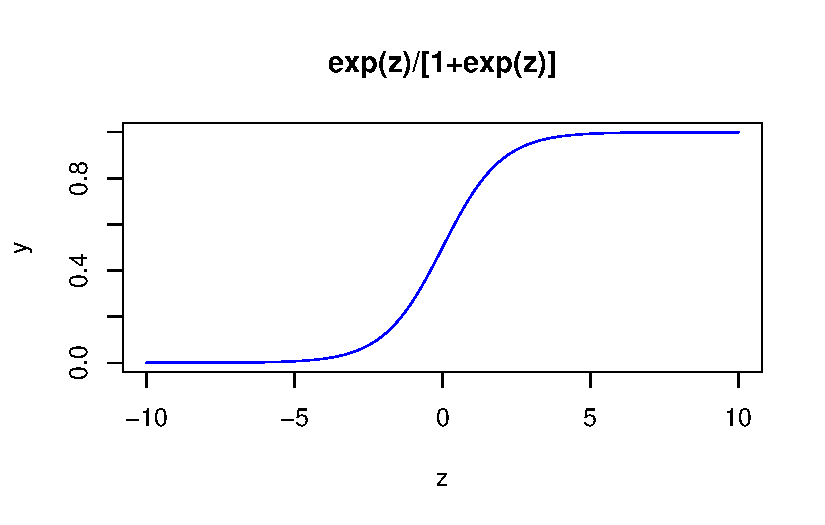
\includegraphics{cap1_files/figure-pdf/funcion-logistica-1.pdf}

Los modelos Logit y Probit pueden derivarse a partir de un
\textbf{modelo de variable latente} subyacente.

Sea \(y^*\) una variable inobservable, o \emph{latente} determianda por:

\[y^*=\beta_0+ \mathbf{x\beta}+e, y=1[y^*>0][11]\]

Aquí se introduce la notación \(1[.]\) para definir un resultado
binario. La función \(1[.]\) es la \textbf{función indicador}, que asume
valor de uno si el evento dentro de los corchetes es verdadero y cero si
es falso, Entonces tenemos:

\[y=1[y^*>0][12]\] \[y=0[y^*\leq0]\]

Se supone que \(e\) es independiente de \(\mathbf{x}\) y que \(e\) tiene
un distribución logística estándar o normal estándar. En cualquier caso,
\(e\) se distribuye simétricamente en torno a cero, lo que significa que
\(1-G(-Z)=G(z)\) para todos los números reales de \(z\).

Los economistas tienden a favorecer el supuesto de normalidad para
\(e\), lo cual es la razón por la que en Econometría el \textbf{modelo
Probit} es más popular que el \textbf{logit}. Además, varios problemas
de especificación, que se tratarán después, se analizan fácilmente
mediante Probit debido a las propiedades de la distribución normal.

Dado estos supuestos podemos calcular la probabilidad de respuesta para
\(y\):

\[P(y=1|\mathbf{x})=P(y^*>0|\mathbf{x})=P(e>-(\beta_0+\mathbf{x\beta})|\mathbf{x})=\\1-G[-(\beta_0+\mathbf{x\beta})]=G(\beta_0+\mathbf{x\beta})[13]\]
uno de los objetivos de los modelos de respuesta binaria, es explicar
los efectos de las \(x_j\) sobre la probabilidad de respuesta
\(P(y=1|\mathbf{x})\).Cuidado, la formula de la variable latente tiende
a dar la impresión de que lo que principalmente interesa son los efectos
de cada \(x_j\) sobre \(y^*\). Hay que aclarar que en los modelos Logit
y Probit la dirección de efectos de \(x_j\) sobre
\(E(y|\mathbf{x})=P(y=1|\mathbf{x})=G(\beta_0+\mathbf{x\beta})\)

Aclarando que:

\[E(y^*|\mathbf{x})=\beta_0+\mathbf{x\beta}-[14]\] Como la variable
latente pocas veces tiene una unidad de medición definida, las
magnitudes de cada \(\beta_j\) no son, útiles por sí mismas, a
diferencia de las magnitudes calculadas por el \textbf{MPL}. Entonces
para la mayoría de los propósitos, se requiere estimar el efecto de
\(x_j\) sobre la probabilidad de éxito \(P(y=1|\mathbf{x})\), esto se
complicado por la naturaleza no lineal de \(G(.)\). Esto nos lleva a
definir tres casos de efectos parciales:

\subsection{Variables aproximadamente
continuas:}\label{variables-aproximadamente-continuas}

Para hallar el efecto parcial de las variables aproximadamente continuas
sobre la probabilidad de respuesta, se recurre al cálculo. Si \(x_j\) es
una variable aproximadamente continua, su efecto parcial sobre
\(p(x)=P(y=1|\mathbf{x})\) se obtiene de la siguiente derivada parcial:

\[\frac{\partial p(\mathbf{x})}{\partial x_j}=g(\beta_0+\mathbf{x\beta})\beta_j[15]\]

Donde:

\[g(z)\equiv\frac{dG}{dz}(z) [16]\] Debido a que \(G\) es la fda de una
variable aleatoria continua, \(g\) es la función de densidad de
probabilidad.

En los casos de logit y probit, \(G(.)\) es una fda estrictamente
creciente y, por lo tanto, \(g(z)>0\forall z\). Por lo tanto, el efecto
parcial de \(x_j\) sobre \(p(\mathbf{x})\) depende de \(\mathbf{x}\) a
través de la cantidad positiva \(g(\beta_0+\mathbf{x\beta})\), lo que
significa que el efecto parcial siempre tiene el mismo signo que
\(\beta_j\)

La ecuación de la derivada parcial muestra que los efectos
\emph{relativos} del cualquiera las variables explicativas continuas no
depende de \(\mathbf{x}\), la razón de los efectos parciales de \(x_j\)
y \(x_h\) es \(\frac{\beta_j}{\beta_h}\). El caso típico de que \(g\)
sea un densidad simétrica en torno a cero, con una única moda en cero,
el mayor efecto ocurre cuando \(\beta_0+\mathbf{x\beta}=0\). Por
ejemplo:

\subsubsection{En el caso de Probit}\label{en-el-caso-de-probit}

\[g(z)=\phi(z)=\frac{e^{-z/2}}{\sqrt{2\pi}}\]
\[g(0)=\frac{e^{-0/2}}{\sqrt{2\pi}}=\frac{1}{\sqrt{2\pi}}\approx 0.40\]

\begin{Shaded}
\begin{Highlighting}[]
\DecValTok{1}\SpecialCharTok{/}\FunctionTok{sqrt}\NormalTok{(}\DecValTok{2}\SpecialCharTok{*}\NormalTok{pi)}
\end{Highlighting}
\end{Shaded}

\begin{verbatim}
[1] 0.3989423
\end{verbatim}

\subsubsection{En el caso logit}\label{en-el-caso-logit}

\[g(z)=\frac{e^z}{[1+e^z]^2}\] Evaluando cuando \(z=0\)

\[g(0)=\frac{e^0}{[1+e^0]^2}\]

\[g(0)=\frac{1}{[1+1]^2}=\frac{1}{4}=0.25\]

\subsection{Cuando la variable explicativa es
binaria}\label{cuando-la-variable-explicativa-es-binaria}

Entonces el efecto parcial de cambiar\(x_1\) de cero a uno, manteniendo
constante todas las demás variables, es así:

\[G(\beta_0+\beta_1+\beta_2x_2+...+\beta_kx_k)-G(\beta_0+\beta_2x_2+...+\beta_kx_k) [17]\]

De nuevo, esto depende de todos los valores de las otras \(x_j\). Por
ejemplo, si \(y\) es un indicador de empleo y \(x_1\) es una variable
binaria que indica la participación en un programa de capacitación
laboral, entonces es el cambio en la probabilidad de empleo debido a
este programa de capacitación; esto depende de las demás características
que afectan la posibilidad de obtener el empleo, como la educación y la
experiencia. Observe que saber el signo del \(\beta_1\) es suficiente
para determinar si el programa tuvo un efecto positivo o negativo. Pero
para hallar la \textbf{magnitud} del efecto, se tiene que estimar la
cantidad usando la anterior ecuación {[}17{]}.

\subsection{Cuando la variable explicativa es
discreta}\label{cuando-la-variable-explicativa-es-discreta}

Por ejemplo, el número de hijos. Si \(x_k\) denota esta variable, el
efecto sobre la probabilidad de que \(x_k\) cambien de \(c_k\) a
\(c_k+1\) es simplemente:

\[G[\beta_0+\beta_1x_1+\beta_2x_2+...+\beta_k(c_k+1)]-G[\beta_0+\beta_1x_1+\beta_2x_2+...+\beta_kc_k]\]

\subsection{Estimación de máxima verosimilitud de los modelos Logit y
Probit}\label{estimaciuxf3n-de-muxe1xima-verosimilitud-de-los-modelos-logit-y-probit}

Para los MPL se uso mínimos cuadrados ordinarios (MCO) o, si existe
heterocedasticidad, mínimos cuadrados ponderados (MCP). Ahora bien,
debido a naturaleza no lineal \(E(y|\mathbf{x})\), MCO y MCP no son
aplicables, por esta razón se usa la \textbf{estimación de máxima
verosimilitud (EMV)}. Para estimar los modelos de variables dependientes
limitadas, los métodos de máxima verosimilitud son indispensables. Como
la EMV está basada en la distribución de \(y\) dada \(\mathbf{x}\), la
heterocedasticidad en \(Var(y|\mathbf{x})\) automáticamente se toma en
cuenta.

Suponiendo que se tiene una muestra aleatoria \(n\). Para obtener el
estimador de máxima verosimilitud, condicional sobre las variables
explicativas, es necesario la densidad de \(y_i\) dada \(\mathbf{x_i}\).
Esto se escribe como:

\[f(y|\mathbf{x_i;\beta})=[G(\mathbf{x_i\beta})]^y[1-G(\mathbf{x_i\beta})]^{1-y},y=0,1 [17]\]

Para simplificar, se adsorbe el intercepto en el vector
\(\mathbf{x_i}\). La \textbf{función log-verosimilitud} para cada
observación \(i\) es una función de los parámetros y los datos
(\(\mathbf{x_i;y_i}\))), aplicando el logaritmo a la anterior ecuación
tenemos:

\[\mathcal{l_i(\beta)}=y_ilog[G(\mathbf{x_i\beta})]+(1-y)log[1-G(\mathbf{x_i\beta})] [18]\]
Como \(G(.)\) está estrictamente definida entre cero y uno para logit y
probit, \(\mathcal{l_i(\beta)}\) está bien definida para todos los
valores \(\beta\)

La log-verosimilitud para un tamaño de muestra \(n\) se obtiene al sumar
todas las observación de la ecuación anterior:

\[\mathcal{L_i(\beta)=\Sigma_{i=1}^n}\mathcal{l_i(\beta)}[19]\] La EMV
de \(\beta\), denotada como \(\widehat{\beta}\), maximiza esta
log-verosimilitud. Si \(G(.)\) es la fda logit estándar, entonces
\(\widehat{\beta}\) será el estimador Logit; si \(G(.)\) es la fda
normal estándar, entonces \(\widehat{\beta}\) será el estimador Probit.

\subsection{Ejemplos de aplicación}\label{ejemplos-de-aplicaciuxf3n}

Continuaremos con los ejemplos usados en el MPL, como son: la
Participación en la fuerza laboral de las mujeres casadas, un modelo de
probabilidad para arrestos y, sumaremos el ejemplo de la denegación de
una hipoteca (Stock and Watson 2012)

\subsubsection{Logit para los datos
HMDA}\label{logit-para-los-datos-hmda}

\begin{Shaded}
\begin{Highlighting}[]
\FunctionTok{library}\NormalTok{(AER)}
\FunctionTok{data}\NormalTok{(HMDA)}

\NormalTok{HMDA }\SpecialCharTok{|\textgreater{}}
  \FunctionTok{str}\NormalTok{()}
\end{Highlighting}
\end{Shaded}

\begin{verbatim}
'data.frame':   2380 obs. of  14 variables:
 $ deny     : Factor w/ 2 levels "no","yes": 1 1 1 1 1 1 1 1 2 1 ...
 $ pirat    : num  0.221 0.265 0.372 0.32 0.36 ...
 $ hirat    : num  0.221 0.265 0.248 0.25 0.35 ...
 $ lvrat    : num  0.8 0.922 0.92 0.86 0.6 ...
 $ chist    : Factor w/ 6 levels "1","2","3","4",..: 5 2 1 1 1 1 1 2 2 2 ...
 $ mhist    : Factor w/ 4 levels "1","2","3","4": 2 2 2 2 1 1 2 2 2 1 ...
 $ phist    : Factor w/ 2 levels "no","yes": 1 1 1 1 1 1 1 1 1 1 ...
 $ unemp    : num  3.9 3.2 3.2 4.3 3.2 ...
 $ selfemp  : Factor w/ 2 levels "no","yes": 1 1 1 1 1 1 1 1 1 1 ...
 $ insurance: Factor w/ 2 levels "no","yes": 1 1 1 1 1 1 1 1 2 1 ...
 $ condomin : Factor w/ 2 levels "no","yes": 1 1 1 1 1 1 2 1 1 1 ...
 $ afam     : Factor w/ 2 levels "no","yes": 1 1 1 1 1 1 1 1 1 1 ...
 $ single   : Factor w/ 2 levels "no","yes": 1 2 1 1 1 1 2 1 1 2 ...
 $ hschool  : Factor w/ 2 levels "no","yes": 2 2 2 2 2 2 2 2 2 2 ...
\end{verbatim}

\subsubsection{La participación den la fuerza laboral de las mujeres
casadas}\label{la-participaciuxf3n-den-la-fuerza-laboral-de-las-mujeres-casadas}

\paragraph{Modelo Probit estimado con fda normal
estándar}\label{modelo-probit-estimado-con-fda-normal-estuxe1ndar}

Para estimar modelos de variable dependiente limitada se usa el comando
\emph{glm()}

\begin{Shaded}
\begin{Highlighting}[]
\FunctionTok{data}\NormalTok{(}\StringTok{"mroz"}\NormalTok{, }\AttributeTok{package =} \StringTok{"wooldridge"}\NormalTok{)}

\NormalTok{MPL.mroz }\OtherTok{\textless{}{-}}\FunctionTok{lm}\NormalTok{(inlf}\SpecialCharTok{\textasciitilde{}}
\NormalTok{                 nwifeinc}\SpecialCharTok{+}
\NormalTok{                 educ}\SpecialCharTok{+}
\NormalTok{                 exper}\SpecialCharTok{+}
\NormalTok{                 expersq}\SpecialCharTok{+}
\NormalTok{                 age}\SpecialCharTok{+}
\NormalTok{                 kidslt6}\SpecialCharTok{+}
\NormalTok{                 kidsge6,}
               \AttributeTok{data =}\NormalTok{ mroz) }


\NormalTok{mroz.probit }\OtherTok{\textless{}{-}} \FunctionTok{glm}\NormalTok{(inlf}\SpecialCharTok{\textasciitilde{}}
\NormalTok{                 nwifeinc}\SpecialCharTok{+}
\NormalTok{                 educ}\SpecialCharTok{+}
\NormalTok{                 exper}\SpecialCharTok{+}
\NormalTok{                 expersq}\SpecialCharTok{+}
\NormalTok{                 age}\SpecialCharTok{+}
\NormalTok{                 kidslt6}\SpecialCharTok{+}
\NormalTok{                 kidsge6,}
               \AttributeTok{data =}\NormalTok{ mroz,}
               \AttributeTok{family =} \FunctionTok{binomial}\NormalTok{(}\AttributeTok{link =} \StringTok{"probit"}\NormalTok{))}

\FunctionTok{library}\NormalTok{(stargazer)}
\FunctionTok{stargazer}\NormalTok{(MPL.mroz, mroz.probit, }\AttributeTok{type =} \StringTok{"text"}\NormalTok{)}
\end{Highlighting}
\end{Shaded}

\begin{verbatim}

=====================================================
                           Dependent variable:       
                    ---------------------------------
                                  inlf               
                              OLS            probit  
                              (1)              (2)   
-----------------------------------------------------
nwifeinc                   -0.003**         -0.012** 
                            (0.001)          (0.005) 
                                                     
educ                       0.038***         0.131*** 
                            (0.007)          (0.025) 
                                                     
exper                      0.039***         0.123*** 
                            (0.006)          (0.019) 
                                                     
expersq                    -0.001***        -0.002***
                           (0.0002)          (0.001) 
                                                     
age                        -0.016***        -0.053***
                            (0.002)          (0.008) 
                                                     
kidslt6                    -0.262***        -0.868***
                            (0.034)          (0.118) 
                                                     
kidsge6                      0.013            0.036  
                            (0.013)          (0.044) 
                                                     
Constant                   0.586***           0.270  
                            (0.154)          (0.508) 
                                                     
-----------------------------------------------------
Observations                  753              753   
R2                           0.264                   
Adjusted R2                  0.257                   
Log Likelihood                              -401.302 
Akaike Inf. Crit.                            818.604 
Residual Std. Error    0.427 (df = 745)              
F Statistic         38.218*** (df = 7; 745)          
=====================================================
Note:                     *p<0.1; **p<0.05; ***p<0.01
\end{verbatim}

\subparagraph{¿Cómo funciona la mecánica del modelo
Probit?}\label{cuxf3mo-funciona-la-mecuxe1nica-del-modelo-probit}

\begin{Shaded}
\begin{Highlighting}[]
\NormalTok{mroz.probit.simple }\OtherTok{\textless{}{-}}\FunctionTok{glm}\NormalTok{(inlf}\SpecialCharTok{\textasciitilde{}}
\NormalTok{                           kidslt6,}
                         \AttributeTok{data =}\NormalTok{ mroz,}
                         \AttributeTok{family =} \FunctionTok{binomial}\NormalTok{(}\AttributeTok{link =} \StringTok{"probit"}\NormalTok{))}

\NormalTok{mroz.probit.simple1 }\OtherTok{\textless{}{-}}\FunctionTok{glm}\NormalTok{(inlf}\SpecialCharTok{\textasciitilde{}}
\NormalTok{                           nwifeinc,}
                         \AttributeTok{data =}\NormalTok{ mroz,}
                         \AttributeTok{family =} \FunctionTok{binomial}\NormalTok{(}\AttributeTok{link =} \StringTok{"probit"}\NormalTok{))}

\NormalTok{stargazer}\SpecialCharTok{::}\FunctionTok{stargazer}\NormalTok{(mroz.probit.simple1, }\AttributeTok{type =} \StringTok{"text"}\NormalTok{)}
\end{Highlighting}
\end{Shaded}

\begin{verbatim}

=============================================
                      Dependent variable:    
                  ---------------------------
                             inlf            
---------------------------------------------
nwifeinc                   -0.013***         
                            (0.004)          
                                             
Constant                   0.432***          
                            (0.094)          
                                             
---------------------------------------------
Observations                  753            
Log Likelihood             -509.662          
Akaike Inf. Crit.          1,023.324         
=============================================
Note:             *p<0.1; **p<0.05; ***p<0.01
\end{verbatim}

\begin{Shaded}
\begin{Highlighting}[]
\FunctionTok{mean}\NormalTok{(mroz}\SpecialCharTok{$}\NormalTok{kidslt6)}
\end{Highlighting}
\end{Shaded}

\begin{verbatim}
[1] 0.2377158
\end{verbatim}

\begin{Shaded}
\begin{Highlighting}[]
\CommentTok{\# EFectos en cambios puntuales}

\NormalTok{prediccion}\OtherTok{\textless{}{-}}\FunctionTok{predict}\NormalTok{(mroz.probit.simple,}
                    \AttributeTok{newdata=}\FunctionTok{data.frame}\NormalTok{(}\StringTok{"kidslt6"}\OtherTok{=}\FunctionTok{c}\NormalTok{(}\DecValTok{1}\NormalTok{,}\DecValTok{2}\NormalTok{)),}
                    \AttributeTok{type =} \StringTok{"response"}\NormalTok{)}

\FunctionTok{diff}\NormalTok{(prediccion)}\SpecialCharTok{*}\DecValTok{100}
\end{Highlighting}
\end{Shaded}

\begin{verbatim}
       2 
-18.7173 
\end{verbatim}

\subsubsection{Presentación del modelo
estimado}\label{presentaciuxf3n-del-modelo-estimado}

\textbf{Modelo probit simple}

\[
\widehat{P(infl=1|kidslt6)}=\Phi \left(0.299-0.539kidslt6\right)
\]

\begin{Shaded}
\begin{Highlighting}[]
\FunctionTok{pnorm}\NormalTok{(}\FunctionTok{coef}\NormalTok{(mroz.probit.simple)[}\DecValTok{1}\NormalTok{]}\SpecialCharTok{+}\FunctionTok{coef}\NormalTok{(mroz.probit.simple)[}\DecValTok{2}\NormalTok{]}\SpecialCharTok{*}\DecValTok{2}\NormalTok{)}\SpecialCharTok{{-}}\FunctionTok{pnorm}\NormalTok{(}\FunctionTok{coef}\NormalTok{(mroz.probit.simple)[}\DecValTok{1}\NormalTok{]}\SpecialCharTok{+}\FunctionTok{coef}\NormalTok{(mroz.probit.simple)[}\DecValTok{2}\NormalTok{]}\SpecialCharTok{*}\DecValTok{1}\NormalTok{)}
\end{Highlighting}
\end{Shaded}

\begin{verbatim}
(Intercept) 
  -0.187173 
\end{verbatim}

\textbf{Ecuación estimada de probit}

\begin{Shaded}
\begin{Highlighting}[]
\FunctionTok{coef}\NormalTok{(mroz.probit)}
\end{Highlighting}
\end{Shaded}

\begin{verbatim}
 (Intercept)     nwifeinc         educ        exper      expersq          age 
 0.270073573 -0.012023637  0.130903969  0.123347168 -0.001887067 -0.052852442 
     kidslt6      kidsge6 
-0.868324680  0.036005611 
\end{verbatim}

\[
\begin{aligned}
P(inlf&=1|nwifeinc,...,kidsge6)=\\
&\Phi(0.27-0.012nwifeinc+0.131educ+0.12exper\\
&-0.0019exper^2-0.053age-0.87kidslt6+0.036kidsg6)
\end{aligned}
\]

¿Cuál es la probabilidad de salir de que María salga a trabajar, dado
que tiene su esposo un ingreso mensual 300USD, tiene 4 años de
educación, nunca ha trabajo, tiene 29 años y un niño de 3 años?

\begin{Shaded}
\begin{Highlighting}[]
\FunctionTok{coef}\NormalTok{(mroz.probit)}
\end{Highlighting}
\end{Shaded}

\begin{verbatim}
 (Intercept)     nwifeinc         educ        exper      expersq          age 
 0.270073573 -0.012023637  0.130903969  0.123347168 -0.001887067 -0.052852442 
     kidslt6      kidsge6 
-0.868324680  0.036005611 
\end{verbatim}

\begin{Shaded}
\begin{Highlighting}[]
\CommentTok{\# Pregunta inicial}
\NormalTok{prediccion}\OtherTok{\textless{}{-}}\FunctionTok{predict}\NormalTok{(mroz.probit,}
                    \AttributeTok{newdata=}\FunctionTok{data.frame}\NormalTok{(}\StringTok{"nwifeinc"}\OtherTok{=}\NormalTok{(}\DecValTok{300}\SpecialCharTok{*}\DecValTok{12}\NormalTok{)}\SpecialCharTok{/}\DecValTok{1000}\NormalTok{,}
                                       \StringTok{"educ"}\OtherTok{=}\DecValTok{4}\NormalTok{,}
                                       \StringTok{"exper"}\OtherTok{=}\DecValTok{0}\NormalTok{,}
                                       \StringTok{"expersq"}\OtherTok{=}\DecValTok{0}\NormalTok{,}
                                       \StringTok{"age"}\OtherTok{=}\DecValTok{29}\NormalTok{,}
                                       \StringTok{"kidslt6"}\OtherTok{=}\DecValTok{1}\NormalTok{,}
                                       \StringTok{"kidsge6"}\OtherTok{=}\DecValTok{0}\NormalTok{),}
                    \AttributeTok{type =} \StringTok{"response"}\NormalTok{)}

\FunctionTok{predict}\NormalTok{(mroz.probit,}
                    \AttributeTok{newdata=}\FunctionTok{data.frame}\NormalTok{(}\StringTok{"nwifeinc"}\OtherTok{=}\NormalTok{(}\DecValTok{300}\SpecialCharTok{*}\DecValTok{12}\NormalTok{)}\SpecialCharTok{/}\DecValTok{1000}\NormalTok{,}
                                       \StringTok{"educ"}\OtherTok{=}\DecValTok{4}\NormalTok{,}
                                       \StringTok{"exper"}\OtherTok{=}\DecValTok{0}\NormalTok{,}
                                       \StringTok{"expersq"}\OtherTok{=}\DecValTok{0}\NormalTok{,}
                                       \StringTok{"age"}\OtherTok{=}\DecValTok{29}\SpecialCharTok{+}\DecValTok{3}\NormalTok{,}
                                       \StringTok{"kidslt6"}\OtherTok{=}\DecValTok{1}\NormalTok{,}
                                       \StringTok{"kidsge6"}\OtherTok{=}\DecValTok{1}\NormalTok{),}
                    \AttributeTok{type =} \StringTok{"response"}\NormalTok{)}
\end{Highlighting}
\end{Shaded}

\begin{verbatim}
         1 
0.03809838 
\end{verbatim}

\begin{Shaded}
\begin{Highlighting}[]
\CommentTok{\#Diferencia}
\NormalTok{cambio }\OtherTok{\textless{}{-}} \FunctionTok{predict}\NormalTok{(mroz.probit,}
                    \AttributeTok{newdata=}\FunctionTok{data.frame}\NormalTok{(}\StringTok{"nwifeinc"}\OtherTok{=}\NormalTok{(}\DecValTok{300}\SpecialCharTok{*}\DecValTok{12}\NormalTok{)}\SpecialCharTok{/}\DecValTok{1000}\NormalTok{,}
                                       \StringTok{"educ"}\OtherTok{=}\DecValTok{4}\NormalTok{,}
                                       \StringTok{"exper"}\OtherTok{=}\DecValTok{0}\NormalTok{,}
                                       \StringTok{"expersq"}\OtherTok{=}\DecValTok{0}\NormalTok{,}
                                       \StringTok{"age"}\OtherTok{=}\FunctionTok{c}\NormalTok{(}\DecValTok{29}\NormalTok{,}\DecValTok{29}\SpecialCharTok{+}\DecValTok{3}\NormalTok{),}
                                       \StringTok{"kidslt6"}\OtherTok{=}\DecValTok{1}\NormalTok{,}
                                       \StringTok{"kidsge6"}\OtherTok{=}\FunctionTok{c}\NormalTok{(}\DecValTok{0}\NormalTok{,}\DecValTok{1}\NormalTok{)),}
                    \AttributeTok{type =} \StringTok{"response"}\NormalTok{)}

\FunctionTok{diff}\NormalTok{(cambio)}\SpecialCharTok{*}\DecValTok{100}
\end{Highlighting}
\end{Shaded}

\begin{verbatim}
        2 
-1.130756 
\end{verbatim}

\begin{Shaded}
\begin{Highlighting}[]
\CommentTok{\# En el MPL}

\NormalTok{cambio.MPL }\OtherTok{\textless{}{-}} \FunctionTok{predict}\NormalTok{(MPL.mroz,}
                    \AttributeTok{newdata=}\FunctionTok{data.frame}\NormalTok{(}\StringTok{"nwifeinc"}\OtherTok{=}\NormalTok{(}\DecValTok{300}\SpecialCharTok{*}\DecValTok{12}\NormalTok{)}\SpecialCharTok{/}\DecValTok{1000}\NormalTok{,}
                                       \StringTok{"educ"}\OtherTok{=}\DecValTok{4}\NormalTok{,}
                                       \StringTok{"exper"}\OtherTok{=}\DecValTok{0}\NormalTok{,}
                                       \StringTok{"expersq"}\OtherTok{=}\DecValTok{0}\NormalTok{,}
                                       \StringTok{"age"}\OtherTok{=}\FunctionTok{c}\NormalTok{(}\DecValTok{29}\NormalTok{,}\DecValTok{29}\SpecialCharTok{+}\DecValTok{3}\NormalTok{),}
                                       \StringTok{"kidslt6"}\OtherTok{=}\DecValTok{1}\NormalTok{,}
                                       \StringTok{"kidsge6"}\OtherTok{=}\FunctionTok{c}\NormalTok{(}\DecValTok{0}\NormalTok{,}\DecValTok{1}\NormalTok{)),}
                    \AttributeTok{type =} \StringTok{"response"}\NormalTok{)}

\FunctionTok{diff}\NormalTok{(cambio.MPL)}\SpecialCharTok{*}\DecValTok{100}
\end{Highlighting}
\end{Shaded}

\begin{verbatim}
        2 
-3.526018 
\end{verbatim}

\subsubsection{Modelo Logit estimado con FDA logística
estándar}\label{modelo-logit-estimado-con-fda-loguxedstica-estuxe1ndar}

\begin{Shaded}
\begin{Highlighting}[]
\NormalTok{mroz.logit }\OtherTok{\textless{}{-}} \FunctionTok{glm}\NormalTok{(inlf}\SpecialCharTok{\textasciitilde{}}
\NormalTok{                 nwifeinc}\SpecialCharTok{+}
\NormalTok{                 educ}\SpecialCharTok{+}
\NormalTok{                 exper}\SpecialCharTok{+}
\NormalTok{                 expersq}\SpecialCharTok{+}
\NormalTok{                 age}\SpecialCharTok{+}
\NormalTok{                 kidslt6}\SpecialCharTok{+}
\NormalTok{                 kidsge6,}
               \AttributeTok{data =}\NormalTok{ mroz,}
               \AttributeTok{family =} \FunctionTok{binomial}\NormalTok{(}\AttributeTok{link =} \StringTok{"logit"}\NormalTok{))}

\FunctionTok{stargazer}\NormalTok{(mroz.logit, }\AttributeTok{type =} \StringTok{"text"}\NormalTok{)}
\end{Highlighting}
\end{Shaded}

\begin{verbatim}

=============================================
                      Dependent variable:    
                  ---------------------------
                             inlf            
---------------------------------------------
nwifeinc                   -0.021**          
                            (0.008)          
                                             
educ                       0.221***          
                            (0.043)          
                                             
exper                      0.206***          
                            (0.032)          
                                             
expersq                    -0.003***         
                            (0.001)          
                                             
age                        -0.088***         
                            (0.015)          
                                             
kidslt6                    -1.443***         
                            (0.204)          
                                             
kidsge6                      0.060           
                            (0.075)          
                                             
Constant                     0.425           
                            (0.860)          
                                             
---------------------------------------------
Observations                  753            
Log Likelihood             -401.765          
Akaike Inf. Crit.           819.530          
=============================================
Note:             *p<0.1; **p<0.05; ***p<0.01
\end{verbatim}

\subparagraph{¿Cómo funciona la mecánica del modelo
Logit?}\label{cuxf3mo-funciona-la-mecuxe1nica-del-modelo-logit}

\begin{Shaded}
\begin{Highlighting}[]
\NormalTok{mroz.logit.simple }\OtherTok{\textless{}{-}}\FunctionTok{glm}\NormalTok{(inlf}\SpecialCharTok{\textasciitilde{}}
\NormalTok{                           kidslt6,}
                         \AttributeTok{data =}\NormalTok{ mroz,}
                         \AttributeTok{family =} \FunctionTok{binomial}\NormalTok{(}\AttributeTok{link =} \StringTok{"logit"}\NormalTok{))}

\FunctionTok{stargazer}\NormalTok{(mroz.probit.simple, }\AttributeTok{type =} \StringTok{"text"}\NormalTok{)}
\end{Highlighting}
\end{Shaded}

\begin{verbatim}

=============================================
                      Dependent variable:    
                  ---------------------------
                             inlf            
---------------------------------------------
kidslt6                    -0.539***         
                            (0.094)          
                                             
Constant                   0.299***          
                            (0.051)          
                                             
---------------------------------------------
Observations                  753            
Log Likelihood             -497.367          
Akaike Inf. Crit.           998.734          
=============================================
Note:             *p<0.1; **p<0.05; ***p<0.01
\end{verbatim}

\begin{Shaded}
\begin{Highlighting}[]
\CommentTok{\# EFectos en cambios puntuales}

\NormalTok{prediccion}\OtherTok{\textless{}{-}}\FunctionTok{predict}\NormalTok{(mroz.logit.simple,}
                    \AttributeTok{newdata=}\FunctionTok{data.frame}\NormalTok{(}\StringTok{"kidslt6"}\OtherTok{=}\FunctionTok{c}\NormalTok{(}\DecValTok{1}\NormalTok{,}\DecValTok{2}\NormalTok{)),}
                    \AttributeTok{type =} \StringTok{"response"}\NormalTok{)}
\FunctionTok{diff}\NormalTok{(prediccion)}\SpecialCharTok{*}\DecValTok{100}
\end{Highlighting}
\end{Shaded}

\begin{verbatim}
        2 
-18.29326 
\end{verbatim}

\begin{Shaded}
\begin{Highlighting}[]
\NormalTok{lambda }\OtherTok{\textless{}{-}} \ControlFlowTok{function}\NormalTok{(z) }\DecValTok{1}\SpecialCharTok{/}\NormalTok{(}\DecValTok{1}\SpecialCharTok{+}\FunctionTok{exp}\NormalTok{(}\SpecialCharTok{{-}}\NormalTok{z))}

\FunctionTok{lambda}\NormalTok{(}\FunctionTok{coef}\NormalTok{(mroz.logit.simple)[}\DecValTok{1}\NormalTok{]}\SpecialCharTok{+}\FunctionTok{coef}\NormalTok{(mroz.logit.simple)[}\DecValTok{2}\NormalTok{]}\SpecialCharTok{*}\DecValTok{2}\NormalTok{)}\SpecialCharTok{*}\DecValTok{100}\SpecialCharTok{{-}}\FunctionTok{lambda}\NormalTok{(}\FunctionTok{coef}\NormalTok{(mroz.logit.simple)[}\DecValTok{1}\NormalTok{]}\SpecialCharTok{+}\FunctionTok{coef}\NormalTok{(mroz.logit.simple)[}\DecValTok{2}\NormalTok{]}\SpecialCharTok{*}\DecValTok{1}\NormalTok{)}\SpecialCharTok{*}\DecValTok{100}
\end{Highlighting}
\end{Shaded}

\begin{verbatim}
(Intercept) 
  -18.29326 
\end{verbatim}

\begin{Shaded}
\begin{Highlighting}[]
\CommentTok{\# Verificando que las probabilidades ajustadas se encuentren entre 0 y 1}

\FunctionTok{summary}\NormalTok{(mroz.probit}\SpecialCharTok{$}\NormalTok{fitted.values)}
\end{Highlighting}
\end{Shaded}

\begin{verbatim}
    Min.  1st Qu.   Median     Mean  3rd Qu.     Max. 
0.002475 0.370959 0.609546 0.570109 0.794345 0.979904 
\end{verbatim}

\begin{Shaded}
\begin{Highlighting}[]
\FunctionTok{summary}\NormalTok{(mroz.logit}\SpecialCharTok{$}\NormalTok{fitted.values)}
\end{Highlighting}
\end{Shaded}

\begin{verbatim}
    Min.  1st Qu.   Median     Mean  3rd Qu.     Max. 
0.008672 0.366410 0.610925 0.568393 0.796721 0.968541 
\end{verbatim}

\textbf{Presentación del modelo estimado}

\[P(inlf=1|nwifeinc,...,kidsge6)=\Lambda(0.425-0.021nwifeinc+...+0.060kidsge6)\]

\subsubsection{Comparación de los modelos MPL, Logit y
Probit}\label{comparaciuxf3n-de-los-modelos-mpl-logit-y-probit}

Para esta comparación se va usar los errores heterocedástico robustos.

\begin{Shaded}
\begin{Highlighting}[]
\FunctionTok{library}\NormalTok{(sandwich)}

\NormalTok{eher}\OtherTok{\textless{}{-}}\FunctionTok{list}\NormalTok{(}\FunctionTok{sqrt}\NormalTok{(}\FunctionTok{diag}\NormalTok{(}\FunctionTok{vcovHC}\NormalTok{(MPL.mroz, }\AttributeTok{type =} \StringTok{"HC1"}\NormalTok{))),}
           \FunctionTok{sqrt}\NormalTok{(}\FunctionTok{diag}\NormalTok{(}\FunctionTok{vcovHC}\NormalTok{(mroz.logit, }\AttributeTok{type =} \StringTok{"HC1"}\NormalTok{))),}
           \FunctionTok{sqrt}\NormalTok{(}\FunctionTok{diag}\NormalTok{(}\FunctionTok{vcovHC}\NormalTok{(mroz.probit, }\AttributeTok{type =} \StringTok{"HC1"}\NormalTok{))))}

\FunctionTok{stargazer}\NormalTok{(MPL.mroz, mroz.logit, mroz.probit,}
          \AttributeTok{se =}\NormalTok{ eher,}
          \AttributeTok{digits =} \DecValTok{3}\NormalTok{,}
          \AttributeTok{type =} \StringTok{"text"}\NormalTok{,}
          \AttributeTok{title =} \StringTok{"Tabla 2: Estimaciones MPL, logit y probit de la participación en la fuerza laboral"}\NormalTok{,}
          \AttributeTok{df=}\NormalTok{F,}
          \AttributeTok{header =}\NormalTok{ F)}
\end{Highlighting}
\end{Shaded}

\begin{verbatim}

Tabla 2: Estimaciones MPL, logit y probit de la participación en la fuerza laboral
=================================================
                         Dependent variable:     
                    -----------------------------
                                inlf             
                       OLS    logistic   probit  
                       (1)       (2)       (3)   
-------------------------------------------------
nwifeinc            -0.003**  -0.021**  -0.012** 
                     (0.002)   (0.009)   (0.006) 
                                                 
educ                0.038***  0.221***  0.131*** 
                     (0.007)   (0.045)   (0.026) 
                                                 
exper               0.039***  0.206***  0.123*** 
                     (0.006)   (0.032)   (0.019) 
                                                 
expersq             -0.001*** -0.003*** -0.002***
                    (0.0002)   (0.001)   (0.001) 
                                                 
age                 -0.016*** -0.088*** -0.053***
                     (0.002)   (0.015)   (0.008) 
                                                 
kidslt6             -0.262*** -1.443*** -0.868***
                     (0.032)   (0.204)   (0.117) 
                                                 
kidsge6               0.013     0.060     0.036  
                     (0.014)   (0.080)   (0.047) 
                                                 
Constant            0.586***    0.425     0.270  
                     (0.152)   (0.864)   (0.507) 
                                                 
-------------------------------------------------
Observations           753       753       753   
R2                    0.264                      
Adjusted R2           0.257                      
Log Likelihood                -401.765  -401.302 
Akaike Inf. Crit.              819.530   818.604 
Residual Std. Error   0.427                      
F Statistic         38.218***                    
=================================================
Note:                 *p<0.1; **p<0.05; ***p<0.01
\end{verbatim}

Como podemos ver en la tabla 2 los signos y la significancia es la misma
para todas las variables en los tres modelos. Por ejemplo, la variable
\emph{educ} y \emph{exper} son estadísticamente significativas en los
tres modelos y ambas tienen un signo positivo respecto a la probabilidad
de la participación en la fuerza laboral de las mujeres. En un primer
momento no es posible comparar las estimaciones logit y probit con las
del MPL. Para hacerlas comparables se debe usar el \textbf{efecto
parcial promedio (EPP)}. Wooldridge (2010, 585) siguiere factores
escalares que se deben pre-multiplicar por los coeficientes de logit y
probit para hacerlos comparables con el MPL. Para Probit es 0.301 y para
logit es 0.179.

\textbf{Usando factores escalares logit y probit para comparar con
coeficientes MPL}

El ejemplo de la variable \emph{educ}. Si multiplico el coeficiente de
\emph{educ} en logit por su factor se obtiene:
\(0.179(0.221)\approx0.040\) y coeficiente probit \emph{educ} es de
alrededor de \(0.301(0.131)\approx0.039\).Como se puede observar, ambos
coeficientes son muy cercanos a la estimación de MPL que es de
\(0.038\). También la variable discreta \emph{kidslt6}, los coeficientes
escalados logit y probit son similares al coeficiente del MPL de
\(-0.262\). Estos son \(0.179(-1.443)\approx-0.258\) (logit) y,
\(0.301(-0.868)\approx-0.261\) (probit)

La mayor diferencia entre el modelo MPL y los modelos logit y probit es
que el MPL supone efectos \emph{constantes} para \emph{educ},
\emph{exper}, \emph{kidslt6}, etc., mientras que los modelos logit y
probit implican magnitudes decrecientes de los efectos parciales

\subsubsection{Curva decreciente}\label{curva-decreciente}

En esta sección vamos a observar como los modelos no lineales logit y
probit muestran que no es lo mismo tener niño pequeño, dos o tres, etc,
para reducir la probabilidad de salir a trabajar

\begin{Shaded}
\begin{Highlighting}[]
\NormalTok{mpl.simple }\OtherTok{\textless{}{-}} \FunctionTok{lm}\NormalTok{(inlf}\SpecialCharTok{\textasciitilde{}}
\NormalTok{                   kidslt6,}
\NormalTok{                 mroz)}
\FunctionTok{plot}\NormalTok{(}\AttributeTok{x =}\NormalTok{ mroz}\SpecialCharTok{$}\NormalTok{kidslt6,}
     \AttributeTok{y=}\NormalTok{ mroz}\SpecialCharTok{$}\NormalTok{inlf,}
     \AttributeTok{main =} \StringTok{"Modelo probit para los determinates del trabajo femenino"}\NormalTok{,}
     \AttributeTok{xlab =} \StringTok{"Niños menore a seis años"}\NormalTok{,}
     \AttributeTok{ylab =} \StringTok{"Infl, si una mujer casada sale a trabajar por un salario"}\NormalTok{,}
     \AttributeTok{pch=}\DecValTok{20}\NormalTok{,}
     \AttributeTok{ylim =} \FunctionTok{c}\NormalTok{(}\SpecialCharTok{{-}}\FloatTok{0.4}\NormalTok{, }\FloatTok{1.4}\NormalTok{),}
     \AttributeTok{xlim =} \FunctionTok{c}\NormalTok{(}\SpecialCharTok{{-}}\FloatTok{0.2}\NormalTok{,}\DecValTok{8}\NormalTok{))}
\FunctionTok{grid}\NormalTok{()}
\CommentTok{\# Añadir las lineas horizontales y el texto}
\FunctionTok{abline}\NormalTok{(}\AttributeTok{h=}\DecValTok{1}\NormalTok{, }\AttributeTok{lty=}\DecValTok{2}\NormalTok{, }\AttributeTok{col=}\StringTok{"darkred"}\NormalTok{)}
\FunctionTok{abline}\NormalTok{(}\AttributeTok{h=}\DecValTok{0}\NormalTok{, }\AttributeTok{lty=}\DecValTok{2}\NormalTok{, }\AttributeTok{col=}\StringTok{"darkred"}\NormalTok{)}
\FunctionTok{text}\NormalTok{(}\FloatTok{2.5}\NormalTok{, }\FloatTok{0.9}\NormalTok{, }\AttributeTok{cex =} \FloatTok{0.8}\NormalTok{, }\StringTok{"Sale a trabajar"}\NormalTok{)}
\FunctionTok{text}\NormalTok{(}\FloatTok{2.5}\NormalTok{, }\SpecialCharTok{{-}}\FloatTok{0.1}\NormalTok{, }\AttributeTok{cex =} \FloatTok{0.8}\NormalTok{, }\StringTok{"No sale a trabajar"}\NormalTok{)}

\CommentTok{\# añadiendo la linea de regresión probit}
\NormalTok{x }\OtherTok{\textless{}{-}} \FunctionTok{seq}\NormalTok{(}\DecValTok{0}\NormalTok{,}\DecValTok{7}\NormalTok{,}\DecValTok{1}\NormalTok{)}
\NormalTok{y }\OtherTok{\textless{}{-}} \FunctionTok{predict}\NormalTok{(mroz.probit.simple, }
             \FunctionTok{list}\NormalTok{(}\AttributeTok{kidslt6=}\NormalTok{x), }
             \AttributeTok{type =} \StringTok{"response"}\NormalTok{)}
\FunctionTok{lines}\NormalTok{(x,y,}\AttributeTok{lwd=}\FloatTok{1.5}\NormalTok{, }\AttributeTok{col=}\StringTok{"steelblue"}\NormalTok{)}

\CommentTok{\# añadiendo la linea de regresión logit}

\NormalTok{t }\OtherTok{\textless{}{-}} \FunctionTok{predict}\NormalTok{(mroz.logit.simple, }
             \FunctionTok{list}\NormalTok{(}\AttributeTok{kidslt6=}\NormalTok{x), }
             \AttributeTok{type =} \StringTok{"response"}\NormalTok{)}
\FunctionTok{lines}\NormalTok{(x,t,}\AttributeTok{lwd=}\FloatTok{1.5}\NormalTok{, }\AttributeTok{col=}\StringTok{"pink"}\NormalTok{)}

\CommentTok{\# añadiendo la linea de regresión MPL}

\NormalTok{m }\OtherTok{\textless{}{-}} \FunctionTok{predict}\NormalTok{(mpl.simple, }
             \FunctionTok{list}\NormalTok{(}\AttributeTok{kidslt6=}\NormalTok{x), }
             \AttributeTok{type =} \StringTok{"response"}\NormalTok{)}
\FunctionTok{lines}\NormalTok{(x,m,}\AttributeTok{lwd=}\FloatTok{1.5}\NormalTok{, }\AttributeTok{col=}\StringTok{"green"}\NormalTok{)}
\end{Highlighting}
\end{Shaded}

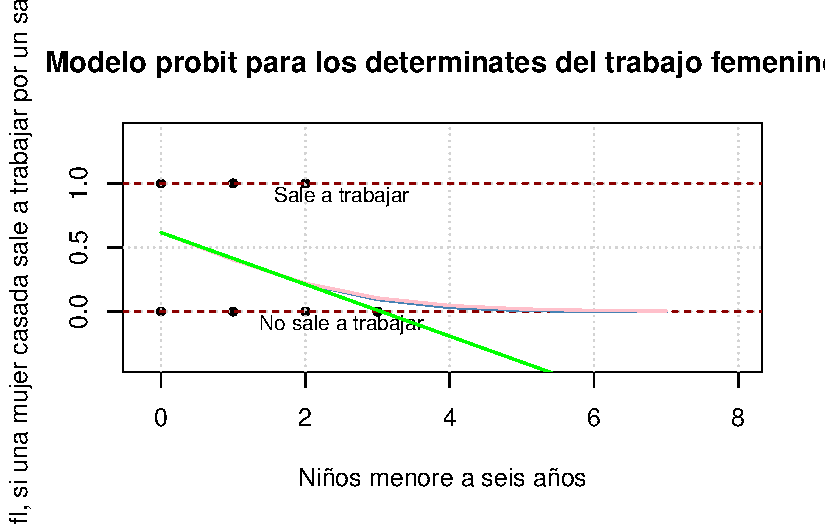
\includegraphics{cap1_files/figure-pdf/Curva decreciente-1.pdf}

\subsection{Interpretaciones de las estimaciones Logit y
Probit}\label{interpretaciones-de-las-estimaciones-logit-y-probit}

Las estimaciones de coeficientes, sus errores estándar y el valor de la
función de log-verosimilitud se pueden obtener mediante todos los
paquetes de software (R) que realicen logit y probit, y se deben
reportar en cualquier aplicación. Los coeficientes dan los signos de los
efectos parciales de cada \(x_j\) sobre la probabilidad de respuesta y
la significancia estadística de \(x_j\) está determinada por si se puede
rechazar \(H_0:\beta_j=0\) a un nivel de significancia (\(\alpha\)).

Como vimos anteriormente para el MPL se puede calcular el
\textbf{porcentaje predicho correctamente}

Existen varias medidas de bondad de ajuste como \textbf{pseudo
R-cuadradas}. MacFadden (1974) sugiere la medida
\(1-\frac{\mathscr{L}_{nr}}{\mathscr{L}_{o}}\), donde
\(\mathscr{L}_{nr}\) es la función de log-verosimilitud para el modelo
estimado y,\(\mathscr{L}_{o}\) es la función de probabilidad de log en
el modelo con sólo un intercepto. ¿Por qué esta medida es lógica?
Recordar que las log-verosimilitud son negativas y, por tanto
\(\frac{\mathscr{L}_{nr}}{\mathscr{L}_{o}}=\frac{|\mathscr{L}_{nr}|}{|\mathscr{L}_{o}|}\).
Además. \(|\mathscr{L}_{nr}|\leq|\mathscr{L}_{o}|\). Si las covarianzas
no tiene poder explicativo, entonces
\(\frac{\mathscr{L}_{nr}}{\mathscr{L}_{o}}=1\), la \textbf{pseudo
R-cuadrada} será igual a cero, como la R-cuadrada usual es cero en una
regresión lineal cuando las covariadas no tienen poder explicativo.

Por lo general, \(|\mathscr{L}_{nr}|<|\mathscr{L}_{o}|\), en cuyo caso
\(1-\frac{\mathscr{L}_{nr}}{\mathscr{L}_{o}}>0\). Supongamos que
\(\mathscr{L}_{nr}\rightarrow0\), la pseudo-Rcuadrada tiene a uno. Pero
en los modelos logit y probit no pueden llegar a cero
\(\mathscr{L}_{nr}\) ya que eso requeriría que las probabilidades
estimadas cuando \(y_i=1\) fueran iguales a la unidad y que las
probabilidades estimadas cuando \(y_i=0\) fueran todas iguales a cero

\subsection{\texorpdfstring{Cálculo de la speudo-\(R^2\) de
MacFadden}{Cálculo de la speudo-R\^{}2 de MacFadden}}\label{cuxe1lculo-de-la-speudo-r2-de-macfadden}

Segun Stock y Watson (2011), las llamadas pseudo-\(R^2\) se usan para
medir la calidad del ajuste, estas medidas comparan el valor de la
probabilidad máxima log-verosimulitud con todos los regresores, con la
probabilidad de un modelo sin regresores (modelo nulo) \textbf{regresión
en una constante}

Por ejemplo, considere una regresión Probit. El \textbf{pseudo-}\(R^2\)
esta dado por:

\[pseudo-R^2=1-\frac{ln(f^{max}_{full})}{ln(f^{max}_{null})} [20]\]
Donde: \(f^{max}_j\in[0,1]\) denota la probabilidad máxima para el
modelo \(j\)

El razonamiento detrás de esto, es que, la probabilidad maximizada
aumenta a medida que se agregan regresores adicionales al modelo, de
manera similar a la disminución en \(SRC\) cuando se agregan regresores
en un modelo de regresión lineal. Si el modelo completo tiene una
probabilidad maximizada similar a la del modelo nulo, el modelo completo
no mejora realmente sobre un modelo que usa solo la información en la
variable dependiente, por lo que \(pseudo-R^2\approx0\). Si el modelo
completo se ajusta muy bien a los datos, la probabilidad maximizada debe
estar cerca de \(1\), tal que \(ln(f^{max}_{full})\approx0\) y
\(pseudo-R^2\approx1\)

En Rstudio para los modelos estimados con \(glm()\) podemos utilizar las
entradas de desviación residual \textbf{(desviance)} y la desviación
nula \textbf{(null.desviance)}. Estos han sido calculados de la
siguiente forma:

\[desviance=-2\times[ln(f^{max}_{satured})-ln(f^{max}_{full})]\\null.desviance=-2\times[ln(f^{max}_{satured})-ln(f^{max}_{null})]\]
Donde: \(f^{max}_{satured}\) es la probabilidad maximizada para un
modelo que asume que cada observación tiene su propio parámetro (hay
\(n+1\) parámetros a estimar que conducen a un ajuste perfecto). Para
los modelos con una variable dependiente binaria, se tiene que:

\[pseduo-R^2=1-\frac{desviance}{null.desviance}=1-\frac{ln(f^{max}_{full})}{ln(f^{max}_{null})} [21]\]
\textbf{Cálculo del} \(pseudo-R^2\) \textbf{para los modelos Logit y
Probit} del ejemplo, La participación en la fuerza laboral de las
mujeres casadas

\begin{Shaded}
\begin{Highlighting}[]
\CommentTok{\# Probit}

\NormalTok{pseudo.R2.P }\OtherTok{\textless{}{-}} \DecValTok{1}\SpecialCharTok{{-}}\NormalTok{(mroz.probit}\SpecialCharTok{$}\NormalTok{deviance}\SpecialCharTok{/}\NormalTok{mroz.probit}\SpecialCharTok{$}\NormalTok{null.deviance)}

\NormalTok{pseudo.R2.P}\SpecialCharTok{*}\DecValTok{100}
\end{Highlighting}
\end{Shaded}

\begin{verbatim}
[1] 22.05805
\end{verbatim}

\begin{Shaded}
\begin{Highlighting}[]
\CommentTok{\# Logit}
\end{Highlighting}
\end{Shaded}

Si usamos la interpretación usual del \(R^2\) de la regresión lineal,
diremos que según los \textbf{pseudo-R2} de logit y probit,
aproximadamente la variación de la probabilidad de la participación en
la fuerza laboral de las mujeres casadas esta explicada por las
variables regresoras en aproximadamente un 22\%.

En cualquier caso, la bondad de ajuste suele ser menos importante que
intentar obtener estimaciones convincentes de los efectos
\textbf{ceteris paribus} de las variables explicativas.

\subsection{Efecto parcial promedio y el efecto parcial en el
promedio}\label{efecto-parcial-promedio-y-el-efecto-parcial-en-el-promedio}

Parte importante de estos modelos es estimar los efectos de las \(x_j\)
sobre las probabilidades de respuesta, \(P(y=1|\mathbf{x})\). Si \(x_j\)
es aproximadamente continua teníamos:

\[\Delta \hat{P}(y=1|\mathbf{x})\approx[g(\hat{\beta}_0+\mathbf{x}\hat{\beta})\hat{\beta}_j]\Delta x_j [22]\]

Entonces, para pequeños cambios en \(x_j\). Así que, para
\(\Delta x_j=1\) el cambio en la probabilidad de éxito es
aproximadamente \(g(\hat{\beta}_0+\mathbf{x}\hat{\beta})\hat{\beta}_j\).
En comparación con el MPL, el costo de usar modelos probit y logit es
que los efectos parciales en la ecuación anterior son más difíciles de
resumir debido a que el factor de escala
\(g(\hat{\beta}_0+\mathbf{x}\hat{\beta})\), depende de \(\mathbf{x}\).
Una posibilidad es insertar valores interesante para las \(x_j\)
(medias, medianas, mínimos, máximos, cuartíles, etc.) y, ver como cambia
\(g(\hat{\beta}_0+\mathbf{x}\hat{\beta})\). Pero, a pesar de ser un
proceso atractivo es tedioso y puede dar como resultado demasiada
información aun si el número de variables explicativas es moderado.

Como resumen rápido para obtener magnitudes de efectos parciales, es
útil tener un factor escalar único que se pueda multiplicar con cada
\(\widehat{\beta}_j\) (o al menos aquellos coeficiente de variables
aproximadamente continuas). Un método que suele usarse en paquetes
econométricos es reemplazar cada variable explicativas con su promedio
muestral. En otras palabras, el factor de ajuste es:

\[g(\hat{\beta}_0+\bar{\mathbf{x}}\hat{\beta})=g(\hat{\beta}_0+\hat{\beta}_1\bar{x}_1+\hat{\beta}_2\bar{x}_2+...+\hat{\beta}_k\bar{x}_k) [23]\]
Donde: \(g(.)\) es la densidad normal estándar \((\phi)\) para el caso
probit y, \(g(z)=\frac{exp(z)}{[1+exp(z)]^2}\) para logit. Cuando a la
ecuación anterior se multiplica por \(\widehat{\beta}_j\) obtenemos el
efecto de \(x_j\) para la persona promedio en la muestra. Por lo tanto,
si multiplico el coeficiente \(\beta_j\) por la ecuación {[}23{]}, se
obtiene el \textbf{efecto parcial en el promedio (EPeP)}.

\subsubsection{Ejemplo con los determinantes del trabajo
femenino}\label{ejemplo-con-los-determinantes-del-trabajo-femenino}

\begin{Shaded}
\begin{Highlighting}[]
\FunctionTok{data}\NormalTok{(}\StringTok{"mroz"}\NormalTok{, }\AttributeTok{package =} \StringTok{"wooldridge"}\NormalTok{)}

\NormalTok{Epep.probit }\OtherTok{\textless{}{-}} \FunctionTok{glm}\NormalTok{(inlf}\SpecialCharTok{\textasciitilde{}}\NormalTok{nwifeinc,}
\NormalTok{                  mroz, }
                  \AttributeTok{family =} \FunctionTok{binomial}\NormalTok{(}\AttributeTok{link =} \StringTok{"probit"}\NormalTok{)) }
\NormalTok{stargazer}\SpecialCharTok{::}\FunctionTok{stargazer}\NormalTok{(Epep.probit, }\AttributeTok{type =} \StringTok{"text"}\NormalTok{)}
\end{Highlighting}
\end{Shaded}

\begin{verbatim}

=============================================
                      Dependent variable:    
                  ---------------------------
                             inlf            
---------------------------------------------
nwifeinc                   -0.013***         
                            (0.004)          
                                             
Constant                   0.432***          
                            (0.094)          
                                             
---------------------------------------------
Observations                  753            
Log Likelihood             -509.662          
Akaike Inf. Crit.          1,023.324         
=============================================
Note:             *p<0.1; **p<0.05; ***p<0.01
\end{verbatim}

Una vez que tengo el modelo, lo uso para ejemplificar el \textbf{EPeP},

\begin{Shaded}
\begin{Highlighting}[]
\FunctionTok{dnorm}\NormalTok{(}\FunctionTok{coef}\NormalTok{(Epep.probit)[}\DecValTok{1}\NormalTok{]}\SpecialCharTok{+}\FunctionTok{coef}\NormalTok{(Epep.probit)[}\DecValTok{2}\NormalTok{]}\SpecialCharTok{*}\FunctionTok{mean}\NormalTok{(mroz}\SpecialCharTok{$}\NormalTok{nwifeinc))}
\end{Highlighting}
\end{Shaded}

\begin{verbatim}
(Intercept) 
  0.3929979 
\end{verbatim}

\begin{Shaded}
\begin{Highlighting}[]
\NormalTok{phi }\OtherTok{\textless{}{-}} \ControlFlowTok{function}\NormalTok{(z) (}\DecValTok{1}\SpecialCharTok{/}\FunctionTok{sqrt}\NormalTok{(}\DecValTok{2}\SpecialCharTok{*}\NormalTok{pi))}\SpecialCharTok{*}\FunctionTok{exp}\NormalTok{(}\SpecialCharTok{{-}}\NormalTok{z}\SpecialCharTok{\^{}}\DecValTok{2}\SpecialCharTok{/}\DecValTok{2}\NormalTok{)}

\FunctionTok{phi}\NormalTok{(}\FunctionTok{coef}\NormalTok{(Epep.probit)[}\DecValTok{1}\NormalTok{]}\SpecialCharTok{+}\FunctionTok{coef}\NormalTok{(Epep.probit)[}\DecValTok{2}\NormalTok{]}\SpecialCharTok{*}\FunctionTok{mean}\NormalTok{(mroz}\SpecialCharTok{$}\NormalTok{nwifeinc))}
\end{Highlighting}
\end{Shaded}

\begin{verbatim}
(Intercept) 
  0.3929979 
\end{verbatim}

\begin{Shaded}
\begin{Highlighting}[]
\CommentTok{\# Efecto de aumentar el salario en una unidad son 1000 USD}

\FunctionTok{dnorm}\NormalTok{(}\FunctionTok{coef}\NormalTok{(Epep.probit)[}\DecValTok{1}\NormalTok{]}\SpecialCharTok{+}\FunctionTok{coef}\NormalTok{(Epep.probit)[}\DecValTok{2}\NormalTok{]}\SpecialCharTok{*}\FunctionTok{mean}\NormalTok{(mroz}\SpecialCharTok{$}\NormalTok{nwifeinc))}\SpecialCharTok{*}\FunctionTok{coef}\NormalTok{(Epep.probit)[}\DecValTok{2}\NormalTok{]}\SpecialCharTok{*}\DecValTok{100}
\end{Highlighting}
\end{Shaded}

\begin{verbatim}
(Intercept) 
 -0.5052942 
\end{verbatim}

El mismo ejemplo para \textbf{logit}

\begin{Shaded}
\begin{Highlighting}[]
\NormalTok{Epep.logit }\OtherTok{\textless{}{-}} \FunctionTok{glm}\NormalTok{(inlf}\SpecialCharTok{\textasciitilde{}}\NormalTok{nwifeinc,}
\NormalTok{                  mroz, }
                  \AttributeTok{family =} \FunctionTok{binomial}\NormalTok{(}\AttributeTok{link =} \StringTok{"logit"}\NormalTok{)) }
\NormalTok{stargazer}\SpecialCharTok{::}\FunctionTok{stargazer}\NormalTok{(Epep.logit, }\AttributeTok{type =} \StringTok{"text"}\NormalTok{)}
\end{Highlighting}
\end{Shaded}

\begin{verbatim}

=============================================
                      Dependent variable:    
                  ---------------------------
                             inlf            
---------------------------------------------
nwifeinc                   -0.021***         
                            (0.007)          
                                             
Constant                   0.695***          
                            (0.152)          
                                             
---------------------------------------------
Observations                  753            
Log Likelihood             -509.654          
Akaike Inf. Crit.          1,023.309         
=============================================
Note:             *p<0.1; **p<0.05; ***p<0.01
\end{verbatim}

\begin{Shaded}
\begin{Highlighting}[]
\CommentTok{\# fda logística estándar}

\NormalTok{lambda.minus }\OtherTok{\textless{}{-}} \ControlFlowTok{function}\NormalTok{(z) }\FunctionTok{exp}\NormalTok{(z)}\SpecialCharTok{/}\NormalTok{(}\DecValTok{1}\SpecialCharTok{+}\FunctionTok{exp}\NormalTok{(z))}\SpecialCharTok{\^{}}\DecValTok{2}

\FunctionTok{lambda.minus}\NormalTok{(}\FunctionTok{coef}\NormalTok{(Epep.logit)[}\DecValTok{1}\NormalTok{]}\SpecialCharTok{+}\FunctionTok{coef}\NormalTok{(Epep.logit)[}\DecValTok{2}\NormalTok{]}\SpecialCharTok{*}\FunctionTok{mean}\NormalTok{(mroz}\SpecialCharTok{$}\NormalTok{nwifeinc))}\SpecialCharTok{*}\FunctionTok{coef}\NormalTok{(Epep.logit)[}\DecValTok{2}\NormalTok{]}\SpecialCharTok{*}\DecValTok{100}\SpecialCharTok{*}\DecValTok{100}
\end{Highlighting}
\end{Shaded}

\begin{verbatim}
(Intercept) 
  -50.91089 
\end{verbatim}

Existen dos problemas con el uso del \textbf{EPeP}. Primero, si algunas
de las variables explicativas son discretas, sus promedios no
representan a nadie en la muestra. Por ejemplo, si \(x_1=mujeres\) y
47.5\% de las muestra son mujeres ¿qué sentido tiene insertar
\(\bar{x}_1=0.475\) para representar a la persona ``promedio''?.
Segundo, si una variable explicativa continua aparece como función no
lineal, por ejemplo, como un log-natural o cuadrática, no es claro si se
quiere promediar la función no lineal o insertar el promedio en la
función no lineal. Por ejemplo, ¿Se debe usar \(\bar{log(ventas)}\) o
\(log(\bar{ventas})\) para representar el tamaño promedio de la
empresa?. Los paquetes econométrico se quedan en el primero, el paquete
está programado para calcular los promedios de los regresores incluidos
en la estimación probit o logit.

Un método diferente para calcular un factor escalar elude la cuestión de
qué valores a insertar para las variables explicativas. En lugar de
ello, el segundo factor escalar resulta al promediar los efectos
parciales individuales a través de la muestra, lo que genera en algunas
veces llamado \textbf{efecto parcial promedio (EPP)}. Por ejemplo, para
una variable aproximadamente continua el \textbf{EPP} es:

\[n^{-1}\sum_{i=1}^n[g(\hat{\beta}_0+\mathbf{x}\hat{\beta})\hat{\beta}_j]=n^{-1}\sum_{i=1}^n[g(\hat{\beta}_0+\mathbf{x}\hat{\beta})]\hat{\beta}_j [24]\]

El término que se multiplica a \(\hat{\beta}_j\) actúa como un factor
escalar:

\[
n^{-1}\sum_{i=1}^n[g(\hat{\beta}_0+\mathbf{x}\hat{\beta})] [25]
\] Los factores escalares que sirven para obtener el \emph{EPP} y
\emph{EPeP} que fueron detallados anteriormente de la aproximación del
cálculo, ninguna es lógica para variables explicativas discretas. Es su
lugar, se debe estimar directamente el cambio de probabilidad. Para un
cambio \(x_k\) de \(c_k\) a \(c_k+1\), es análogo al efecto parcial en
el promedio:

\[G[\hat{\beta}_0+\hat{\beta}_1\bar{x}_1+...+\hat{\beta}_{k-1}\bar{x}_{k-1}+\hat{\beta}_k(c_k+1)]-G[\hat{\beta}_0+\hat{\beta}_1\bar{x}_1+...+\hat{\beta}_{k-1}\bar{x}_{k-1}+\hat{\beta}_kc_k] [26]\]
El efecto parcial promedio es:

\[n^{-1}\sum_{i=1}^n(G[\hat{\beta}_0+\hat{\beta}_1x_{i1}+...+\hat{\beta}_{k-1}x_{ik-1}+\hat{\beta}_k(c_k+1)]-G[\hat{\beta}_0+\hat{\beta}_1x_{i1}+...+\hat{\beta}_{k-1}x_{ik-1}+\hat{\beta}_kc_k])[27]\]
La función anterior se puede interpretar de forma particular cuando
\(x_k\) es binaria. Para cada unidad \(i\), se estima la diferencia
predicha en la probabilidad de que \(y_i=1\) cuando \(x_k=1\) y
\(x_k=0\), de la siguiente forma:

\[n^{-1}\sum _{i=1}^nG[\hat{\beta}_0+\hat{\beta}_1x_{i1}+...+\hat{\beta}_{k-1}x_{ik-1}+\hat{\beta}_k]-G[\hat{\beta}_0+\hat{\beta}_1x_{i1}+...+\hat{\beta}_{k-1}x_{ik-1}] [28]\]
Para finalizar la aplicación de MPL, Logit y Probit. Es importante tener
un tipo de efecto marginal que sea interpretable para los modelos no
lineales (logit y probit), estos se obtienen de la siguiente manera
usando el ejemplo de:

\paragraph{Efecto parcial promedio
ejemplo}\label{efecto-parcial-promedio-ejemplo}

\begin{Shaded}
\begin{Highlighting}[]
\CommentTok{\# Para probit}

\FunctionTok{mean}\NormalTok{(}\FunctionTok{dnorm}\NormalTok{(}\FunctionTok{coef}\NormalTok{(Epep.probit)[}\DecValTok{1}\NormalTok{]}\SpecialCharTok{+}\FunctionTok{coef}\NormalTok{(Epep.probit)[}\DecValTok{2}\NormalTok{]}\SpecialCharTok{*}\NormalTok{mroz}\SpecialCharTok{$}\NormalTok{nwifeinc))}\SpecialCharTok{*}\FunctionTok{coef}\NormalTok{(Epep.probit)[}\DecValTok{2}\NormalTok{]}\SpecialCharTok{*}\DecValTok{100}
\end{Highlighting}
\end{Shaded}

\begin{verbatim}
  nwifeinc 
-0.4998448 
\end{verbatim}

\begin{Shaded}
\begin{Highlighting}[]
\CommentTok{\# Para logit}

\FunctionTok{mean}\NormalTok{(}\FunctionTok{lambda.minus}\NormalTok{(}\FunctionTok{coef}\NormalTok{(Epep.logit)[}\DecValTok{1}\NormalTok{]}\SpecialCharTok{+}\FunctionTok{coef}\NormalTok{(Epep.logit)[}\DecValTok{2}\NormalTok{]}\SpecialCharTok{*}\NormalTok{mroz}\SpecialCharTok{$}\NormalTok{nwifeinc))}\SpecialCharTok{*}\FunctionTok{coef}\NormalTok{(Epep.logit)[}\DecValTok{2}\NormalTok{]}\SpecialCharTok{*}\DecValTok{100}
\end{Highlighting}
\end{Shaded}

\begin{verbatim}
  nwifeinc 
-0.5021655 
\end{verbatim}

\textbf{{[}Participación en la fuerza laboral de las mujeres casadas{]}}

\begin{Shaded}
\begin{Highlighting}[]
\FunctionTok{library}\NormalTok{(mfx)}

\CommentTok{\# Probando lo hecho a mano}

\FunctionTok{probitmfx}\NormalTok{(inlf}\SpecialCharTok{\textasciitilde{}}
\NormalTok{            nwifeinc,}
          \AttributeTok{data =}\NormalTok{ mroz)}
\end{Highlighting}
\end{Shaded}

\begin{verbatim}
Call:
probitmfx(formula = inlf ~ nwifeinc, data = mroz)

Marginal Effects:
              dF/dx  Std. Err.       z    P>|z|   
nwifeinc -0.0050529  0.0015912 -3.1755 0.001496 **
---
Signif. codes:  0 '***' 0.001 '**' 0.01 '*' 0.05 '.' 0.1 ' ' 1
\end{verbatim}

\begin{Shaded}
\begin{Highlighting}[]
\CommentTok{\# Efectos marginales Probit}
\NormalTok{marginales.probit}\OtherTok{\textless{}{-}}\FunctionTok{probitmfx}\NormalTok{(inlf}\SpecialCharTok{\textasciitilde{}}
\NormalTok{            nwifeinc}\SpecialCharTok{+}
\NormalTok{            educ}\SpecialCharTok{+}
\NormalTok{            exper}\SpecialCharTok{+}
\NormalTok{            expersq}\SpecialCharTok{+}
\NormalTok{            age}\SpecialCharTok{+}
\NormalTok{            kidslt6}\SpecialCharTok{+}
\NormalTok{            kidsge6,}
          \AttributeTok{data =}\NormalTok{ mroz)}

\NormalTok{marginales.probit}\SpecialCharTok{$}\NormalTok{mfxest[}\DecValTok{1}\SpecialCharTok{:}\DecValTok{7}\NormalTok{]}\SpecialCharTok{*}\DecValTok{100}
\end{Highlighting}
\end{Shaded}

\begin{verbatim}
[1]  -0.46961881   5.11284287   4.81768957  -0.07370502  -2.06430891
[6] -33.91499645   1.40630594
\end{verbatim}

\begin{Shaded}
\begin{Highlighting}[]
\CommentTok{\# Efectos marginales Logit}
\NormalTok{marginales.logit}\OtherTok{\textless{}{-}}\FunctionTok{logitmfx}\NormalTok{(inlf}\SpecialCharTok{\textasciitilde{}}
\NormalTok{            nwifeinc}\SpecialCharTok{+}
\NormalTok{            educ}\SpecialCharTok{+}
\NormalTok{            exper}\SpecialCharTok{+}
\NormalTok{            expersq}\SpecialCharTok{+}
\NormalTok{            age}\SpecialCharTok{+}
\NormalTok{            kidslt6}\SpecialCharTok{+}
\NormalTok{            kidsge6,}
          \AttributeTok{data =}\NormalTok{ mroz)}

\NormalTok{marginales.logit}\SpecialCharTok{$}\NormalTok{mfxest[}\DecValTok{1}\SpecialCharTok{:}\DecValTok{7}\NormalTok{]}\SpecialCharTok{*}\DecValTok{100}
\end{Highlighting}
\end{Shaded}

\begin{verbatim}
[1]  -0.51900534   5.37773087   5.00569282  -0.07669166  -2.14030205
[6] -35.09498193   1.46162143
\end{verbatim}

\begin{Shaded}
\begin{Highlighting}[]
\CommentTok{\# Comparación entre logit y probit}

\NormalTok{variables}\OtherTok{\textless{}{-}}\FunctionTok{c}\NormalTok{(}\StringTok{"nwifeinc"}\NormalTok{, }\StringTok{"educ"}\NormalTok{, }\StringTok{"exper"}\NormalTok{, }\StringTok{"expersq"}\NormalTok{, }\StringTok{"age"}\NormalTok{, }\StringTok{"kidslt6"}\NormalTok{, }\StringTok{"kidsge6"}\NormalTok{)}

\NormalTok{comparacion }\OtherTok{\textless{}{-}}\FunctionTok{data.frame}\NormalTok{(variables,marginales.logit}\SpecialCharTok{$}\NormalTok{mfxest[}\DecValTok{1}\SpecialCharTok{:}\DecValTok{7}\NormalTok{]}\SpecialCharTok{*}\DecValTok{100}\NormalTok{, marginales.probit}\SpecialCharTok{$}\NormalTok{mfxest[}\DecValTok{1}\SpecialCharTok{:}\DecValTok{7}\NormalTok{]}\SpecialCharTok{*}\DecValTok{100}\NormalTok{)}

\FunctionTok{names}\NormalTok{(comparacion)}\OtherTok{\textless{}{-}}\FunctionTok{c}\NormalTok{(}\StringTok{"Betas"}\NormalTok{, }\StringTok{"Logit"}\NormalTok{, }\StringTok{"Probit"}\NormalTok{)}

\NormalTok{comparacion}
\end{Highlighting}
\end{Shaded}

\begin{verbatim}
     Betas        Logit       Probit
1 nwifeinc  -0.51900534  -0.46961881
2     educ   5.37773087   5.11284287
3    exper   5.00569282   4.81768957
4  expersq  -0.07669166  -0.07370502
5      age  -2.14030205  -2.06430891
6  kidslt6 -35.09498193 -33.91499645
7  kidsge6   1.46162143   1.40630594
\end{verbatim}

\begin{Shaded}
\begin{Highlighting}[]
\DecValTok{100000}\SpecialCharTok{/}\DecValTok{12}
\end{Highlighting}
\end{Shaded}

\begin{verbatim}
[1] 8333.333
\end{verbatim}

Una vez, establecidos los valores de los betas interpretables, podemos
pasar a mirar la exactitud del estimaciones de los dos modelos no
lineales.

\subsection{Porcentaje predicho correctamente y la matriz de
confusión}\label{porcentaje-predicho-correctamente-y-la-matriz-de-confusiuxf3n}

En lugar de solo calcular el PPC, se presentará la matriz de confusión
que permite mostrar cuantas veces el modelo predijo correctamente los
valores de \(y\)

\begin{Shaded}
\begin{Highlighting}[]
\FunctionTok{library}\NormalTok{(vcd)}

\CommentTok{\#Probit}
\NormalTok{predi.probit }\OtherTok{\textless{}{-}} \FunctionTok{ifelse}\NormalTok{(mroz.probit}\SpecialCharTok{$}\NormalTok{fitted.values}\SpecialCharTok{\textgreater{}}\FloatTok{0.5}\NormalTok{,}\DecValTok{1}\NormalTok{,}\DecValTok{0}\NormalTok{)}

\NormalTok{MCProbit }\OtherTok{\textless{}{-}} \FunctionTok{table}\NormalTok{(mroz}\SpecialCharTok{$}\NormalTok{inlf, predi.probit,}
                        \AttributeTok{dnn =} \FunctionTok{c}\NormalTok{(}\StringTok{"observaciones"}\NormalTok{, }\StringTok{"estimaciones"}\NormalTok{))}
\NormalTok{PPC.probit }\OtherTok{\textless{}{-}} \FunctionTok{data.frame}\NormalTok{(mroz}\SpecialCharTok{$}\NormalTok{inlf, predi.probit, }\FunctionTok{ifelse}\NormalTok{(mroz}\SpecialCharTok{$}\NormalTok{inlf}\SpecialCharTok{==}\NormalTok{predi.probit,}\DecValTok{1}\NormalTok{,}\DecValTok{0}\NormalTok{))}
\FunctionTok{names}\NormalTok{(PPC.probit)}\OtherTok{=}\FunctionTok{c}\NormalTok{(}\StringTok{"infl"}\NormalTok{, }\StringTok{"Valores ajustados"}\NormalTok{, }\StringTok{"PPC"}\NormalTok{)}

\FunctionTok{prop.table}\NormalTok{(}\FunctionTok{table}\NormalTok{(PPC.probit}\SpecialCharTok{$}\NormalTok{PPC))[}\DecValTok{2}\NormalTok{]}\SpecialCharTok{*}\DecValTok{100}
\end{Highlighting}
\end{Shaded}

\begin{verbatim}
       1 
73.43958 
\end{verbatim}

\begin{Shaded}
\begin{Highlighting}[]
\FunctionTok{mosaic}\NormalTok{(MCProbit, }
       \AttributeTok{shade =}\NormalTok{ T, }
       \AttributeTok{colorize =}\NormalTok{ T,}
       \AttributeTok{gp =} \FunctionTok{gpar}\NormalTok{(}\AttributeTok{fill =} \FunctionTok{matrix}\NormalTok{(}\FunctionTok{c}\NormalTok{(}\StringTok{"blue"}\NormalTok{, }\StringTok{"yellow"}\NormalTok{, }\StringTok{"yellow"}\NormalTok{, }\StringTok{"blue"}\NormalTok{),}
                               \DecValTok{2}\NormalTok{,}\DecValTok{2}\NormalTok{)))}
\end{Highlighting}
\end{Shaded}

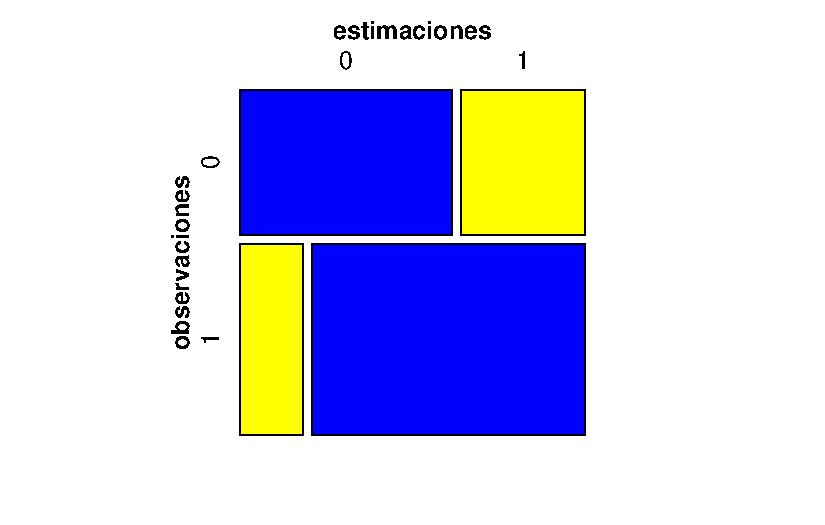
\includegraphics{cap1_files/figure-pdf/matriz_confusion Probit-1.pdf}

\begin{Shaded}
\begin{Highlighting}[]
\FunctionTok{library}\NormalTok{(gmodels)}

\FunctionTok{CrossTable}\NormalTok{(mroz}\SpecialCharTok{$}\NormalTok{inlf, predi.probit,}
           \AttributeTok{digits =} \DecValTok{2}\NormalTok{,}
           \AttributeTok{format =} \StringTok{"SPSS"}\NormalTok{,}
           \AttributeTok{prop.c =}\NormalTok{ F,}
           \AttributeTok{prop.chisq =}\NormalTok{ F,}
           \AttributeTok{prop.t =}\NormalTok{ F,}
           \AttributeTok{dnn=}\FunctionTok{c}\NormalTok{(}\StringTok{"Observado"}\NormalTok{, }\StringTok{"estimado"}\NormalTok{))}
\end{Highlighting}
\end{Shaded}

\begin{verbatim}

   Cell Contents
|-------------------------|
|                   Count |
|             Row Percent |
|-------------------------|

Total Observations in Table:  753 

             | estimado 
   Observado |        0  |        1  | Row Total | 
-------------|-----------|-----------|-----------|
           0 |      205  |      120  |      325  | 
             |    63.08% |    36.92% |    43.16% | 
-------------|-----------|-----------|-----------|
           1 |       80  |      348  |      428  | 
             |    18.69% |    81.31% |    56.84% | 
-------------|-----------|-----------|-----------|
Column Total |      285  |      468  |      753  | 
-------------|-----------|-----------|-----------|

 
\end{verbatim}

\textbf{1. Sensitividad}: \% de positivos (1) que sob clasificados como
positivos (1). para el modelo probit seria
(\(\frac{347}{428}= 81.07\%\))

\textbf{2. Especificidad}: \% negativos(0) que son clasificado como
negativops(0). . en nuestro ejemplo\_: (\(\frac{207}{325}= 63.98\%\))

\textbf{Falsos positivos:} \% de negativos (o) clasificados como
positivos (1). En nuestro ejemplo: (\(\frac{120}{325}= 36.92\%\))

\textbf{Falsos Negativos:} \% de positivos clasificados (1) como
negativos (0). en nuestro ejemplo. (\(\frac{80}{428}= 18.69\%\))

\begin{Shaded}
\begin{Highlighting}[]
\NormalTok{predi.logit }\OtherTok{\textless{}{-}} \FunctionTok{ifelse}\NormalTok{(mroz.logit}\SpecialCharTok{$}\NormalTok{fitted.values}\SpecialCharTok{\textgreater{}=}\FloatTok{0.5}\NormalTok{,}\DecValTok{1}\NormalTok{,}\DecValTok{0}\NormalTok{)}

\NormalTok{m.confu.logit}\OtherTok{\textless{}{-}} \FunctionTok{table}\NormalTok{(mroz}\SpecialCharTok{$}\NormalTok{inlf, predi.logit,}
                        \AttributeTok{dnn =} \FunctionTok{c}\NormalTok{(}\StringTok{"observaciones"}\NormalTok{, }\StringTok{"estimaciones"}\NormalTok{))}
\NormalTok{PPC.logit }\OtherTok{\textless{}{-}} \FunctionTok{data.frame}\NormalTok{(mroz}\SpecialCharTok{$}\NormalTok{inlf, predi.logit, }\FunctionTok{ifelse}\NormalTok{(mroz}\SpecialCharTok{$}\NormalTok{inlf}\SpecialCharTok{==}\NormalTok{predi.logit,}\DecValTok{1}\NormalTok{,}\DecValTok{0}\NormalTok{))}
\FunctionTok{names}\NormalTok{(PPC.logit)}\OtherTok{=}\FunctionTok{c}\NormalTok{(}\StringTok{"infl"}\NormalTok{, }\StringTok{"Valores ajustados"}\NormalTok{, }\StringTok{"PPC"}\NormalTok{)}

\FunctionTok{prop.table}\NormalTok{(}\FunctionTok{table}\NormalTok{(PPC.logit}\SpecialCharTok{$}\NormalTok{PPC))[}\DecValTok{2}\NormalTok{]}\SpecialCharTok{*}\DecValTok{100}
\end{Highlighting}
\end{Shaded}

\begin{verbatim}
       1 
73.57238 
\end{verbatim}

\begin{Shaded}
\begin{Highlighting}[]
\FunctionTok{mosaic}\NormalTok{(m.confu.logit, }\AttributeTok{shade =}\NormalTok{ T, }\AttributeTok{colorize =}\NormalTok{ T,}
       \AttributeTok{gp =} \FunctionTok{gpar}\NormalTok{(}\AttributeTok{fill =} \FunctionTok{matrix}\NormalTok{(}\FunctionTok{c}\NormalTok{(}\StringTok{"green3"}\NormalTok{, }\StringTok{"red2"}\NormalTok{, }\StringTok{"red2"}\NormalTok{, }\StringTok{"green3"}\NormalTok{),}
                               \DecValTok{2}\NormalTok{,}\DecValTok{2}\NormalTok{)))}
\end{Highlighting}
\end{Shaded}

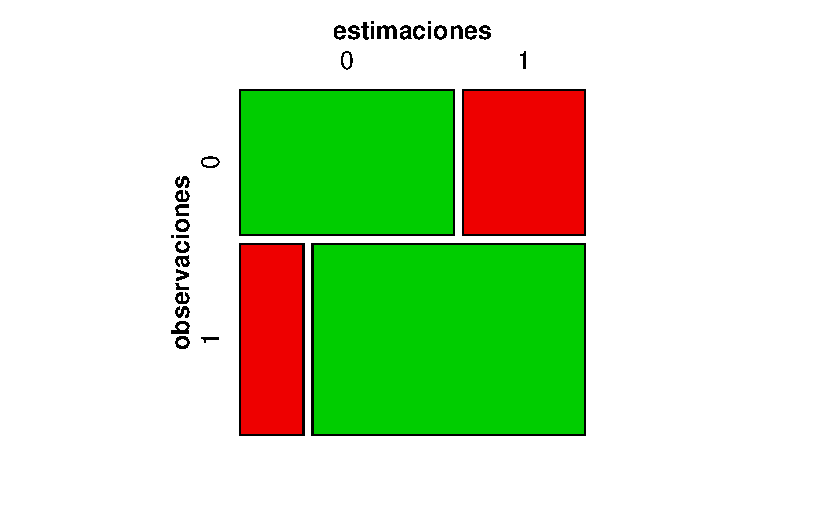
\includegraphics{cap1_files/figure-pdf/Logit PPC-1.pdf}

\begin{Shaded}
\begin{Highlighting}[]
\FunctionTok{CrossTable}\NormalTok{(mroz}\SpecialCharTok{$}\NormalTok{inlf, predi.logit,}
           \AttributeTok{digits =} \DecValTok{2}\NormalTok{,}
           \AttributeTok{format =} \StringTok{"SPSS"}\NormalTok{,}
           \AttributeTok{prop.c =}\NormalTok{ F,}
           \AttributeTok{prop.chisq =}\NormalTok{ F,}
           \AttributeTok{prop.t =}\NormalTok{ F,}
           \AttributeTok{dnn=}\FunctionTok{c}\NormalTok{(}\StringTok{"Observado"}\NormalTok{, }\StringTok{"estimado"}\NormalTok{))}
\end{Highlighting}
\end{Shaded}

\begin{verbatim}

   Cell Contents
|-------------------------|
|                   Count |
|             Row Percent |
|-------------------------|

Total Observations in Table:  753 

             | estimado 
   Observado |        0  |        1  | Row Total | 
-------------|-----------|-----------|-----------|
           0 |      207  |      118  |      325  | 
             |    63.69% |    36.31% |    43.16% | 
-------------|-----------|-----------|-----------|
           1 |       81  |      347  |      428  | 
             |    18.93% |    81.07% |    56.84% | 
-------------|-----------|-----------|-----------|
Column Total |      288  |      465  |      753  | 
-------------|-----------|-----------|-----------|

 
\end{verbatim}

Los modelos logit y probit son capaces de clasificar correctamente el
\(73.5%
\) de las observaciones cuando se emplean los datos de trabajo femenino.

\subsection{Capacidad discriminante del
modelo}\label{capacidad-discriminante-del-modelo}

\begin{Shaded}
\begin{Highlighting}[]
\FunctionTok{library}\NormalTok{(}\StringTok{"Epi"}\NormalTok{)}

\FunctionTok{ROC}\NormalTok{(}\AttributeTok{form=}\NormalTok{inlf}\SpecialCharTok{\textasciitilde{}}\NormalTok{nwifeinc}\SpecialCharTok{+}
\NormalTok{            educ}\SpecialCharTok{+}
\NormalTok{            exper}\SpecialCharTok{+}
\NormalTok{            expersq}\SpecialCharTok{+}
\NormalTok{            age}\SpecialCharTok{+}
\NormalTok{            kidslt6}\SpecialCharTok{+}
\NormalTok{            kidsge6,}
          \AttributeTok{data =}\NormalTok{ mroz)}
\end{Highlighting}
\end{Shaded}

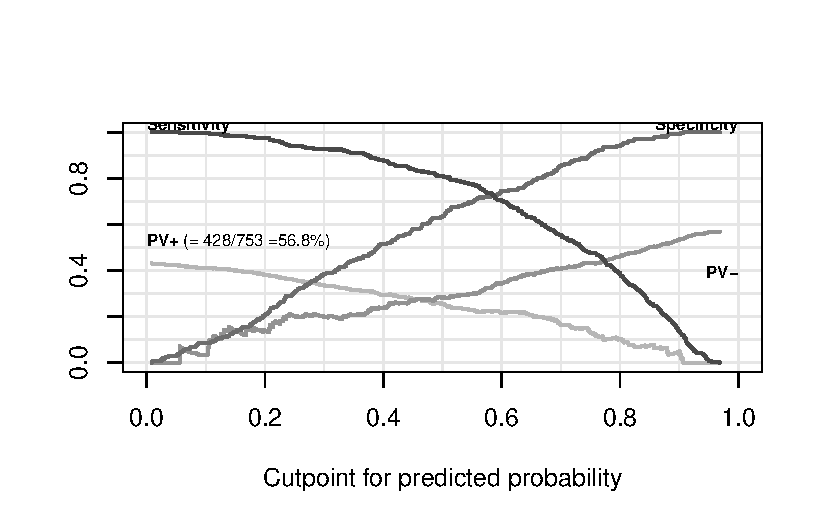
\includegraphics{cap1_files/figure-pdf/ROC-1.pdf}

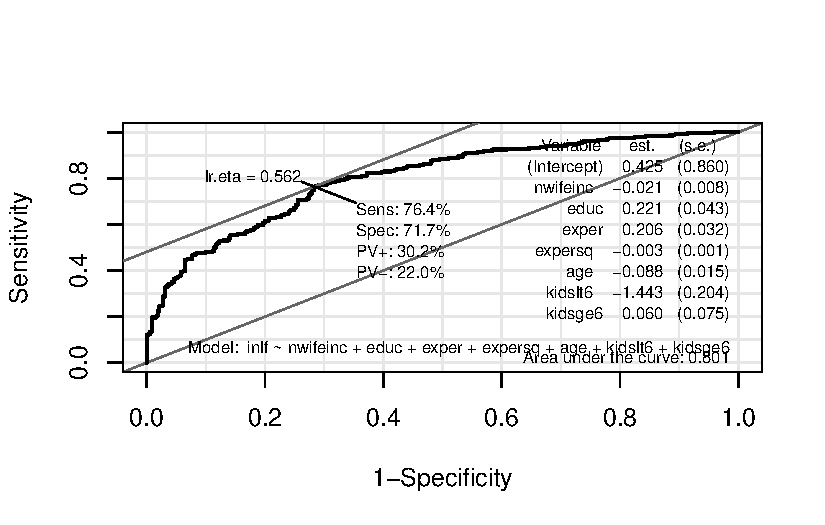
\includegraphics{cap1_files/figure-pdf/ROC-2.pdf}

\textbf{Sensibilidad}: la probabilidad de que el modelo prediga un
resultado positivo (1) para una observación cuando en realidad el
resultado es positivo (1)

\textbf{Especificidad}: La probabilidad de que el modelo prediga un
resultado negativo para una observación cuando en realidad el resultado
es negativo.

\bookmarksetup{startatroot}

\chapter{Ejercicio 17.2 del libro de
Wooldridge}\label{ejercicio-17.2-del-libro-de-wooldridge}

Sea \(grad\) una variable binaria para si un atleta colegial en una
universidad grande se graduará en cinco años. Sean \(hsGPA\)y \(SAT\) el
promedio de calificaciones de bachillerato y las puntuaciones del
\(SAT\) de admisión a la universidad, respectivamente. Sea \(study\) el
número de horas por semana que pasa un estudiante en un aula de estudio.
Suponga que, usando los datos sobre 420 atletas colegiales se obtiene el
siguiente modelo logit:

\[
\widehat{P}(grad=1|hsGPA,SAT,study)=\Lambda(-1.17+0.24hsGPA+0.00058SAT+0.073study) 
\] \[
\Lambda =\frac{exp(z)}{[1+exp(z)]}
\] Si mantiene \(hsGPA = 3.0\) y el \(SAT = 1200\), calcule la
diferencia estimada en la probabilidad de graduación para alguien que
pasa 10 horas a la semana en el aula de estudio y alguien que pasa 5
horas por semana.

\begin{Shaded}
\begin{Highlighting}[]
\NormalTok{lambda }\OtherTok{\textless{}{-}}\NormalTok{(}\SpecialCharTok{{-}}\FloatTok{1.17+0.24}\SpecialCharTok{*}\DecValTok{3}\FloatTok{+0.00058}\SpecialCharTok{*}\DecValTok{1200}\FloatTok{+0.073}\SpecialCharTok{*}\DecValTok{10}\NormalTok{)}
\NormalTok{lambda\_5 }\OtherTok{\textless{}{-}}\NormalTok{ (}\SpecialCharTok{{-}}\FloatTok{1.17+0.24}\SpecialCharTok{*}\DecValTok{3}\FloatTok{+0.00058}\SpecialCharTok{*}\DecValTok{1200}\FloatTok{+0.073}\SpecialCharTok{*}\DecValTok{5}\NormalTok{)}

\NormalTok{diferencia }\OtherTok{\textless{}{-}}\NormalTok{(}\FunctionTok{exp}\NormalTok{(lambda)}\SpecialCharTok{/}\NormalTok{(}\DecValTok{1}\SpecialCharTok{+}\FunctionTok{exp}\NormalTok{(lambda)))}\SpecialCharTok{{-}}\NormalTok{(}\FunctionTok{exp}\NormalTok{(lambda\_5)}\SpecialCharTok{/}\NormalTok{(}\DecValTok{1}\SpecialCharTok{+}\FunctionTok{exp}\NormalTok{(lambda\_5)))}
\NormalTok{diferencia}\SpecialCharTok{*}\DecValTok{100}
\end{Highlighting}
\end{Shaded}

\begin{verbatim}
[1] 7.814493
\end{verbatim}

\bookmarksetup{startatroot}

\chapter{Tareas}\label{tareas}

\begin{enumerate}
\def\labelenumi{\arabic{enumi}.}
\tightlist
\item
  Tarea: realizar todos los cálculos para el modelo de los arrestos,
  igual como se hizo en clase para los dos modelos, es decir, con y sin
  variables binarias.
\end{enumerate}

\bookmarksetup{startatroot}

\chapter{Modelo Tobit}\label{modelo-tobit}

\section{Motivación}\label{motivaciuxf3n}

Otro tipo de variable dependiente limitada es una de respuesta de
solución de esquina. La variable dependiente es cero para una fracción
no trivial \emph{representativa}, pero también existen valores de una
distribución \textbf{aproximadamente continua} a través de valores
positivos. Por ejemplo, el salario, habrá algunos individuos que ganen
cero dólares por hora y otros que ganen valores aproximadamente
continuos. Otro ejemplo, la cantidad que el individuo gasta en alcohol
cada mes. Esta variable asume un amplio rango de valores en personas
mayores a los 18 años.

\section{Especificación
matemática}\label{especificaciuxf3n-matemuxe1tica}

Sea \(y\) una variable que asume datos aproximadamente continuos en
valores estrictamente positivos, pero que asume cero con probabilidad
positiva. En este caso se podría usar un modelo lineal para \(y\). De
hecho, un modelo lineal podría ser una buena aproximación a
\(E(y|x_1,x_2,...,x_k)\) en especial para \(x_j\) cerca de los valores
promedio. Nuevamente, obtendríamos valores ajustado negativos, lo que
generaría predicciones negativas para \(y\), es decir, problemas
análogos a los del MPL. También el supuesto de que una variable
explicativa que aparece en la forma de nivel tiene un efecto parcial
constante sobre \(E(y|\mathbf{X})\) puede ser egañoso. Problablemente la
\(Var(y|\mathbf{X})\) sería no constante o heterocedástica, debido a que
la distribución de \(y\) se acumula en cero; esta claro que \(y\) no
puede tener una distribución normal condicional. Por lo tanto, al igual
que en el MPL la inferencia sólo se justifica asintóticamente.

Es importante tener un modelo que implique valores predichos no
negativos para \(y\) y, que tenga efectos parciales sensatos sobre un
amplio rango de las variables independientes. Además, algunas veces es
necesario estimar las características de la distribución de \(y\) dadas
\(x_1,...,x_k\) más alla de la expectativa condicional. El
\textbf{Modelo Tobit} es idóneo, el cual expresa la respuesta observada,
\(y\), en términos de una variable latente subyacente:

\[y^*=\beta_0+\mathbf{x\beta}+u, u|\mathbf{x}\sim Normal(0,\sigma^2)[1]\]
\[y=max(0,y^*)[2]\]

La variable latente \(y^*\) satisface los supuesto del modelo lineal
clásico, en particular tiene:

\begin{itemize}
\item
  Distribución normal
\item
  Homocedástica con una media condicional lineal
\end{itemize}

La ecuación {[}2{]} implica que la variable observable,
\(y=y^*\Leftrightarrow y^*\geq0\), caso contrario
\(y=0\Leftrightarrow y^*<0\). Debido a que \(y^*\) se distribuye como
una normal, \(y\) tiene una distribución continua a través de valores
estrictamente positivos. En particular, la densidad de \(y|\mathbf{X}\)
es la misma de \(y^*|\mathbf{X}\) para valores positivos, Además:

\[P(y=0|\mathbf{x})=P(y^*<0|\mathbf{x})=P(u<-\mathbf{x\beta}|\mathbf{x})=\\P(u|\sigma<-\mathbf{x\beta/\sigma|x})=\Phi(\mathbf{-x\beta/\sigma})=1-\Phi(\mathbf{x\beta/\sigma}) [3]\]
Notar que \(u/\sigma\sim N(0,1)\) y es independiente de \(\mathbf{x}\);
se ha absorbido el intercepto en \(\mathbf{x}\) por simplicidad
notacional. Por lo tanto, si \(\mathbf{x_i},y_i\) se extraen
aleatoriamente de la población, la densidad de \(y_i|\mathbf{x_i}\) es:

\[(2\pi\sigma^2)^{-1/2}exp[-(y-\mathbf{x_i\beta})^2/(2\sigma^2)]=(1/\sigma)\phi[(y-\mathbf{x_i\beta})/\sigma], y>0[4]\]

\[P(y_i=0|y-\mathbf{x_i})=1-\Phi(\mathbf{x_i\beta/\sigma})[5]\] Donde
\(\phi\) es la función de densidad normal estándar

De las ecuaciones {[}4{]} y {[}5{]} se obtiene la función
log-verosimilitud para cada observación \(i\):

\[\mathcal{l_i(\beta,\sigma)}=1(y_i=0)log[1-\Phi(\mathbf{x_i\beta/\sigma})]+1(y_i>0)log((1/\sigma)\phi[(y_i-\mathbf{x_i\beta})/\sigma]) [6]\]
Notese que, esto depende de \(\sigma\), la desviación estándar de \(u\),
así como de las \(\beta_j\). La log-verosimilitud para una \(n\)
aleatoria se obtiene al sumar {[}6{]}, a través de todas \(i\). Las
estimaciones de máxima verosimilitud de \(\beta\) y \(\sigma\) se
obtienen al maximizar la log-verosimilitud; esto requiere métodos
numéricos, pero el software lo realiza.

Para restricciones de exclusión múltiples es fácil usar la prueba de
\textbf{Wald} o la razón de verosimilitudes.

\section{Interpretaciones de las estimaciones
Tobit.}\label{interpretaciones-de-las-estimaciones-tobit.}

Los resultados de Tobit y MCO son casi siempre similares, lo que hace
tentador interpretar las \(\widehat{\beta}_j\) de Tobit como si fueran
estimaciones de MCO, pero se advierte que no es así de fácil.

La {[}1{]} muestra que las \(\beta_j\) miden efectos parciales de las
\(x_j\) sobre el \(E(y^*|\mathbf{x})\). La variable que se busca
explicar es \(y\), pues es el resultado observado (las horas trabajadas
o la cantidad donaciones)

De la ecuación {[}5{]} podemos obtener \(P(y=0|\mathbf{x})\), de ahi
podemos estimar \(P(y>0|\mathbf{x})\) ¿Qué pasa si se quiere estimar el
valor esperado de \(y\) en función \(\mathbf{x}\)?. En los modelos
Tobit, existe dos expectativas. La primera \(E(y|y>0,\mathbf{x})\), que
recibe el nombre de \textbf{expectativa condicional}. La segunda es
\(E(y|\mathbf{x})\), conocida como la \textbf{expectativa no
condicional}. La expectativa \(E(y|y>0,\mathbf{x})\) nos dice que, para
los valores dados de \(\mathbf{x}\), el valor esperado de \(y\) para la
subpoblación donde \(y>0\), esta expectativa se hallar con facilidades a
partir \(E(y|\mathbf{x})\):

\[E(y|\mathbf{x})=P(y>0|\mathbf{x}).E(y|y>0,\mathbf{x})=\Phi(\mathbf{x\beta}/\sigma).E(y|y>0,\mathbf{x}) [7]\]
Para obtener \(E(y|y>0,\mathbf{x})\) se puede usar un resultado para las
variables aleatorias con distribución normal: si \(z\sim Normal(0,1)\)
entonces \(E(z|z>c)=\phi(c)/[1-\Phi(c)] \forall c\) constante. Pero
\(E(y|y>0,\mathbf{x})=\mathbf{x\beta}+E(u|u>-\mathbf{x\beta})=\\\mathbf{x\beta}+\sigma E[(u/\sigma)|(u/\sigma)>-\mathbf{x\beta/\sigma}]=\\\mathbf{x\beta}+\sigma\phi_(\mathbf{x\beta}/\sigma)/\Phi(\mathbf{x\beta}/\sigma)\)

Debido a que: \(\phi(-c)=\phi(c), 1-\Phi(c)=\Phi(c)\),
\(u/\sigma\sim Normal (0,1)\) independiente de \(\mathbf{x}\). Podemos
reecribir a {[}7{]} así:

\[E(y|y>0,\mathbf{x})=\mathbf{x\beta}+\sigma\lambda(\mathbf{x\beta/\sigma})\]
Donde: \(\lambda(c)=\frac{\phi(c)}{\Phi(c)}\) recibe el nombre de la
\textbf{razón inversa de Mills}

\section{Ejemplo}\label{ejemplo}

Estimación Tobit y MCO de las horas anuales trabajas

La variables

\begin{itemize}
\item
  Dependiente (\(Y\)) son las horas anuales trabajadas por las mujeres
\item
  Variables explicativas o regresoras:
\item
  \(nwifeinc\): Salario de esposo en miles de dólares
\item
  \(educ\): años de educación
\item
  \(exper:\) años de experiencia
\item
  \(exper^2\): años de experiencia al cuadrado
\item
  \(age:\) edad de las mujeres
\item
  \(kidslt6\): Niños menores a seis años
\item
  \(kidsge6\): Niños entres 6 y 18 años
\end{itemize}

\subsection{Verificar que la variable dependiente sea de solución de
esquina}\label{verificar-que-la-variable-dependiente-sea-de-soluciuxf3n-de-esquina}

activación de paquetes

\begin{Shaded}
\begin{Highlighting}[]
\NormalTok{pacman}\SpecialCharTok{::}\FunctionTok{p\_load}\NormalTok{(wooldridge, }
\NormalTok{               dplyr, }
\NormalTok{               ggplot2, }
\NormalTok{               stargazer,}
\NormalTok{               censReg,}
\NormalTok{               AER)}
\end{Highlighting}
\end{Shaded}

\begin{Shaded}
\begin{Highlighting}[]
\NormalTok{datos }\OtherTok{\textless{}{-}} \FunctionTok{data}\NormalTok{(}\StringTok{"mroz"}\NormalTok{)}



\CommentTok{\# Histograma}
\FunctionTok{hist}\NormalTok{(mroz}\SpecialCharTok{$}\NormalTok{hours, }\AttributeTok{main =} \StringTok{"Histograma de las horas trabajadas"}\NormalTok{, }\AttributeTok{xlab =} \StringTok{"Horas trabajadas"}\NormalTok{)}
\end{Highlighting}
\end{Shaded}

\includegraphics{cap2_files/figure-pdf/unnamed-chunk-2-1.pdf}

\begin{Shaded}
\begin{Highlighting}[]
\FunctionTok{library}\NormalTok{(ggplot2)}

\FunctionTok{ggplot}\NormalTok{(}\AttributeTok{data =}\NormalTok{ mroz, }\FunctionTok{aes}\NormalTok{(}\AttributeTok{x=}\NormalTok{hours))}\SpecialCharTok{+}
  \FunctionTok{geom\_histogram}\NormalTok{(}\AttributeTok{bindwidth=}\DecValTok{10}\NormalTok{)}\SpecialCharTok{+}
  \FunctionTok{theme\_bw}\NormalTok{()}\SpecialCharTok{+}
  \FunctionTok{labs}\NormalTok{(}\AttributeTok{title =} \StringTok{"Distribución de las horas trabajas}\SpecialCharTok{\textbackslash{}n}\StringTok{ de las mujeres"}\NormalTok{)}
\end{Highlighting}
\end{Shaded}

\begin{verbatim}
Warning in geom_histogram(bindwidth = 10): Ignoring unknown parameters:
`bindwidth`
\end{verbatim}

\begin{verbatim}
`stat_bin()` using `bins = 30`. Pick better value with `binwidth`.
\end{verbatim}

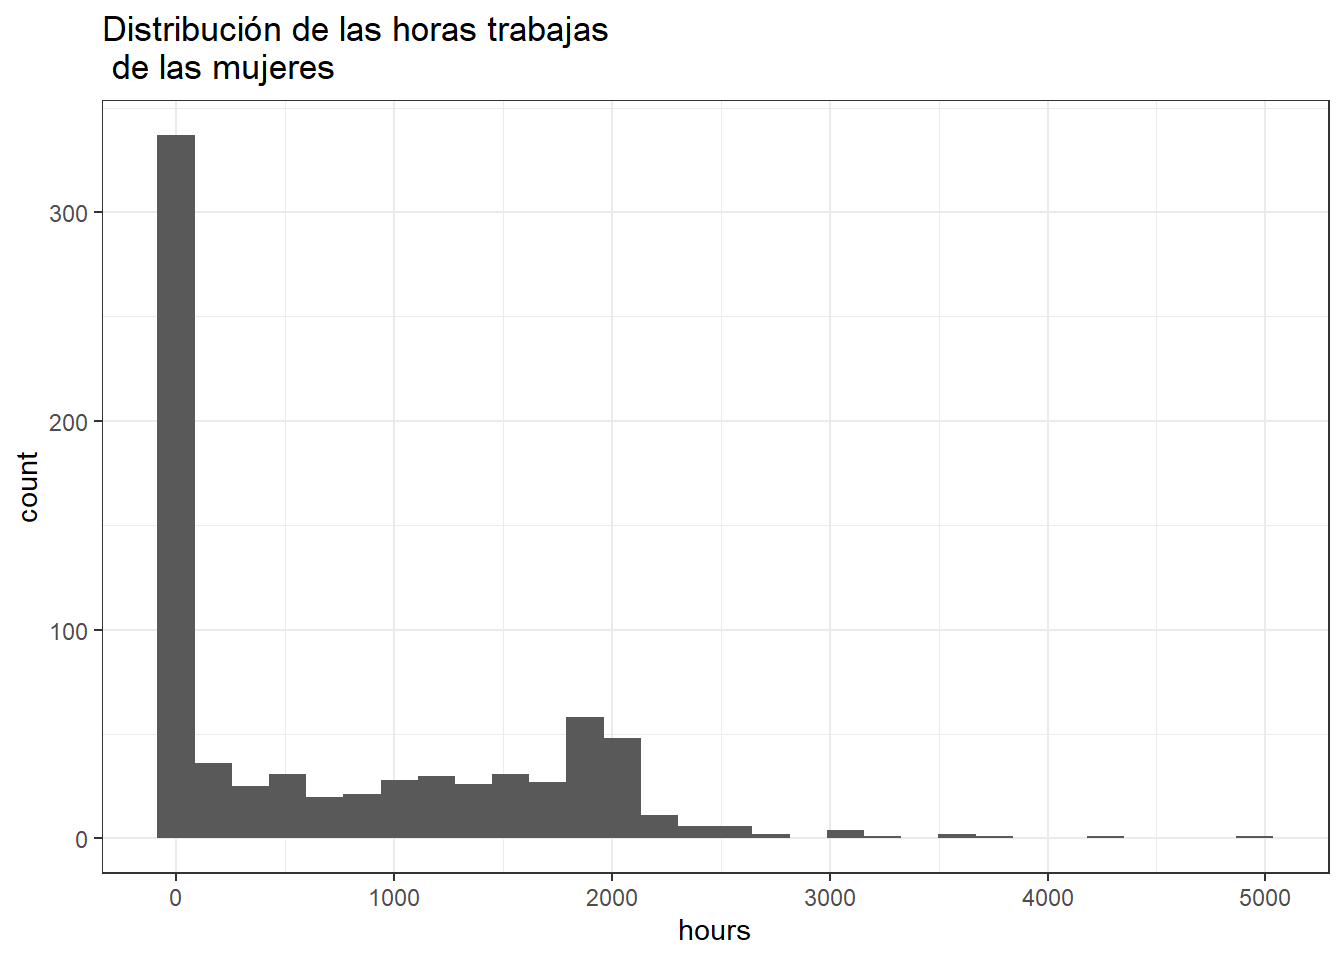
\includegraphics{cap2_files/figure-pdf/unnamed-chunk-2-2.pdf}

En el anterior histograma se puede observar que las mayor cantidad de
obervaciones se encuentran en cero, así tenemos indicios de que la
variable \(y\) es de solución de esquina, pues a además, la horas
trabajadas anuales se amplían hasta 5000 al año. Para saber la
proporcion de ceros que tiene la variable dependiente dicotomizamos
dicha variables

\begin{Shaded}
\begin{Highlighting}[]
\CommentTok{\# Transformación de la variable en binaria}
\NormalTok{mroz}\SpecialCharTok{$}\NormalTok{dico.hours }\OtherTok{\textless{}{-}} \FunctionTok{ifelse}\NormalTok{(mroz}\SpecialCharTok{$}\NormalTok{hours}\SpecialCharTok{==}\DecValTok{0}\NormalTok{,}\DecValTok{0}\NormalTok{,}\DecValTok{1}\NormalTok{)}

\CommentTok{\# Calculando el porcentaje de ceros en Y}
\FunctionTok{prop.table}\NormalTok{(}\FunctionTok{table}\NormalTok{(mroz}\SpecialCharTok{$}\NormalTok{dico.hours))}\SpecialCharTok{*}\DecValTok{100}
\end{Highlighting}
\end{Shaded}

\begin{verbatim}

       0        1 
43.16069 56.83931 
\end{verbatim}

\subsection{Usando MCO}\label{usando-mco}

Vamos a determinar las horas trabajadas al año por la mujeres, usando
MCO

\begin{Shaded}
\begin{Highlighting}[]
\NormalTok{model.mco}\OtherTok{\textless{}{-}}\FunctionTok{lm}\NormalTok{(hours}\SpecialCharTok{\textasciitilde{}}
\NormalTok{                nwifeinc}\SpecialCharTok{+}
\NormalTok{                 educ}\SpecialCharTok{+}
\NormalTok{                 exper}\SpecialCharTok{+}
\NormalTok{                 expersq}\SpecialCharTok{+}
\NormalTok{                 age}\SpecialCharTok{+}
\NormalTok{                 kidslt6}\SpecialCharTok{+}
\NormalTok{                 kidsge6,}
               \AttributeTok{data=}\NormalTok{mroz)}

\FunctionTok{library}\NormalTok{(stargazer)}

\FunctionTok{stargazer}\NormalTok{(model.mco,}
          \AttributeTok{type =} \StringTok{"text"}\NormalTok{, }
          \AttributeTok{dep.var.labels =} \StringTok{"Horas al año trabajadas"}\NormalTok{)}
\end{Highlighting}
\end{Shaded}

\begin{verbatim}

===============================================
                        Dependent variable:    
                    ---------------------------
                      Horas al año trabajadas  
-----------------------------------------------
nwifeinc                      -3.447           
                              (2.544)          
                                               
educ                         28.761**          
                             (12.955)          
                                               
exper                        65.673***         
                              (9.963)          
                                               
expersq                      -0.700**          
                              (0.325)          
                                               
age                         -30.512***         
                              (4.364)          
                                               
kidslt6                     -442.090***        
                             (58.847)          
                                               
kidsge6                       -32.779          
                             (23.176)          
                                               
Constant                   1,330.482***        
                             (270.785)         
                                               
-----------------------------------------------
Observations                    753            
R2                             0.266           
Adjusted R2                    0.259           
Residual Std. Error     750.179 (df = 745)     
F Statistic           38.495*** (df = 7; 745)  
===============================================
Note:               *p<0.1; **p<0.05; ***p<0.01
\end{verbatim}

\begin{Shaded}
\begin{Highlighting}[]
\CommentTok{\# Si la variable "y" ajustada tiene valores menores que cero, significa que no es un buen ajuste}

\FunctionTok{summary}\NormalTok{(model.mco}\SpecialCharTok{$}\NormalTok{fitted.values)}
\end{Highlighting}
\end{Shaded}

\begin{verbatim}
   Min. 1st Qu.  Median    Mean 3rd Qu.    Max. 
 -719.8   417.5   737.7   740.6  1093.1  1614.7 
\end{verbatim}

\begin{Shaded}
\begin{Highlighting}[]
\FunctionTok{summary}\NormalTok{(mroz}\SpecialCharTok{$}\NormalTok{hours)}
\end{Highlighting}
\end{Shaded}

\begin{verbatim}
   Min. 1st Qu.  Median    Mean 3rd Qu.    Max. 
    0.0     0.0   288.0   740.6  1516.0  4950.0 
\end{verbatim}

Como me arroja valores negativos ajustados, significa que el MCO no esta
ajustando de forma adecuada a la variable \(y\) de solución de esquina.
Además, el efecto es constante. Esto me siguiere que se debe usar un
modelo Tobit para ajustar una variable de solución de esquina.

\subsection{Modelo Tobit}\label{modelo-tobit-1}

Por lo antes mencionado, ajustamos a la variable \emph{hours} con un
modelo \textbf{Tobit}

Verificar el cumpliendo de la variable \emph{hours} para usar un modelo
Tobit.

\begin{Shaded}
\begin{Highlighting}[]
\CommentTok{\# Porcentaje de ceros en la variable hours}

\NormalTok{mroz}\SpecialCharTok{$}\NormalTok{dico }\OtherTok{\textless{}{-}} \FunctionTok{ifelse}\NormalTok{(mroz}\SpecialCharTok{$}\NormalTok{hours}\SpecialCharTok{==}\DecValTok{0}\NormalTok{,}\DecValTok{0}\NormalTok{,}\DecValTok{1}\NormalTok{)}
\FunctionTok{prop.table}\NormalTok{(}\FunctionTok{table}\NormalTok{(mroz}\SpecialCharTok{$}\NormalTok{dico))}\SpecialCharTok{*}\DecValTok{100}
\end{Highlighting}
\end{Shaded}

\begin{verbatim}

       0        1 
43.16069 56.83931 
\end{verbatim}

En este ejemplo aproximadamente el 43\% de los datos de \emph{hours} son
cero y el resto datos aproximadamente continuos

Procedemos a ajustar un modelo Tobit

\begin{Shaded}
\begin{Highlighting}[]
\NormalTok{modelo.tobit }\OtherTok{\textless{}{-}} \FunctionTok{censReg}\NormalTok{(hours}\SpecialCharTok{\textasciitilde{}}
\NormalTok{                nwifeinc}\SpecialCharTok{+}
\NormalTok{                 educ}\SpecialCharTok{+}
\NormalTok{                 exper}\SpecialCharTok{+}
\NormalTok{                 expersq}\SpecialCharTok{+}
\NormalTok{                 age}\SpecialCharTok{+}
\NormalTok{                 kidslt6}\SpecialCharTok{+}
\NormalTok{                 kidsge6,}
               \AttributeTok{data=}\NormalTok{mroz,}
               \AttributeTok{left =} \DecValTok{0}\NormalTok{)}

\NormalTok{modelo.tobit2 }\OtherTok{\textless{}{-}} \FunctionTok{tobit}\NormalTok{(hours}\SpecialCharTok{\textasciitilde{}}
\NormalTok{                nwifeinc}\SpecialCharTok{+}
\NormalTok{                 educ}\SpecialCharTok{+}
\NormalTok{                 exper}\SpecialCharTok{+}
\NormalTok{                 expersq}\SpecialCharTok{+}
\NormalTok{                 age}\SpecialCharTok{+}
\NormalTok{                 kidslt6}\SpecialCharTok{+}
\NormalTok{                 kidsge6,}
               \AttributeTok{data=}\NormalTok{mroz)}
\end{Highlighting}
\end{Shaded}

Una vez, ejecutadas las dos regresiones (MCO y Tobit) las ponemos a
comparación, de tal forma que, se replique la \textbf{Tabla 17.2B} del
libro de Wooldridge (2010)

\begin{Shaded}
\begin{Highlighting}[]
\FunctionTok{stargazer}\NormalTok{(model.mco, }
\NormalTok{          modelo.tobit, }
\NormalTok{          modelo.tobit2 ,}
          \AttributeTok{digits =} \DecValTok{2}\NormalTok{,}
          \AttributeTok{type =} \StringTok{"text"}\NormalTok{,}
          \AttributeTok{df=}\NormalTok{F,}
          \AttributeTok{title =} \StringTok{"Estimación Tobit y MCO de las horas anuales trabajas"}\NormalTok{,}
          \AttributeTok{dep.var.labels =} \StringTok{"Variable dependiente: horas anuales trabajadas"}\NormalTok{,}
          \AttributeTok{header =}\NormalTok{ F,}
          \AttributeTok{column.labels =} \FunctionTok{c}\NormalTok{(}\StringTok{"MCO"}\NormalTok{, }\StringTok{"Tobit"}\NormalTok{, }\StringTok{"Tobit2"}\NormalTok{),}
          \AttributeTok{model.names =}\NormalTok{ F)}
\end{Highlighting}
\end{Shaded}

\begin{verbatim}

Estimación Tobit y MCO de las horas anuales trabajas
====================================================================
                                  Dependent variable:               
                    ------------------------------------------------
                     Variable dependiente: horas anuales trabajadas 
                          MCO             Tobit          Tobit2     
                          (1)              (2)             (3)      
--------------------------------------------------------------------
nwifeinc                 -3.45           -8.81**         -8.81**    
                         (2.54)          (4.46)          (4.46)     
                                                                    
educ                    28.76**         80.65***        80.65***    
                        (12.95)          (21.58)         (21.58)    
                                                                    
exper                   65.67***        131.56***       131.56***   
                         (9.96)          (17.28)         (17.28)    
                                                                    
expersq                 -0.70**         -1.86***        -1.86***    
                         (0.32)          (0.54)          (0.54)     
                                                                    
age                    -30.51***        -54.41***       -54.41***   
                         (4.36)          (7.42)          (7.42)     
                                                                    
kidslt6                -442.09***      -894.02***      -894.02***   
                        (58.85)         (111.88)        (111.88)    
                                                                    
kidsge6                  -32.78          -16.22          -16.22     
                        (23.18)          (38.64)         (38.64)    
                                                                    
logSigma                                 7.02***                    
                                         (0.04)                     
                                                                    
Constant              1,330.48***       965.31**        965.31**    
                        (270.78)        (446.44)        (446.44)    
                                                                    
--------------------------------------------------------------------
Observations              753              753             753      
R2                        0.27                                      
Adjusted R2               0.26                                      
Log Likelihood                          -3,819.09       -3,819.09   
Akaike Inf. Crit.                       7,656.19                    
Bayesian Inf. Crit.                     7,697.81                    
Residual Std. Error      750.18                                     
F Statistic             38.50***                                    
Wald Test                                               253.86***   
====================================================================
Note:                                    *p<0.1; **p<0.05; ***p<0.01
\end{verbatim}

Si quiero hacer comparables las estimaciones Tobit con MCO se debe
multiplicar por el factor de ajuste. El factor escalar \textbf{EPP}
\(n^{-1}\Sigma_{i=1}^n\Phi(\mathbf{x_i\hat{\beta}}/\hat{\sigma})\)
resulta que es aproximadamente de 0.589. Por ejemplo, \emph{educ} por
0.589 se obtiene \(0.589(80.65)\approx47.50\), por lo tanto, si una
mujer aumenta un año a su educación, en promedio se sumara 47.5 horas de
trabajo, esto es mayor al MCO, que es de 28.76. Se podría usar otro
escalar a partir de los valores promedio de todas las variables
explicativas, entonces se calcula el \emph{EPA}
\(\Phi(\mathbf{\bar{x}_i\hat{\beta}}/\hat{\sigma})\), es aproximadamente
0.645

\subsubsection{Efecto marginal}\label{efecto-marginal}

A continuación, uso el comando \emph{margEff()} para encontrar los
efectos marginales de la estimación Tobit

\begin{Shaded}
\begin{Highlighting}[]
\FunctionTok{summary}\NormalTok{(}\FunctionTok{margEff}\NormalTok{(modelo.tobit))}
\end{Highlighting}
\end{Shaded}

\begin{verbatim}
         Marg. Eff. Std. Error t value  Pr(>|t|)    
nwifeinc   -5.32644    2.69073 -1.9796 0.0481217 *  
educ       48.73409   12.96341  3.7594 0.0001837 ***
exper      79.50423   10.30497  7.7151 3.886e-14 ***
expersq    -1.12651    0.32326 -3.4848 0.0005213 ***
age       -32.87692    4.45770 -7.3753 4.383e-13 ***
kidslt6  -540.25683   66.62393 -8.1091 2.220e-15 ***
kidsge6    -9.80053   23.36134 -0.4195 0.6749580    
---
Signif. codes:  0 '***' 0.001 '**' 0.01 '*' 0.05 '.' 0.1 ' ' 1
\end{verbatim}

\textbf{Interpretaciones}

\begin{itemize}
\tightlist
\item
  Si el salario del esposo aumenta en 1000 dólares al año, las horas de
  trabajo de la mujer disminuyen en 5.32 horas. El mayor efecto, que es
  altamente significativo, sigue siendo el aumento de niños pequeños,
  pues en promedio, si se aumenta un infante menor a seis años las horas
  de trabajo decrecen en 540 horas al año.
\end{itemize}

\subsection{No linealidad del modelo
Tobit}\label{no-linealidad-del-modelo-tobit}

\begin{Shaded}
\begin{Highlighting}[]
\NormalTok{mod.stobit }\OtherTok{\textless{}{-}} \FunctionTok{censReg}\NormalTok{(hours}\SpecialCharTok{\textasciitilde{}}\NormalTok{kidslt6 , }
                      \AttributeTok{left =} \DecValTok{0}\NormalTok{,}
                      \AttributeTok{data=}\NormalTok{mroz)}
\NormalTok{mod.Smco }\OtherTok{\textless{}{-}} \FunctionTok{lm}\NormalTok{(hours}\SpecialCharTok{\textasciitilde{}}\NormalTok{kidslt6, }
               \AttributeTok{data=}\NormalTok{mroz)}

\FunctionTok{stargazer}\NormalTok{(mod.stobit, }\AttributeTok{type =} \StringTok{"text"}\NormalTok{)}
\end{Highlighting}
\end{Shaded}

\begin{verbatim}

===============================================
                        Dependent variable:    
                    ---------------------------
                               hours           
-----------------------------------------------
kidslt6                     -774.751***        
                             (116.086)         
                                               
logSigma                     7.191***          
                              (0.038)          
                                               
Constant                    489.522***         
                             (59.105)          
                                               
-----------------------------------------------
Observations                    753            
Log Likelihood              -3,930.753         
Akaike Inf. Crit.            7,867.505         
Bayesian Inf. Crit.          7,881.377         
===============================================
Note:               *p<0.1; **p<0.05; ***p<0.01
\end{verbatim}

\begin{Shaded}
\begin{Highlighting}[]
\CommentTok{\# Añadiendo la curva de regresión Tobit}

\NormalTok{x }\OtherTok{\textless{}{-}} \FunctionTok{seq}\NormalTok{(}\DecValTok{0}\NormalTok{,}\DecValTok{4}\NormalTok{, }\FloatTok{0.5}\NormalTok{)}

\NormalTok{y }\OtherTok{\textless{}{-}} \FunctionTok{pnorm}\NormalTok{((}\FunctionTok{coef}\NormalTok{(mod.stobit)[}\DecValTok{1}\NormalTok{]}\SpecialCharTok{+}\FunctionTok{coef}\NormalTok{(mod.stobit)[}\DecValTok{2}\NormalTok{]}\SpecialCharTok{*}\NormalTok{x)}\SpecialCharTok{/}\FunctionTok{exp}\NormalTok{(}\FunctionTok{coef}\NormalTok{(mod.stobit)[}\DecValTok{3}\NormalTok{]))}\SpecialCharTok{*}\NormalTok{(}\FunctionTok{coef}\NormalTok{(mod.stobit)[}\DecValTok{1}\NormalTok{]}\SpecialCharTok{+}\FunctionTok{coef}\NormalTok{(mod.stobit)[}\DecValTok{2}\NormalTok{]}\SpecialCharTok{*}\NormalTok{x)}\SpecialCharTok{+}\FunctionTok{exp}\NormalTok{(}\FunctionTok{coef}\NormalTok{(mod.stobit)[}\DecValTok{3}\NormalTok{])}\SpecialCharTok{*}\FunctionTok{dnorm}\NormalTok{((}\FunctionTok{coef}\NormalTok{(mod.stobit)[}\DecValTok{1}\NormalTok{]}\SpecialCharTok{+}\FunctionTok{coef}\NormalTok{(mod.stobit)[}\DecValTok{2}\NormalTok{]}\SpecialCharTok{*}\NormalTok{x)}\SpecialCharTok{/}\FunctionTok{exp}\NormalTok{(}\FunctionTok{coef}\NormalTok{(mod.stobit)[}\DecValTok{3}\NormalTok{]))}

\FunctionTok{plot}\NormalTok{(}\AttributeTok{x=}\NormalTok{x,}
     \AttributeTok{y=}\NormalTok{y,}
     \AttributeTok{xlab =} \StringTok{"Niños menores a seis años"}\NormalTok{,}
     \AttributeTok{ylab=}\StringTok{"Horas trabajadas al año"}\NormalTok{,}
     \AttributeTok{col=}\StringTok{"steelblue"}\NormalTok{,}
     \AttributeTok{main=}\StringTok{"Modelo Tobit para la relación niños pequeños y horas trabajadas de una mujer"}\NormalTok{, }
     \AttributeTok{type=}\StringTok{"l"}\NormalTok{)}

\FunctionTok{abline}\NormalTok{(mod.Smco, }\AttributeTok{col=}\StringTok{"red"}\NormalTok{)}
\end{Highlighting}
\end{Shaded}

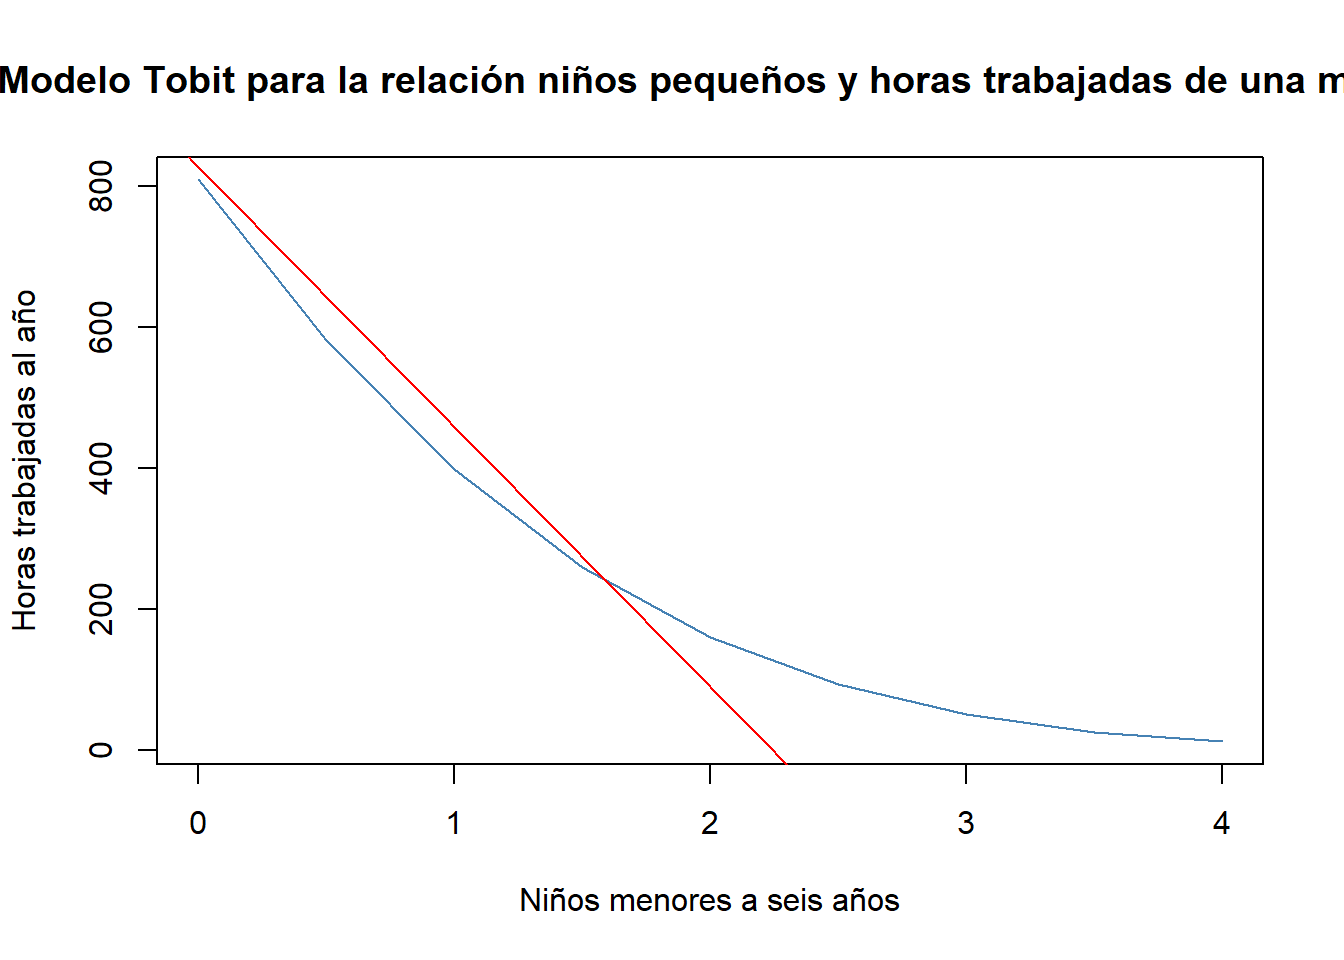
\includegraphics{cap2_files/figure-pdf/unnamed-chunk-5-1.pdf}

En el gráfico anterior podemos observar que añadir un niño menor a seis
años hace que se reduzca las horas dedicadas al trabajo. Sin embargo, en
la linea azul del modelo Tobit la reducción de horas es decreciente a
medida que se tiene más hijos pequeños, en el MCO (linea de color rojo),
la reducción de las horas trabajadas es la misma con el aparecimiento de
menor a seis años. Es decir, no importa si pasas de cero hijo a a uno
hijo o de 3 a 4, la reducción de las horas trabajadas es la misma. No
esta tomando en cuenta el aprendizaje de la madre con cada nuevo hijo.

\subsubsection{Evaluación informal del modelo Tobit {[}Problemas de
especificación{]}}\label{evaluaciuxf3n-informal-del-modelo-tobit-problemas-de-especificaciuxf3n}

\begin{Shaded}
\begin{Highlighting}[]
\NormalTok{probit.tobit }\OtherTok{\textless{}{-}}\FunctionTok{glm}\NormalTok{(dico.hours}\SpecialCharTok{\textasciitilde{}}
\NormalTok{                nwifeinc}\SpecialCharTok{+}
\NormalTok{                 educ}\SpecialCharTok{+}
\NormalTok{                 exper}\SpecialCharTok{+}
\NormalTok{                 expersq}\SpecialCharTok{+}
\NormalTok{                 age}\SpecialCharTok{+}
\NormalTok{                 kidslt6}\SpecialCharTok{+}
\NormalTok{                 kidsge6,}
               \AttributeTok{data=}\NormalTok{mroz,}
               \AttributeTok{family =} \FunctionTok{binomial}\NormalTok{(}\AttributeTok{link =} \StringTok{"probit"}\NormalTok{)) }

\FunctionTok{stargazer}\NormalTok{(probit.tobit,}
          \AttributeTok{type =} \StringTok{"text"}\NormalTok{,}
          \AttributeTok{title =} \StringTok{"Estimación Tobit y MCO de las horas anuales trabajas"}\NormalTok{,}
          \AttributeTok{dep.var.labels =} \StringTok{"Variable dependiente: horas anuales trabajadas 0 y 1"}\NormalTok{)}
\end{Highlighting}
\end{Shaded}

\begin{verbatim}

Estimación Tobit y MCO de las horas anuales trabajas
======================================================================
                                  Dependent variable:                 
                  ----------------------------------------------------
                  Variable dependiente: horas anuales trabajadas 0 y 1
----------------------------------------------------------------------
nwifeinc                                -0.012**                      
                                        (0.005)                       
                                                                      
educ                                    0.131***                      
                                        (0.025)                       
                                                                      
exper                                   0.123***                      
                                        (0.019)                       
                                                                      
expersq                                -0.002***                      
                                        (0.001)                       
                                                                      
age                                    -0.053***                      
                                        (0.008)                       
                                                                      
kidslt6                                -0.868***                      
                                        (0.118)                       
                                                                      
kidsge6                                  0.036                        
                                        (0.044)                       
                                                                      
Constant                                 0.270                        
                                        (0.508)                       
                                                                      
----------------------------------------------------------------------
Observations                              753                         
Log Likelihood                          -401.302                      
Akaike Inf. Crit.                       818.604                       
======================================================================
Note:                                      *p<0.1; **p<0.05; ***p<0.01
\end{verbatim}

Luego procedemos a usar los coeficientes para la comparación entre el
modelo Probit y el Tobit, el objetivo es evaluar la validez del modelo
Tobit.

\begin{Shaded}
\begin{Highlighting}[]
\NormalTok{z }\OtherTok{\textless{}{-}} \FunctionTok{coef}\NormalTok{(probit.tobit)}
\NormalTok{m }\OtherTok{\textless{}{-}} \FunctionTok{coef}\NormalTok{(modelo.tobit)}

\NormalTok{comparacion }\OtherTok{\textless{}{-}} \FunctionTok{data.frame}\NormalTok{(z, (m[}\DecValTok{1}\SpecialCharTok{:}\DecValTok{8}\NormalTok{])}\SpecialCharTok{/}\FunctionTok{exp}\NormalTok{(m[}\DecValTok{9}\NormalTok{]), z}\SpecialCharTok{{-}}\NormalTok{(m[}\DecValTok{1}\SpecialCharTok{:}\DecValTok{8}\NormalTok{])}\SpecialCharTok{/}\FunctionTok{exp}\NormalTok{(m[}\DecValTok{9}\NormalTok{]))}
\FunctionTok{names}\NormalTok{(comparacion) }\OtherTok{\textless{}{-}} \FunctionTok{c}\NormalTok{(}\StringTok{"probit"}\NormalTok{, }\StringTok{"beta/sigma"}\NormalTok{, }\StringTok{"diferencia"}\NormalTok{)}
\NormalTok{comparacion}
\end{Highlighting}
\end{Shaded}

\begin{verbatim}
                  probit   beta/sigma   diferencia
(Intercept)  0.270073573  0.860326776 -0.590253203
nwifeinc    -0.012023637 -0.007855680 -0.004167957
educ         0.130903969  0.071875266  0.059028703
exper        0.123347168  0.117256469  0.006090698
expersq     -0.001887067 -0.001661427 -0.000225640
age         -0.052852442 -0.048488379 -0.004364063
kidslt6     -0.868324680 -0.796795431 -0.071529248
kidsge6      0.036005611 -0.014454263  0.050459873
\end{verbatim}

Tobit de \emph{nwifeinc} entre \(\widehat{\sigma}=1122.02\), se obtuvo
\(-8.81/1122.02=-0.0079\); el coeficiente probit de \emph{nwifein} es de
cerca de \(-0.012\), lo cual es diferente, pero no de forma drástica. En
\emph{kidslt6}, el coeficiente estimado entre \(\widehat{\sigma}\) es de
cerca de \(-0.797\), en comparación con la estimación probit de
\(-0.868\). De nuevo, ésta no es una diferencia enorme, pero indica que
tener niños pequeños tiene un efecto mayor sobre la decisión inicial de
participar en la fuerza laboral que sobre cuántas horas elige trabajar
una mujer una vez que está en dicha fuerza. (Tobit promedia de forma
efectiva estos dos efectos.) No se sabe si los efectos son
estadísticamente diferentes, pero son del mismo orden de magnitud.

Por lo tanto, se podría decir que el modelo Tobit es adecuado, parar
ajustar a la variable \emph{hours}

¿Qué sucede si se concluye que el modelo Tobit es inadecuado? Existen
modelos, que suelen conocerse como modelos de \textbf{dos partes} o
\textbf{de obstáculos}, que se pueden usar cuando Tobit es inadecuado

\bookmarksetup{startatroot}

\chapter{Modelo Poisson}\label{modelo-poisson}

\section{Introducción y
motivación}\label{introducciuxf3n-y-motivaciuxf3n}

Una tercera clase de variable dependiente no negativa es una
\textbf{variable de conteo}, que puede asumir valores enteros no
negativos: \([0,1,2,...]\), específicamente los que nos interesa son los
casos en los que \(y\) asume pocos valores, incluido el cero. Ejemplos:

\begin{itemize}
\item
  El número de medallas que puede obtener un deportista en una
  olimpiada,
\item
  El número de hijos que tiene una mujer
\item
  El número de publicaciones al año de un científico
\end{itemize}

Al igual que las respuestas, binaria y Tobit, un modelo lineal para
\(E(y|x_1,x_2,...,x_k)\), quizá no proporciona el mejor ajuste a lo
largo de todos los valores de las variables explicativas. Sin embargo,
es informativo comenzar con un modelo lineal.

Como en un modelo \textbf{Tobit} no se puede obtener el logaritmo de una
variable de conteo que asume valores de cero. Un método útil es modelar
el valor esperado como una función exponencial:

\[E(y|x_1,x_2,...,x_k)=exp(\beta_0+\beta_1x_1+...+\beta_kx_k)\ [1]\]

\begin{Shaded}
\begin{Highlighting}[]
\NormalTok{pacman}\SpecialCharTok{::}\FunctionTok{p\_load}\NormalTok{(wooldridge, }
\NormalTok{               stargazer, }
\NormalTok{               tidyverse)}
\end{Highlighting}
\end{Shaded}

\subsection{Recordatorio}\label{recordatorio}

\begin{Shaded}
\begin{Highlighting}[]
\FunctionTok{data}\NormalTok{(}\StringTok{"wage1"}\NormalTok{, }\AttributeTok{package =} \StringTok{"wooldridge"}\NormalTok{)}

\CommentTok{\#Modelo lineal}

\NormalTok{salario.lm}\OtherTok{\textless{}{-}}\FunctionTok{lm}\NormalTok{(wage}\SpecialCharTok{\textasciitilde{}}\NormalTok{educ,}
\NormalTok{               wage1)}

\FunctionTok{library}\NormalTok{(stargazer)}

\FunctionTok{stargazer}\NormalTok{(salario.lm, }
          \AttributeTok{type =} \StringTok{"text"}\NormalTok{)}
\end{Highlighting}
\end{Shaded}

\begin{verbatim}

===============================================
                        Dependent variable:    
                    ---------------------------
                               wage            
-----------------------------------------------
educ                         0.541***          
                              (0.053)          
                                               
Constant                      -0.905           
                              (0.685)          
                                               
-----------------------------------------------
Observations                    526            
R2                             0.165           
Adjusted R2                    0.163           
Residual Std. Error      3.378 (df = 524)      
F Statistic          103.363*** (df = 1; 524)  
===============================================
Note:               *p<0.1; **p<0.05; ***p<0.01
\end{verbatim}

\begin{Shaded}
\begin{Highlighting}[]
\CommentTok{\# Gráfica de la relación salario y la educación}

\FunctionTok{plot}\NormalTok{(wage}\SpecialCharTok{\textasciitilde{}}\NormalTok{educ, }
\NormalTok{     wage1,}
     \AttributeTok{pch=}\DecValTok{20}\NormalTok{,}
     \AttributeTok{col=}\StringTok{"steelblue"}\NormalTok{,}
     \AttributeTok{ylab =} \StringTok{"Salario en USD por hora"}\NormalTok{,}
     \AttributeTok{xlab=}\StringTok{"años de educación"}\NormalTok{,}
     \AttributeTok{main=}\StringTok{"La relación entre el salario y la educación"}\NormalTok{)}

\FunctionTok{abline}\NormalTok{(}\DecValTok{0}\NormalTok{,}\DecValTok{0}\NormalTok{)}

\FunctionTok{abline}\NormalTok{(salario.lm, }
       \AttributeTok{lw=}\DecValTok{2}\NormalTok{,}
       \AttributeTok{col=}\StringTok{"red"}\NormalTok{)}
\end{Highlighting}
\end{Shaded}

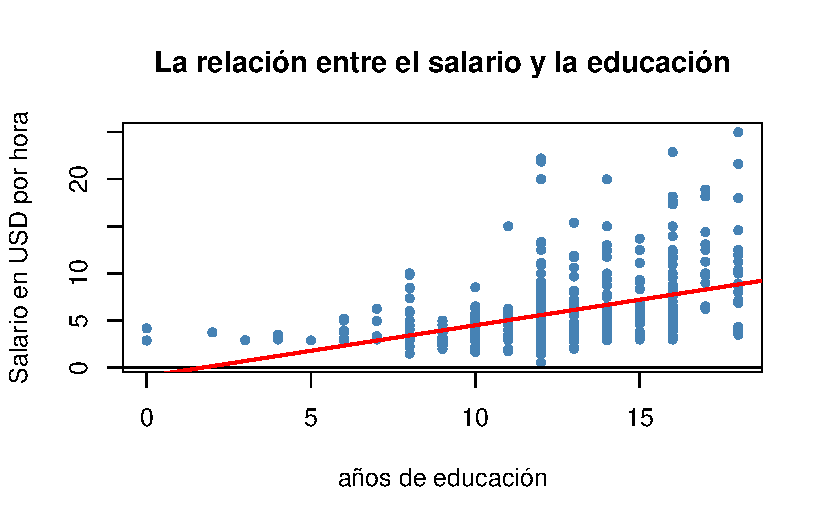
\includegraphics{cap3_files/figure-pdf/no-lineal-1.pdf}

\begin{Shaded}
\begin{Highlighting}[]
\FunctionTok{plot}\NormalTok{(}\AttributeTok{y=}\NormalTok{wage1}\SpecialCharTok{$}\NormalTok{wage,}
     \AttributeTok{x=}\NormalTok{wage1}\SpecialCharTok{$}\NormalTok{educ,}
     \AttributeTok{col=}\StringTok{"blue"}\NormalTok{,}
     \AttributeTok{pch=}\DecValTok{19}\NormalTok{,}
     \AttributeTok{xlab=}\StringTok{"Años de educación"}\NormalTok{,}
     \AttributeTok{ylab=}\StringTok{"Salario en USD/hora"}\NormalTok{)}
\end{Highlighting}
\end{Shaded}

\includegraphics{cap3_files/figure-pdf/unnamed-chunk-2-1.pdf}

\textbf{Interpretaciones}

\begin{itemize}
\tightlist
\item
  Un aumento de un año de educación, esta asociado en promedio a un
  incremento en el salario de 54 centavos por cada trabajada.
\end{itemize}

Es decir que la forma funcional al parecer, es la siguiente:

\[wage=exp(\beta_0+\beta_1educ+u)\ [2]\]

La ecuación {[}2{]} no es lineal en los parámetros, para usar el modelo
de regresión se usa un cambio usando la función logarítmica, tenemos:

\[log(wage)=\beta_0+\beta_1educ+u\]

\begin{Shaded}
\begin{Highlighting}[]
\NormalTok{log.lin}\OtherTok{\textless{}{-}}\FunctionTok{lm}\NormalTok{(}\FunctionTok{log}\NormalTok{(wage)}\SpecialCharTok{\textasciitilde{}}\NormalTok{educ,}
\NormalTok{            wage1)}
\FunctionTok{stargazer}\NormalTok{(log.lin, }
          \AttributeTok{type =} \StringTok{"text"}\NormalTok{)}
\end{Highlighting}
\end{Shaded}

\begin{verbatim}

===============================================
                        Dependent variable:    
                    ---------------------------
                             log(wage)         
-----------------------------------------------
educ                         0.083***          
                              (0.008)          
                                               
Constant                     0.584***          
                              (0.097)          
                                               
-----------------------------------------------
Observations                    526            
R2                             0.186           
Adjusted R2                    0.184           
Residual Std. Error      0.480 (df = 524)      
F Statistic          119.582*** (df = 1; 524)  
===============================================
Note:               *p<0.1; **p<0.05; ***p<0.01
\end{verbatim}

\textbf{Intepretación}

\begin{Shaded}
\begin{Highlighting}[]
\FunctionTok{exp}\NormalTok{(}\FunctionTok{coef}\NormalTok{(log.lin)[}\DecValTok{1}\NormalTok{])}
\end{Highlighting}
\end{Shaded}

\begin{verbatim}
(Intercept) 
   1.792789 
\end{verbatim}

\begin{itemize}
\item
  \(e^{0.584}=1.79\) Si no hay cambios en la educación, se predice un
  ingreso promedio por hora trabajada de 1.79 USD
\item
  Un aumento de un año en la educación esta asociado a un incremento de
  8.3\% en el salario por hora trabajada
\end{itemize}

\begin{Shaded}
\begin{Highlighting}[]
\CommentTok{\# Gráfica de la relación salario y la educación}

\FunctionTok{plot}\NormalTok{(}\FunctionTok{log}\NormalTok{(wage)}\SpecialCharTok{\textasciitilde{}}\NormalTok{educ, }
\NormalTok{     wage1,}
     \AttributeTok{pch=}\DecValTok{20}\NormalTok{,}
     \AttributeTok{col=}\StringTok{"steelblue"}\NormalTok{,}
     \AttributeTok{ylab =} \StringTok{"Salario en USD por hora"}\NormalTok{,}
     \AttributeTok{xlab=}\StringTok{"años de educación"}\NormalTok{,}
     \AttributeTok{main=}\StringTok{"La relación entre el salario y la educación"}\NormalTok{)}


\FunctionTok{abline}\NormalTok{(log.lin,}
       \AttributeTok{lw=}\DecValTok{2}\NormalTok{,}
       \AttributeTok{col=}\StringTok{"green"}\NormalTok{)}

\FunctionTok{abline}\NormalTok{(salario.lm,}
       \AttributeTok{col=}\StringTok{"red"}\NormalTok{,}
       \AttributeTok{lwd=}\DecValTok{2}\NormalTok{)}

\FunctionTok{abline}\NormalTok{(}\DecValTok{0}\NormalTok{,}\DecValTok{0}\NormalTok{)}
\end{Highlighting}
\end{Shaded}

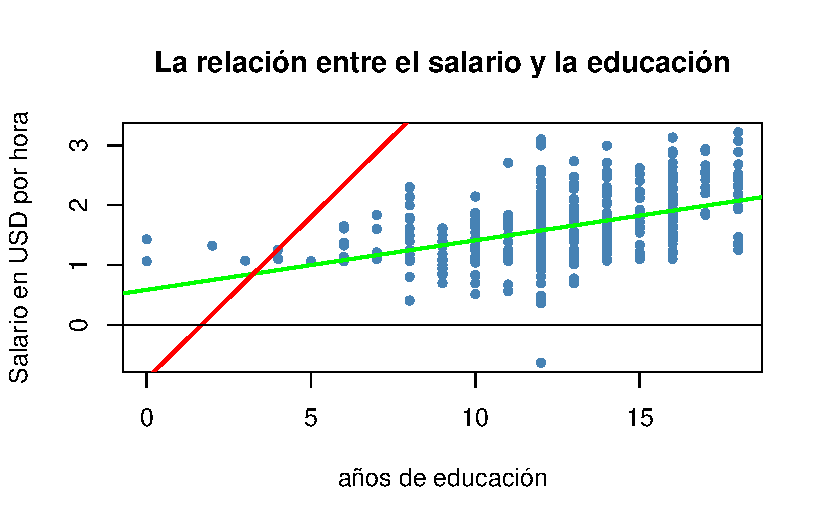
\includegraphics{cap3_files/figure-pdf/grafica-1.pdf}

\subsection{Otro ejemplo}\label{otro-ejemplo}

\begin{Shaded}
\begin{Highlighting}[]
\FunctionTok{data}\NormalTok{(}\StringTok{"CASchools"}\NormalTok{, }\AttributeTok{package =} \StringTok{"AER"}\NormalTok{)}

\NormalTok{CASchools}\SpecialCharTok{$}\NormalTok{Notas}\OtherTok{\textless{}{-}}\NormalTok{(CASchools}\SpecialCharTok{$}\NormalTok{read}\SpecialCharTok{+}\NormalTok{CASchools}\SpecialCharTok{$}\NormalTok{math)}\SpecialCharTok{/}\DecValTok{2}

\NormalTok{lineal.model}\OtherTok{\textless{}{-}}\FunctionTok{lm}\NormalTok{(Notas}\SpecialCharTok{\textasciitilde{}}\NormalTok{income,}
\NormalTok{                 CASchools)}
\NormalTok{lineal.log}\OtherTok{\textless{}{-}}\FunctionTok{lm}\NormalTok{(Notas}\SpecialCharTok{\textasciitilde{}}\FunctionTok{log}\NormalTok{(income),}
\NormalTok{               CASchools)}

\FunctionTok{plot}\NormalTok{(Notas}\SpecialCharTok{\textasciitilde{}}\NormalTok{income,}
\NormalTok{     CASchools,}
     \AttributeTok{col=}\StringTok{"steelblue"}\NormalTok{,}
     \AttributeTok{pch=}\DecValTok{20}\NormalTok{,}
     \AttributeTok{main=}\StringTok{"Linea de regresión Notas{-}ingreso"}\NormalTok{)}

\NormalTok{order\_id2}\OtherTok{\textless{}{-}}\FunctionTok{order}\NormalTok{(CASchools}\SpecialCharTok{$}\NormalTok{income)}

\FunctionTok{lines}\NormalTok{(CASchools}\SpecialCharTok{$}\NormalTok{income[order\_id2],}
      \FunctionTok{fitted}\NormalTok{(lineal.log)[order\_id2],}
      \AttributeTok{col=}\StringTok{"green"}\NormalTok{, }
      \AttributeTok{lwd=}\DecValTok{2}\NormalTok{)}
\FunctionTok{abline}\NormalTok{(lineal.model,}
       \AttributeTok{col=}\StringTok{"red"}\NormalTok{,}
       \AttributeTok{lwd=}\DecValTok{2}\NormalTok{)}
\end{Highlighting}
\end{Shaded}

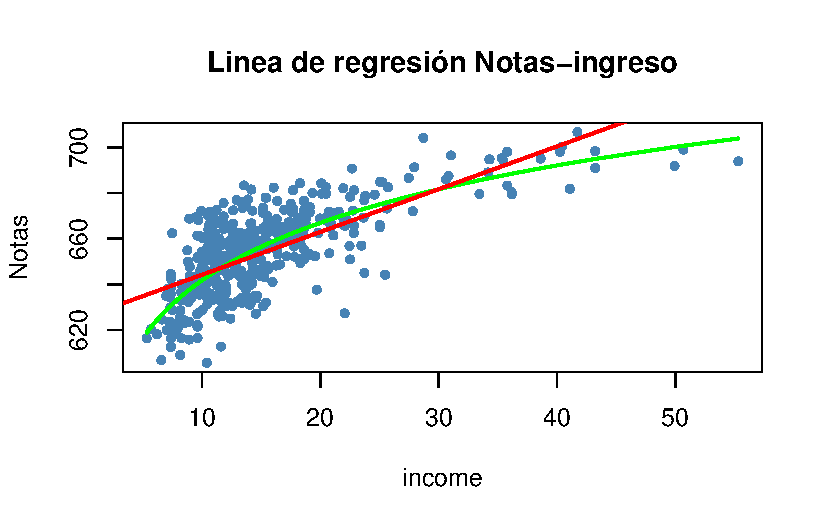
\includegraphics{cap3_files/figure-pdf/unnamed-chunk-4-1.pdf}

Volviendo a la ecuación {[}1{]}, debido a que \(exp(.)\) siempre es
positivo. {[}1{]} asegura que los valores predichos para \(y\) también
sean positivos. Aunque {[}1{]} es más complicada que un modelo lineal,
básicamente ya se sabe como interpretar los coeficientes, al obtener el
logaritmo de la ecuación {[}1{]}

\[log[E(y|x_1,...,x_k)]=\beta_0+\beta_1x_1+...+\beta_kx_k\ [2]\] es
decir, que el logaritmo del valor esperado es lineal. Por lo tanto,
mediante las propiedades de la aproximación de la función logaritmo
tenemos:

\[\%\Delta E(y|\mathbf{x})\approx(100\beta_j)\Delta x_j[3]\] Es decir,
\(100\beta_j\) es el cambio porcentual en \(E(y|\mathbf{x})\), dado un
incremento de una unidad en \(x_j\). A veces, es necesaria una
estimación más precisa y es fácil de encontrar una, al observar los
cambios discretos en el valor esperado. Manteniendo todas la variables
explicativas fijas, excepto \(x_j\) y, sea \(x_k^0\) el valor inicial y
\(x_k^1\) el valor siguiente. Entonces, el cambio proporcional en el
valor esperado es:

\[[exp(\beta_o+\mathbf{x_{k-1}\beta_{k-1}}+\beta_kx_k^1)/exp(\beta_o+\mathbf{x_{k-1}\beta_{k-1}}+\beta_kx_k^0)]-1=exp(\beta_k\Delta{x_k})-1\ [4]\]

Donde: \(\mathbf{x_{k-1}\beta_{k-1}}\) es una abreviatura de
\(\beta_1x_1+..+\beta_{k-1}x_{k-1}\) y, \(\Delta{x_k}=x_k^1-x_k^0\).
Cuando \(\Delta{x_k}=1\), la variable \(x_k\) es binaria que se cambia
de cero a uno, entonces el cambio es \(exp(\beta_k)-1\). Dada
\(\widehat{\beta}_k\), se obtiene \(exp(\widehat{\beta}_k)-1\) y se
multiplica por el 100 para transformar el cambio proporcional en un
cambio porcentual.

Si por ejemplo \(x_j=log(z_j)\) para alguna variable \(z_j>0\), entonces
su coeficiente \(\beta_j\) se interpreta como una elasticidad respecto a
\(z_j\)

Debido a que {[}1{]} es no lineal en sus parámetros, no se puede usar
métodos de regresión lineal. Entonces usamos la \textbf{estimación
máxima verosimilitud (EMV)} y también el método relacionado a la
\textbf{estimación de cuasi máxima verosimilitud (ECMV)}

A lo largo de los cursos de econometría se ha presentado la normalidad
como el supuesto de distribución estándar para regresión lineal. Este
supuesto no puede usarse en una variable de conteo (pues la distribución
normal es para variables continuas que asuman todos los valores) que
asume sólo pocos valores, la distribución será muy distinta a la normal.
En su lugar, la distribución nominal para los datos de conteo es la
\textbf{distribución Poisson}

Como nos interesa el efecto de las variables explicativas sobre \(y\),
se debe observar la distribución de Poisson condicional a
\(\mathbf{x}\). La distribución Poisson está determinada por completo
por su media, así sólo se necesita especificar \(E(y|\mathbf{x})\), esta
tiene la misma forma de {[}1{]} que se abrevia \(exp(\mathbf{x\beta})\).
Entonces, la probabilidad de que \(y\) será igual al valor \(h\),
condicional sobre \(\mathbf{x}\), es:

\[P(y=h|\mathbf{x})=exp[-exp(\mathbf{x\beta})][exp(\mathbf{x\beta})]^h/h!, h=0,1,...\ [5]\]
Donde \(h!\) denota el factorial. Esta distribución, que es la base del
\textbf{modelo de regresión de Poisson}, permite hallar las
probabilidades condicionales para cualquier valor de variables
explicativas. Por ejemplo,
\(P(y=0|\mathbf{x})=exp[-exp(\mathbf{x\beta})]\). Una vez que se tienen
las estimaciones de \(\beta_j\), se pueden insertar en las
probabilidades para diferentes valores \(\mathbf{x}\).

Dada una muestras aleatoria \([(\mathbf{x_i},y_i):i=1,2,...,n]\), se
puede construir la función \textbf{log-verosimilitud}:

\[\mathcal{L(\beta)}=\Sigma_{i=1}^n\mathcal{l_i(\beta)}=\Sigma_{i=1}^n[y_i\mathbf{x_i\beta}-exp(\mathbf{x_i\beta})]\ [6]\]
Se desecha el término \(log(y_i!)\). Esta función se maximiza usando
EMV, aunque la EMV de Poisson no es cerrada.

Igual que los modelo logit, probit y Tobit, no se pueden comparar
directamente las magnitudes de las estimaciones del Poisson de una
función exponencial con las estimaciones de MCO. se hace comparables de
la siguiente forma:

\subsubsection{Variables explicativas
continuas}\label{variables-explicativas-continuas}

Se aplica el efecto parcial de \(x_j\) respecto a
\(E(y|x_1,x_2,..,x_k)\):

\[\frac{\partial E(y|x_1,x_2,..,x_k)}{\partial x_j}=exp(\beta_0+\beta_1x_1+...+\beta_kx_k)\times \beta_j [7]\]
Es interesante el factor escalar \textbf{EPP}:

\[n^{-1}\Sigma_{i=1}^nexp(\hat{\beta}_0+\hat{\beta}_1x_1+...+\hat{\beta}_kx_k)=n^{-1}\Sigma_{i=1}^n\hat{y}_i [8]\]

es simplemente el promedio muestral \(\bar{y}\) de \(y_i\) donde se
definen los valores ajustados como
\(\widehat{y}_i=exp(\hat{\beta}_0+\mathbf{x_i\hat{\beta}})\). Es decir,
para la regresión Poisson con una función media exponencial, el promedio
de los valores ajustados es el mismo que el promedio de los resultados
originales de \(y_t\), tal como el caso de regresión lineal. Esto
simplifica el escalar de las estimaciones Poisson \(\widehat{\beta}_j\),
para hacerlas comparables a las estimaciones MCO, \(\widehat{\gamma}_j\)
para una variable explicativa continua, se puede comparar con
\(\widehat{\gamma}_j\) con \(\bar{y}.\widehat{\beta}_{j}\)

Aunque el análisis de EMV de Poisson es un primer paso para los datos de
conteo, suele ser muy restrictivo. Todas las probabilidades y los
momentos mayores de la distribución Poisson se determinan por completo
por la media. Por ejemplo, la varianza es igual a la media:

\[Var(y|\mathbf{x})=E(y|\mathbf{x})\hspace{0.5cm} [9]\] Esto es
restrictivo y se viola en muchas aplicaciones. Por fortuna, la
distribución de Poisson tiene una propiedad de robustez muy buena, es
decir, que se mantenga o no la distribución de Poisson, se obtienen
estimadores asistóticamente normales y consistentes con las \(\beta_j\)

Cuando se EMV de Poisson, pero no se supone que la distribución de
Poisson sea correcta, este análisis recibe el nombre de
\textbf{Estimación de cuasi máxima verosimilitud (ECMV)}. LA ECMV de
Poisson es muy útil debido a que esta programada en muchos paquetes
econométricos. Sin embargo, a menos que el supuesto de varianza de
Poisson {[}9{]} se mantenga, se deben ajustar los errores estándar, de
la siguiente forma:

El ajuste a los errores estándar está disponible cuando se supone que la
varianza es proporcional a la media:

\[Var(y|\mathbf{x})=\sigma^2E(y|\mathbf{x})\ [10]\] Donde: \(\sigma^2\)
es un parámetro desconocido.

\begin{itemize}
\item
  Cuando \(\sigma^2=1\) se obtiene el supuesto de varianza de Poisson
  {[}9{]}
\item
  Si \(\sigma^2>1\) la varianza es mayor que la media para toda
  \(\mathbf{x}\), esto se llama \textbf{sobredispersión} común en
  regresiones de conteo.

  \begin{itemize}
  \tightlist
  \item
    Si \(\sigma^2<1\) la varianza es menor que la media para toda
    \(\mathbf{x}\), esto se llama \textbf{subdispersión} es poco común.
  \end{itemize}
\end{itemize}

Bajo {[}10{]} es fácil ajustar los errores estándar de la EMV de
Poisson. Si \(\hat{\beta}_j\) denota la ECMV de Poisson y se definen los
residuales como \(\hat{u}_i=y_i-\hat{y}_i\), donde
\(\hat{y}_i=exp(\hat{\beta}_0+\hat{\beta}_1x_{i1}+...+\hat{\beta}_kx_{ik})\).
Un estimador consistente de
\(\sigma^2=(n-k-1)^{-1}\sum_{i=1}^n\frac{\hat{u}_i^2}{\hat{y}_i}\),
donde la división entre \(\hat{y}_i\) es el ajuste apropiado de
heterocedasticidad y \(n-k-1=gl\) dadas las \(n\) observaciones y
\(k+1\) estimadores \(\hat{\beta}_0,\hat{\beta}_1,...,\hat{\beta}_k\).
Si \(\sigma=\sqrt{\sigma^2}\), se multiplican los errores estándar
Poisson usuales por \(\hat{\sigma}\). Si \(\hat{\sigma}\) es
notablemente mayor que uno, los errores estándar corregidos pueden ser
mucho mayores que los errores estándar nominales, generalmente son
incorrectos, de la EMV de Poisson.

Bajo el supuesto de distribución de Poisson, se puede usar el
estadístico de la razón de verosimilitudes para probar las restricciones
de exclusión, que siempre, tienen la forma de \(RV=2(l_{nr}-L_r)\). Si
se tiene \(q\) restricciones de exclusión, el estadístico se distribuye
aproximadamente con \(\chi^2_q\) bajo la hipótesis nula. Bajo el
supuesto menos restrictivo de {[}10{]}, un simple ajuste está disponible
si se divide \(RV=2(l_{nr}-L_r)\) entre \(\sigma^2\) donde \(\sigma^2\)
se obtiene del modelo no restringido.

\section{Ejemplo {[}Regresión de Poisson para número de
arrestos{]}}\label{ejemplo-regresiuxf3n-de-poisson-para-nuxfamero-de-arrestos}

La base de datos \textbf{crime1} contiene información sobre arrestos
durante 1986 y otros datos, sobre 2725 hombres nacidos en California en
1960 o 1961. Cada hombre de la muestra fue arrestado al menos una vez
antes 1986.

Las variables:

\begin{itemize}
\tightlist
\item
  \textbf{narr86}: indica el número de veces que un hombre fue arrestado
  durante 1986: esta variable es cero para la mayoría de los hombres de
  la muestra (72.29\%) y varía desde 0 hasta 12. (El porcentaje de
  hombres detenidos una sola vez durante 1986 es 20.51\%)
\end{itemize}

\begin{Shaded}
\begin{Highlighting}[]
\NormalTok{pacman}\SpecialCharTok{::}\FunctionTok{p\_load}\NormalTok{(wooldridge, }
\NormalTok{               tidyverse)}

\FunctionTok{data}\NormalTok{(}\StringTok{"crime1"}\NormalTok{)}

\NormalTok{crime1 }\SpecialCharTok{\%\textgreater{}\%} 
\FunctionTok{str}\NormalTok{()}
\end{Highlighting}
\end{Shaded}

\begin{verbatim}
'data.frame':   2725 obs. of  16 variables:
 $ narr86 : int  0 2 1 2 1 0 2 5 0 0 ...
 $ nfarr86: int  0 2 1 2 1 0 2 3 0 0 ...
 $ nparr86: int  0 0 0 1 0 0 1 5 0 0 ...
 $ pcnv   : num  0.38 0.44 0.33 0.25 0 ...
 $ avgsen : num  17.6 0 22.8 0 0 ...
 $ tottime: num  35.2 0 22.8 0 0 ...
 $ ptime86: int  12 0 0 5 0 0 0 0 9 0 ...
 $ qemp86 : num  0 1 0 2 2 4 0 0 0 3 ...
 $ inc86  : num  0 0.8 0 8.8 8.1 ...
 $ durat  : num  0 0 11 0 1 ...
 $ black  : int  0 0 1 0 0 0 1 0 1 0 ...
 $ hispan : int  0 1 0 1 0 0 0 0 0 1 ...
 $ born60 : int  1 0 1 1 0 1 1 1 1 1 ...
 $ pcnvsq : num  0.1444 0.1936 0.1089 0.0625 0 ...
 $ pt86sq : int  144 0 0 25 0 0 0 0 81 0 ...
 $ inc86sq: num  0 0.64 0 77.44 65.61 ...
 - attr(*, "time.stamp")= chr "25 Jun 2011 23:03"
\end{verbatim}

\begin{Shaded}
\begin{Highlighting}[]
\CommentTok{\# Tabla de porcentaje}
\NormalTok{crime1 }\SpecialCharTok{\%\textgreater{}\%} 
  \FunctionTok{with}\NormalTok{(}\FunctionTok{table}\NormalTok{(narr86)) }\SpecialCharTok{\%\textgreater{}\%} 
  \FunctionTok{prop.table}\NormalTok{() }\SpecialCharTok{\%\textgreater{}\%} 
  \FunctionTok{round}\NormalTok{(}\AttributeTok{digits =} \DecValTok{2}\NormalTok{) }\SpecialCharTok{\%\textgreater{}\%} 
  \FunctionTok{print}\NormalTok{()}
\end{Highlighting}
\end{Shaded}

\begin{verbatim}
narr86
   0    1    2    3    4    5    6    7    9   10   12 
0.72 0.21 0.04 0.02 0.00 0.00 0.00 0.00 0.00 0.00 0.00 
\end{verbatim}

\begin{itemize}
\tightlist
\item
  \textbf{pcnv}: Es la proporción (no el porcentaje) de detenciones
  anteriores a 1986 que condujeron a una condena (?)
\end{itemize}

\begin{Shaded}
\begin{Highlighting}[]
\NormalTok{crime1 }\SpecialCharTok{\%\textgreater{}\%} 
  \FunctionTok{with}\NormalTok{(}\FunctionTok{table}\NormalTok{(pcnv)) }\SpecialCharTok{\%\textgreater{}\%} 
  \FunctionTok{round}\NormalTok{(}\AttributeTok{digits =} \DecValTok{2}\NormalTok{) }\SpecialCharTok{\%\textgreater{}\%} 
  \FunctionTok{print}\NormalTok{()}
\end{Highlighting}
\end{Shaded}

\begin{verbatim}
pcnv
                 0 0.0799999982118607 0.0900000035762787  0.100000001490116 
              1260                  2                  1                  1 
 0.109999999403954  0.129999995231628  0.140000000596046  0.170000001788139 
                 1                  3                  6                 17 
 0.180000007152557  0.200000002980232  0.219999998807907  0.230000004172325 
                 2                 24                  4                  4 
              0.25  0.259999990463257  0.270000010728836   0.28999999165535 
                53                  1                  2                 21 
 0.300000011920929  0.310000002384186  0.319999992847443  0.330000013113022 
                 4                  2                  1                139 
 0.360000014305115  0.379999995231628  0.389999985694885  0.400000005960464 
                 7                 20                  1                 40 
 0.409999996423721  0.419999986886978  0.430000007152557  0.439999997615814 
                 1                  5                 14                 10 
 0.449999988079071  0.469999998807907                0.5  0.529999971389771 
                 4                  3                313                  1 
 0.540000021457672  0.560000002384186  0.569999992847443  0.600000023841858 
                 2                  8                 11                 34 
 0.620000004768372  0.629999995231628  0.639999985694885  0.670000016689301 
                 1                  6                  2                 85 
 0.699999988079071  0.709999978542328  0.730000019073486               0.75 
                 1                  2                  1                 20 
 0.800000011920929  0.829999983310699                  1 
                 8                  3                574 
\end{verbatim}

\begin{itemize}
\tightlist
\item
  \textbf{avgsen} es la duración promedio de las condenas anteriores
  cumplidas (cero para la mayoría de casos)
\end{itemize}

\begin{Shaded}
\begin{Highlighting}[]
\NormalTok{crime1 }\SpecialCharTok{\%\textgreater{}\%} 
  \FunctionTok{with}\NormalTok{(}\FunctionTok{table}\NormalTok{(avgsen)) }\SpecialCharTok{\%\textgreater{}\%} 
  \FunctionTok{print}\NormalTok{()}
\end{Highlighting}
\end{Shaded}

\begin{verbatim}
avgsen
                0 0.300000011920929 0.800000011920929 0.899999976158142 
             2591                 1                 2                 2 
 1.10000002384186  1.39999997615814  2.20000004768372  2.29999995231628 
                5                 1                 1                 1 
 2.59999990463257  2.90000009536743               3.5                 4 
                2                 1                 1                 2 
 4.30000019073486  4.80000019073486  4.90000009536743               5.5 
                1                 1                 1                 2 
 5.59999990463257                 6  6.09999990463257  6.19999980926514 
                4                 1                 2                 1 
 6.30000019073486  6.69999980926514  6.90000009536743  7.09999990463257 
                1                 1                 1                 3 
 7.19999980926514  7.59999990463257  7.80000019073486  7.90000009536743 
                1                 1                 2                 1 
 8.10000038146973  8.19999980926514  8.30000019073486  8.39999961853027 
                1                 1                 1                 1 
 8.60000038146973  8.89999961853027                 9  9.10000038146973 
                2                 1                 2                 1 
 9.30000019073486               9.5  9.60000038146973  9.69999980926514 
                1                 1                 1                 2 
 9.80000019073486  9.89999961853027                10              10.5 
                1                 1                 1                 1 
 10.6000003814697  10.6999998092651  10.8999996185303                11 
                1                 1                 2                 1 
 11.1000003814697  11.3000001907349  11.3999996185303  11.6000003814697 
                1                 1                 1                 2 
 11.6999998092651  11.8000001907349  11.8999996185303  12.1000003814697 
                1                 2                 3                 1 
 12.1999998092651  12.3999996185303              12.5  12.6999998092651 
                2                 1                 2                 1 
 12.8999996185303  13.3000001907349  13.3999996185303  13.6999998092651 
                1                 1                 1                 1 
 14.1999998092651  14.3000001907349  14.3999996185303  14.8000001907349 
                1                 1                 1                 1 
               15  15.6999998092651                16  16.1000003814697 
                1                 1                 1                 1 
 16.2000007629395              16.5  16.6000003814697                17 
                1                 1                 1                 1 
 17.1000003814697  17.6000003814697  17.7000007629395  18.3999996185303 
                1                 1                 1                 3 
             18.5  18.7000007629395  18.8999996185303  19.2999992370605 
                1                 1                 2                 2 
 20.2999992370605  20.6000003814697  21.7000007629395  21.7999992370605 
                1                 1                 1                 1 
               22  22.7999992370605              23.5  23.8999996185303 
                1                 1                 1                 1 
 24.3999996185303  24.6000003814697  30.3999996185303  31.2999992370605 
                1                 2                 1                 1 
 31.7000007629395  31.8999996185303  35.4000015258789  36.0999984741211 
                1                 1                 1                 1 
               39              40.5  47.0999984741211  59.2000007629395 
                1                 1                 1                 1 
\end{verbatim}

\begin{itemize}
\tightlist
\item
  \textbf{tottime}: tiempo en prisión desde los 18 años (meses)
\end{itemize}

\begin{Shaded}
\begin{Highlighting}[]
\NormalTok{crime1 }\SpecialCharTok{\%\textgreater{}\%} 
  \FunctionTok{with}\NormalTok{(}\FunctionTok{table}\NormalTok{(tottime)) }\SpecialCharTok{\%\textgreater{}\%} 
  \FunctionTok{print}\NormalTok{()}
\end{Highlighting}
\end{Shaded}

\begin{verbatim}
tottime
                0 0.300000011920929 0.800000011920929 0.899999976158142 
             2591                 1                 2                 2 
 1.10000002384186  1.39999997615814  2.20000004768372  2.29999995231628 
                5                 1                 1                 1 
 2.59999990463257  2.90000009536743                 4  4.80000019073486 
                2                 1                 2                 1 
              5.5  5.59999990463257                 6  6.19999980926514 
                1                 2                 1                 1 
 6.69999980926514                 7  7.09999990463257  7.19999980926514 
                1                 1                 1                 1 
 7.59999990463257  7.80000019073486  8.10000038146973  8.19999980926514 
                1                 1                 1                 1 
 8.30000019073486  8.60000038146973  8.89999961853027                 9 
                1                 2                 1                 1 
 9.10000038146973  9.30000019073486               9.5  9.60000038146973 
                1                 1                 1                 1 
 9.80000019073486  9.89999961853027              10.5  10.8999996185303 
                1                 1                 1                 1 
               11  11.1000003814697  11.1999998092651  11.3000001907349 
                2                 1                 1                 1 
 11.3999996185303  11.6000003814697  11.6999998092651  11.8000001907349 
                1                 1                 1                 1 
 11.8999996185303  12.1999998092651  12.3999996185303              12.5 
                3                 4                 1                 2 
 12.8999996185303  13.3000001907349  13.3999996185303  13.6999998092651 
                1                 1                 1                 1 
 14.1999998092651  14.3000001907349  14.3999996185303  14.6999998092651 
                2                 1                 1                 1 
 15.6999998092651  16.1000003814697              16.5  16.6000003814697 
                1                 1                 1                 1 
 16.7999992370605                17  17.1000003814697                18 
                1                 1                 1                 1 
 18.3999996185303              18.5  18.8999996185303  19.2999992370605 
                2                 1                 2                 2 
 19.3999996185303                20  20.2999992370605  20.7000007629395 
                1                 1                 1                 1 
 21.2000007629395  21.2999992370605  21.3999996185303  21.7000007629395 
                1                 1                 1                 1 
 21.7999992370605                22  22.3999996185303  22.7999992370605 
                1                 1                 1                 1 
 23.2000007629395              23.5  23.7000007629395  23.8999996185303 
                1                 1                 1                 1 
 24.2000007629395  24.3999996185303  24.6000003814697  25.2000007629395 
                1                 1                 1                 1 
 25.7999992370605  29.1000003814697  29.6000003814697                30 
                1                 1                 1                 1 
 30.3999996185303  31.2000007629395  31.2999992370605  31.8999996185303 
                1                 1                 1                 1 
               32  32.4000015258789  35.2000007629395  35.4000015258789 
                1                 1                 1                 3 
 36.0999984741211  36.7999992370605  37.4000015258789  38.0999984741211 
                1                 1                 1                 1 
               39              40.5  41.2000007629395  43.5999984741211 
                1                 1                 1                 1 
 47.0999984741211  49.2000007629395  59.2000007629395  63.4000015258789 
                1                 1                 1                 1 
\end{verbatim}

\begin{itemize}
\tightlist
\item
  \textbf{ptime86}: es el tiempo en meses que se ha pasado en prisión
  durante 1986
\end{itemize}

\begin{Shaded}
\begin{Highlighting}[]
\NormalTok{crime1 }\SpecialCharTok{\%\textgreater{}\%} 
  \FunctionTok{with}\NormalTok{(}\FunctionTok{table}\NormalTok{(ptime86)) }\SpecialCharTok{\%\textgreater{}\%} 
  \FunctionTok{print}\NormalTok{()}
\end{Highlighting}
\end{Shaded}

\begin{verbatim}
ptime86
   0    1    2    3    4    5    6    7    8    9   10   11   12 
2594    7   15    8    7    5   10    7    2    4    4    4   58 
\end{verbatim}

\begin{itemize}
\tightlist
\item
  \textbf{qemp86}: es la cantidad de trimestres que la persona tuvo
  empleo en 1986 (de cero a cuatro)
\end{itemize}

\begin{Shaded}
\begin{Highlighting}[]
\NormalTok{crime1 }\SpecialCharTok{\%\textgreater{}\%} 
  \FunctionTok{with}\NormalTok{(}\FunctionTok{table}\NormalTok{(qemp86)) }\SpecialCharTok{\%\textgreater{}\%} 
  \FunctionTok{print}\NormalTok{()}
\end{Highlighting}
\end{Shaded}

\begin{verbatim}
qemp86
                0 0.600000023841858 0.899999976158142                 1 
              648                 1                 1               294 
 1.39999997615814  1.60000002384186  1.70000004768372  1.79999995231628 
                1                 1                 1                 3 
                2  2.09999990463257                 3  3.40000009536743 
              337                 1               437                 1 
                4 
              999 
\end{verbatim}

\begin{itemize}
\item
  \textbf{ince86}: ingresos legales, 1986, \$100s
\item
  \textbf{black} 1 si es negro, cero otro caso
\item
  \textbf{hispan} 1 si es hispano, cero otro caso
\item
  \textbf{born60} 1 nacido en 1960, cero otro caso
\end{itemize}

\subsubsection{Modelo de regresión
Poisson}\label{modelo-de-regresiuxf3n-poisson}

\[
\begin{aligned}
E[narr86|\mathbf{x}]=exp\left(\beta_0+\beta_1pcnv+\beta_2avgsen+\beta_3tottime\\
+\beta_4ptime86+\beta_5qemp86+\beta_6ince86+\\
+\delta_1black+\delta_2hispan+\delta_3born\right)
\end{aligned}
\]

\begin{Shaded}
\begin{Highlighting}[]
\CommentTok{\# Comprobar la variable de conteo}

\NormalTok{crime1 }\SpecialCharTok{\%\textgreater{}\%} 
  \FunctionTok{with}\NormalTok{(}\FunctionTok{table}\NormalTok{(narr86)) }\SpecialCharTok{\%\textgreater{}\%} 
  \FunctionTok{print}\NormalTok{()}
\end{Highlighting}
\end{Shaded}

\begin{verbatim}
narr86
   0    1    2    3    4    5    6    7    9   10   12 
1970  559  121   42   12   13    4    1    1    1    1 
\end{verbatim}

\begin{Shaded}
\begin{Highlighting}[]
\CommentTok{\# Graficar la variable}
\FunctionTok{ggplot}\NormalTok{(crime1, }\FunctionTok{aes}\NormalTok{(}\AttributeTok{x =}\NormalTok{ narr86)) }\SpecialCharTok{+} 
  \FunctionTok{geom\_histogram}\NormalTok{(}\AttributeTok{binwidth =} \FloatTok{0.5}\NormalTok{, }
                 \AttributeTok{color =} \StringTok{"black"}\NormalTok{, }
                 \AttributeTok{fill =} \StringTok{"skyblue"}\NormalTok{,}
                 \AttributeTok{alpha =} \FloatTok{0.5}\NormalTok{) }\SpecialCharTok{+} 
  \FunctionTok{geom\_density}\NormalTok{(}\AttributeTok{alpha =} \FloatTok{0.5}\NormalTok{, }
               \AttributeTok{color =} \StringTok{"red"}\NormalTok{) }\SpecialCharTok{+} 
  \FunctionTok{labs}\NormalTok{(}\AttributeTok{title =} \StringTok{"Histograma con densidad de kernel del número de arrestos"}\NormalTok{, }
       \AttributeTok{x =} \StringTok{"Valor"}\NormalTok{, }\AttributeTok{y =} \StringTok{"Frecuencia"}\NormalTok{) }\SpecialCharTok{+} 
  \FunctionTok{theme\_classic}\NormalTok{()}
\end{Highlighting}
\end{Shaded}

\includegraphics{cap3_files/figure-pdf/ajuste-1.pdf}

Ajustar el modelo usando MCO

\begin{Shaded}
\begin{Highlighting}[]
\NormalTok{narr86.MCO }\OtherTok{\textless{}{-}} \FunctionTok{lm}\NormalTok{(narr86}\SpecialCharTok{\textasciitilde{}}
\NormalTok{                   pcnv}\SpecialCharTok{+}
\NormalTok{                   avgsen}\SpecialCharTok{+}
\NormalTok{                   tottime}\SpecialCharTok{+}
\NormalTok{                   ptime86}\SpecialCharTok{+}
\NormalTok{                   qemp86}\SpecialCharTok{+}
\NormalTok{                   inc86}\SpecialCharTok{+}
\NormalTok{                   black}\SpecialCharTok{+}
\NormalTok{                   hispan}\SpecialCharTok{+}
                   \FunctionTok{I}\NormalTok{(hispan}\SpecialCharTok{*}\NormalTok{black)}\SpecialCharTok{+}
\NormalTok{                   born60,}
\NormalTok{                 crime1)}

\NormalTok{narr86.MCO2 }\OtherTok{\textless{}{-}} \FunctionTok{lm}\NormalTok{(narr86}\SpecialCharTok{\textasciitilde{}}
\NormalTok{                   hispan,}
\NormalTok{                 crime1)}

\FunctionTok{library}\NormalTok{(stargazer)}
\FunctionTok{stargazer}\NormalTok{(narr86.MCO, narr86.MCO2,}\AttributeTok{type =} \StringTok{"text"}\NormalTok{)}
\end{Highlighting}
\end{Shaded}

\begin{verbatim}

====================================================================
                                  Dependent variable:               
                    ------------------------------------------------
                                         narr86                     
                              (1)                      (2)          
--------------------------------------------------------------------
pcnv                       -0.132***                                
                            (0.040)                                 
                                                                    
avgsen                       -0.011                                 
                            (0.012)                                 
                                                                    
tottime                      0.012                                  
                            (0.009)                                 
                                                                    
ptime86                    -0.041***                                
                            (0.009)                                 
                                                                    
qemp86                     -0.051***                                
                            (0.014)                                 
                                                                    
inc86                      -0.001***                                
                            (0.0003)                                
                                                                    
black                       0.327***                                
                            (0.045)                                 
                                                                    
hispan                      0.194***                0.110***        
                            (0.040)                  (0.040)        
                                                                    
I(hispan * black)                                                   
                                                                    
                                                                    
born60                       -0.022                                 
                            (0.033)                                 
                                                                    
Constant                    0.577***                0.380***        
                            (0.038)                  (0.019)        
                                                                    
--------------------------------------------------------------------
Observations                 2,725                    2,725         
R2                           0.072                    0.003         
Adjusted R2                  0.069                    0.002         
Residual Std. Error    0.829 (df = 2715)        0.858 (df = 2723)   
F Statistic         23.572*** (df = 9; 2715) 7.671*** (df = 1; 2723)
====================================================================
Note:                                    *p<0.1; **p<0.05; ***p<0.01
\end{verbatim}

El modelo MCO supone que la variable \(y\) es cuantitativa
aproximadamente continua, tenemos una variable de conteo

\begin{Shaded}
\begin{Highlighting}[]
\FunctionTok{summary}\NormalTok{(narr86.MCO}\SpecialCharTok{$}\NormalTok{fitted.values)}
\end{Highlighting}
\end{Shaded}

\begin{verbatim}
   Min. 1st Qu.  Median    Mean 3rd Qu.    Max. 
-0.4978  0.2346  0.4092  0.4044  0.5541  1.0210 
\end{verbatim}

No esta ajustando bien, pues arroja valores ajustados negativos el
modelo MCO, recordar que la variable \(y\) es de conteo y comienza en
cero y termina en 12

\textbf{Ajuste con el modelo Poisson}

\begin{Shaded}
\begin{Highlighting}[]
\NormalTok{narr86.poisson }\OtherTok{\textless{}{-}} \FunctionTok{glm}\NormalTok{(narr86}\SpecialCharTok{\textasciitilde{}}
\NormalTok{                   pcnv}\SpecialCharTok{+}
\NormalTok{                   avgsen}\SpecialCharTok{+}
\NormalTok{                   tottime}\SpecialCharTok{+}
\NormalTok{                   ptime86}\SpecialCharTok{+}
\NormalTok{                   qemp86}\SpecialCharTok{+}
\NormalTok{                   inc86}\SpecialCharTok{+}
\NormalTok{                   black}\SpecialCharTok{+}
\NormalTok{                   hispan}\SpecialCharTok{+}
\NormalTok{                   born60,}
\NormalTok{                 crime1,}
                 \AttributeTok{family =} \FunctionTok{poisson}\NormalTok{(}\AttributeTok{link =} \StringTok{"log"}\NormalTok{))}

\CommentTok{\# Comparo el modelo Possion y MCO}

\FunctionTok{stargazer}\NormalTok{(narr86.MCO, narr86.poisson, }
          \AttributeTok{type =} \StringTok{"text"}\NormalTok{,}
          \AttributeTok{df=}\NormalTok{F,}
          \AttributeTok{digits =} \DecValTok{3}\NormalTok{,}
          \AttributeTok{title =} \StringTok{"Tabla 1. Determinantes del número de arrestos de hombres jóvenes"}\NormalTok{,}
          \AttributeTok{dep.var.caption =} \StringTok{"Variable dependiente: Número de arrestos"}\NormalTok{,}
          \AttributeTok{header =}\NormalTok{ F,}
          \AttributeTok{column.labels =} \FunctionTok{c}\NormalTok{(}\StringTok{"MCO"}\NormalTok{, }\StringTok{"Poisson"}\NormalTok{),}
          \AttributeTok{model.names =}\NormalTok{ F,}
          \AttributeTok{report =} \StringTok{"vct*"}\NormalTok{)}
\end{Highlighting}
\end{Shaded}

\begin{verbatim}

Tabla 1. Determinantes del número de arrestos de hombres jóvenes
=============================================================
                    Variable dependiente: Número de arrestos 
                    -----------------------------------------
                                     narr86                  
                            MCO                Poisson       
                            (1)                  (2)         
-------------------------------------------------------------
pcnv                       -0.132               -0.402       
                       t = -3.264***        t = -4.726***    
                                                             
avgsen                     -0.011               -0.024       
                         t = -0.926           t = -1.192     
                                                             
tottime                    0.012                0.024        
                         t = 1.279            t = 1.660*     
                                                             
ptime86                    -0.041               -0.099       
                       t = -4.638***        t = -4.763***    
                                                             
qemp86                     -0.051               -0.038       
                       t = -3.542***          t = -1.310     
                                                             
inc86                      -0.001               -0.008       
                       t = -4.261***        t = -7.762***    
                                                             
black                      0.327                0.661        
                        t = 7.199***         t = 8.950***    
                                                             
hispan                     0.194                0.500        
                        t = 4.880***         t = 6.761***    
                                                             
I(hispan * black)                                            
                                                             
                                                             
born60                     -0.022               -0.051       
                         t = -0.675           t = -0.797     
                                                             
Constant                   0.577                -0.600       
                       t = 15.215***        t = -8.916***    
                                                             
-------------------------------------------------------------
Observations               2,725                2,725        
R2                         0.072                             
Adjusted R2                0.069                             
Log Likelihood                                -2,248.761     
Akaike Inf. Crit.                             4,517.522      
Residual Std. Error        0.829                             
F Statistic              23.572***                           
=============================================================
Note:                             *p<0.1; **p<0.05; ***p<0.01
\end{verbatim}

\begin{Shaded}
\begin{Highlighting}[]
\FunctionTok{mean}\NormalTok{(crime1}\SpecialCharTok{$}\NormalTok{narr86)}
\end{Highlighting}
\end{Shaded}

\begin{verbatim}
[1] 0.4044037
\end{verbatim}

Es común en los modelos \textbf{Poisson} que exista un mal cálculo de
los errores estándar, pues puede haber sobre o sub dispersión de la
varianza de acuerdo a la ecuación {[}10{]}

\subsection{\texorpdfstring{Estimación de
\(\sigma^2\)}{Estimación de \textbackslash sigma\^{}2}}\label{estimaciuxf3n-de-sigma2}

Recordemos la ecuación:

\[\sigma^2=(n-k-1)^{-1}\Sigma_{i=1}^n\frac{\widehat{u}_i^2}{\widehat{y}_i} [11]\]
También recordar la ecuación para los residuales

\[\widehat{u}_i=y_i-\widehat{y}_i [12]\]

\begin{Shaded}
\begin{Highlighting}[]
\NormalTok{residuales }\OtherTok{\textless{}{-}}\NormalTok{ narr86.poisson}\SpecialCharTok{$}\NormalTok{y}\SpecialCharTok{{-}}\NormalTok{ narr86.poisson}\SpecialCharTok{$}\NormalTok{fitted.values}

\NormalTok{sigma2}\OtherTok{\textless{}{-}}\NormalTok{(}\FunctionTok{sum}\NormalTok{(residuales}\SpecialCharTok{\^{}}\DecValTok{2}\SpecialCharTok{/}\NormalTok{narr86.poisson}\SpecialCharTok{$}\NormalTok{fitted.values))}\SpecialCharTok{/}\NormalTok{narr86.MCO[[}\StringTok{"df.residual"}\NormalTok{]]}
\NormalTok{sigma2}
\end{Highlighting}
\end{Shaded}

\begin{verbatim}
[1] 1.516788
\end{verbatim}

\begin{Shaded}
\begin{Highlighting}[]
\NormalTok{raiz.sigma }\OtherTok{\textless{}{-}} \FunctionTok{sqrt}\NormalTok{(sigma2)}
\NormalTok{raiz.sigma}
\end{Highlighting}
\end{Shaded}

\begin{verbatim}
[1] 1.23158
\end{verbatim}

Comprobamos que en este caso \(\widehat{\sigma}^2\approx1.52>1\),
entonces existe \textbf{sobredispersión} por lo que no se cumple la
{[}9{]} \(Var(y|\mathbf{X})=E(y|\mathbf{X})\). Por lo tanto, se esta
analizando con la \textbf{ECMV}

\subsection{Ajustar los errores
estándar}\label{ajustar-los-errores-estuxe1ndar}

\begin{Shaded}
\begin{Highlighting}[]
\FunctionTok{library}\NormalTok{(sandwich)}
\NormalTok{ees.ajustados}\OtherTok{\textless{}{-}}\FunctionTok{list}\NormalTok{(}\FunctionTok{sqrt}\NormalTok{(}\FunctionTok{diag}\NormalTok{(}\FunctionTok{vcovHC}\NormalTok{(narr86.MCO, }\AttributeTok{type =} \StringTok{"HC1"}\NormalTok{))),}
\NormalTok{                    raiz.sigma}\SpecialCharTok{*}\FunctionTok{sqrt}\NormalTok{(}\FunctionTok{diag}\NormalTok{(}\FunctionTok{vcovHC}\NormalTok{(narr86.poisson, }\AttributeTok{type =} \StringTok{"HC1"}\NormalTok{))))}

\FunctionTok{stargazer}\NormalTok{(narr86.MCO, narr86.poisson, }
          \AttributeTok{type =} \StringTok{"text"}\NormalTok{,}
          \AttributeTok{df=}\NormalTok{F,}
          \AttributeTok{digits =} \DecValTok{3}\NormalTok{,}
          \AttributeTok{title =} \StringTok{"Tabla 2. Determinantes del número de arrestos de hombres jóvenes (ESHRA)"}\NormalTok{,}
          \AttributeTok{dep.var.caption =} \StringTok{"Variable dependiente: Número de arrestos"}\NormalTok{,}
          \AttributeTok{header =}\NormalTok{ F,}
          \AttributeTok{column.labels =} \FunctionTok{c}\NormalTok{(}\StringTok{"Lineal MCO"}\NormalTok{, }\StringTok{"Exponecial ECMV{-}Poisson"}\NormalTok{),}
          \AttributeTok{model.names =}\NormalTok{ F,}
          \AttributeTok{se=}\NormalTok{ees.ajustados)}
\end{Highlighting}
\end{Shaded}

\begin{verbatim}

Tabla 2. Determinantes del número de arrestos de hombres jóvenes (ESHRA)
=============================================================
                    Variable dependiente: Número de arrestos 
                    -----------------------------------------
                                     narr86                  
                       Lineal MCO     Exponecial ECMV-Poisson
                           (1)                  (2)          
-------------------------------------------------------------
pcnv                    -0.132***            -0.402***       
                         (0.034)              (0.125)        
                                                             
avgsen                   -0.011               -0.024         
                         (0.014)              (0.029)        
                                                             
tottime                   0.012                0.024         
                         (0.013)              (0.025)        
                                                             
ptime86                 -0.041***            -0.099***       
                         (0.007)              (0.028)        
                                                             
qemp86                  -0.051***             -0.038         
                         (0.014)              (0.042)        
                                                             
inc86                   -0.001***            -0.008***       
                        (0.0002)              (0.002)        
                                                             
black                   0.327***             0.661***        
                         (0.058)              (0.123)        
                                                             
hispan                  0.194***             0.500***        
                         (0.040)              (0.114)        
                                                             
I(hispan * black)                                            
                                                             
                                                             
born60                   -0.022               -0.051         
                         (0.032)              (0.100)        
                                                             
Constant                0.577***             -0.600***       
                         (0.043)              (0.110)        
                                                             
-------------------------------------------------------------
Observations              2,725                2,725         
R2                        0.072                              
Adjusted R2               0.069                              
Log Likelihood                              -2,248.761       
Akaike Inf. Crit.                            4,517.522       
Residual Std. Error       0.829                              
F Statistic             23.572***                            
=============================================================
Note:                             *p<0.1; **p<0.05; ***p<0.01
\end{verbatim}

\subsection{Interpretación}\label{interpretaciuxf3n}

Como se puede ver en la Tabla 2 los errores estándar MCO y Poisson son
heterocedasticos-robustos. Los errores estándar de Poisson han sido
multiplicados por el valor de sigma \(\widehat\sigma=1.232\), lo cual
incide sobre la prueba \(t\) y por ende en su significancia estadística.

Los coeficientes del MCO y Poisson no son comparables directamente y
tienen significados muy diferentes. Por ejemplo, el coeficiente de
\emph{pcnv} implica que, si \(\vartriangle{pcnv}=0.10\) el número
esperado de arrestos deciende en 0.013 (\(0.10\times0.132\approx0.013\))
(\emph{pcnv} es la proporcion de arrestos previos que desembocaron en
una condena). El coeficiente de Poisson implica que
\(\Delta{pcnv}=0.10\) reduce los arresto en cerca de 4\%
\([0.402\times0.10\approx 0.0402]\) y se multiplica esto por el 100\%
para obtener el efecto porcentual. Como cuestión de políticas, esto
siguiere que se pueden reducir los arrestos generales en 4\% si se
incremente la probabilidad de condena en 0.10.

El coeficiente de Poisson de \textbf{black} implica que, \emph{ceteris
paribus}, el número esperado de arrestos para los hombres negros se
estima cerca de \(100\times[exp(0.661)-1]\approx93.7\), es decir que la
probabilidad de arrestos para los hombres negros es 93.7\% mayor que
para los hombres blancos con los mismos valores de las variables
explicativas.

\begin{Shaded}
\begin{Highlighting}[]
\NormalTok{hispan}\OtherTok{\textless{}{-}}\NormalTok{(}\FunctionTok{exp}\NormalTok{(}\FunctionTok{coef}\NormalTok{(narr86.poisson)[}\DecValTok{9}\NormalTok{])}\SpecialCharTok{{-}}\DecValTok{1}\NormalTok{)}\SpecialCharTok{*}\DecValTok{100}
\NormalTok{hispan}
\end{Highlighting}
\end{Shaded}

\begin{verbatim}
  hispan 
64.84134 
\end{verbatim}

El coeficiente de Poisson de \textbf{hispan} implica que, \emph{ceteris
paribus}, el número esperado de arrestos para los hombres hispanos se
estima cerca de \(100\times[exp(0.5)-1]\approx 64.84\), es decir que la
probabilidad de arrestos para los hombres hispanos es 64.87\% mayor que
para los hombres no hispanos con los mismos valores de las variables
explicativas.

\subsection{Efectos marginales de la Regresión Exponencial
EMCV-Poisson}\label{efectos-marginales-de-la-regresiuxf3n-exponencial-emcv-poisson}

\begin{Shaded}
\begin{Highlighting}[]
\FunctionTok{library}\NormalTok{(mfx)}
\FunctionTok{poissonmfx}\NormalTok{(narr86}\SpecialCharTok{\textasciitilde{}}
\NormalTok{                  pcnv}\SpecialCharTok{+}
\NormalTok{                  avgsen}\SpecialCharTok{+}
\NormalTok{                  tottime}\SpecialCharTok{+}
\NormalTok{                  ptime86}\SpecialCharTok{+}
\NormalTok{                  qemp86}\SpecialCharTok{+}
\NormalTok{                  inc86}\SpecialCharTok{+}
\NormalTok{                  black}\SpecialCharTok{+}
\NormalTok{                  hispan}\SpecialCharTok{+}
\NormalTok{                  born60,}
\NormalTok{               crime1)}
\end{Highlighting}
\end{Shaded}

\begin{verbatim}
Call:
poissonmfx(formula = narr86 ~ pcnv + avgsen + tottime + ptime86 + 
    qemp86 + inc86 + black + hispan + born60, data = crime1)

Marginal Effects:
              dF/dx   Std. Err.       z     P>|z|    
pcnv    -0.13218998  0.02770671 -4.7710 1.833e-06 ***
avgsen  -0.00782541  0.00656405 -1.1922   0.23320    
tottime  0.00806178  0.00485401  1.6608   0.09674 .  
ptime86 -0.03244365  0.00677624 -4.7879 1.686e-06 ***
qemp86  -0.01251507  0.00960118 -1.3035   0.19241    
inc86   -0.00266002  0.00031733 -8.3825 < 2.2e-16 ***
black    0.27712004  0.03843968  7.2092 5.627e-13 ***
hispan   0.19144813  0.03242309  5.9047 3.533e-09 ***
born60  -0.01668211  0.02079586 -0.8022   0.42245    
---
Signif. codes:  0 '***' 0.001 '**' 0.01 '*' 0.05 '.' 0.1 ' ' 1

dF/dx is for discrete change for the following variables:

[1] "black"  "hispan" "born60"
\end{verbatim}

\subsection{Interpretaciones:}\label{interpretaciones-2}

\begin{itemize}
\tightlist
\item
  Como se puede observar los efectos marginales de Poisson ya son
  comparables a los coeficientes de MCO, de tal manera que, el
  \textbf{EPP} de Poisson para la variables \textbf{pcnv} es igual al
  coeficiente de MCO, es decir ambos son de \textbf{-0.13}
  aproximadamente. Donde existe diferencias marcadas entre el
  \textbf{EPP} y coeficiente de MCO es en \textbf{black} y en
  \textbf{hispan}. De la misma manera que se hizo en las
  interpretaciones de la Tabla 2 se debe aproximar mejor el efecto
  parcial de las variables binarias usando la ecuación {[}4{]}. Por
  ejemplo para \textbf{black}:
\end{itemize}

\begin{Shaded}
\begin{Highlighting}[]
\NormalTok{black.epp }\OtherTok{\textless{}{-}}\DecValTok{100}\SpecialCharTok{*}\NormalTok{(}\FunctionTok{exp}\NormalTok{(}\FloatTok{0.27712004}\NormalTok{)}\SpecialCharTok{{-}}\DecValTok{1}\NormalTok{)}
\NormalTok{black.epp}
\end{Highlighting}
\end{Shaded}

\begin{verbatim}
[1] 31.93247
\end{verbatim}

El coeficiente de Poisson de \textbf{black} de los efectos marginales
implica que, \emph{ceteris paribus}, el número esperado de arrestos para
los hombres negros se estima cerca de
\(100\times[exp(0.2771)-1]\approx31.93\), es decir que el porcentaje de
arrestos para los hombres negros es 31.93\% mayor que para los hombres
blancos con los mismos valores de las variables explicativas.

\begin{Shaded}
\begin{Highlighting}[]
\NormalTok{hispan.epp }\OtherTok{\textless{}{-}}\DecValTok{100}\SpecialCharTok{*}\NormalTok{(}\FunctionTok{exp}\NormalTok{(}\FloatTok{0.19144813}\NormalTok{)}\SpecialCharTok{{-}}\DecValTok{1}\NormalTok{)}
\NormalTok{hispan.epp}
\end{Highlighting}
\end{Shaded}

\begin{verbatim}
[1] 21.1002
\end{verbatim}

\bookmarksetup{startatroot}

\chapter{Modelo de Dos Partes}\label{modelo-de-dos-partes}

\section{Motivación}\label{motivaciuxf3n-1}

¿Qué sucede si se concluye que el modelo Tobit es inadecuado? Existen
modelos que suelen conocerse como modelos de \textbf{dos partes} o de
\textbf{obstáculos}, que se pueden usar cuando Tobit es inadecuado.

\section{Descripción general}\label{descripciuxf3n-general}

Los modelos de dos partes o de obstáculos se usan para modelar variables
estrictamente positivas con una gran cantidad de valores cero
\(y\geq0\). En consecuencia, existe una suerte de mezcla de una
distribución binomial \(y=1;y=0\) y una distribución estrictamente
positiva \(y>0\). En este caso, nos centramos en una distribución
aproximadamente continua para valores positivos, aunque, este modelo se
puede usar también para datos de conteo. El código en R se puede
encontrar
\href{https://raw.githubusercontent.com/dincerti/dincerti.github.io/master/_rmd-posts/twopart.R}{aquí}

\section{Ejemplo de aplicación}\label{ejemplo-de-aplicaciuxf3n}

Recordemos el modelo

\[
\widehat{hours}=\Phi\left(\frac{\beta_0+\mathbf{X\beta}}{\sigma}\right)
\] Donde las variables explicativas son:

\begin{itemize}
\item
  \(nwifeinc\): Salario de esposo en miles de dólares
\item
  \(educ\): años de educación
\item
  \(exper:\) años de experiencia
\item
  \(exper^2\): años de experiencia al cuadrado
\item
  \(age:\) edad de las mujeres
\item
  \(kidslt6\): Niños menores a seis años
\item
  \(kidsge6\): Niños entres 6 y 18 años
\end{itemize}

\begin{Shaded}
\begin{Highlighting}[]
\NormalTok{pacman}\SpecialCharTok{::}\FunctionTok{p\_load}\NormalTok{(wooldridge, }
\NormalTok{               tidyverse, }
\NormalTok{               twopartm, }
\NormalTok{               stargazer, }
\NormalTok{               data.table)}
\FunctionTok{data}\NormalTok{(}\StringTok{"mroz"}\NormalTok{)}
\CommentTok{\#mirar la distribución de la variable hours}

\FunctionTok{hist}\NormalTok{(mroz}\SpecialCharTok{$}\NormalTok{hours, }
     \AttributeTok{probability =}\NormalTok{ T,}
     \AttributeTok{main =} \StringTok{"Histograma de hours con curva normal"}\NormalTok{,}
     \AttributeTok{ylab=}\StringTok{"Densidad"}\NormalTok{)}

\FunctionTok{lines}\NormalTok{(}\FunctionTok{density}\NormalTok{(mroz}\SpecialCharTok{$}\NormalTok{hours), }
      \AttributeTok{col=}\StringTok{"blue"}\NormalTok{,}
      \AttributeTok{lwd=}\DecValTok{2}\NormalTok{)}
\end{Highlighting}
\end{Shaded}

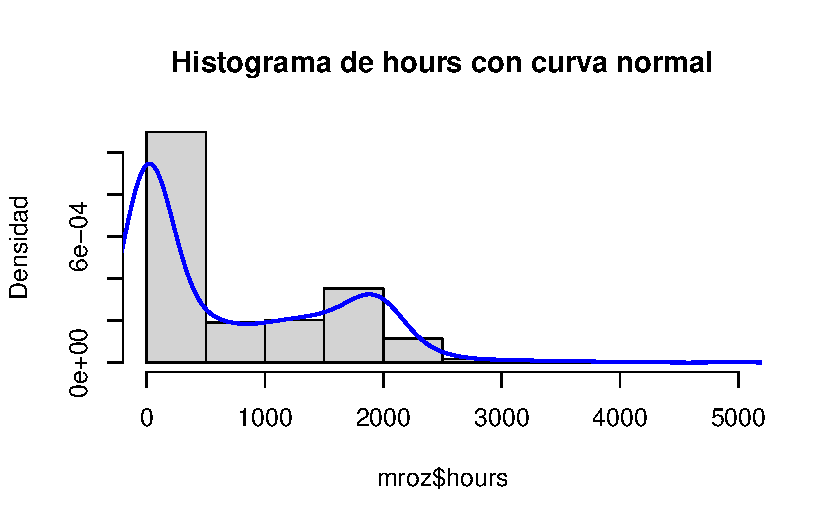
\includegraphics{cap4_files/figure-pdf/mroz-1.pdf}

La distribución de las horas esta muy sesgada a la derecha, hay muchos
valores de cero y muy pocos grandes. Esto siguiere que un modelo de dos
partes podría ser apropiado para estos datos. Las horas trabajadas no
siguen una distribución normal. Las distribuciones sesgadas a la derecha
comunes que se podrían usar para modelar las horas trabajadas son: la
distribución \textbf{lognormal} y la distribución \textbf{gamma}.

Si los datos siguen una distribución logarítmica normal, entonces el
registro de horas trabajadas sigue una distribución normal

\begin{Shaded}
\begin{Highlighting}[]
\CommentTok{\# Transformación de la variable hours a log(hours)}

\NormalTok{mroz}\SpecialCharTok{$}\NormalTok{loghours }\OtherTok{\textless{}{-}} \FunctionTok{ifelse}\NormalTok{(mroz}\SpecialCharTok{$}\NormalTok{hours}\SpecialCharTok{\textgreater{}}\DecValTok{0}\NormalTok{, }\FunctionTok{log}\NormalTok{(mroz}\SpecialCharTok{$}\NormalTok{hours), }\ConstantTok{NA}\NormalTok{)}

\CommentTok{\# Miremos la distribución de loghours 428}

\NormalTok{histDenNorm1 }\OtherTok{\textless{}{-}} \ControlFlowTok{function}\NormalTok{ (x, ...) \{}
   \FunctionTok{hist}\NormalTok{(x, ...) }\CommentTok{\# Histograma}
   \FunctionTok{lines}\NormalTok{(}\FunctionTok{density}\NormalTok{(x), }\AttributeTok{col =} \StringTok{"blue"}\NormalTok{, }\AttributeTok{lwd =} \DecValTok{2}\NormalTok{) }\CommentTok{\# Densidad}
\NormalTok{   x2 }\OtherTok{\textless{}{-}} \FunctionTok{seq}\NormalTok{(}\FunctionTok{min}\NormalTok{(x), }\FunctionTok{max}\NormalTok{(x), }\AttributeTok{length =} \DecValTok{40}\NormalTok{)}
\NormalTok{   f }\OtherTok{\textless{}{-}} \FunctionTok{dnorm}\NormalTok{(x2, }\FunctionTok{mean}\NormalTok{(x), }\FunctionTok{sd}\NormalTok{(x))}
   \FunctionTok{lines}\NormalTok{(x2, f, }\AttributeTok{col =} \StringTok{"red"}\NormalTok{, }\AttributeTok{lwd =} \DecValTok{2}\NormalTok{) }\CommentTok{\# Normal}
   \FunctionTok{legend}\NormalTok{(}\StringTok{"topleft"}\NormalTok{, }\FunctionTok{c}\NormalTok{(}\StringTok{"Histograma"}\NormalTok{, }\StringTok{"Densidad"}\NormalTok{, }\StringTok{"Normal"}\NormalTok{), }\AttributeTok{box.lty =} \DecValTok{0}\NormalTok{,}
          \AttributeTok{lty =} \DecValTok{1}\NormalTok{, }\AttributeTok{col =} \FunctionTok{c}\NormalTok{(}\StringTok{"black"}\NormalTok{, }\StringTok{"blue"}\NormalTok{, }\StringTok{"red"}\NormalTok{), }\AttributeTok{lwd =} \FunctionTok{c}\NormalTok{(}\DecValTok{1}\NormalTok{, }\DecValTok{2}\NormalTok{, }\DecValTok{2}\NormalTok{))}
\NormalTok{\}}

\FunctionTok{histDenNorm1}\NormalTok{(mroz}\SpecialCharTok{$}\NormalTok{loghours[}\DecValTok{1}\SpecialCharTok{:}\DecValTok{428}\NormalTok{], }
             \AttributeTok{prob=}\NormalTok{T, }
             \AttributeTok{main=}\StringTok{"Histograma de loghours"}\NormalTok{)}
\end{Highlighting}
\end{Shaded}

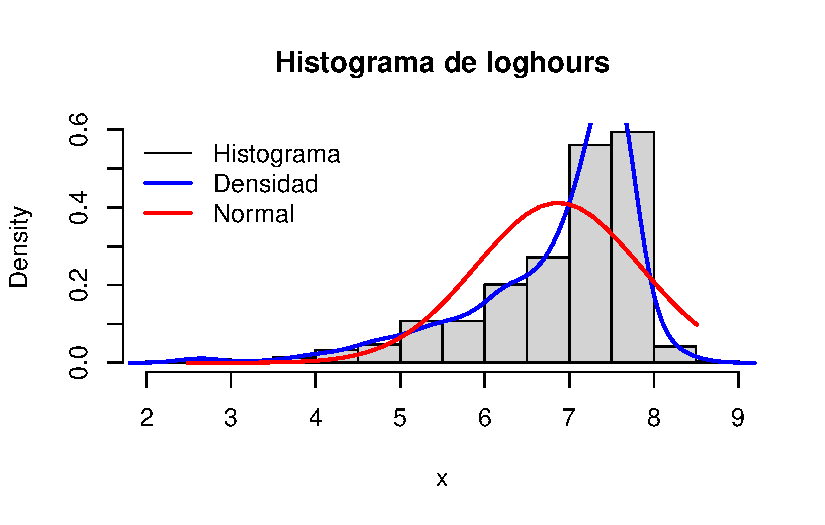
\includegraphics{cap4_files/figure-pdf/lognormal-1.pdf}

Una vez usada la función logaritmo sobre los valores estrictamente
positivos (\(hours>0\)) de la variable \emph{hours}, notamos que la
distribución se acerca a una distribución normal

El comando del modelo de dos partes

\begin{Shaded}
\begin{Highlighting}[]
\FunctionTok{library}\NormalTok{(twopartm)}



\CommentTok{\# Conjunto de variable explicativas necesarias}

\NormalTok{xvars}\OtherTok{\textless{}{-}}\FunctionTok{c}\NormalTok{(}\StringTok{"nwifeinc"}\NormalTok{, }\StringTok{"educ"}\NormalTok{, }\StringTok{"exper"}\NormalTok{, }\StringTok{"expersq"}\NormalTok{, }\StringTok{"age"}\NormalTok{, }\StringTok{"kidslt6"}\NormalTok{, }\StringTok{"kidsge6"}\NormalTok{)}

\NormalTok{fm }\OtherTok{\textless{}{-}} \ControlFlowTok{function}\NormalTok{(y, xvars)\{}
  \FunctionTok{return}\NormalTok{(}\FunctionTok{as.formula}\NormalTok{(}\FunctionTok{paste}\NormalTok{(y, }\StringTok{"\textasciitilde{}"}\NormalTok{, }\FunctionTok{paste}\NormalTok{(xvars, }\AttributeTok{collapse =} \StringTok{"+"}\NormalTok{))))}
\NormalTok{\}}

\CommentTok{\# Se creo una nueva base  de datos con las variables (Provisional)}
\NormalTok{d\_dospartes }\OtherTok{\textless{}{-}}\NormalTok{ mroz }\SpecialCharTok{\%\textgreater{}\%} 
  \FunctionTok{select}\NormalTok{(hours,nwifeinc, educ, exper, expersq, age, kidslt6, kidsge6) }\SpecialCharTok{\%\textgreater{}\%} 
  \FunctionTok{print}\NormalTok{()}
\end{Highlighting}
\end{Shaded}

\begin{verbatim}
    hours    nwifeinc educ exper expersq age kidslt6 kidsge6
1    1610 10.91005993   12    14     196  32       1       0
2    1656 19.49998093   12     5      25  30       0       2
3    1980 12.03991032   12    15     225  35       1       3
4     456  6.79999590   12     6      36  34       0       3
5    1568 20.10005760   14     7      49  31       1       2
6    2032  9.85905361   12    33    1089  54       0       0
7    1440  9.15204811   16    11     121  37       0       2
8    1020 10.90003777   12    35    1225  54       0       0
9    1458 17.30500031   12    24     576  48       0       2
10   1600 12.92500019   12    21     441  39       0       2
11   1969 24.29995346   12    15     225  33       0       1
12   1960 19.70007133   11    14     196  42       0       1
13    240 15.00000763   12     0       0  30       1       2
14    997 14.60000038   12    14     196  43       0       2
15   1848 24.63091469   10     6      36  43       0       1
16   1224 17.53102684   11     9      81  35       0       3
17   1400 14.09998035   12    20     400  43       0       2
18    640 15.83899975   12     6      36  39       0       5
19   2000 14.10000038   12    23     529  45       0       0
20   1324 10.29996109   12     9      81  35       0       4
21   2215 22.65498161   16     5      25  42       0       2
22   1680  8.09004784   12    11     121  30       0       0
23   1600 17.47900009   13    18     324  48       0       0
24    800  9.56000042   12    15     225  45       0       0
25   1955  8.27495289   12     4      16  31       1       1
26    660 27.34998512   17    21     441  43       0       2
27    525 16.00000000   12    31     961  59       0       0
28   1904 16.99998283   12     9      81  32       0       3
29   1516 15.10005569   17     7      49  31       1       0
30    346 15.69998360   12     7      49  42       0       0
31   1040  5.11895990   11    32    1024  50       0       0
32    732 16.75001144   16    11     121  59       0       0
33   1880 13.59993172   13    16     256  36       0       2
34   1680 17.10004807   12    14     196  51       0       1
35   2081 16.73404884   16    27     729  45       0       3
36    690 14.19697762   11     0       0  42       0       1
37   4210 10.31998730   12    17     289  46       0       0
38   2205 11.38410473   10    28     784  46       0       1
39   1952 14.59407806   14    24     576  51       0       0
40   1302 17.50043869   17    11     121  30       0       0
41    112 15.50999641   12     1       1  30       1       2
42    893 21.99997520   12    14     196  57       0       0
43    583 22.50000000   16     6      36  31       1       2
44    480 19.99399948   12    10     100  48       0       2
45   1900 14.13000011   12     6      36  30       0       3
46    576  5.00001287   12     4      16  34       0       2
47   2056 21.15489769   16    10     100  48       0       2
48   1984  7.14194584   12    22     484  45       0       0
49   2640 16.65007210   12    16     256  51       0       0
50    240  6.35199976   12     6      36  30       0       2
51   1173 27.31394768   12    12     144  46       0       1
52   3640 14.50000381   12    32    1024  58       0       0
53    340 16.25798988   12    15     225  37       0       8
54    500  9.50000000    8    17     289  52       0       0
55   1599  7.99995613   10    34    1156  52       0       0
56   1830 12.50002861   16     9      81  31       0       0
57   1920 14.00003242   14    37    1369  55       0       0
58   2052 20.80007362   17    10     100  34       0       0
59   2312 19.38511276   14    35    1225  55       0       0
60    196 12.38699150   12     6      36  39       0       2
61   2500 28.50000000   14    19     361  40       0       3
62   1980 15.04990864   12    10     100  43       0       4
63   1840 10.49998379    8    11     121  48       0       0
64    320 11.81000042   12    15     225  47       0       0
65    419  6.95007324   12    12     144  41       0       4
66   1880 12.41997147    8    12     144  36       0       0
67     72 17.40000343   17    14     196  46       0       2
68    120 15.49999619   12    11     121  34       0       0
69   1885 21.21704292   12     9      81  41       0       3
70    240 18.00000000   12    24     576  51       0       1
71   1729 11.89991856   12    12     144  33       0       0
72   1850 26.75195503   12    13     169  52       0       0
73   2033 12.14996147    9    29     841  58       0       0
74    608 10.19999027   10    11     121  34       2       4
75   1153  8.12001514   12    13     169  31       0       1
76   2208 10.65996456   12    19     361  48       0       1
77    252 18.10000992   12     2       4  32       0       2
78    337  8.59998608   17    24     576  49       0       0
79     90 13.66499996   15     9      81  32       2       2
80   1174 32.34996033   12     6      36  58       0       0
81    372 12.08500576    6    22     484  50       0       0
82     30 12.14999962   14    30     900  60       0       0
83   1800 17.69502068   12    10     100  50       0       1
84    282 24.70000076   14     6      36  56       0       0
85    720  2.13399196    9    29     841  51       0       0
86   1440 20.95004845   17    29     841  54       0       1
87   2100 10.50008011   13    36    1296  59       0       0
88   1000 10.55000019    9    19     361  46       0       2
89    952 45.75000000   15     8      64  46       0       1
90   1413 13.63204002   12    13     169  39       1       3
91   2100 18.23893929   12    16     256  44       0       2
92    120 17.08999634   12    11     121  33       2       0
93   3000 30.23489952   12    15     225  33       1       2
94   1000 28.70000076   12     6      36  48       0       2
95    336 19.62999535   12    13     169  31       0       4
96   1216 12.82494259   12    22     484  45       0       1
97    988 23.79999924   12    24     576  45       0       1
98   2581 26.30002594   13     2       4  32       0       2
99   2030 20.69990730   12     6      36  47       0       0
100   413 26.00000381   13     2       4  34       0       2
101   782 10.87702084   12     2       4  37       0       1
102  1388 25.61206245   12    14     196  36       0       1
103  1450 20.98899460   12     9      81  47       1       2
104  1720 70.74993134   16    11     121  48       0       1
105   800 17.04999924   12     9      81  42       0       2
106   360 20.99999619   13     6      36  33       0       3
107  2000  8.11999989   11    19     361  46       0       0
108  1176 20.88599014   12    26     676  47       0       3
109  2058 17.66891861   12    19     361  44       0       1
110   900 25.20002937   12     3       9  36       0       4
111   215 14.24500561   17     7      49  31       2       0
112  2000 14.30000019   14    28     784  55       0       0
113   757 23.70001030   16    13     169  45       0       1
114  1264 45.99999619   17     9      81  47       0       0
115  2064 42.99990463   12    15     225  46       0       3
116  1280 14.74899960   11    20     400  49       0       0
117  1715 16.15005493   12    29     841  49       0       0
118  2000 17.77400017   12     9      81  45       0       2
119    12 91.00000000   17     1       1  38       1       3
120  1528 22.29993439   10     8      64  47       0       0
121   561 34.60001373   13    19     361  54       0       3
122  2058  9.62000179   11    23     529  41       0       0
123  1823 10.89994621   12     3       9  43       0       2
124  1680 14.49994373   16    13     169  31       1       1
125  1440 22.00001526   17     8      64  47       0       0
126  4950 17.90007973   12    17     289  35       0       2
127  1176 23.67506218   16     4      16  45       0       3
128  1100 11.79996014   12    15     225  33       1       0
129  1516 16.14195442   16    11     121  54       0       1
130   900 18.39997101    8     7      49  35       0       4
131  1080 15.49994755   12     0       0  31       1       2
132   480 17.32399940   12     0       0  55       0       0
133   288 19.20500374   12    10     100  34       0       2
134  1875 21.30006218   13     8      64  38       0       1
135   630 23.55999565   11     2       4  45       0       1
136   234 20.85000038   12     4      16  47       0       1
137  1600 26.14999962   12     6      36  39       0       2
138   960 17.00000000   14    18     324  36       1       0
139   120 20.72000313   12     3       9  33       1       2
140  2025 17.00008965   12    22     484  50       0       0
141  1809 15.99999809   12    33    1089  58       0       0
142  3087 19.50004959   17    28     784  49       0       0
143   910 12.00000381   14    23     529  41       0       2
144  1840 13.73191166   12    27     729  51       0       1
145   784 27.19999123    9    11     121  53       0       0
146   400  5.31500006   12     6      36  36       1       2
147  1000 16.00000000   12    11     121  46       0       2
148  1904 27.87198257   12    14     196  36       0       2
149  1771 40.00001144   14    17     289  53       0       1
150  1486 15.90003395   16    17     289  40       0       3
151   740 27.49996948   17    14     196  42       0       2
152  1820 17.02005005   15    11     121  33       1       1
153  1275 22.39493942   12     7      49  43       0       3
154   450 11.10000038   16     8      64  31       1       0
155  1221 32.70001221   17     6      36  47       0       0
156  1550 27.79996109   17     8      64  54       0       0
157   180  2.19999409   12     4      16  33       1       3
158  2090 19.72095108   16    25     625  43       0       0
159  1960  9.99998760   13    24     576  46       0       1
160  1440 13.19996834   12    11     121  35       0       3
161   794 12.70897484   11    19     361  37       0       3
162   993 27.30004692   16     9      81  37       0       2
163   160 21.20000076   14    19     361  34       0       3
164   105 14.40000439   16    14     196  43       1       0
165  1200 20.57596016   12    22     484  46       0       0
166   450 12.49999046    9     6      36  35       0       3
167   996 17.50021553   17    23     529  46       0       0
168  1052 44.00003815   14    15     225  46       0       0
169  1128 13.11895466   12     6      36  43       0       2
170  1840 14.00005627   12    11     121  30       0       0
171  1910  9.64508629   11     2       4  41       0       2
172   980 17.39704514   12    22     484  54       0       1
173  2317  7.79988861   12    10     100  31       0       1
174  1089 13.13397694   10    14     196  44       0       0
175   800 25.60000038   12    12     144  32       0       1
176  1230 13.90002537    5     9      81  47       0       0
177  1158 19.29794312   17    13     169  46       0       1
178  2272  9.20001602   11    18     324  37       0       0
179   528 37.99998856   12     8      64  51       0       2
180  1000 44.00000000   12    11     121  49       0       1
181   520 21.37202454   14     9      81  36       0       4
182   760 23.66802025   11     9      81  39       0       1
183  1920  9.00000000   12    14     196  48       0       2
184  1220 25.19995117   14     9      81  38       0       2
185   200 21.21999931   12     2       4  40       0       2
186  2480 33.96991348   10    12     144  39       1       5
187  2750 17.06999969   16    15     225  37       0       0
188  2014  6.01602364   13    11     121  49       0       1
189  1355 17.10000992   12     7      49  33       0       3
190    80  8.23700047   12     9      81  30       0       0
191  1670 13.30008221   12    19     361  54       0       0
192   520 16.00002098   11    11     121  39       0       4
193   288 12.53999043   12     8      64  43       0       3
194  2014 18.00003815    9    13     169  31       0       3
195   800 31.20000076   13     4      16  33       0       3
196  1984 20.74991035   12     7      49  40       0       3
197  1823 11.09992027   12    19     361  36       0       1
198  1500 20.68000031   12    14     196  51       0       0
199  2261 18.00000954   13    14     196  44       0       1
200  1728 32.43006516   16     3       9  42       0       3
201  1960 32.90003204   12     9      81  40       0       1
202  1578 24.10000610   16     7      49  34       1       1
203  1316 17.80039215   17     7      49  30       0       0
204  1530 20.50001717   12    14     196  54       0       0
205  2220 10.49989796   12    29     841  51       0       0
206  1336 10.43703461    9    19     361  44       0       2
207  1008 18.19499016   12    14     196  43       0       1
208  1944 12.84507656   12    16     256  34       0       1
209  2000 13.80000019   13    10     100  45       0       0
210   258 22.19999504   12    12     144  39       0       0
211  1785  6.69994116   12    24     576  50       0       0
212   480  6.25001574   12     6      36  52       0       0
213   772 15.60000801   12     9      81  41       0       2
214   900  3.30000997   10    14     196  59       0       0
215  1428  3.67097759   12    26     676  52       0       0
216   210  7.78999710   16     7      49  46       0       0
217   239 18.27198982   12     4      16  41       1       5
218  1878 10.95397949   11    15     225  33       0       2
219   215 13.49999237   12    23     529  45       0       0
220  2340 11.20001221   10     1       1  36       1       2
221  1960 20.99990845   12    29     841  48       0       1
222   532 25.69999886   12     9      81  47       0       1
223   394  8.93299389   12     6      36  45       0       0
224   675 19.15997696   12    11     121  37       0       2
225  1515 26.58998680   16    17     289  46       0       4
226  1030 22.40000534   17     6      36  43       0       3
227  1250 20.63299942   12     7      49  42       0       2
228  1158 28.20000648   17     2       4  34       1       2
229   112 28.79999924   12    24     576  52       0       0
230   336  8.99999714   12     4      16  37       0       3
231  1984 11.39994240   12    11     121  37       0       1
232   716 10.40001392    8    25     625  52       0       0
233  1410 19.08005524   12    11     121  30       1       0
234  1300  9.46603966   13     2       4  31       0       1
235  1640  6.50006008   12    19     361  38       0       1
236  1202 29.11701393   12     7      49  43       0       3
237   489 19.10301971    8     2       4  49       0       1
238  2076 16.34997177   12    20     400  55       0       0
239   526 32.02501678   17    10     100  38       0       2
240  1721 16.70006180   17    19     361  52       0       0
241  1327  4.81103754   12    17     289  48       0       0
242   584 24.62600899   13    12     144  32       0       2
243  1376 17.40001297   12    11     121  32       0       1
244  1040 13.02503967   12     6      36  38       0       2
245   548 19.00698280   12    10     100  46       0       3
246    15 14.02999973   12     4      16  40       0       3
247  1980 14.89990616    9     2       4  31       0       4
248  1520 25.00005531   10    13     169  43       0       1
249  1880 10.70006752   12    21     441  51       0       0
250  1260 24.25000381   16     9      81  30       1       0
251  1092 39.13996506   13     4      16  52       0       0
252  1587  7.19997311    8     2       4  30       1       5
253   156 31.81099892   16    19     361  51       0       0
254  1939 10.00004768   13     4      16  31       0       2
255  1250 20.65999985   12     9      81  34       0       4
256   610 13.49997616   11    14     196  49       0       0
257   270 25.37999535   13     6      36  35       1       3
258   660 18.27497673   12    24     576  53       1       0
259  1000 39.21300125   12     1       1  32       0       3
260  1920 10.49993610   10    13     169  38       0       3
261   200 34.85699844   12     3       9  54       0       0
262  1500 28.50199890   17    10     100  47       0       1
263   868 12.99995995   15    16     256  45       0       1
264  2318 41.39990997   16     9      81  47       0       1
265  2000 14.77999973   10    19     361  59       0       0
266    60 15.04999828   11     4      16  32       0       1
267  1715 29.69997787   12    10     100  45       0       1
268   550 16.16501999   12     5      25  40       0       4
269  1960 25.20515823   14     7      49  47       0       2
270    44 14.19999886   16     3       9  36       1       2
271  1920 18.15896797   14    38    1444  56       0       0
272  2540 28.98106384    8    16     256  41       0       1
273   156 13.39200306    7    13     169  48       0       3
274   780  9.17502022   12     1       1  36       1       2
275  3120 27.03984833   12     7      49  41       0       0
276  2040 13.14995193   14    15     225  41       0       0
277  1610 16.40007019   12    10     100  36       0       3
278   215 21.29999161   12     2       4  37       0       3
279  1120 17.20101547   12    19     361  38       0       0
280   846  8.56002617   14    25     625  43       0       2
281  3225  6.49083996   16    25     625  54       0       0
282  1376 12.49996758   12     7      49  38       0       1
283   980 27.00002480   12    15     225  30       1       0
284  1838 53.50004959   12    11     121  49       0       0
285  1494 52.49994659   13    25     625  45       0       1
286   450 38.39997864   13    19     361  51       0       0
287  1976 13.89194489   10     4      16  34       0       0
288  2012  3.89999294   12    14     196  34       0       2
289   561 34.19999695   12    19     361  41       0       1
290  1715 19.70007896   12    18     324  49       0       1
291  1912 18.49995232   12    14     196  32       0       0
292  3686 10.99997616   14    11     121  32       0       0
293  1080 43.30001068   17     4      16  32       0       2
294  1799 18.76000786   10    29     841  47       0       0
295  1984  4.80009604    9    21     441  39       0       1
296  1839 21.50000191   12    24     576  49       0       0
297  1579 28.03993797   12    19     361  37       0       3
298    96 26.00000381   16    31     961  59       0       0
299  1920 27.00000000   12    28     784  50       0       0
300  1688 17.79968834   17    15     225  32       0       1
301  1589 17.40194511   12    27     729  46       0       0
302   345 19.30999184   17    13     169  43       0       2
303  1521  9.99997997   11     4      16  37       0       3
304  1490 11.17998028   16    10     100  32       0       2
305   989 18.85695648   11     8      64  39       0       1
306   600 12.30002022   13     4      16  34       0       2
307  2646 13.67711830   11    18     324  39       0       1
308  2149  9.55999660    8     3       9  45       0       3
309   320 24.49998474   11    11     121  50       0       0
310  1600 23.14999962   12     8      64  40       0       1
311  2419 15.59088326   10    10     100  30       0       1
312  2005 14.42092419   17    33    1089  57       0       0
313  1960 17.45490837   12    19     361  39       0       1
314  2147  9.80001926   12    35    1225  53       0       0
315  1207 17.57446480   17    21     441  48       0       1
316  2000 16.55500031   14     7      49  46       0       1
317  1260 13.29497433   12    18     324  47       0       0
318    90 11.84400272   12     4      16  43       0       1
319  1800 46.64506149   12    12     144  47       0       0
320   573 14.69998932   12    16     256  47       0       1
321  1825 26.09008026   12    14     196  47       0       0
322    75  9.89999962   12     3       9  46       0       0
323  1348  9.04802608    9     1       1  34       0       4
324  1880 30.75006485   10    27     729  48       0       0
325  1240  8.49993992   12    12     144  30       0       1
326   848 22.24999237   12     6      36  51       0       1
327   150 42.90999985   12     9      81  52       0       5
328  2000 33.29999924   12     2       4  37       0       2
329  1952 13.81990337   12     6      36  32       0       2
330  1456 23.60000801   17     9      81  36       0       2
331  1740 13.00006771   12    16     256  35       0       2
332  1400 20.74994087   17    22     484  45       0       0
333  2000  6.30000019   12    26     676  56       0       0
334  1750  7.78892469   10    11     121  40       0       2
335  1101 10.47004032   12    11     121  45       1       2
336  2000 12.00000000   12    15     225  32       0       2
337  1877 16.97991562   12    13     169  45       0       0
338   160 17.89999962   12     6      36  40       0       2
339  1886 15.53993702   12    20     400  38       0       1
340  1446  9.88398552   12    17     289  49       0       4
341  1500 28.59995079   16     8      64  47       0       1
342   860 17.66001129   13    13     169  52       0       0
343  1848 25.99991798   13    15     225  34       0       1
344  1678 13.60200977   12    14     196  44       0       2
345   160 15.80000019   16    14     196  36       0       3
346   108 41.09999466   17     6      36  50       0       0
347  1738 10.77504158   12    24     576  45       0       0
348  1170  9.00004673   14    10     100  44       0       2
349    15 24.39899445   12     2       4  57       0       2
350  2088 37.30009079   17     9      81  35       0       0
351  2490 27.99994850   12    23     529  46       0       0
352   135 13.70000267   14    12     144  30       2       1
353  1944 17.20994377   12     8      64  42       0       3
354   690 14.00001431   12    16     256  34       0       1
355   608 35.75502014   17    10     100  45       0       2
356    63 23.49999619   16     7      49  35       1       2
357   154 31.99993324   16    19     361  40       0       0
358   420 17.14999580   12     2       4  32       0       1
359   651 20.25002480    9     9      81  54       0       0
360   675  5.48598480   12    14     196  38       0       3
361  1663 25.07504082   12     9      81  43       0       3
362  1680 18.21995163   16    16     256  54       0       0
363   180 25.99999619   14     7      49  39       0       3
364  1581 34.50007248   12     6      36  37       0       1
365  1200 12.39999962   12    22     484  46       0       2
366   450 10.78684998   11     9      81  56       0       0
367   547 16.32300758   12     9      81  41       0       3
368   300 30.50000000   16    14     196  45       0       1
369   975 51.29962540   17    17     289  44       0       1
370  1621 33.04997253   17    12     144  50       0       1
371   300 34.75001144   14    13     169  37       0       5
372  1868 16.40003967   12     8      64  44       0       1
373  1803 19.70007324   14    10     100  32       0       2
374  2143  6.60000277   12    16     256  34       1       1
375  1080  9.02000809   10     1       1  32       0       2
376  1352 10.40000820   12     6      36  37       0       3
377   537 14.51998806   13     4      16  44       0       1
378   352 17.19999695   16     8      64  34       0       2
379   200 43.00000000   12     4      16  33       1       3
380  2045 13.87195969    7    15     225  43       0       3
381  1253 -0.02905745   16     7      49  35       0       2
382  1960 16.76994324   14    14     196  43       0       1
383  2000  7.79999971   12    16     256  34       0       0
384  1960 14.50006390   10    15     225  36       0       3
385  2000  7.90000010   12    23     529  41       0       2
386  1568 79.80001068   16    19     361  41       0       0
387  1225  7.17597008   10     4      16  35       0       3
388   780 17.50698280   12    12     144  32       1       3
389   480 20.60000038   14    12     144  30       0       0
390  1923 18.55991554   12    25     625  43       0       0
391  2000  9.30000019    6    14     196  54       0       0
392  2110  5.12000751   15    14     196  35       0       2
393  1664 14.50003815   12    11     121  50       0       0
394    48 19.79999924   17     7      49  34       1       1
395  1791 18.29994965   14    18     324  52       0       0
396  1404 33.99993515   13     4      16  35       0       3
397  1920 11.62793636    6    37    1369  55       0       0
398  2141 11.80004597   16    13     169  35       0       0
399  1720 39.09997559   14    14     196  49       0       1
400  3533 18.43007088   15    17     289  38       2       2
401  2000 21.00000000   14     5      25  42       0       2
402   800 59.00000000    8     2       4  48       0       1
403  3000 25.29999924   14     0       0  51       0       0
404   293 23.24899101   12     3       9  43       0       2
405  1872 24.92808723   12    21     441  43       0       1
406  2058 14.78198814   12    20     400  38       0       1
407  1832 18.90002823   12    19     361  44       0       1
408   120 21.00000000   12     4      16  36       1       3
409  1632 10.00000954   12    19     361  38       0       0
410   778 29.30997467    8    11     121  47       0       0
411  1984 13.14003181   12    14     196  34       0       2
412   225 25.08999443   17     8      64  40       1       2
413  1960 14.59993172   12    13     169  31       0       1
414   444  1.20000124   12    24     576  46       0       0
415   384 32.00000381   14     1       1  36       0       3
416  1170 16.11997032   13     1       1  39       1       2
417  1330 26.50002289   17     3       9  36       0       2
418  1350 12.75005531    8     4      16  37       0       4
419   480 12.89999962   12    21     441  39       0       4
420  1984 10.69997501   11    10     100  36       1       3
421  1944 14.43403149   12    13     169  49       0       2
422    50 23.70899963   12     9      81  45       1       1
423   460 15.10000420   17    14     196  32       2       0
424   680 18.19997597   10     2       4  36       0       5
425  2450 22.64105606   12    21     441  40       0       1
426  2144 21.64007950   13    22     484  43       0       2
427  1760 23.99998474   12    14     196  33       0       1
428   490 16.00001526   12     7      49  30       0       1
429     0 21.02499962   12     2       4  49       0       1
430     0 23.60000038   16     5      25  30       2       0
431     0 22.79999924   12    12     144  30       1       0
432     0 35.90999985   12     1       1  41       0       4
433     0 21.70000076   12    12     144  45       0       1
434     0 21.82299995   12     4      16  43       0       5
435     0 31.00000000   13     9      81  42       0       1
436     0 15.30000019   12     9      81  60       0       0
437     0 12.92500019   12     6      36  57       0       0
438     0 15.82999992   10     5      25  38       0       2
439     0 30.20000076   12     5      25  56       0       0
440     0 16.60000038   12     8      64  32       0       3
441     0 11.00000000    7     2       4  49       0       1
442     0 15.00000000   12     6      36  55       0       0
443     0 20.52799988    9     0       0  36       1       1
444     0 13.12600040   12     3       9  44       0       3
445     0 15.55000019   10     7      49  44       0       1
446     0 18.01000023   14     3       9  35       1       2
447     0 18.87400055   14    10     100  44       2       3
448     0 24.79999924   12     3       9  45       0       1
449     0 17.50000000   12     2       4  34       1       0
450     0 16.14999962   17    12     144  30       2       0
451     0 15.18900013    8    15     225  39       0       1
452     0  6.00000000   12     5      25  36       0       2
453     0 37.25000000   17     4      16  38       0       2
454     0 27.76000023   12    10     100  53       0       0
455     0  9.09000015   12     1       1  36       0       2
456     0 14.50000000   12     8      64  32       1       1
457     0 19.70000076    9    20     400  51       0       3
458     0 16.78800011   11     4      16  38       0       0
459     0 18.52000046   12     7      49  33       2       0
460     0 20.95000076   12    10     100  54       0       0
461     0  7.57399988    9     3       9  38       0       3
462     0 10.02700043   11     5      25  30       2       2
463     0  5.00000000   12    10     100  34       2       3
464     0  7.03999996    9     0       0  34       0       1
465     0 40.79999924   12     3       9  50       0       2
466     0 16.04999924   17    10     100  30       2       0
467     0 33.09999847   12     2       4  38       0       2
468     0 33.85599899   14    10     100  54       0       0
469     0 20.50000000   12     4      16  30       1       2
470     0 28.60000038   12     0       0  55       0       0
471     0 18.75000000   10    10     100  51       0       1
472     0 20.29999924   12     5      25  44       0       1
473     0 13.42000008   12     0       0  53       0       0
474     0 18.39999962   10     0       0  42       0       2
475     0 16.68199921   12    19     361  38       0       2
476     0 32.68500137   13     2       4  38       1       3
477     0  7.05000019   12    12     144  41       1       4
478     0 10.86699963    8     5      25  35       0       3
479     0 18.21999931   12     5      25  33       1       2
480     0 26.61300087   13     5      25  48       0       0
481     0 25.00000000   12    10     100  47       0       0
482     0 15.69999981   12     0       0  34       0       5
483     0 40.25000000   13     4      16  33       2       1
484     0 73.59999847   13     3       9  31       3       1
485     0 10.59200001    8     2       4  58       0       0
486     0  8.00000000   12     1       1  49       0       0
487     0 13.39999962    8     0       0  55       0       1
488     0 23.70000076   14     1       1  44       0       0
489     0 18.89999962    9     1       1  44       0       0
490     0 48.29999924   16     6      36  36       0       3
491     0 24.46999931   12    12     144  38       0       3
492     0 28.62999916   16     6      36  37       0       3
493     0 25.31999969   12     9      81  47       0       0
494     0 13.52999973   12    14     196  47       0       3
495     0 14.80000019   12    13     169  32       1       1
496     0 17.39999962   12     8      64  43       1       2
497     0 15.97999954   11     0       0  42       1       4
498     0 16.57600021   12     1       1  56       0       0
499     0 21.85000038   13     3       9  38       0       5
500     0 14.60000038   12    13     169  52       0       2
501     0 21.60000038   12     3       9  50       0       0
502     0 24.00000000   16     8      64  33       0       0
503     0 20.88299942   16     8      64  44       0       2
504     0 19.50000000   12    18     324  41       0       1
505     0 42.79999924   12     2       4  45       0       1
506     0 41.50000000   14     3       9  53       0       0
507     0 18.96500015   14     5      25  53       0       0
508     0 16.10000038   12     2       4  42       0       1
509     0 14.69999981   13    10     100  32       2       0
510     0 18.79999924   12    30     900  56       0       0
511     0 14.75000000   11     1       1  37       1       3
512     0 21.00000000   12     5      25  40       1       2
513     0 35.40000153   15     8      64  54       0       3
514     0 10.69999981    7     0       0  53       0       0
515     0 24.50000000   12     4      16  48       0       1
516     0 17.04500008   12     2       4  36       1       2
517     0 18.79999924   12    30     900  57       0       0
518     0 14.00000000   12    25     625  51       0       0
519     0 18.21400070   13     3       9  33       0       4
520     0 20.17700005   12    20     400  52       0       0
521     0  8.30000019   10    20     400  56       0       0
522     0 14.19999981   12     0       0  36       1       2
523     0 21.76799965   14    15     225  36       1       0
524     0 29.55299950   12    10     100  46       0       1
525     0  4.34999990   10     4      16  31       0       3
526     0 24.00000000   11     3       9  52       0       0
527     0 18.29999924   12    10     100  46       0       2
528     0 17.20000076   12     9      81  35       2       0
529     0 16.47599983   12     7      49  59       0       0
530     0 13.39999962    8    12     144  36       0       1
531     0 44.98799896    7     0       0  51       1       3
532     0 18.20000076   16    16     256  31       1       0
533     0 28.00000000   14     4      16  31       0       2
534     0 11.55000019   12     7      49  32       1       1
535     0 28.45000076   16     7      49  35       1       2
536     0 15.09599972   12    14     196  40       0       3
537     0  8.00899982   10     2       4  33       1       2
538     0 10.03999996    7    20     400  54       0       0
539     0 16.70000076   12     5      25  36       1       1
540     0  8.39999962   10    10     100  50       0       1
541     0 13.00000000    8    20     400  54       0       0
542     0 17.96999931   11    10     100  48       0       1
543     0 18.45000076   15     8      64  41       0       4
544     0 31.00000000   12    11     121  50       0       4
545     0 24.13500023   12     3       9  46       0       2
546     0 31.70000076   13     6      36  42       0       1
547     0 10.18999958    9     4      16  31       1       2
548     0 21.57399940   12     4      16  53       0       0
549     0 26.68000031   12     9      81  51       0       1
550     0 17.70000076   12    10     100  47       0       1
551     0 29.39999962   12     3       9  50       0       1
552     0 22.15900040    6     2       4  37       0       1
553     0 35.00000000   12     2       4  30       2       2
554     0  8.63000011   12     0       0  49       0       0
555     0 17.07999992   12     8      64  52       0       2
556     0 32.50000000   12     6      36  47       0       2
557     0 16.00000000   12    15     225  49       0       0
558     0 18.85000038   12    15     225  44       0       4
559     0 17.50000000    8     9      81  53       0       0
560     0 19.39200020   12     8      64  30       1       0
561     0 14.44999981   12    18     324  54       0       2
562     0 21.79999924    7     3       9  47       1       1
563     0  7.69999981   15    10     100  56       0       0
564     0 31.79999924   12     6      36  49       0       1
565     0 17.25799942    6    20     400  48       0       0
566     0 13.39900017   12     8      64  49       0       1
567     0 16.07299995   12     3       9  56       0       1
568     0 23.26000023   12     4      16  46       0       0
569     0 37.29999924   12    13     169  45       0       2
570     0 11.00000000   12     4      16  32       0       2
571     0 13.07499981   12    17     289  43       1       1
572     0 13.69999981   12     4      16  34       1       1
573     0 25.10000038   12     0       0  30       1       1
574     0 18.60000038   17    15     225  38       2       0
575     0 29.00000000   16    11     121  33       1       1
576     0 19.23699951   12    23     529  52       0       0
577     0 19.85499954   11     1       1  43       0       3
578     0  9.44999981   12     5      25  33       1       1
579     0 30.00000000   10     1       1  45       0       0
580     0 15.00000000   10     5      25  36       2       1
581     0 24.70100021   12     3       9  34       1       1
582     0 15.89999962   14     3       9  37       0       2
583     0 16.23999977   10    19     361  46       0       1
584     0 21.10000038   12    20     400  47       0       0
585     0 23.00000000   16     5      25  31       2       1
586     0  6.34000015    5     0       0  57       0       0
587     0 42.25000000   12     3       9  30       1       1
588     0 14.69400024   12     3       9  30       0       0
589     0 21.41699982   12     7      49  44       0       3
590     0 20.20000076   13     7      49  53       0       0
591     0 12.09000015    8     1       1  51       0       0
592     0 24.76000023   12    13     169  39       1       3
593     0 23.00000000    8     0       0  52       0       0
594     0 19.36499977    8     0       0  46       0       4
595     0  5.55000019   12    12     144  47       0       5
596     0 68.03500366    8     0       0  52       0       2
597     0 29.29999924   12     5      25  45       0       2
598     0 18.50000000   11    45    2025  60       0       0
599     0 22.58200073   13    10     100  41       0       2
600     0 21.50000000    8     2       4  39       0       3
601     0 28.06999969   12     3       9  49       0       1
602     0 50.29999924   15     1       1  32       1       1
603     0 23.50000000   12     5      25  33       1       3
604     0 15.50000000   10    10     100  36       0       4
605     0 13.43999958   13     4      16  37       3       3
606     0  8.10000038   12     7      49  30       1       2
607     0  9.80000019   11     9      81  44       1       1
608     0 20.29999924   12     5      25  48       0       1
609     0 15.00000000   11     4      16  40       0       4
610     0 56.09999847   13    11     121  47       0       0
611     0 22.84600067   12     9      81  36       0       2
612     0 22.22500038   11     4      16  40       0       2
613     0 17.63500023   12     2       4  46       0       1
614     0 18.50000000   12    23     529  52       0       0
615     0 13.39000034   12     3       9  44       0       1
616     0 15.14999962   10    15     225  45       0       1
617     0 16.20000076    7     8      64  30       2       1
618     0 33.91999817   12     3       9  40       1       3
619     0 14.00000000   12    25     625  43       0       1
620     0 16.73600006   12     2       4  49       0       2
621     0 30.64999962   12     0       0  46       1       4
622     0 12.39999962   11    19     361  52       0       0
623     0 19.02199936   12     3       9  31       1       1
624     0 11.20300007   10     7      49  42       1       1
625     0 19.87599945   11     1       1  33       0       3
626     0 57.00000000   16     9      81  57       0       0
627     0 18.29000092   10     3       9  49       0       0
628     0 20.21999931   14     8      64  45       0       1
629     0 22.14999962   11     0       0  56       0       0
630     0 30.62299919   12     5      25  41       1       3
631     0  9.38000011    5    20     400  56       0       0
632     0 22.00000000   10     3       9  48       0       1
633     0 23.67499924   16    12     144  52       0       2
634     0 33.67100143   12     5      25  51       0       0
635     0 12.36699963   11     1       1  35       0       3
636     0 21.95000076   12     0       0  45       0       0
637     0 32.00000000   12     7      49  54       0       0
638     0 22.61000061   12    13     169  54       0       2
639     0 12.09200001   12     3       9  31       1       0
640     0  3.77699995    6     0       0  53       0       3
641     0 36.00000000   14     2       4  35       2       2
642     0 26.89999962   12     0       0  36       1       3
643     0 32.24200058   12     2       4  59       0       0
644     0 35.02000046   16     1       1  54       0       0
645     0 37.59999847   12    10     100  37       1       1
646     0  1.50000000   12    10     100  44       0       0
647     0 96.00000000   17     1       1  34       1       2
648     0 18.14999962   12     3       9  49       0       0
649     0 15.50000000   12    32    1024  49       0       0
650     0 14.00000000    9     0       0  60       0       0
651     0 14.75599957   12     7      49  51       0       0
652     0 22.00000000   12     5      25  30       1       1
653     0 24.46599960   12     2       4  47       0       2
654     0 24.39999962   12     5      25  36       0       4
655     0 24.00000000   12     3       9  35       1       3
656     0 15.50000000   12    25     625  58       0       0
657     0 30.79999924   14     0       0  41       1       3
658     0 10.65999985   10     3       9  51       0       1
659     0 13.35000038   12    10     100  47       0       0
660     0 10.09000015    9    10     100  45       1       2
661     0 55.59999847   14     7      49  60       0       0
662     0 25.70000076   16     5      25  30       1       1
663     0 29.00000000   11    15     225  55       0       0
664     0  7.28599977   12     1       1  32       1       2
665     0 37.75199890   12     5      25  36       0       2
666     0 13.07199955   12     9      81  55       0       0
667     0  7.04400015   12    18     324  47       0       0
668     0 18.20000076   12     1       1  47       0       1
669     0 27.00000000   11     0       0  37       0       1
670     0 30.29999924   12     6      36  50       0       2
671     0 12.00000000   12     1       1  30       0       3
672     0 31.50000000   17     2       4  48       0       1
673     0 27.09199905   10    15     225  43       0       2
674     0 20.96800041   11    25     625  48       1       0
675     0 27.00000000   14     1       1  41       1       2
676     0 11.22500038   12     0       0  50       0       0
677     0 37.70000076    8     0       0  58       0       0
678     0 28.20000076   13     0       0  38       0       5
679     0 34.00000000   12     8      64  37       0       1
680     0 63.20000076   16    22     484  50       0       0
681     0  7.50000000    8     5      25  42       0       4
682     0 17.40999985    9    10     100  37       1       3
683     0 51.00000000   16     1       1  41       0       2
684     0 12.91600037   12     1       1  31       0       2
685     0 21.89999962   12     6      36  51       0       0
686     0 17.63999939   12     4      16  36       1       2
687     0 20.00000000   15     6      36  54       0       0
688     0 15.00000000   12     0       0  49       0       0
689     0 14.06000042    9     1       1  48       1       1
690     0 15.82499981    9     3       9  42       0       2
691     0 16.51000023   12    15     225  41       1       2
692     0 13.00000000   16    33    1089  55       0       0
693     0 10.00000000    9     2       4  42       0       0
694     0 22.00000000   15     1       1  32       0       1
695     0 29.79999924   12    10     100  43       0       2
696     0 15.00000000   12     0       0  33       1       3
697     0 22.29999924   15    14     196  48       0       1
698     0 14.55000019   12    15     225  43       0       2
699     0 19.72999954   17    15     225  47       1       3
700     0 35.00000000   12    10     100  54       0       0
701     0 21.01399994   12     6      36  51       0       1
702     0 10.87600040   10    18     324  51       0       1
703     0 27.85000038   13    15     225  43       1       1
704     0  9.56000042   12    30     900  53       0       0
705     0 30.29999924   11    15     225  34       1       1
706     0  7.71999979    8    10     100  31       1       1
707     0 10.55000019   12     0       0  56       0       0
708     0 24.10600090   16     0       0  42       0       1
709     0 22.99500084   12     4      16  32       0       2
710     0  6.00000000   12     0       0  35       1       3
711     0 24.35000038   12     3       9  30       1       1
712     0  7.60799980   10    20     400  51       0       0
713     0 28.20000076   12     3       9  47       0       3
714     0 16.14999962   12     1       1  54       0       1
715     0 51.20000076   15     5      25  31       3       0
716     0 12.64599991   10     7      49  47       0       0
717     0 19.00000000   14     6      36  47       0       3
718     0 19.00000000   12     2       4  40       0       3
719     0 14.39999962    8     0       0  48       0       0
720     0  7.23199987    8    10     100  34       0       7
721     0 21.94300079   12     6      36  38       0       3
722     0 47.50000000   12     4      16  32       1       3
723     0 28.89999962   16     8      64  48       0       1
724     0 12.39999962   12    18     324  41       0       2
725     0  6.53100014    5     7      49  49       0       2
726     0 22.42200089    8    15     225  59       0       0
727     0 22.20000076   13     7      49  58       0       0
728     0 77.00000000   12     8      64  41       0       3
729     0 88.00000000   12     8      64  45       0       2
730     0 26.04000092   14     3       9  30       1       1
731     0 63.50000000   12    10     100  41       0       1
732     0 12.10000038   12     9      81  30       2       0
733     0 17.50499916   12    24     576  53       0       1
734     0 18.00000000   12    12     144  31       0       0
735     0 28.06900024   14     2       4  43       0       2
736     0 14.00000000   12     6      36  31       1       1
737     0  8.11699963   12    18     324  51       0       0
738     0 11.89500046    9    17     289  43       0       0
739     0 45.25000000   14     7      49  31       1       2
740     0 31.10600090   11     6      36  48       0       0
741     0  4.00000000   12    10     100  31       1       1
742     0 40.50000000   12     5      25  44       0       1
743     0 21.62000084   11     7      49  48       0       1
744     0 23.42600060   12    11     121  53       0       1
745     0 26.00000000   10    14     196  42       0       3
746     0  7.84000015   12     5      25  39       2       6
747     0  6.80000019   10     2       4  32       1       2
748     0  5.32999992   12     4      16  36       0       2
749     0 28.20000076   13     5      25  40       0       2
750     0 10.00000000   12    14     196  31       2       3
751     0  9.95199966   12     4      16  43       0       0
752     0 24.98399925   12    15     225  60       0       0
753     0 28.36300087    9    12     144  39       0       3
\end{verbatim}

\begin{Shaded}
\begin{Highlighting}[]
\NormalTok{mode}\FloatTok{.2}\NormalTok{p }\OtherTok{\textless{}{-}} \FunctionTok{tpm}\NormalTok{(}\FunctionTok{fm}\NormalTok{(}\StringTok{"hours"}\NormalTok{, xvars),}
               \AttributeTok{data =}\NormalTok{ mroz,}
               \AttributeTok{link\_part1 =} \StringTok{"logit"}\NormalTok{, }
               \AttributeTok{family\_part2 =} \FunctionTok{Gamma}\NormalTok{(}\AttributeTok{link =} \StringTok{"log"}\NormalTok{))}

\FunctionTok{summary}\NormalTok{(mode}\FloatTok{.2}\NormalTok{p)}
\end{Highlighting}
\end{Shaded}

\begin{verbatim}
$Firstpart.model

Call:
glm(formula = nonzero ~ nwifeinc + educ + exper + expersq + age + 
    kidslt6 + kidsge6, family = binomial(link = "logit"), data = mroz)

Coefficients:
             Estimate Std. Error z value Pr(>|z|)    
(Intercept)  0.425452   0.860365   0.495  0.62095    
nwifeinc    -0.021345   0.008421  -2.535  0.01126 *  
educ         0.221170   0.043439   5.091 3.55e-07 ***
exper        0.205870   0.032057   6.422 1.34e-10 ***
expersq     -0.003154   0.001016  -3.104  0.00191 ** 
age         -0.088024   0.014573  -6.040 1.54e-09 ***
kidslt6     -1.443354   0.203583  -7.090 1.34e-12 ***
kidsge6      0.060112   0.074789   0.804  0.42154    
---
Signif. codes:  0 '***' 0.001 '**' 0.01 '*' 0.05 '.' 0.1 ' ' 1

(Dispersion parameter for binomial family taken to be 1)

    Null deviance: 1029.75  on 752  degrees of freedom
Residual deviance:  803.53  on 745  degrees of freedom
AIC: 819.53

Number of Fisher Scoring iterations: 4


$Secondpart.model

Call:
glm(formula = hours ~ nwifeinc + educ + exper + expersq + age + 
    kidslt6 + kidsge6, family = Gamma(link = "log"), data = mroz)

Coefficients:
              Estimate Std. Error t value Pr(>|t|)    
(Intercept)  7.7164988  0.2928967  26.345  < 2e-16 ***
nwifeinc    -0.0003793  0.0030546  -0.124 0.901231    
educ        -0.0191886  0.0138927  -1.381 0.167951    
exper        0.0427191  0.0123052   3.472 0.000571 ***
expersq     -0.0005876  0.0003697  -1.589 0.112732    
age         -0.0148794  0.0049825  -2.986 0.002988 ** 
kidslt6     -0.2887415  0.0815330  -3.541 0.000443 ***
kidsge6     -0.0559110  0.0256653  -2.178 0.029927 *  
---
Signif. codes:  0 '***' 0.001 '**' 0.01 '*' 0.05 '.' 0.1 ' ' 1

(Dispersion parameter for Gamma family taken to be 0.3763689)

    Null deviance: 261.43  on 427  degrees of freedom
Residual deviance: 237.94  on 420  degrees of freedom
AIC: 6898.7

Number of Fisher Scoring iterations: 7
\end{verbatim}

\begin{Shaded}
\begin{Highlighting}[]
\CommentTok{\# Provisional}
\NormalTok{mod}\FloatTok{.2}\NormalTok{P2 }\OtherTok{\textless{}{-}}\NormalTok{ twopartm}\SpecialCharTok{::}\FunctionTok{tpm}\NormalTok{(hours}\SpecialCharTok{\textasciitilde{}}\NormalTok{.,}
               \AttributeTok{data=}\NormalTok{d\_dospartes,}
               \AttributeTok{link\_part1 =} \StringTok{"logit"}\NormalTok{,}
               \AttributeTok{family\_part2 =} \FunctionTok{Gamma}\NormalTok{(}\AttributeTok{link =} \StringTok{"log"}\NormalTok{))}
\FunctionTok{summary}\NormalTok{(mod}\FloatTok{.2}\NormalTok{P2)}
\end{Highlighting}
\end{Shaded}

\begin{verbatim}
$Firstpart.model

Call:
glm(formula = nonzero ~ ., family = binomial(link = "logit"), 
    data = d_dospartes)

Coefficients:
             Estimate Std. Error z value Pr(>|z|)    
(Intercept)  0.425452   0.860365   0.495  0.62095    
nwifeinc    -0.021345   0.008421  -2.535  0.01126 *  
educ         0.221170   0.043439   5.091 3.55e-07 ***
exper        0.205870   0.032057   6.422 1.34e-10 ***
expersq     -0.003154   0.001016  -3.104  0.00191 ** 
age         -0.088024   0.014573  -6.040 1.54e-09 ***
kidslt6     -1.443354   0.203583  -7.090 1.34e-12 ***
kidsge6      0.060112   0.074789   0.804  0.42154    
---
Signif. codes:  0 '***' 0.001 '**' 0.01 '*' 0.05 '.' 0.1 ' ' 1

(Dispersion parameter for binomial family taken to be 1)

    Null deviance: 1029.75  on 752  degrees of freedom
Residual deviance:  803.53  on 745  degrees of freedom
AIC: 819.53

Number of Fisher Scoring iterations: 4


$Secondpart.model

Call:
glm(formula = hours ~ ., family = Gamma(link = "log"), data = d_dospartes)

Coefficients:
              Estimate Std. Error t value Pr(>|t|)    
(Intercept)  7.7164988  0.2928967  26.345  < 2e-16 ***
nwifeinc    -0.0003793  0.0030546  -0.124 0.901231    
educ        -0.0191886  0.0138927  -1.381 0.167951    
exper        0.0427191  0.0123052   3.472 0.000571 ***
expersq     -0.0005876  0.0003697  -1.589 0.112732    
age         -0.0148794  0.0049825  -2.986 0.002988 ** 
kidslt6     -0.2887415  0.0815330  -3.541 0.000443 ***
kidsge6     -0.0559110  0.0256653  -2.178 0.029927 *  
---
Signif. codes:  0 '***' 0.001 '**' 0.01 '*' 0.05 '.' 0.1 ' ' 1

(Dispersion parameter for Gamma family taken to be 0.3763689)

    Null deviance: 261.43  on 427  degrees of freedom
Residual deviance: 237.94  on 420  degrees of freedom
AIC: 6898.7

Number of Fisher Scoring iterations: 7
\end{verbatim}

\section{Ajustar los modelos}\label{ajustar-los-modelos}

Para esto es necesario ajustar las variables

\begin{Shaded}
\begin{Highlighting}[]
\CommentTok{\# Creando la variable dicotómica para hours}

\NormalTok{mroz }\OtherTok{\textless{}{-}}\NormalTok{ mroz }\SpecialCharTok{\%\textgreater{}\%} 
  \FunctionTok{mutate}\NormalTok{(}\AttributeTok{d\_hours=}\FunctionTok{ifelse}\NormalTok{(hours}\SpecialCharTok{==}\DecValTok{0}\NormalTok{,}\DecValTok{0}\NormalTok{,}\DecValTok{1}\NormalTok{)) }\SpecialCharTok{\%\textgreater{}\%} 
  \FunctionTok{print}\NormalTok{()}
\end{Highlighting}
\end{Shaded}

\begin{verbatim}
    inlf hours kidslt6 kidsge6 age educ    wage repwage hushrs husage huseduc
1      1  1610       1       0  32   12  3.3540    2.65   2708     34      12
2      1  1656       0       2  30   12  1.3889    2.65   2310     30       9
3      1  1980       1       3  35   12  4.5455    4.04   3072     40      12
4      1   456       0       3  34   12  1.0965    3.25   1920     53      10
5      1  1568       1       2  31   14  4.5918    3.60   2000     32      12
6      1  2032       0       0  54   12  4.7421    4.70   1040     57      11
7      1  1440       0       2  37   16  8.3333    5.95   2670     37      12
8      1  1020       0       0  54   12  7.8431    9.98   4120     53       8
9      1  1458       0       2  48   12  2.1262    0.00   1995     52       4
10     1  1600       0       2  39   12  4.6875    4.15   2100     43      12
11     1  1969       0       1  33   12  4.0630    4.30   2450     34      12
12     1  1960       0       1  42   11  4.5918    4.58   2375     47      14
13     1   240       1       2  30   12  2.0833    0.00   2830     33      16
14     1   997       0       2  43   12  2.2668    3.50   3317     46      12
15     1  1848       0       1  43   10  3.6797    3.38   2024     45      17
16     1  1224       0       3  35   11  1.3472    0.00   1694     38      12
17     1  1400       0       2  43   12  3.2143    4.00   2156     45      12
18     1   640       0       5  39   12  5.1750    2.25   2250     40      12
19     1  2000       0       0  45   12  2.0000    2.30   2024     51      11
20     1  1324       0       4  35   12  7.5529    3.94   2123     40      10
21     1  2215       0       2  42   16  3.5052    3.30   4160     48      16
22     1  1680       0       0  30   12  3.5714    3.80   2000     35      12
23     1  1600       0       0  48   13  3.2500    3.26   2420     52      17
24     1   800       0       0  45   12  3.2500    2.20   1150     53      17
25     1  1955       1       1  31   12  2.1545    2.30   2024     31      12
26     1   660       0       2  43   17  3.7879    0.00   1904     43      17
27     1   525       0       0  59   12  4.0000    3.18   2448     53      16
28     1  1904       0       3  32   12  4.7269    6.07   2000     33      13
29     1  1516       1       0  31   17  7.2559    6.00   2390     30      17
30     1   346       0       0  42   12  5.8671    6.39   1920     47      10
31     1  1040       0       0  50   11  1.5385    0.00   1840     53      10
32     1   732       0       0  59   16  2.4590    2.50   3360     57      17
33     1  1880       0       2  36   13  5.8511    5.20   2284     35      13
34     1  1680       0       1  51   12  3.5714    3.29   1875     50       8
35     1  2081       0       3  45   16  3.8068    4.19   2140     47      17
36     1   690       0       1  42   11  2.4638    0.00   1896     44       8
37     1  4210       0       0  46   12  2.3753    4.63   1040     49      16
38     1  2205       0       1  46   10  4.5351    4.55   2200     52      12
39     1  1952       0       0  51   14  5.6183    5.60   1952     58      12
40     1  1302       0       0  30   17 14.6310    9.53   1560     30      17
41     1   112       1       2  30   12  2.6786    0.00   4030     33      16
42     1   893       0       0  57   12  3.9194    3.50   2570     58      12
43     1   583       1       2  31   16  2.5729    9.98   1530     34      16
44     1   480       0       2  48   12  4.5375    4.65   3149     48       8
45     1  1900       0       3  30   12  2.0000    2.23   2690     32      12
46     1   576       0       2  34   12  3.4722    3.84   3096     33      12
47     1  2056       0       2  48   16  2.0161    0.00   2552     53      16
48     1  1984       0       0  45   12  4.5716    4.82   2040     47      11
49     1  2640       0       0  51   12  2.2727    0.00   2180     50      13
50     1   240       0       2  30   12  2.6375    0.00   1864     37      12
51     1  1173       0       1  46   12  2.2899    2.50   2068     46      12
52     1  3640       0       0  58   12  1.0989    0.00   2010     58      12
53     1   340       0       8  37   12  1.1765    0.00   2152     40      10
54     1   500       0       0  52    8  1.6000    0.00   1496     54      11
55     1  1599       0       0  52   10  1.8762    2.80   2100     47       4
56     1  1830       0       0  31   16  4.0437    4.20   1960     35      14
57     1  1920       0       0  55   14  9.6354    8.75   1985     55      15
58     1  2052       0       0  34   17  8.0409    8.25   2020     33      17
59     1  2312       0       0  55   14  4.5990    5.58   2178     56      16
60     1   196       0       2  39   12  2.1429    2.50   3684     39      12
61     1  2500       0       3  40   14  4.4000    5.50   5010     42      13
62     1  1980       0       4  43   12  3.5354    3.75   1880     47      12
63     1  1840       0       0  48    8  2.7174    4.80   1904     56       8
64     1   320       0       0  47   12  6.2500    6.25   2083     47      12
65     1   419       0       4  41   12 11.9330    6.30   2125     44      12
66     1  1880       0       0  36    8  3.5931    3.75   1985     37      12
67     1    72       0       2  46   17  6.9444    0.00   2640     48      17
68     1   120       0       0  34   12  2.9167    0.00   2070     51       8
69     1  1885       0       3  41   12  3.0769    2.90   2107     48       8
70     1   240       0       1  51   12  3.7500    0.00   2250     54      10
71     1  1729       0       0  33   12  5.7259    4.76   2880     34      16
72     1  1850       0       0  52   12  3.6757    3.40   1848     53      12
73     1  2033       0       0  58    9  5.1648    4.32   1927     53       7
74     1   608       2       4  34   10  8.2237    3.00   1304     38       9
75     1  1153       0       1  31   12  4.3365    4.52   3000     35      12
76     1  2208       0       1  48   12  4.9819    5.31   1892     52      12
77     1   252       0       2  32   12  0.3571    0.00   3644     32      12
78     1   337       0       0  49   17  2.9674    0.00   1430     47      17
79     1    90       2       2  32   15  1.0000    0.00   2350     31      14
80     1  1174       0       0  58   12  2.5554    4.87   1948     59      16
81     1   372       0       0  50    6  0.8602    2.25   1804     42      12
82     1    30       0       0  60   14  1.0000    0.00   2326     51      12
83     1  1800       0       1  50   12  2.9261    0.00   1739     55      11
84     1   282       0       0  56   14  3.5461    2.50   1176     57      17
85     1   720       0       0  51    9  1.6264    2.20   1100     55       8
86     1  1440       0       1  54   17  8.3333    6.00   1528     58      17
87     1  2100       0       0  59   13  3.0952    2.95   2250     52      15
88     1  1000       0       2  46    9  2.7000    2.35   1927     47      10
89     1   952       0       1  46   15  5.2521    0.00   2414     47      16
90     1  1413       1       3  39   12  1.4154    2.20    768     49       8
91     1  2100       0       2  44   12  4.7986    4.85   1984     43      14
92     1   120       2       0  33   12  1.6667    2.37   2246     36      12
93     1  3000       1       2  33   12  1.1217    0.00   3024     30      17
94     1  1000       0       2  48   12  0.5000    0.00   2921     52      12
95     1   336       0       4  31   12  0.7143    0.00   2045     37      17
96     1  1216       0       1  45   12  2.7961    2.90   1928     44      12
97     1   988       0       1  45   12  4.8583    4.50   1920     44      10
98     1  2581       0       2  32   13  1.7435    2.60   2280     37      17
99     1  2030       0       0  47   12  2.4631    2.80   2300     47      17
100    1   413       0       2  34   13  2.4213    3.00   2480     35      13
101    1   782       0       1  37   12  1.5345    2.30   1135     34      10
102    1  1388       0       1  36   12  2.8818    1.87   1384     39      12
103    1  1450       1       2  47   12  2.4069    3.00   1848     50      14
104    1  1720       0       1  48   16  5.2326    4.68   2499     46      17
105    1   800       0       2  42   12  3.7500    2.50   2390     43      12
106    1   360       0       3  33   13  1.3889    0.00   2400     44      14
107    1  2000       0       0  46   11  4.0000    4.61   1920     53       8
108    1  1176       0       3  47   12  3.2313    3.35   2301     48      13
109    1  2058       0       1  44   12  3.4014    3.80   1944     43      10
110    1   900       0       4  36   12  1.3333    2.20   2100     37      17
111    1   215       2       0  31   17  9.3023    9.98   1920     32      16
112    1  2000       0       0  55   14  4.5000    4.37   2880     55      14
113    1   757       0       1  45   16  4.6235    4.50   1932     48      16
114    1  1264       0       0  47   17  3.9557    0.00   3234     48      17
115    1  2064       0       3  46   12  5.8140    6.00   2805     47      12
116    1  1280       0       0  49   11  0.5000    0.00   2272     52       9
117    1  1715       0       0  49   12  4.0816    3.75   2227     52      14
118    1  2000       0       2  45   12  6.0000    4.95   1720     49       6
119    1    12       1       3  38   17  3.6667    0.00   2300     38      13
120    1  1528       0       0  47   10  3.8613    2.95   3410     50      12
121    1   561       0       3  54   13  2.7629    2.53   2304     57      16
122    1  2058       0       0  41   11  2.9310    2.90   1984     42      12
123    1  1823       0       2  43   12  4.3884    4.20   1890     33      14
124    1  1680       1       1  31   16  5.4167    4.70   1970     32      12
125    1  1440       0       0  47   17  9.8611    7.10   2400     46      12
126    1  4950       0       2  35   12  0.1616    2.75   2504     37      12
127    1  1176       0       3  45   16  0.3826    3.75   2398     48      17
128    1  1100       1       0  33   12  3.6364    3.58   1960     39      12
129    1  1516       0       1  54   16  2.3747    2.40   2550     55      12
130    1   900       0       4  35    8  4.6667    3.95   2500     41      12
131    1  1080       1       2  31   12  1.8519    2.25   2164     37      10
132    1   480       0       0  55   12  5.2000    0.00   2640     60      12
133    1   288       0       2  34   12  3.2986    4.62   1936     36      12
134    1  1875       0       1  38   13  8.5333    8.50   2136     41      12
135    1   630       0       1  45   11  2.0635    0.00   1955     51      10
136    1   234       0       1  47   12  2.5641    2.50   1980     48      10
137    1  1600       0       2  39   12  2.1875    0.00   2550     42      11
138    1   960       1       0  36   14  6.2500    0.00   2058     37      13
139    1   120       1       2  33   12  3.3333    0.00   2263     32      14
140    1  2025       0       0  50   12  4.4444    4.80   1763     54      13
141    1  1809       0       0  58   12  6.6335    6.45   2096     59      14
142    1  3087       0       0  49   17  8.4224    9.98   2059     47      13
143    1   910       0       2  41   14  4.3956    0.00   1820     40      17
144    1  1840       0       1  51   12  2.4457    2.50   2832     53       8
145    1   784       0       0  53    9  1.2245    2.25   1990     60      10
146    1   400       1       2  36   12  1.6250    0.00   2000     40       7
147    1  1000       0       2  46   12  3.0000    5.50   1885     46      12
148    1  1904       0       2  36   12  4.7269    4.20   2860     37      12
149    1  1771       0       1  53   14  1.1293    9.98   1913     48      16
150    1  1486       0       3  40   16  7.4024    6.25   1800     54      16
151    1   740       0       2  42   17  4.4595    1.65   2880     45      16
152    1  1820       1       1  33   15  2.4725    0.00   1993     32      16
153    1  1275       0       3  43   12  1.8824    3.00   2250     47      14
154    1   450       1       0  31   16  4.0000    4.00   2286     30      16
155    1  1221       0       0  47   17  8.1900    5.99   1880     47      16
156    1  1550       0       0  54   17  7.0968    6.00   2350     58      17
157    1   180       1       3  33   12  1.6667    0.00   3640     33      11
158    1  2090       0       0  43   16  3.4450    3.85   1770     47      14
159    1  1960       0       1  46   13  4.2347    4.20   1875     49      13
160    1  1440       0       3  35   12  2.7778    4.10   2200     38       9
161    1   794       0       3  37   11  1.8892    3.85   2033     39      12
162    1   993       0       2  37   16  5.0352    8.30   2739     39      17
163    1   160       0       3  34   14  1.2500    0.00   1626     38      14
164    1   105       1       0  43   16  2.8571    0.00   2248     44      17
165    1  1200       0       0  46   12  4.1167    4.33   2140     48      12
166    1   450       0       3  35    9  1.7778    2.60   1985     42      12
167    1   996       0       0  46   17 13.5540    9.98   1528     59      17
168    1  1052       0       0  46   14  4.5627    4.90   1920     48      16
169    1  1128       0       2  43   12  2.1277    2.40   1918     46      10
170    1  1840       0       0  30   12  2.9891    3.75   2112     30      12
171    1  1910       0       2  41   11  2.5654    2.57   2144     46       9
172    1   980       0       1  54   12  5.6122    5.00   1920     54      15
173    1  2317       0       1  31   12  2.8054    3.87   2241     41       9
174    1  1089       0       0  44   10  1.6070    0.00    880     47      11
175    1   800       0       1  32   12  2.2500    0.00   2070     31      16
176    1  1230       0       0  47    5  2.0325    2.82   1050     53       5
177    1  1158       0       1  46   17  5.5320    8.10   2635     57      17
178    1  2272       0       0  37   11  1.5845    3.71   3000     47       8
179    1   528       0       2  51   12  3.7879    0.00   2500     50      11
180    1  1000       0       1  49   12  3.0000    0.00   1990     49      12
181    1   520       0       4  36   14  8.6538    0.00   2390     37      13
182    1   760       0       1  39   11  4.2105    3.95   1430     44      12
183    1  1920       0       2  48   12  4.6875    4.30   1800     50       8
184    1  1220       0       2  38   14  4.0984    4.84   2103     43      17
185    1   200       0       2  40   12 25.0000    3.00   1350     42      12
186    1  2480       1       5  39   10  2.6331    4.20   2880     36      17
187    1  2750       0       0  37   16  6.0000    9.00   2400     43      17
188    1  2014       0       1  49   13  5.4126    4.05   1135     47      12
189    1  1355       0       3  33   12  0.6642    1.00   2750     35      17
190    1    80       0       0  30   12  1.2500    0.00   2085     32      16
191    1  1670       0       0  54   12  2.2754    2.10   2600     56       8
192    1   520       0       4  39   11  3.4615    3.05   3542     40      12
193    1   288       0       3  43   12  4.1667    3.00   1975     43      12
194    1  2014       0       3  31    9  4.4687    4.26   2400     32      12
195    1   800       0       3  33   13  1.7500    0.00   3000     37      14
196    1  1984       0       3  40   12  3.6694    4.25   1960     39      14
197    1  1823       0       1  36   12  6.5826    6.00   2000     39       9
198    1  1500       0       0  51   12  2.6000    2.00   3000     51      12
199    1  2261       0       1  44   13  4.8651    5.50   2400     43      12
200    1  1728       0       3  42   16  5.7870    6.25   2450     48      14
201    1  1960       0       1  40   12  4.5408    5.00   2423     40       8
202    1  1578       1       1  34   16  9.5057    7.72   2000     33      16
203    1  1316       0       0  30   17 10.6380    7.00   2526     41      16
204    1  1530       0       0  54   12  1.1111    1.13   2695     53      12
205    1  2220       0       0  51   12  4.0541    4.37   2048     54      12
206    1  1336       0       2  44    9  2.6871    2.64   1920     46      11
207    1  1008       0       1  43   12  2.9762    2.50   2338     42       9
208    1  1944       0       1  34   12  3.1728    3.23   2945     37       8
209    1  2000       0       0  45   13  3.5500    3.45   2047     52      12
210    1   258       0       0  39   12 17.9070    0.00   1668     47       7
211    1  1785       0       0  50   12  3.4174    5.75    175     48      10
212    1   480       0       0  52   12  3.3333    0.00   1798     53      12
213    1   772       0       2  41   12  3.8860    7.50   1222     45      12
214    1   900       0       0  59   10  2.3111    2.22   1820     59       7
215    1  1428       0       0  52   12  1.7108    2.50   1560     60       8
216    1   210       0       0  46   16  2.1143    4.00   2210     49      12
217    1   239       1       5  41   12  9.9331    4.50   2874     48      16
218    1  1878       0       2  33   11  3.0277    3.50   2499     35       8
219    1   215       0       0  45   12  1.8605    2.30   3088     38      12
220    1  2340       1       2  36   10  0.1282    0.00   2020     37       8
221    1  1960       0       1  48   12  6.6327    6.30   1980     56      10
222    1   532       0       1  47   12  5.6391    3.60   1968     47      11
223    1   394       0       0  45   12  1.5990    2.50   2100     45      12
224    1   675       0       2  37   12  2.6667    3.00   2651     48      17
225    1  1515       0       4  46   16  7.9208    6.80   1918     49      14
226    1  1030       0       3  43   17  5.3398    5.80   2585     46      16
227    1  1250       0       2  42   12  4.0000    4.00   2250     46      17
228    1  1158       1       2  34   17  6.0449    5.10   2480     39      17
229    1   112       0       0  52   12  6.2500    0.00   2924     53      12
230    1   336       0       3  37   12  2.9762    2.20   1896     52       9
231    1  1984       0       1  37   12  4.2339    4.78   2332     40      12
232    1   716       0       0  52    8  3.4916    2.20   3482     59       7
233    1  1410       1       0  30   12  4.9645    1.28   2106     30      14
234    1  1300       0       1  31   13  2.7692    0.00   1160     32      12
235    1  1640       0       1  38   12  3.6585    3.25   2040     46      12
236    1  1202       0       3  43   12  5.3935    0.00   2856     48      16
237    1   489       0       1  49    8  0.6564    2.29    950     51       8
238    1  2076       0       0  55   12  4.7688    4.68   2068     58      10
239    1   526       0       2  38   17  8.5551    4.20   1896     42      17
240    1  1721       0       0  52   17 10.4590    9.50   2000     56      16
241    1  1327       0       0  48   12  2.6375    2.57    288     51      11
242    1   584       0       2  32   13  6.8493    4.32   2160     33      12
243    1  1376       0       1  32   12  5.0872    5.00   3120     33      17
244    1  1040       0       2  38   12  0.9615    0.00   1944     41      17
245    1   548       0       3  46   12  4.3066    3.69   2046     47      12
246    1    15       0       3  40   12  7.0667    0.00   2005     42       9
247    1  1980       0       4  31    9  2.5253    2.56   2070     36      10
248    1  1520       0       1  43   10  7.8947    5.00   3000     50      12
249    1  1880       0       0  51   12  4.1489    3.90   2640     51      12
250    1  1260       1       0  30   16  8.1746    8.17   2450     34      17
251    1  1092       0       0  52   13  9.5971    0.00   1000     53      15
252    1  1587       1       5  30    8  2.0164    2.30   2080     33       8
253    1   156       0       0  51   16  7.6218    0.00   2413     51      16
254    1  1939       0       2  31   13  3.1975    3.43   2570     31      12
255    1  1250       0       4  34   12  1.6000    1.36   2030     52      12
256    1   610       0       0  49   11  4.0984    4.00   4684     59      17
257    1   270       1       3  35   13  1.4815    5.00   2802     41      17
258    1   660       1       0  53   12  3.6364    3.15   2090     59      12
259    1  1000       0       3  32   12  1.0000    0.00   2053     46      16
260    1  1920       0       3  38   10  2.6042    2.93   1984     42      10
261    1   200       0       0  54   12  1.7500    0.00   2040     54      16
262    1  1500       0       1  47   17  4.8000    3.60   2794     58       8
263    1   868       0       1  45   15  5.5300    6.00   3290     47      14
264    1  2318       0       1  47   16  4.0984    4.20   1911     46      16
265    1  2000       0       0  59   10  1.2500    0.00   2000     60      12
266    1    60       0       1  32   11  1.6667    0.00   2580     31      12
267    1  1715       0       1  45   12  3.7901    3.38   2400     49      17
268    1   550       0       4  40   12  2.3636    2.26   1740     47      12
269    1  1960       0       2  47   14 10.2040    0.00   2500     50      12
270    1    44       1       2  36   16  6.8182    1.36   1840     37      17
271    1  1920       0       0  56   14  7.2146    6.92   2036     56      14
272    1  2540       0       1  41    8  2.4484    0.00   3536     43      11
273    1   156       0       3  48    7  1.1987    0.00    880     51      11
274    1   780       1       2  36   12  1.6410    0.00   2007     38      12
275    1  3120       0       0  41   12  1.7821    0.00   2632     44      13
276    1  2040       0       0  41   14  2.9412    2.80   2600     43      12
277    1  1610       0       3  36   12  4.9689    4.25   2156     36      13
278    1   215       0       3  37   12  1.8605    0.00   3625     41      12
279    1  1120       0       0  38   12  8.0357    0.00   2420     42      12
280    1   846       0       2  43   14  3.9716    4.20   2080     43       9
281    1  3225       0       0  54   16  3.0416    0.00   3443     59      17
282    1  1376       0       1  38   12  2.9070    3.75   2250     41      12
283    1   980       1       0  30   12  3.0612    3.60   2535     34      16
284    1  1838       0       0  49   12  4.8966    5.00   2352     48      15
285    1  1494       0       1  45   13  4.0161    2.50   3036     49       6
286    1   450       0       0  51   13  5.5556    3.50   2600     57      14
287    1  1976       0       0  34   10  1.2227    2.45   2223     39       7
288    1  2012       0       2  34   12  2.6839    3.61   2666     34      10
289    1   561       0       1  41   12  2.6738    3.25   2006     41      17
290    1  1715       0       1  49   12  9.3294    7.05   1710     49      17
291    1  1912       0       0  32   12  3.1381    3.60   1920     46      14
292    1  3686       0       0  32   14  0.5426    0.00   1647     39      14
293    1  1080       0       2  32   17  8.6111    4.65   3080     35      15
294    1  1799       0       0  47   10  3.6687    3.25   1920     48      10
295    1  1984       0       1  39    9  2.3185    2.30   2420     47       4
296    1  1839       0       0  49   12  2.8820    3.27   2205     53      15
297    1  1579       0       3  37   12  3.1666    0.00   3035     39      14
298    1    96       0       0  59   16  3.6458    0.00   2185     60      15
299    1  1920       0       0  50   12  6.2500    5.47   1880     56      12
300    1  1688       0       1  32   17 10.2490    9.80   1863     33      17
301    1  1589       0       0  46   12  3.2096    5.54   2456     48      16
302    1   345       0       2  43   17  7.6522    5.00   1847     46      17
303    1  1521       0       3  37   11  1.9724    2.30   2000     42       6
304    1  1490       0       2  32   16  4.6980    3.90   1856     35      14
305    1   989       0       1  39   11  2.1234    2.76   1880     43      14
306    1   600       0       2  34   13  2.3333    2.90   3020     35      12
307    1  2646       0       1  39   11  2.3896    0.00   2646     41       8
308    1  2149       0       3  45    8  1.2564    2.50   1640     48       9
309    1   320       0       0  50   11  1.0938    0.00   1950     54      11
310    1  1600       0       1  40   12  3.7500    3.30   1920     39      12
311    1  2419       0       1  30   10  3.3072    3.90   2025     34      12
312    1  2005       0       0  57   17  5.1352    5.25   2470     56      17
313    1  1960       0       1  39   12  6.6327    3.60   1800     43      12
314    1  2147       0       0  53   12  4.5645    4.90   1920     56       8
315    1  1207       0       1  48   17 11.8480    7.15   2039     53      17
316    1  2000       0       1  46   14  3.7500    3.75   2570     48      16
317    1  1260       0       0  47   12  4.3651    4.35   1914     54      12
318    1    90       0       1  43   12  3.9333    4.00   1516     47      10
319    1  1800       0       0  47   12  3.3333    3.25   2520     47      16
320    1   573       0       1  47   12  3.3159    2.20   2327     48      12
321    1  1825       0       0  47   12  3.5616    3.00   2188     50      12
322    1    75       0       0  46   12  1.6000    0.00   1864     48      12
323    1  1348       0       4  34    9  2.2255    2.30   2183     33      10
324    1  1880       0       0  48   10  4.7872    4.25   1920     55      12
325    1  1240       0       1  30   12  5.8065    6.90   1824     31      12
326    1   848       0       1  51   12  2.3585    2.30   2878     54      12
327    1   150       0       5  52   12  2.0000    0.00   2390     54      16
328    1  2000       0       2  37   12  1.9000    1.85   3120     39      13
329    1  1952       0       2  32   12  5.1230    3.25   2040     33      12
330    1  1456       0       2  36   17  5.4945    6.04   2151     35      15
331    1  1740       0       2  35   12  6.3218    5.50   1976     37      14
332    1  1400       0       0  45   17  7.1429    7.14   2286     51      16
333    1  2000       0       0  56   12  2.3750    2.70   2032     60      10
334    1  1750       0       2  40   10  2.5429    2.74   1680     45       4
335    1  1101       1       2  45   12  2.1798    2.30   1560     49      14
336    1  2000       0       2  32   12  2.6000    2.50   2895     30      12
337    1  1877       0       0  45   12  3.7294    3.60   1820     50       8
338    1   160       0       2  40   12  4.3750    1.85   2450     44      12
339    1  1886       0       1  38   12  4.4433    4.00   1748     42       8
340    1  1446       0       4  49   12  4.2877    4.40   1020     45      12
341    1  1500       0       1  47   16  1.6667    1.50   2342     49      17
342    1   860       0       0  52   13  3.2558    5.83   2250     53      12
343    1  1848       0       1  34   13  5.4113    6.00   2880     40      16
344    1  1678       0       2  44   12  2.2050    2.30   2032     46      12
345    1   160       0       3  36   16  4.0625    0.00   3120     42      16
346    1   108       0       0  50   17  0.6482    0.00   1760     57      16
347    1  1738       0       0  45   12  5.3826    6.18   1725     47      12
348    1  1170       0       2  44   14  0.1709    0.00   2080     46      13
349    1    15       0       2  57   12 23.4670    0.00   2040     57      10
350    1  2088       0       0  35   17  9.5785    9.98   2940     42      17
351    1  2490       0       0  46   12  3.6948    3.77   2280     52      12
352    1   135       2       1  30   14  2.2222    0.00   2164     35      16
353    1  1944       0       3  42   12  1.7490    2.30   1999     44      12
354    1   690       0       1  34   12  1.1594    2.25   1824     36      13
355    1   608       0       2  45   17  6.9901    3.00   2182     47      16
356    1    63       1       2  35   16  3.9683    0.00   2385     37      16
357    1   154       0       0  40   16 21.4290    8.13   2460     44      17
358    1   420       0       1  32   12  0.4762    2.85   2595     35      16
359    1   651       0       0  54    9  2.1505    1.44   2400     57      10
360    1   675       0       3  38   12  1.8578    2.20   3120     42       8
361    1  1663       0       3  43   12  4.3295    3.60   2850     42      12
362    1  1680       0       0  54   16  8.9286    7.00    760     60      12
363    1   180       0       3  39   14  2.7778    4.00   2500     37      17
364    1  1581       0       1  37   12  2.6565    3.25   2630     39      14
365    1  1200       0       2  46   12  2.5000    3.08   2597     48       8
366    1   450       0       0  56   11 18.2670    0.00   2760     60      11
367    1   547       0       3  41   12  0.8190    2.00   2070     44       8
368    1   300       0       1  45   16  2.0000    0.00   2256     48      16
369    1   975       0       1  44   17 15.3850    8.50   1505     47      16
370    1  1621       0       1  50   17  6.4775    0.00   2364     52      17
371    1   300       0       5  37   14  8.3333    3.50   2895     38      14
372    1  1868       0       1  44   12  4.5503    4.25   2041     46      12
373    1  1803       0       2  32   14  2.4958    1.90   2195     34      17
374    1  2143       1       1  34   12  4.4797    4.80   1935     40      12
375    1  1080       0       2  32   10  2.2324    2.30   1950     35      10
376    1  1352       0       3  37   12  2.0710    1.80   2375     38      14
377    1   537       0       1  44   13  1.6760    0.00   1920     55       8
378    1   352       0       2  34   16  3.4091    0.00   3300     33      12
379    1   200       1       3  33   12  2.5000    8.00   3680     33      16
380    1  2045       0       3  43    7  3.9609    4.07   1968     43      12
381    1  1253       0       2  35   16  6.2275    3.97   2504     33      10
382    1  1960       0       1  43   14  3.9286    3.85   2000     45      14
383    1  2000       0       0  34   12  2.9000    2.50   1656     37      12
384    1  1960       0       3  36   10  4.0816    4.55   1968     39       7
385    1  2000       0       2  41   12  2.8500    4.20   2016     41      12
386    1  1568       0       0  41   16  7.0153    6.31   2602     44      17
387    1  1225       0       3  35   10  2.9388    2.40   1560     43       9
388    1   780       1       3  32   12  1.9231    3.25   1827     37      10
389    1   480       0       0  30   14  6.8750    0.00   2080     34      14
390    1  1923       0       0  43   12  3.9002    4.74   3390     47      12
391    1  2000       0       0  54    6  2.0000    0.00   2524     57       6
392    1  2110       0       2  35   15  4.9763    4.37   2777     34      12
393    1  1664       0       0  50   12  1.2019    5.00   3120     54      13
394    1    48       1       1  34   17 22.5000    0.00   2700     36      17
395    1  1791       0       0  52   14  6.8677    6.18   1904     57      12
396    1  1404       0       3  35   13  3.5613    5.30   2360     38      14
397    1  1920       0       0  55    6  1.9792    2.58   1960     58       8
398    1  2141       0       0  35   16  5.3713    6.00   2000     42      16
399    1  1720       0       1  49   14  1.7442    0.00   2600     45      16
400    1  3533       2       2  38   15  5.0948    8.50   2000     38       9
401    1  2000       0       2  42   14  2.5000    0.00   2218     45      14
402    1   800       0       1  48    8  3.8250    2.30   2000     52       5
403    1  3000       0       0  51   14  1.0000    0.00   2595     53      16
404    1   293       0       2  43   12  3.0717    4.00   2400     47      12
405    1  1872       0       1  43   12  1.7163    0.00   2856     48      12
406    1  2058       0       1  38   12  4.0209    4.00   2601     38      14
407    1  1832       0       1  44   12  5.4585    4.95   2054     48       9
408    1   120       1       3  36   12 25.0000    9.98   2500     35      12
409    1  1632       0       0  38   12  2.3897    2.30   1960     31      12
410    1   778       0       0  47    8  3.2134    7.25   2058     51       8
411    1  1984       0       2  34   12  3.3770    3.14   2410     49      10
412    1   225       1       2  40   17  1.7778    0.00   1278     38      17
413    1  1960       0       1  31   12  3.1633    3.18   2875     35      12
414    1   444       0       0  46   12  2.7027    0.00   2340     49      12
415    1   384       0       3  36   14  1.6927    0.00   3060     43      17
416    1  1170       1       2  39   13  0.2137    0.00   1920     47      12
417    1  1330       0       2  36   17  6.7669    4.50   3390     38      12
418    1  1350       0       4  37    8  1.7407    2.10   2400     41      12
419    1   480       0       4  39   12  2.5000    0.00   1640     40      11
420    1  1984       1       3  36   11  4.4859    3.26   1656     38       8
421    1  1944       0       2  49   12  2.5720    2.70   1920     53      16
422    1    50       1       1  45   12  3.4600    5.00   1780     46      10
423    1   460       2       0  32   17  4.7826    0.00   1850     31      17
424    1   680       0       5  36   10  2.3118    0.00   3430     43      12
425    1  2450       0       1  40   12  5.3061    6.50   2008     40       8
426    1  2144       0       2  43   13  5.8675    0.00   2140     43      11
427    1  1760       0       1  33   12  3.4091    3.21   3380     34      12
428    1   490       0       1  30   12  4.0816    2.46   2430     33      11
429    0     0       0       1  49   12      NA    0.00   2550     54      15
430    0     0       2       0  30   16      NA    0.00   1928     34      16
431    0     0       1       0  30   12      NA    0.00   1100     39      17
432    0     0       0       4  41   12      NA    0.00   3193     40      16
433    0     0       0       1  45   12      NA    0.00   2250     46      16
434    0     0       0       5  43   12      NA    0.00   2012     44      13
435    0     0       0       1  42   13      NA    0.00   3856     46      15
436    0     0       0       0  60   12      NA    0.00   1645     58      12
437    0     0       0       0  57   12      NA    0.00   1554     57      12
438    0     0       0       2  38   10      NA    0.00   2352     41       8
439    0     0       0       0  56   12      NA    0.00   1980     58      12
440    0     0       0       3  32   12      NA    0.00   2352     37       7
441    0     0       0       1  49    7      NA    0.00   1784     58       6
442    0     0       0       0  55   12      NA    0.00   2500     58      12
443    0     0       1       1  36    9      NA    0.00   2088     39      14
444    0     0       0       3  44   12      NA    0.00   4640     50      12
445    0     0       0       1  44   10      NA    0.00   3900     60      12
446    0     0       1       2  35   14      NA    0.00   1988     34      17
447    0     0       2       3  44   14      NA    0.00   1920     45      10
448    0     0       0       1  45   12      NA    0.00   2400     45      12
449    0     0       1       0  34   12      NA    0.00   1867     38      12
450    0     0       2       0  30   17      NA    0.00   3570     32      17
451    0     0       0       1  39    8      NA    0.00   2805     44      12
452    0     0       0       2  36   12      NA    0.00   1110     39      15
453    0     0       0       2  38   17      NA    0.00   2695     42      16
454    0     0       0       0  53   12      NA    0.00   1950     54      16
455    0     0       0       2  36   12      NA    0.00   2128     42      12
456    0     0       1       1  32   12      NA    0.00   3260     31      12
457    0     0       0       3  51    9      NA    0.00   1987     51      12
458    0     0       0       0  38   11      NA    0.00   2185     46      11
459    0     0       2       0  33   12      NA    0.00   2475     36      12
460    0     0       0       0  54   12      NA    0.00   2610     53      12
461    0     0       0       3  38    9      NA    0.00   1920     44      12
462    0     0       2       2  30   11      NA    0.00   2352     31      14
463    0     0       2       3  34   12      NA    0.00   3160     30      12
464    0     0       0       1  34    9      NA    0.00   1040     37      13
465    0     0       0       2  50   12      NA    0.00   3120     49      12
466    0     0       2       0  30   17      NA    0.00   2240     30      16
467    0     0       0       2  38   12      NA    0.00   1980     42      16
468    0     0       0       0  54   14      NA    0.00   1960     58      14
469    0     0       1       2  30   12      NA    3.00   2940     31      17
470    0     0       0       0  55   12      NA    0.00   2467     56      11
471    0     0       0       1  51   10      NA    0.00   2256     56      12
472    0     0       0       1  44   12      NA    0.00   1680     46      12
473    0     0       0       0  53   12      NA    0.00   2250     55      12
474    0     0       0       2  42   10      NA    0.00   2400     49       9
475    0     0       0       2  38   12      NA    0.00   2196     42      11
476    0     0       1       3  38   13      NA    0.00   2400     40      12
477    0     0       1       4  41   12      NA    0.00   3825     41      11
478    0     0       0       3  35    8      NA    0.00   2860     44       9
479    0     0       1       2  33   12      NA    2.75   2750     34      12
480    0     0       0       0  48   13      NA    0.00   2103     50      16
481    0     0       0       0  47   12      NA    0.00   1880     51      12
482    0     0       0       5  34   12      NA    0.00   3185     41      13
483    0     0       2       1  33   13      NA    0.00   2677     37      17
484    0     0       3       1  31   13      NA    0.00   3600     36      17
485    0     0       0       0  58    8      NA    0.00   4334     58       8
486    0     0       0       0  49   12      NA    0.00   2874     52       8
487    0     0       0       1  55    8      NA    0.00   1936     56       9
488    0     0       0       0  44   14      NA    1.50   1964     49       8
489    0     0       0       0  44    9      NA    0.00   1900     48       8
490    0     0       0       3  36   16      NA    0.00   2500     37      17
491    0     0       0       3  38   12      NA    0.00   3173     46      14
492    0     0       0       3  37   16      NA    0.00   2916     38      17
493    0     0       0       0  47   12      NA    0.00   2208     51      12
494    0     0       0       3  47   12      NA    0.00   2094     47      10
495    0     0       1       1  32   12      NA    0.00   2250     33      12
496    0     0       1       2  43   12      NA    0.00   2000     46      12
497    0     0       1       4  42   11      NA    0.00   2600     48      10
498    0     0       0       0  56   12      NA    0.00   4368     57       8
499    0     0       0       5  38   13      NA    2.25   3068     40      16
500    0     0       0       2  52   12      NA    0.00   2218     51      11
501    0     0       0       0  50   12      NA    0.00   1848     56      12
502    0     0       0       0  33   16      NA    0.00   2430     33      17
503    0     0       0       2  44   16      NA    0.00   2640     44      17
504    0     0       0       1  41   12      NA    0.00   2108     42      16
505    0     0       0       1  45   12      NA    0.00   1998     45      12
506    0     0       0       0  53   14      NA    0.00   2500     55      16
507    0     0       0       0  53   14      NA    0.00   1665     56      17
508    0     0       0       1  42   12      NA    0.00   2990     46      12
509    0     0       2       0  32   13      NA    0.00   1795     35      16
510    0     0       0       0  56   12      NA    0.00   2500     53      12
511    0     0       1       3  37   11      NA    0.00   2205     40      11
512    0     0       1       2  40   12      NA    0.00   2460     42      14
513    0     0       0       3  54   15      NA    0.00   1880     55      16
514    0     0       0       0  53    7      NA    0.00   3481     53       9
515    0     0       0       1  48   12      NA    0.00   2450     51      12
516    0     0       1       2  36   12      NA    0.00   2062     38      14
517    0     0       0       0  57   12      NA    0.00   2146     52      14
518    0     0       0       0  51   12      NA    0.00   1575     49       7
519    0     0       0       4  33   13      NA    0.00   3096     37      12
520    0     0       0       0  52   12      NA    0.00   3280     49      11
521    0     0       0       0  56   10      NA    0.00   1680     60       8
522    0     0       1       2  36   12      NA    0.00   2625     38      11
523    0     0       1       0  36   14      NA    0.00   1846     50      16
524    0     0       0       1  46   12      NA    0.00   2178     47      10
525    0     0       0       3  31   10      NA    0.00    960     33       9
526    0     0       0       0  52   11      NA    0.00   2210     51      12
527    0     0       0       2  46   12      NA    0.00   2192     55      12
528    0     0       2       0  35   12      NA    0.00   1960     44      16
529    0     0       0       0  59   12      NA    0.00   1920     56      10
530    0     0       0       1  36    8      NA    0.00   2286     40      12
531    0     0       1       3  51    7      NA    0.00   2000     52       7
532    0     0       1       0  31   16      NA    0.00   2256     31      12
533    0     0       0       2  31   14      NA    0.00   2370     36      17
534    0     0       1       1  32   12      NA    0.00   1800     39      13
535    0     0       1       2  35   16      NA    0.00   2250     38      16
536    0     0       0       3  40   12      NA    4.10   1080     43      12
537    0     0       1       2  33   10      NA    0.00   2840     38      12
538    0     0       0       0  54    7      NA    0.00   2250     52      11
539    0     0       1       1  36   12      NA    0.00   2746     37      12
540    0     0       0       1  50   10      NA    0.00   2300     60       8
541    0     0       0       0  54    8      NA    0.00   2860     49       8
542    0     0       0       1  48   11      NA    0.00   1765     49      12
543    0     0       0       4  41   15      NA    0.00   2520     42      16
544    0     0       0       4  50   12      NA    0.00   2208     53      12
545    0     0       0       2  46   12      NA    0.00   2119     51       8
546    0     0       0       1  42   13      NA    0.00   2580     47      17
547    0     0       1       2  31    9      NA    0.00   1984     34      12
548    0     0       0       0  53   12      NA    0.00   1880     58       8
549    0     0       0       1  51   12      NA    0.00   2185     57      12
550    0     0       0       1  47   12      NA    0.00   2080     57      12
551    0     0       0       1  50   12      NA    0.00   1920     50      12
552    0     0       0       1  37    6      NA    0.00   3000     52       5
553    0     0       2       2  30   12      NA    0.00   2100     31      12
554    0     0       0       0  49   12      NA    0.00   1690     39      12
555    0     0       0       2  52   12      NA    0.00   2600     49      16
556    0     0       0       2  47   12      NA    0.00   1984     49      16
557    0     0       0       0  49   12      NA    0.00   2064     53      12
558    0     0       0       4  44   12      NA    0.00   2553     31      16
559    0     0       0       0  53    8      NA    0.00   2776     59       9
560    0     0       1       0  30   12      NA    0.00   2315     31      13
561    0     0       0       2  54   12      NA    0.00   1880     55      12
562    0     0       1       1  47    7      NA    0.00   2160     51       7
563    0     0       0       0  56   15      NA    0.00    900     56      12
564    0     0       0       1  49   12      NA    0.00   2467     52      16
565    0     0       0       0  48    6      NA    0.00   1820     55      12
566    0     0       0       1  49   12      NA    0.00   2223     53      10
567    0     0       0       1  56   12      NA    0.00   2142     60      12
568    0     0       0       0  46   12      NA    0.00   1928     46      11
569    0     0       0       2  45   12      NA    0.00   2783     49      17
570    0     0       0       2  32   12      NA    0.00   1960     35      12
571    0     0       1       1  43   12      NA    2.70   1920     41      12
572    0     0       1       1  34   12      NA    0.00   1587     39      12
573    0     0       1       1  30   12      NA    0.00   2496     51      10
574    0     0       2       0  38   17      NA    4.80   2280     39      12
575    0     0       1       1  33   16      NA    0.00   2750     36      17
576    0     0       0       0  52   12      NA    0.00   2115     55      12
577    0     0       0       3  43   11      NA    0.00   2590     45      12
578    0     0       1       1  33   12      NA    0.00   2372     34      12
579    0     0       0       0  45   10      NA    0.00   2295     48      12
580    0     0       2       1  36   10      NA    0.00   2096     38      12
581    0     0       1       1  34   12      NA    0.00   3315     39      17
582    0     0       0       2  37   14      NA    0.00   1777     50      16
583    0     0       0       1  46   10      NA    0.00   1880     51      12
584    0     0       0       0  47   12      NA    0.00   2184     55      10
585    0     0       2       1  31   16      NA    0.00   3250     32      16
586    0     0       0       0  57    5      NA    0.00   1520     58       5
587    0     0       1       1  30   12      NA    0.00   3119     30      13
588    0     0       0       0  30   12      NA    0.00    640     43      17
589    0     0       0       3  44   12      NA    0.00   2250     45      12
590    0     0       0       0  53   13      NA    0.00   3000     53      13
591    0     0       0       0  51    8      NA    0.00   2028     54       8
592    0     0       1       3  39   12      NA    0.00   2412     36      14
593    0     0       0       0  52    8      NA    0.00   2452     54      12
594    0     0       0       4  46    8      NA    0.00   2304     50      12
595    0     0       0       5  47   12      NA    0.00   3120     49      12
596    0     0       0       2  52    8      NA    0.00   1670     54       8
597    0     0       0       2  45   12      NA    0.00   2137     46      15
598    0     0       0       0  60   11      NA    0.00   2071     52      11
599    0     0       0       2  41   13      NA    0.00   1960     54       7
600    0     0       0       3  39    8      NA    0.00   2068     45      12
601    0     0       0       1  49   12      NA    0.00   2190     51      12
602    0     0       1       1  32   15      NA    0.00   2295     37      13
603    0     0       1       3  33   12      NA    0.00   2970     34      13
604    0     0       0       4  36   10      NA    0.00   2068     37       8
605    0     0       3       3  37   13      NA    0.00   2419     39      14
606    0     0       1       2  30   12      NA    0.00   2150     34      11
607    0     0       1       1  44   11      NA    0.00   1152     37      10
608    0     0       0       1  48   12      NA    0.00   2640     49      12
609    0     0       0       4  40   11      NA    0.00   2550     45      11
610    0     0       0       0  47   13      NA    0.00   1360     49      16
611    0     0       0       2  36   12      NA    0.00   2420     40      12
612    0     0       0       2  40   11      NA    0.00   2205     42      14
613    0     0       0       1  46   12      NA    0.00   3268     46      12
614    0     0       0       0  52   12      NA    0.00   3672     54      12
615    0     0       0       1  44   12      NA    0.00   1800     45      12
616    0     0       0       1  45   10      NA    0.00   1926     46      14
617    0     0       2       1  30    7      NA    0.00   1920     35       7
618    0     0       1       3  40   12      NA    0.00   2080     44      12
619    0     0       0       1  43   12      NA    0.00   2856     43      12
620    0     0       0       2  49   12      NA    0.00   2115     53      10
621    0     0       1       4  46   12      NA    3.45   1880     48      12
622    0     0       0       0  52   11      NA    0.00   2000     52      12
623    0     0       1       1  31   12      NA    0.00   2044     33      15
624    0     0       1       1  42   10      NA    0.00   1677     47      11
625    0     0       0       3  33   11      NA    0.00   2184     38       8
626    0     0       0       0  57   16      NA    0.00   3185     57      13
627    0     0       0       0  49   10      NA    0.00   2680     51      10
628    0     0       0       1  45   14      NA    0.00   3615     47      14
629    0     0       0       0  56   11      NA    0.00   2139     56      12
630    0     0       1       3  41   12      NA    0.00   3080     43      12
631    0     0       0       0  56    5      NA    0.00   1261     53       6
632    0     0       0       1  48   10      NA    0.00   2227     48      10
633    0     0       0       2  52   16      NA    0.00   1920     53      16
634    0     0       0       0  51   12      NA    0.00   2350     55      12
635    0     0       0       3  35   11      NA    0.00   1785     39      10
636    0     0       0       0  45   12      NA    0.00   2598     51      12
637    0     0       0       0  54   12      NA    0.00   2455     58      17
638    0     0       0       2  54   12      NA    0.00   2450     54      13
639    0     0       1       0  31   12      NA    0.00   1218     32       8
640    0     0       0       3  53    6      NA    0.00   2040     54       4
641    0     0       2       2  35   14      NA    0.00   2600     34      14
642    0     0       1       3  36   12      NA    0.00   2450     40      16
643    0     0       0       0  59   12      NA    0.00   2717     60      12
644    0     0       0       0  54   16      NA    0.00   2701     54      17
645    0     0       1       1  37   12      NA    0.00   2600     47      17
646    0     0       0       0  44   12      NA    0.00   3640     54      10
647    0     0       1       2  34   17      NA    0.00   2940     40      16
648    0     0       0       0  49   12      NA    0.00   1880     50      12
649    0     0       0       0  49   12      NA    0.00   3500     51      12
650    0     0       0       0  60    9      NA    0.00   3320     60       8
651    0     0       0       0  51   12      NA    0.00   1605     55      12
652    0     0       1       1  30   12      NA    0.00   2500     30      14
653    0     0       0       2  47   12      NA    0.00   2400     49       9
654    0     0       0       4  36   12      NA    0.00   1634     45      17
655    0     0       1       3  35   12      NA    0.00   2260     38      12
656    0     0       0       0  58   12      NA    0.00   3478     53      12
657    0     0       1       3  41   14      NA    0.00   2550     42      16
658    0     0       0       1  51   10      NA    0.00    840     52       8
659    0     0       0       0  47   12      NA    0.00   1520     52      12
660    0     0       1       2  45    9      NA    0.00   1920     35       9
661    0     0       0       0  60   14      NA    0.00   2703     55      17
662    0     0       1       1  30   16      NA    2.00   1896     46      16
663    0     0       0       0  55   11      NA    0.00   1960     57      13
664    0     0       1       2  32   12      NA    0.00   3060     50       8
665    0     0       0       2  36   12      NA    0.00   2805     38      12
666    0     0       0       0  55   12      NA    0.00   1944     53       7
667    0     0       0       0  47   12      NA    0.00   1960     47      12
668    0     0       0       1  47   12      NA    0.00   2112     52       8
669    0     0       0       1  37   11      NA    0.00   2544     39      12
670    0     0       0       2  50   12      NA    0.00   1700     53      17
671    0     0       0       3  30   12      NA    0.00   2550     31      12
672    0     0       0       1  48   17      NA    0.00   2080     45      17
673    0     0       0       2  43   10      NA    0.00   2060     49      12
674    0     0       1       0  48   11      NA    0.00   1955     46       8
675    0     0       1       2  41   14      NA    0.00   2500     44      17
676    0     0       0       0  50   12      NA    0.00   2750     52      10
677    0     0       0       0  58    8      NA    0.00   2040     59       5
678    0     0       0       5  38   13      NA    0.00   3275     43      15
679    0     0       0       1  37   12      NA    0.00   2400     39      12
680    0     0       0       0  50   16      NA    0.00   2024     51      17
681    0     0       0       4  42    8      NA    0.00   1840     44       6
682    0     0       1       3  37    9      NA    0.00   2033     37      17
683    0     0       0       2  41   16      NA    0.00   1946     40      17
684    0     0       0       2  31   12      NA    0.00   3660     31      12
685    0     0       0       0  51   12      NA    0.00   2088     55      11
686    0     0       1       2  36   12      NA    0.00   2048     41      12
687    0     0       0       0  54   15      NA    0.00   1920     52      15
688    0     0       0       0  49   12      NA    0.00   2000     54      12
689    0     0       1       1  48    9      NA    0.00   2204     47       8
690    0     0       0       2  42    9      NA    0.00   3157     45      10
691    0     0       1       2  41   12      NA    0.00   1665     44      14
692    0     0       0       0  55   16      NA    0.00   2304     56      11
693    0     0       0       0  42    9      NA    0.00   2275     46       8
694    0     0       0       1  32   15      NA    0.00   2760     33      17
695    0     0       0       2  43   12      NA    0.00   1750     44      14
696    0     0       1       3  33   12      NA    0.00   3366     37      13
697    0     0       0       1  48   15      NA    0.00   2205     51      16
698    0     0       0       2  43   12      NA    0.00   1990     48       9
699    0     0       1       3  47   17      NA    0.00   1930     57      16
700    0     0       0       0  54   12      NA    0.00   1350     60      12
701    0     0       0       1  51   12      NA    0.00   3340     52      12
702    0     0       0       1  51   10      NA    0.00    960     57      10
703    0     0       1       1  43   13      NA    0.00   2732     42      13
704    0     0       0       0  53   12      NA    0.00   1624     59       8
705    0     0       1       1  34   11      NA    0.00   1804     36      12
706    0     0       1       1  31    8      NA    0.00   2805     31      10
707    0     0       0       0  56   12      NA    0.00   2160     59       8
708    0     0       0       1  42   16      NA    0.00   2052     55      15
709    0     0       0       2  32   12      NA    0.00   2250     35      16
710    0     0       1       3  35   12      NA    0.00   1120     37      12
711    0     0       1       1  30   12      NA    0.00   2450     36      14
712    0     0       0       0  51   10      NA    0.00   3432     50      11
713    0     0       0       3  47   12      NA    0.00   2700     48      12
714    0     0       0       1  54   12      NA    0.00   2817     55      13
715    0     0       3       0  31   15      NA    0.00   3000     34      17
716    0     0       0       0  47   10      NA    0.00   2125     45      11
717    0     0       0       3  47   14      NA    0.00   1864     42      16
718    0     0       0       3  40   12      NA    0.00   2400     39      12
719    0     0       0       0  48    8      NA    0.00   2160     50       7
720    0     0       0       7  34    8      NA    0.00   1040     51       7
721    0     0       0       3  38   12      NA    0.00   2450     42      16
722    0     0       1       3  32   12      NA    0.00   2500     34      16
723    0     0       0       1  48   16      NA    0.00   2131     45      17
724    0     0       0       2  41   12      NA    0.00   2165     46       7
725    0     0       0       2  49    5      NA    0.00   2230     43       3
726    0     0       0       0  59    8      NA    0.00   1995     55      12
727    0     0       0       0  58   13      NA    0.00   2025     57      16
728    0     0       0       3  41   12      NA    0.00   2450     48      15
729    0     0       0       2  45   12      NA    0.00   2160     45      12
730    0     0       1       1  30   14      NA    0.00   1715     32      17
731    0     0       0       1  41   12      NA    0.00   3018     42      16
732    0     0       2       0  30   12      NA    0.00   2216     33      16
733    0     0       0       1  53   12      NA    0.00   2499     54      12
734    0     0       0       0  31   12      NA    0.00   2250     37      14
735    0     0       0       2  43   14      NA    0.00   2116     44      17
736    0     0       1       1  31   12      NA    0.00   2016     30      14
737    0     0       0       0  51   12      NA    0.00   2470     60      10
738    0     0       0       0  43    9      NA    0.00   1640     45      12
739    0     0       1       2  31   14      NA    0.00   2016     34      16
740    0     0       0       0  48   11      NA    0.00   2185     48      12
741    0     0       1       1  31   12      NA    0.00    800     33      14
742    0     0       0       1  44   12      NA    0.00   3022     46      12
743    0     0       0       1  48   11      NA    0.00   1512     50      14
744    0     0       0       1  53   12      NA    0.00   2677     53      12
745    0     0       0       3  42   10      NA    2.75   3150     44      12
746    0     0       2       6  39   12      NA    0.00   1430     34      12
747    0     0       1       2  32   10      NA    0.00   3307     36       4
748    0     0       0       2  36   12      NA    0.00   3120     39      12
749    0     0       0       2  40   13      NA    0.00   3020     43      16
750    0     0       2       3  31   12      NA    0.00   2056     33      12
751    0     0       0       0  43   12      NA    0.00   2383     43      12
752    0     0       0       0  60   12      NA    0.00   1705     55       8
753    0     0       0       3  39    9      NA    0.00   3120     48      12
    huswage faminc    mtr motheduc fatheduc unem city exper    nwifeinc
1    4.0288  16310 0.7215       12        7  5.0    0    14 10.91005993
2    8.4416  21800 0.6615        7        7 11.0    1     5 19.49998093
3    3.5807  21040 0.6915       12        7  5.0    0    15 12.03991032
4    3.5417   7300 0.7815        7        7  5.0    0     6  6.79999590
5   10.0000  27300 0.6215       12       14  9.5    1     7 20.10005760
6    6.7106  19495 0.6915       14        7  7.5    1    33  9.85905361
7    3.4277  21152 0.6915       14        7  5.0    0    11  9.15204811
8    2.5485  18900 0.6915        3        3  5.0    0    35 10.90003777
9    4.2206  20405 0.7515        7        7  3.0    0    24 17.30500031
10   5.7143  20425 0.6915        7        7  5.0    0    21 12.92500019
11   9.7959  32300 0.5815       12        3  5.0    0    15 24.29995346
12   8.0000  28700 0.6215       14        7  5.0    0    14 19.70007133
13   5.3004  15500 0.7215       16       16  5.0    0     0 15.00000763
14   4.3413  16860 0.7215       10       10  7.5    1    14 14.60000038
15  10.8700  31431 0.5815        7        7  7.5    1     6 24.63091469
16   9.1499  19180 0.7215       16       10  7.5    1     9 17.53102684
17   6.1224  18600 0.6915       10        7  7.5    1    20 14.09998035
18   6.1498  19151 0.7215       12       12  7.5    1     6 15.83899975
19   6.9170  18100 0.6915        7        7  5.0    1    23 14.10000038
20   4.7103  20300 0.6915       12        7  5.0    0     9 10.29996109
21   3.1310  30419 0.6215       10       16  7.5    0     5 22.65498161
22   4.0000  14090 0.7215       12       10  3.0    0    11  8.09004784
23   7.2227  22679 0.6615        7        3  5.0    1    18 17.47900009
24   7.9652  12160 0.7215        7        7 11.0    0    15  9.56000042
25   4.0884  12487 0.7515       12        7  5.0    1     4  8.27495289
26  14.1810  29850 0.5815       16       14  9.5    1    21 27.34998512
27   6.5359  18100 0.6915        3        7  9.5    1    31 16.00000000
28   8.5000  26000 0.6615        3        7 11.0    1     9 16.99998283
29   6.2762  26100 0.6215       12       12  5.0    0     7 15.10005569
30   5.2083  17730 0.7215       12       12  9.5    0     7 15.69998360
31   2.7821   6719 0.7515        7        7  7.5    1    32  5.11895990
32   4.9107  18550 0.6915        3        3 14.0    1    11 16.75001144
33   5.8669  24600 0.6615       12       10  7.5    0    16 13.59993172
34   7.5200  23100 0.6915        7       14  5.0    1    14 17.10004807
35   7.5449  24656 0.6615       12       12  5.0    1    27 16.73404884
36   5.5380  15897 0.7515       10        3  7.5    0     0 14.19697762
37   6.9231  20320 0.6915        3        3 11.0    1    17 10.31998730
38   5.0000  21384 0.6615       10        3 11.0    0    28 11.38410473
39   7.3064  25561 0.6215        7        7 14.0    0    24 14.59407806
40  11.2180  36550 0.5800       14       17  5.0    1    11 17.50043869
41   3.8462  15810 0.7215       12       12  3.0    0     1 15.50999641
42   5.8366  25500 0.6215        9        9  7.5    1    14 21.99997520
43  13.7250  24000 0.6615       14       16  9.5    1     6 22.50000000
44   6.3493  22172 0.6615        3        3  5.0    0    10 19.99399948
45   5.2528  17930 0.7215       12        7  5.0    0     6 14.13000011
46   1.3075   7000 0.7815       12        7  3.0    0     4  5.00001287
47   2.7998  25300 0.7215       14       16  5.0    1    10 21.15489769
48   2.6961  16212 0.7215       10       10 11.0    0    22  7.14194584
49   7.5688  22650 0.6615        7        7  3.0    0    16 16.65007210
50   3.4077   6985 0.7815       12        7 14.0    0     6  6.35199976
51   6.5401  30000 0.6915        7        7 11.0    1    12 27.31394768
52   7.2139  18500 0.6915        7        3  9.5    1    32 14.50000381
53   6.2732  16658 0.7515       12        7  5.0    0    15 16.25798988
54   5.8824  10300 0.7515        7        7  5.0    1    17  9.50000000
55   3.8095  11000 0.7515        7        3  7.5    0    34  7.99995613
56   6.3776  19900 0.6915       12       12  7.5    1     9 12.50002861
57   6.0453  32500 0.6400        7        7 14.0    1    37 14.00003242
58   8.8119  37300 0.5800       17       17  7.5    1    10 20.80007362
59   8.8765  30018 0.5815       17        7 11.0    1    35 19.38511276
60   3.3420  12807 0.7515       12        7 14.0    1     6 12.38699150
61   3.1836  39500 0.5515       14        3  7.5    0    19 28.50000000
62   6.9149  22050 0.6915       12       12  9.5    1    10 15.04990864
63   5.5147  15500 0.7215        7        7 14.0    1    11 10.49998379
64   5.2808  13810 0.7215        7        7  9.5    1    15 11.81000042
65   3.2000  11950 0.7515        7        7  5.0    1    12  6.95007324
66   5.8791  19175 0.6915       12       12  7.5    0    12 12.41997147
67   6.2500  17900 0.6915       12       16  7.5    0    14 17.40000343
68   7.4879  15850 0.7215       12        7  5.0    1    11 15.49999619
69   6.9767  27017 0.6915        7        7  5.0    1     9 21.21704292
70   8.0000  18900 0.6915       12        7  5.0    0    24 18.00000000
71   4.1319  21800 0.6915       12       12  7.5    1    12 11.89991856
72  14.4760  33552 0.5515       10       10  7.5    1    13 26.75195503
73   5.7343  22650 0.6615        7        9  7.5    1    29 12.14996147
74   3.3742  15200 0.7915        0        0  7.5    1    11 10.19999027
75   1.8333  13120 0.7215        7       10  7.5    1    13  8.12001514
76   5.6025  21660 0.6615       12       14  5.0    1    19 10.65996456
77   4.2975  18190 0.7215        7        7  3.0    0     2 18.10000992
78   3.9161   9600 0.7515        3        3 14.0    1    24  8.59998608
79   4.8787  13755 0.7515       10       12  7.5    1     9 13.66499996
80   9.2402  35350 0.6615        7       12  7.5    1     6 32.34996033
81   6.6519  12405 0.7215       12        7  7.5    1    22 12.08500576
82   4.6217  12180 0.7515       12       17  9.5    0    30 12.14999962
83   9.9741  22962 0.6615        7        3  7.5    1    10 17.69502068
84  20.9180  25700 0.6215        7        7  9.5    1     6 24.70000076
85   1.9400   3305 0.7915        7        7  3.0    0    29  2.13399196
86   8.8351  32950 0.5815        7       12  5.0    1    29 20.95004845
87   4.6667  17000 0.6915        7        7  5.0    1    36 10.50008011
88   5.1894  13250 0.7515        7        7  5.0    1    19 10.55000019
89  18.7240  50750 0.4415        7       12  5.0    1     8 45.75000000
90  10.4170  15632 0.7715       10       10 14.0    0    13 13.63204002
91   8.8458  28316 0.6215        7        0 11.0    1    16 18.23893929
92   7.5690  17290 0.7215       12       12  9.5    1    11 17.08999634
93   4.4507  33600 0.6215       10       10  7.5    1    15 30.23489952
94   9.3204  29200 0.6215       12        7  9.0    1     6 28.70000076
95   9.1687  19870 0.6915        7        7 11.0    0    13 19.62999535
96   6.4834  16225 0.7215        7        7 11.0    0    22 12.82494259
97   7.8125  28600 0.6915        7        3  5.0    1    24 23.79999924
98  11.4040  30800 0.5815       14       12  7.5    1     2 26.30002594
99   5.0870  25700 0.6915        7        7  3.0    0     6 20.69990730
100  6.9758  27000 0.6215       12       12  3.0    0     2 26.00000381
101  5.2863  12077 0.7715       12        7  9.5    1     2 10.87702084
102 11.5620  29612 0.6615        7        7 11.0    0    14 25.61206245
103  8.6061  24479 0.6915        7       10  9.5    1     9 20.98899460
104 12.8050  79750 0.4415       14       14  7.5    1    11 70.74993134
105  6.6946  20050 0.6915       12        7 11.0    0     9 17.04999924
106  8.3333  21500 0.6915       10       12 11.0    1     6 20.99999619
107  4.1667  16120 0.6915        7        7  5.0    0    19  8.11999989
108  5.4759  24686 0.7215        7        7  9.5    0    26 20.88599014
109  5.1440  24669 0.6915        7       10  9.5    1    19 17.66891861
110 11.6670  26400 0.6615        7        7  7.5    1     3 25.20002937
111  7.2917  16245 0.7215       12       12  7.5    1     7 14.24500561
112  4.8611  23300 0.6615        7        7  9.5    1    28 14.30000019
113 12.1640  27200 0.6215       12        7  9.5    1    13 23.70001030
114 10.8230  51000 0.4615       10       17  9.5    1     9 45.99999619
115 12.4780  55000 0.4615       10        7 14.0    1    15 42.99990463
116  6.1620  15389 0.7215        7        7  7.5    1    20 14.74899960
117  7.1846  23150 0.6615        7        7  9.5    1    29 16.15005493
118  7.0930  29774 0.6215        7       10 14.0    1     9 17.77400017
119 17.8260  91044 0.4415       12       10 14.0    1     1 91.00000000
120  6.3930  28200 0.5815        7       12 14.0    1     8 22.29993439
121 11.7190  36150 0.5515        7        7  9.5    1    19 34.60001373
122  4.7883  15652 0.7215       12       12  7.5    0    23  9.62000179
123  4.2328  18900 0.7515       14        7 11.0    0     3 10.89994621
124  7.1066  23600 0.6615       12       10  7.5    0    13 14.49994373
125  8.3333  36200 0.6100        7        7  7.5    1     8 22.00001526
126  6.9888  18700 0.6915       10       10  7.5    0    17 17.90007973
127  9.5913  24125 0.6615        7        7 11.0    1     4 23.67506218
128  6.0204  15800 0.7215        7        7  7.5    0    15 11.79996014
129  2.9686  19742 0.7215       12        7  3.0    0    11 16.14195442
130  7.0000  22600 0.6915       10        7  9.5    0     7 18.39997101
131  7.1627  17500 0.7215        7        7  7.5    0     0 15.49994755
132  4.7364  19820 0.6915        7        7  7.5    0     0 17.32399940
133  8.7810  20155 0.6915       12       16 11.0    1    10 19.20500374
134  9.8315  37300 0.5800       10       12  7.5    1     8 21.30006218
135  6.6496  24860 0.7215        7        7  7.5    1     2 23.55999565
136  9.8485  21450 0.6615       12        3  7.5    1     4 20.85000038
137  9.8039  29650 0.6215        7        7  5.0    1     6 26.14999962
138  8.2604  23000 0.6615        7        7 11.0    1    18 17.00000000
139  9.0676  21120 0.6915        7        7  9.0    1     3 20.72000313
140  8.5082  26000 0.6215        7       12  5.0    1    22 17.00008965
141  7.1565  28000 0.6215        3        7  7.5    1    33 15.99999809
142  7.0423  45500 0.5200       12       12 11.0    1    28 19.50004959
143  6.5934  16000 0.7215       16       12 14.0    1    23 12.00000381
144  4.3457  18232 0.6915        7       14 11.0    0    27 13.73191166
145  7.2362  28160 0.7215        3        7 14.0    1    11 27.19999123
146  1.7400   5965 0.8015       12        7 11.0    1     6  5.31500006
147  6.8966  19000 0.7215        7        7  9.5    1    11 16.00000000
148  5.0455  36872 0.5515       12       12 11.0    1    14 27.87198257
149 17.2500  42000 0.4915       12       12 14.0    1    17 40.00001144
150  8.3333  26900 0.6215       16       14 11.0    1    17 15.90003395
151  9.3750  30800 0.5815       12       10  9.0    0    14 27.49996948
152  8.2790  21520 0.6915       12       12 11.0    1    11 17.02005005
153  4.5000  24795 0.6915        7        7  7.5    1     7 22.39493942
154  4.1995  12900 0.7215       14       16 14.0    1     8 11.10000038
155 16.0640  42700 0.4915        7        7  7.5    1     6 32.70001221
156 11.2770  38800 0.5215       10       17 11.0    1     8 27.79996109
157  0.5494   2500 0.9415        7        3  3.0    0     4  2.19999409
158  9.5480  26921 0.6215       14       10 11.0    1    25 19.72095108
159  5.3333  18300 0.6915        7        9  3.0    0    24  9.99998760
160  5.4545  17200 0.7215        7        7 14.0    1    11 13.19996834
161  5.9026  14209 0.7515       12        3  9.5    1    19 12.70897484
162  9.8576  32300 0.5815       12       16 14.0    1     9 27.30004692
163 11.6850  21400 0.7215       17       12  7.5    1    19 21.20000076
164  6.2278  14700 0.7215        7        7  9.5    0    14 14.40000439
165  9.1748  25516 0.6215        7        7  9.5    1    22 20.57596016
166  6.2972  13300 0.7515        3        7  5.0    1     6 12.49999046
167 10.4710  31000 0.5815       12       12  9.5    1    23 17.50021553
168 14.5830  48800 0.4915        7        3 11.0    1    15 44.00003815
169  6.2143  15519 0.7215        7        7 14.0    1     6 13.11895466
170  6.6288  19500 0.6915        7        7  7.5    0    11 14.00005627
171  3.8246  14545 0.7215        3        7  5.0    0     2  9.64508629
172  7.8125  22897 0.6915        7        7 14.0    1    22 17.39704514
173  3.4806  14300 0.7215       10       10  7.5    1    10  7.79988861
174  5.5500  14884 0.7515       10       10  9.5    1    14 13.13397694
175 11.5940  27400 0.6215       12        7 11.0    1    12 25.60000038
176  9.5238  16400 0.7215        7       12 14.0    1     9 13.90002537
177  7.2805  25704 0.6215       14       17  7.5    0    13 19.29794312
178  3.0000  12800 0.7215       10       10  7.5    0    18  9.20001602
179 10.4000  40000 0.6215        7        7  7.5    0     8 37.99998856
180 10.0500  47000 0.6615        7        7 14.0    1    11 44.00000000
181  8.7866  25872 0.6615       10       12  9.5    1     9 21.37202454
182 10.1400  26868 0.6915       12        7  9.5    1     9 23.66802025
183  5.0000  18000 0.6915       12       12  9.5    1    14  9.00000000
184 11.8880  30200 0.5815        7        7  5.0    1     9 25.19995117
185 13.3330  26220 0.6615        7        7  7.5    1     2 21.21999931
186  8.6806  40500 0.5815        7        7  3.0    0    12 33.96991348
187  7.2917  33570 0.6100       12        7  7.5    1    15 17.06999969
188  3.5242  16917 0.7215        7       14 14.0    1    11  6.01602364
189  6.1818  18000 0.7215       12        7  9.5    0     7 17.10000992
190  2.9755   8337 0.7515       12       12 11.0    1     9  8.23700047
191  4.5769  17100 0.7215       12        7  9.5    0    19 13.30008221
192  3.1056  17800 0.7515       10        7 11.0    0    11 16.00002098
193  5.8228  13740 0.7515       12       12 14.0    1     8 12.53999043
194  7.5000  27000 0.6215       10        3  9.5    1    13 18.00003815
195  8.3333  32600 0.6215       12        7  7.5    1     4 31.20000076
196  9.2347  28030 0.6615       12       12 14.0    1     7 20.74991035
197  5.5000  23100 0.6615       12       12  3.0    0    19 11.09992027
198  6.0000  24580 0.6615        7        7  9.5    1    14 20.68000031
199  6.6667  29000 0.6215       12        7  9.5    1    14 18.00000954
200 13.0610  42430 0.5215       12       14  9.5    1     3 32.43006516
201 12.7940  41800 0.5215       12       12  7.5    1     9 32.90003204
202 12.0000  39100 0.5800       12       17  9.5    1     7 24.10000610
203  6.7300  31800 0.5815       16       17 11.0    1     7 17.80039215
204  6.6790  22200 0.6915        7        7 14.0    0    14 20.50001717
205  4.3945  19500 0.6915       16        7  3.0    0    29 10.49989796
206  4.6875  14027 0.7515        7       10 11.0    0    19 10.43703461
207  7.6989  21195 0.6615        7        7 11.0    1    14 18.19499016
208  4.3287  19013 0.6915       10        7  7.5    0    16 12.84507656
209  6.7416  20900 0.6615       12        7 11.0    1    10 13.80000019
210  9.3525  26820 0.6215       10        3 11.0    0    12 22.19999504
211  9.1429  12800 0.7515        0        0 14.0    1    24  6.69994116
212  2.6418   7850 0.7515        7        7 14.0    0     6  6.25001574
213  7.3650  18600 0.7215       12       12  7.5    1     9 15.60000801
214  1.4066   5380 0.7715       12        7  5.0    0    14  3.30000997
215  1.5192   6114 0.7715       10        7 14.0    0    26  3.67097759
216  3.3439   8234 0.7515       12       12 14.0    0     7  7.78999710
217  2.9106  20646 0.7215        3        7 11.0    1     4 18.27198982
218  4.3834  16640 0.7215        7        7  9.5    0    15 10.95397949
219  4.2098  13900 0.7215       12       12  5.0    1    23 13.49999237
220  3.7129  11500 0.7815       10        7  7.5    0     1 11.20001221
221 10.6060  34000 0.5515        7        7 14.0    1    29 20.99990845
222  8.6382  28700 0.6615        7        3 11.0    1     9 25.69999886
223  3.8367   9563 0.7515        7        7  7.5    0     6  8.93299389
224  7.1671  20960 0.6915        7        7  7.5    0    11 19.15997696
225  8.8634  38590 0.6215       12       10 14.0    1    17 26.58998680
226  7.7369  27900 0.6615       12       12  5.0    1     6 22.40000534
227  9.1702  25633 0.6215        7        7  7.5    1     7 20.63299942
228 11.2900  35200 0.5515       12       12  7.5    1     2 28.20000648
229  6.3269  29500 0.5815        7        7  7.5    1    24 28.79999924
230  4.7468  10000 0.7515       10        7  7.5    0     4  8.99999714
231  4.8885  19800 0.6915       10        7  5.0    0    11 11.39994240
232  2.4842  12900 0.7215        7        7  5.0    0    25 10.40001392
233  8.5470  26080 0.6215       12       12  7.5    0    11 19.08005524
234  6.6379  13066 0.7515       17        7 11.0    1     2  9.46603966
235  3.1863  12500 0.7215        7        7  7.5    0    19  6.50006008
236  4.5466  35600 0.5815        7        7  9.0    1     7 29.11701393
237 12.7890  19424 0.7515        7        7  5.0    1     2 19.10301971
238  6.5280  26250 0.6615        7        7  5.0    1    20 16.34997177
239 16.4030  36525 0.5515       12       14  9.5    1    10 32.02501678
240  7.0000  34700 0.6100       14       17 14.0    1    19 16.70006180
241 13.5420   8311 0.7515        7        7 11.0    1    17  4.81103754
242  6.7130  28626 0.6915       12       10 11.0    1    12 24.62600899
243  5.4487  24400 0.6615        7        7  5.0    1    11 17.40001297
244  6.6872  14025 0.7215        7        7  7.5    1     6 13.02503967
245  9.0943  21367 0.6915       16       12 14.0    1    10 19.00698280
246  6.5337  14136 0.7515        7        7  7.5    0     4 14.02999973
247  4.6860  19900 0.7515       10        7  5.0    1     2 14.89990616
248  8.0000  37000 0.5215       12        9  9.5    1    13 25.00005531
249  4.0530  18500 0.6915        7        7  7.5    0    21 10.70006752
250  8.1633  34550 0.5515       16       14  5.0    1     9 24.25000381
251 16.5000  49620 0.4615       10        7 11.0    1     4 39.13996506
252  3.4615  10400 0.7815        3        3  7.5    0     2  7.19997311
253 11.3610  33000 0.5515       16       16 11.0    1    19 31.81099892
254  3.8911  16200 0.7215        7        3  7.5    1     4 10.00004768
255  9.6059  22660 0.6915       12       16  7.5    1     9 20.65999985
256  2.6687  16000 0.7215        7        7  7.5    1    14 13.49997616
257  8.8865  25780 0.6615        7       16  9.5    1     6 25.37999535
258  6.3636  20675 0.7215        7       12  7.5    1    24 18.27497673
259 17.7280  40213 0.5515       12        7 11.0    0     1 39.21300125
260  5.2923  15500 0.7215       12        7  7.5    1    13 10.49993610
261 15.6860  35207 0.5815        7       12  9.5    1     3 34.85699844
262  5.2423  35702 0.5515       10       12 11.0    1    10 28.50199890
263  3.0395  17800 0.7215       14       12  9.5    1    16 12.99995995
264 16.7450  50900 0.4915       16       16  5.0    1     9 41.39990997
265  3.7500  17280 0.6915        7        7  5.0    0    19 14.77999973
266  5.8140  15150 0.7215       10        9  5.0    1     4 15.04999828
267 10.8330  36200 0.5815        7        7  7.5    1    10 29.69997787
268  9.0029  17465 0.7215       14       12  5.0    1     5 16.16501999
269  6.5400  45205 0.6100       14       12  3.0    1     7 25.20515823
270  5.9783  14500 0.7515       12       10  5.0    0     3 14.19999886
271  8.6248  32011 0.5815        7        7  7.5    0    38 18.15896797
272  4.8329  35200 0.6215        7       12  9.5    0    16 28.98106384
273 10.9090  13579 0.7515        3        7 11.0    0    13 13.39200306
274  3.8864  10455 0.7515        7        7 11.0    0     1  9.17502022
275  8.4574  32600 0.5515        7        3  5.0    0     7 27.03984833
276  5.0000  19150 0.6915        7       10 11.0    1    15 13.14995193
277  7.4212  24400 0.6615       12       17  9.5    1    10 16.40007019
278  4.4938  21700 0.6915       10        7  3.0    0     2 21.29999161
279  7.0252  26201 0.6215        7        3  9.5    1    19 17.20101547
280  3.2788  11920 0.7515        3        3  7.5    1    25  8.56002617
281  1.2861  16300 0.7215       12       12  9.5    1    25  6.49083996
282  5.5556  16500 0.7215        7        7  5.0    1     7 12.49996758
283  7.4951  30000 0.5815       12        7 11.0    1    15 27.00002480
284 22.1090  62500 0.4415        7        7  9.5    1    11 53.50004959
285  9.0580  58500 0.4415       10       10  9.5    1    25 52.49994659
286 11.5380  40900 0.5215        7        7  9.5    1    19 38.39997864
287  6.0468  16308 0.6915        0       10  7.5    1     4 13.89194489
288  1.3653   9300 0.7515        7        7  7.5    1    14  3.89999294
289 16.5500  35700 0.5515       10        9  7.5    1    19 34.19999695
290  8.7719  35700 0.6400        9        9 11.0    1    18 19.70007896
291  9.6354  24500 0.6615       12       12  5.0    1    14 18.49995232
292  6.6788  13000 0.7215       12       12  7.5    1    11 10.99997616
293  7.5727  52600 0.4415       12       12  5.0    0     4 43.30001068
294  7.8125  25360 0.6615        3        7  7.5    1    29 18.76000786
295  1.9835   9400 0.7515        9        9  7.5    0    21  4.80009604
296  9.5238  26800 0.6215       12       12 11.0    1    24 21.50000191
297  6.4250  33040 0.6615       12        7  7.5    1    19 28.03993797
298 10.9840  26350 0.6215       14       12  7.5    1    31 26.00000381
299 12.7660  39000 0.5215        7        7 14.0    1    28 27.00000000
300  9.5545  35100 0.6100       12       12  9.5    1    15 17.79968834
301  5.4967  22502 0.6615       12       12 11.0    0    27 17.40194511
302  9.7618  21950 0.6915       12       14 14.0    0    13 19.30999184
303  5.0000  13000 0.7515        7        7  7.5    0     4  9.99997997
304  5.9995  18180 0.7215       12       14  9.0    1    10 11.17998028
305  6.9149  20957 0.6915       10       10  9.0    1     8 18.85695648
306  4.9669  13700 0.7215       12       12  7.5    0     4 12.30002022
307  2.3896  20000 0.6915        7        7  5.0    1    18 13.67711830
308  4.5122  12260 0.7515        7        7  5.0    1     3  9.55999660
309  9.2308  24850 0.6615        3       12  7.5    1    11 24.49998474
310 11.4580  29150 0.5815       12        7  7.5    1     8 23.14999962
311  7.6993  23591 0.6615        7        7 11.0    1    10 15.59088326
312  4.1830  24717 0.6615       16       12 11.0    1    33 14.42092419
313  8.3333  30455 0.6215       12       12  9.0    1    19 17.45490837
314  5.1042  19600 0.6915       12       12  7.5    1    35  9.80001926
315  8.2271  31875 0.6400        7       12  5.0    1    21 17.57446480
316  5.6634  24055 0.6615       14       14  7.5    0     7 16.55500031
317  5.2220  18795 0.7215        7       10  7.5    0    18 13.29497433
318  7.1900  12198 0.7515        7        7  7.5    0     4 11.84400272
319 13.9070  52645 0.4915       12        7  7.5    1    12 46.64506149
320  6.0163  16600 0.7215       10        7 14.0    0    16 14.69998932
321  7.6782  32590 0.6215        7        7  7.5    1    14 26.09008026
322  5.3112  10020 0.7515        3        7  7.5    1     3  9.89999962
323  4.1228  12048 0.7515        7        7 11.0    0     1  9.04802608
324  7.8125  39750 0.6215        7        7 11.0    0    27 30.75006485
325  4.6053  15700 0.7215       10        7  7.5    1    12  8.49993992
326  3.9746  24250 0.6615        7        7  3.0    0     6 22.24999237
327 15.0630  43210 0.5215        7       12 14.0    1     9 42.90999985
328  4.5064  37100 0.6215       12       12  5.0    0     2 33.29999924
329  5.8824  23820 0.6615       12        7  5.0    0     6 13.81990337
330 10.2280  31600 0.5815       12       14  5.0    1     9 23.60000801
331  6.5789  24000 0.6615       10       10  7.5    1    16 13.00006771
332  8.8145  30750 0.5815       14       12  5.0    0    22 20.74994087
333  2.9528  11050 0.7515        7        7 14.0    0    26  6.30000019
334  4.5173  12239 0.7515        7        7 14.0    0    11  7.78892469
335  5.1282  12870 0.7515       14       12  7.5    1    11 10.47004032
336  4.1451  17200 0.7215       10        7  7.5    0    15 12.00000000
337  8.7912  23980 0.6615       10       10  7.5    0    13 16.97991562
338  7.3061  18600 0.6915        7       12 14.0    1     6 17.89999962
339  6.0069  23920 0.6915        7       10  9.5    1    20 15.53993702
340  8.3333  16084 0.7515        7        7 14.0    1    17  9.88398552
341 11.5290  31100 0.5815       14       14 11.0    1     8 28.59995079
342  6.6667  20460 0.6615        7        7 11.0    1    13 17.66001129
343  8.6806  36000 0.5515       12       12  7.5    1    15 25.99991798
344  3.4680  17302 0.7215       14       12  3.0    0    14 13.60200977
345  3.0321  16450 0.7215       14        7  3.0    0    14 15.80000019
346 13.8070  41170 0.5815       14       16  9.5    1     6 41.09999466
347  6.2174  20130 0.6615        0        0  7.5    1    24 10.77504158
348  4.2308   9200 0.7515       16       12  9.5    1    10  9.00004673
349 11.4700  24751 0.6615        7        7 11.0    1     2 24.39899445
350 12.2450  57300 0.5000       12       17  9.5    1     9 37.30009079
351  9.2105  37200 0.5815        7        7  7.5    1    23 27.99994850
352  6.3309  14000 0.7215       10       12 14.0    1    12 13.70000267
353  7.8039  20610 0.6915        7        3 14.0    0     8 17.20994377
354  7.6754  14800 0.7215       10        7  7.5    1    16 14.00001431
355 15.5820  40005 0.5515       10       14 14.0    1    10 35.75502014
356  9.6436  23750 0.6615       14        7 14.0    1     7 23.49999619
357 12.8860  35300 0.5515        7       12 14.0    1    19 31.99993324
358  6.5511  17350 0.6915       12       12  7.5    1     2 17.14999580
359  8.2500  21650 0.6615        7        7  7.5    1     9 20.25002480
360  1.3792   6740 0.7915        7        7 14.0    0    14  5.48598480
361  5.2632  32275 0.6915       12       14  5.0    1     9 25.07504082
362 10.5260  33220 0.7200       14        7  9.5    1    16 18.21995163
363 10.0000  26500 0.6215       12       12  7.5    1     7 25.99999619
364 12.5480  38700 0.5215        7       12  5.0    1     6 34.50007248
365  4.6207  15400 0.7215        7        7  5.0    1    22 12.39999962
366  1.8540  19007 0.6915        7        7  3.0    0     9 10.78684998
367  7.4266  16771 0.7215       12        7  7.5    0     9 16.32300758
368 13.2980  31100 0.5815       16        7 11.0    1    14 30.50000000
369 26.5780  66300 0.5000        3        3  7.5    1    17 51.29962540
370 13.9590  43550 0.4915       16       12  5.0    0    12 33.04997253
371 13.1260  37250 0.6215        7        7 11.0    0    13 34.75001144
372  7.8883  24900 0.6615       16        7 14.0    0     8 16.40003967
373  8.6560  24200 0.6615        7       14  9.5    1    10 19.70007324
374  3.4109  16200 0.7215       10       10 14.0    0    16  6.60000277
375  4.6256  11431 0.7515       10       10  7.5    0     1  9.02000809
376  4.2105  13200 0.7515       10       10 11.0    0     6 10.40000820
377  4.2708  15420 0.7715       10       10  9.0    1     4 14.51998806
378  3.3424  18400 0.6915       12       12 14.0    0     8 17.19999695
379  8.6359  43500 0.4915       10        3  5.0    1     4 43.00000000
380  6.7581  21972 0.6915        7        7  7.5    1    15 13.87195969
381  0.5843   7774 0.7715       16       16 11.0    0     7 -0.02905745
382  5.3350  24470 0.6915        7        7  7.5    0    14 16.76994324
383  4.7101  13600 0.7215        7        7  7.5    0    16  7.79999971
384  4.9797  22500 0.7215        7        0  7.5    0    15 14.50006390
385  2.9762  13600 0.7215        7        7 14.0    0    23  7.90000010
386 12.7440  90800 0.4415        7        7  7.5    0    19 79.80001068
387  3.8462  10776 0.7515       10       10  7.5    0     4  7.17597008
388  7.2233  19007 0.7515       10        7  5.0    1    12 17.50698280
389  8.8077  23900 0.6615       12       12 14.0    1    12 20.60000038
390  5.3864  26060 0.6215        7        7  7.5    1    25 18.55991554
391  3.6846  13300 0.7215        7        7  7.5    0    14  9.30000019
392  1.8437  15620 0.7215        7        7  7.5    0    14  5.12000751
393  1.3013  16500 0.7215        7        7  7.5    0    11 14.50003815
394  7.2222  20880 0.6915       14       16  5.0    1     7 19.79999924
395  7.3529  30600 0.6615       14       12  9.5    1    18 18.29994965
396 11.8640  39000 0.6215        7       10  9.0    1     4 33.99993515
397  5.3327  15428 0.7215        7        7  7.5    0    37 11.62793636
398  5.5000  23300 0.6615        7        7  7.5    0    13 11.80004597
399  7.2308  42100 0.5215       16       16  9.5    1    14 39.09997559
400  7.0000  36430 0.6400       12        7  9.5    1    17 18.43007088
401  7.2137  26000 0.6915        7        7  9.5    1     5 21.00000000
402  4.5000  62060 0.7515        7        7  7.5    0     2 59.00000000
403  8.8632  28300 0.6215       12       12  9.5    1     0 25.29999924
404  9.3333  24149 0.6615       12       10  7.5    1     3 23.24899101
405  3.8263  28141 0.6615       12       10  7.5    1    21 24.92808723
406  5.4448  23057 0.6615       10       10  7.5    1    20 14.78198814
407  8.7634  28900 0.6215        3        7  7.5    1    19 18.90002823
408  8.4000  24000 0.6615       12       10  9.5    1     4 21.00000000
409  5.1020  13900 0.7215       12       12  7.5    0    19 10.00000954
410  7.4101  31810 0.6915       12       12  5.0    1    11 29.30997467
411  5.3527  19840 0.6915        7        7  7.5    0    14 13.14003181
412 19.5620  25490 0.6615       16       17 14.0    1     8 25.08999443
413  5.0783  20800 0.6915       12       12  7.5    0    13 14.59993172
414  0.5128   2400 0.8015       10       16  7.5    1    24  1.20000124
415  5.4020  32650 0.5815       10       10 14.0    1     1 32.00000381
416  7.8646  16370 0.7215       12       16 11.0    1     1 16.11997032
417  6.0531  35500 0.5515        7        7 14.0    0     3 26.50002289
418  5.0000  15100 0.7515        7        7  3.0    0     4 12.75005531
419  7.6829  14100 0.7515        7        9  3.0    0    21 12.89999962
420  6.0386  19600 0.7215        7        3 14.0    0    10 10.69997501
421  5.8510  19434 0.7215        7        7  5.0    1    13 14.43403149
422  6.7416  23882 0.7215        7        7  9.5    1     9 23.70899963
423  8.1081  17300 0.7215        7        7  7.5    0    14 15.10000420
424  5.3061  19772 0.7215        7        7  7.5    0     2 18.19997597
425  7.2709  35641 0.6215        7        7  5.0    1    21 22.64105606
426  8.1776  34220 0.5815        7        7  7.5    1    22 21.64007950
427  7.1006  30000 0.5815       12       16 11.0    1    14 23.99998474
428  6.5844  18000 0.6915       12       12  7.5    1     7 16.00001526
429  7.8529  21025 0.6615       14       12  7.5    1     2 21.02499962
430 11.9290  23600 0.6615       14        7  9.5    1     5 23.60000038
431 18.0000  22800 0.6615       12       12  7.5    0    12 22.79999924
432 10.0220  35910 0.5815        7        7  7.5    1     1 35.90999985
433  9.3333  21700 0.6615        7        7  5.0    1    12 21.70000076
434  6.0850  21823 0.7515        7        7  7.5    1     4 21.82299995
435  5.7054  31000 0.6615       10        7 11.0    1     9 31.00000000
436  9.1185  15300 0.7215        7        7  7.5    1     9 15.30000019
437  7.2072  12925 0.7215        9        3  7.5    1     6 12.92500019
438  5.3146  15830 0.7515       12        7  5.0    0     5 15.82999992
439  8.2828  30200 0.6915       12       12  7.5    1     5 30.20000076
440  7.0578  16600 0.7215       10        7  5.0    0     8 16.60000038
441  6.1659  11000 0.7515        7        7  7.5    1     2 11.00000000
442  2.7000  15000 0.7215        7       10  3.0    0     6 15.00000000
443  7.6628  20528 0.7215        7        7 11.0    0     0 20.52799988
444  1.8491  13126 0.7515        9        9 14.0    0     3 13.12600040
445  3.8462  15550 0.7215        7       14  7.5    1     7 15.55000019
446  9.0543  18010 0.7215        3       12  7.5    1     3 18.01000023
447  9.3750  18874 0.7215       10       10 14.0    0    10 18.87400055
448  8.3333  24800 0.6615       12       12 14.0    1     3 24.79999924
449  9.3733  17500 0.6915       12       17  5.0    1     2 17.50000000
450  4.4818  16150 0.7215       12       12  7.5    1    12 16.14999962
451  5.3476  15189 0.7215        7        3  3.0    0    15 15.18900013
452  3.2027   6000 0.7815        7        7 14.0    0     5  6.00000000
453 12.8010  37250 0.5515       10       12  9.5    1     4 37.25000000
454  6.9103  27760 0.6215       10       10  7.5    1    10 27.76000023
455  4.2293   9090 0.7715        7        7  3.0    0     1  9.09000015
456  4.4479  14500 0.7215       12        7  7.5    1     8 14.50000000
457  8.0523  19700 0.7215        7        7 14.0    1    20 19.70000076
458  7.5057  16788 0.6915       10        7 14.0    1     4 16.78800011
459  7.4747  18520 0.6915       10       10 11.0    1     7 18.52000046
460  6.3218  20950 0.6915       16       10  9.5    1    10 20.95000076
461  2.1354   7574 0.8015        7        3 11.0    0     3  7.57399988
462  4.2092  10027 0.7715        7        7  3.0    0     5 10.02700043
463  0.7595   5000 0.9415       12       12  7.5    0    10  5.00000000
464  4.8077   7040 0.7915       12        7  3.0    0     0  7.03999996
465 12.7880  40800 0.5215       10        7  7.5    1     3 40.79999924
466  7.1429  16050 0.7215       12       12 11.0    0    10 16.04999924
467 15.1520  33100 0.5815       10        7 11.0    1     2 33.09999847
468  7.9082  33856 0.7215       12       12  9.5    1    10 33.85599899
469  6.9728  20500 0.6915       12       12  7.5    1     4 20.50000000
470  4.9181  28600 0.5815        7        7  5.0    1     0 28.60000038
471  8.3112  18750 0.6915       10       10 11.0    0    10 18.75000000
472  7.1429  20300 0.7215        7        7  9.5    1     5 20.29999924
473  5.6889  13420 0.7215        7        7  5.0    0     0 13.42000008
474  7.0833  18400 0.7215        3        3  5.0    0     0 18.39999962
475  5.6922  16682 0.7215       10        7  7.5    0    19 16.68199921
476 11.4000  32685 0.6215        7        7  7.5    1     2 32.68500137
477  1.4152   7050 0.8015        3        3  9.5    1    12  7.05000019
478  2.7507  10867 0.7815       12        7  9.5    1     5 10.86699963
479  6.6182  18220 0.7215       12       12  9.5    1     5 18.21999931
480  9.2725  26613 0.6915        7        7  7.5    0     5 26.61300087
481 12.2870  25000 0.6215       12       10  7.5    1    10 25.00000000
482  2.8549  15700 0.7515        7        7  7.5    1     0 15.69999981
483  7.9709  40250 0.5215       12       10  5.0    1     4 40.25000000
484 19.4440  73600 0.4415       12       16 11.0    0     3 73.59999847
485  1.4806  10592 0.7515       12        7  7.5    1     2 10.59200001
486  1.8918   8000 0.7515        7        7  3.0    0     1  8.00000000
487  6.9215  13400 0.7215        7        3  7.5    1     0 13.39999962
488 10.6920  23700 0.6615       12       12 14.0    1     1 23.70000076
489  9.9474  18900 0.6915        7        7 11.0    1     1 18.89999962
490 19.0000  48300 0.4615        7       12  9.5    1     6 48.29999924
491  7.4882  24470 0.6615       14       14  9.5    1    12 24.46999931
492  9.2590  28630 0.6215       16        7  7.5    1     6 28.62999916
493 11.3220  25320 0.6215       12        7  5.0    1     9 25.31999969
494  6.4470  13530 0.7515       12       10  7.5    1    14 13.52999973
495  6.5778  14800 0.7215        7        7  9.0    1    13 14.80000019
496  6.1000  17400 0.7515       12        7  7.5    0     8 17.39999962
497  4.2308  15980 0.7815       10       10  3.0    0     0 15.97999954
498  2.2170  16576 0.7215        7        7  7.5    0     1 16.57600021
499  6.5189  21850 0.6915       12        7 11.0    1     3 21.85000038
500  6.4923  14600 0.7215        7        7 14.0    1    13 14.60000038
501 11.3640  21600 0.6615       12       12  7.5    1     3 21.60000038
502  9.8765  24000 0.6615       12       12  7.5    1     8 24.00000000
503  7.6576  20883 0.6915        7        7  7.5    1     8 20.88299942
504  8.3017  19500 0.6915        7        7 14.0    0    18 19.50000000
505 14.1140  42800 0.6215       14       12 11.0    1     2 42.79999924
506 16.0000  41500 0.5215        7        7  7.5    0     3 41.50000000
507 11.2910  18965 0.6915       12       12 14.0    1     5 18.96500015
508  2.3395  16100 0.7215       12       10  9.5    1     2 16.10000038
509  7.7994  14700 0.7215       12       17  7.5    1    10 14.69999981
510  6.0000  18800 0.7215        7        7  7.5    1    30 18.79999924
511  6.6893  14750 0.7515       10        7 11.0    1     1 14.75000000
512  8.5366  21000 0.6915       12        7 14.0    1     5 21.00000000
513 13.8300  35400 0.6215        0        7  7.5    1     8 35.40000153
514  1.4800  10700 0.7515        7        7  7.5    0     0 10.69999981
515  8.5714  24500 0.6615        7        7  9.5    1     4 24.50000000
516  8.2299  17045 0.7215        7        7  9.5    1     2 17.04500008
517  8.3877  18800 0.6915        7        7  7.5    1    30 18.79999924
518  7.3651  14000 0.7215       10        7 14.0    1    25 14.00000000
519  3.4415  18214 0.7215        7        0  3.0    0     3 18.21400070
520  3.3537  20177 0.7515        7        7  7.5    1    20 20.17700005
521  2.9762   8300 0.7815        0        7  7.5    1    20  8.30000019
522  5.1810  14200 0.7515       14        9  7.5    1     0 14.19999981
523 10.2930  21768 0.6915       12       12  7.5    0    15 21.76799965
524 13.2430  29553 0.5815       10        7 14.0    1    10 29.55299950
525  3.6458   4350 0.9415        7        7  7.5    0     4  4.34999990
526 10.4070  24000 0.6615        7        7 11.0    1     3 24.00000000
527  8.2117  18300 0.6915        7        7  7.5    1    10 18.29999924
528  8.6735  17200 0.7215        7        3  7.5    1     9 17.20000076
529  8.3208  16476 0.6915        7        7 14.0    0     7 16.47599983
530  4.2870  13400 0.7515        0        0 14.0    0    12 13.39999962
531 10.5000  44988 0.5215        3        3 14.0    0     0 44.98799896
532  7.9787  18200 0.6915       12       12  9.0    1    16 18.20000076
533 11.8140  28000 0.6215       12       12 14.0    1     4 28.00000000
534  6.1111  11550 0.7515       12       12  7.5    1     7 11.55000019
535 12.5780  28450 0.6215       12        7 14.0    1     7 28.45000076
536 11.2440  15096 0.7515        7       10  7.5    1    14 15.09599972
537  2.7408   8009 0.7815        7        7 14.0    0     2  8.00899982
538  4.4444  10040 0.7515        0        0  3.0    1    20 10.03999996
539  5.8267  16700 0.7215       12       12  7.5    1     5 16.70000076
540  2.3478   8400 0.7815       12        7  3.0    0    10  8.39999962
541  4.4755  13000 0.7215        0        0  3.0    0    20 13.00000000
542  8.4986  17970 0.7215        7        7  7.5    1    10 17.96999931
543  7.1825  18450 0.7215       14       17  5.0    0     8 18.45000076
544 10.8700  31000 0.6615       12        7 14.0    1    11 31.00000000
545  7.1222  24135 0.7215       10        7  7.5    1     3 24.13500023
546 10.6592  31700 0.5815       12       12  7.5    0     6 31.70000076
547  3.2762  10190 0.7915        3        3 14.0    0     4 10.18999958
548  7.7521  21574 0.7215       10       10 14.0    0     4 21.57399940
549 11.9450  26680 0.6215        3        3  7.5    1     9 26.68000031
550  4.6154  17700 0.7515        7        9 11.0    1    10 17.70000076
551 13.0210  29400 0.6215       12       12 14.0    1     3 29.39999962
552  2.6667  22159 0.7515        7        7  7.5    0     2 22.15900040
553  8.8333  35000 0.5815       12       12 11.0    0     2 35.00000000
554  2.3669   8630 0.7915       16       16  5.0    1     0  8.63000011
555  5.0000  17080 0.7515        7        0 14.0    1     8 17.07999992
556  7.4597  32500 0.7215       10        7 14.0    1     6 32.50000000
557  7.7519  16000 0.7215        7        7 11.0    1    15 16.00000000
558  5.4054  18850 0.7515       12       10 14.0    1    15 18.85000038
559  6.1239  17500 0.6915        9        9  9.5    1     9 17.50000000
560  8.3369  19392 0.6915        7       12 14.0    0     8 19.39200020
561  7.1277  14450 0.7215        7       10  7.5    1    18 14.44999981
562  6.1204  21800 0.6915        0        0  7.5    1     3 21.79999924
563  3.1111   7700 0.7515        7        7 14.0    1    10  7.69999981
564 12.1610  31800 0.5815        7        7 11.0    0     6 31.79999924
565  5.3846  17258 0.7515        7        7  9.5    1    20 17.25799942
566  3.9838  13399 0.7515       10       12  9.5    0     8 13.39900017
567  7.4697  16073 0.7215       12       16 11.0    0     3 16.07299995
568 11.4110  23260 0.6615        7        7  7.5    1     4 23.26000023
569 12.9360  37300 0.5515       12       12 14.0    1    13 37.29999924
570  5.6122  11000 0.7515       12        7 11.0    1     4 11.00000000
571  6.8099  13075 0.7515        7        7 14.0    1    17 13.07499981
572  8.5066  13700 0.7215        7        7  9.5    1     4 13.69999981
573  5.5080  25100 0.6615        7       10  5.0    0     0 25.10000038
574  7.2285  18600 0.6915       12       16  5.0    1    15 18.60000038
575  9.4545  29000 0.6215       16       16  9.5    0    11 29.00000000
576  8.9835  19237 0.6915        7        7  9.5    1    23 19.23699951
577  5.9846  19855 0.7215       12       14  7.5    1     1 19.85499954
578  3.9629   9450 0.7515       12        7  9.5    0     5  9.44999981
579  7.0575  30000 0.5815        7        7  7.5    0     1 30.00000000
580  7.1565  15000 0.7215       10       10 14.0    1     5 15.00000000
581  4.0145  24701 0.6615       12       12  9.5    1     3 24.70100021
582  3.8829  15900 0.7215       10       14 11.0    0     3 15.89999962
583  7.9787  16240 0.7215        7        7 11.0    0    19 16.23999977
584  5.0366  21100 0.7515       12       12  9.5    1    20 21.10000038
585  7.0769  23000 0.6615       12       12  7.5    1     5 23.00000000
586  3.6184   6340 0.7715        7        7 14.0    0     0  6.34000015
587 13.4660  42250 0.4915       10       10  5.0    1     3 42.25000000
588 14.5310  14694 0.7215       12       10 11.0    1     3 14.69400024
589  6.8000  21417 0.7215       12       12  9.5    1     7 21.41699982
590  6.6667  20200 0.6615        7       12  7.5    1     7 20.20000076
591  5.9172  12090 0.7215        7        7  9.5    1     1 12.09000015
592 10.2400  24760 0.6615       12        7  5.0    1    13 24.76000023
593  8.1566  23000 0.6915        7        3  3.0    0     0 23.00000000
594  6.6775  19365 0.7215        3        3 11.0    1     0 19.36499977
595  0.9615   5550 0.9415        7        7  3.0    0    12  5.55000019
596 16.9070  68035 0.4415        7        3  7.5    1     0 68.03500366
597 13.5700  29300 0.6215       10       14  7.5    1     5 29.29999924
598  8.9329  18500 0.6915        7        7  7.5    1    45 18.50000000
599  4.7372  22582 0.7215       17        7 11.0    0    10 22.58200073
600  8.5106  21500 0.7215        7        7  7.5    1     2 21.50000000
601  5.2511  28070 0.7515        7        7  7.5    0     3 28.06999969
602 21.7860  50300 0.4415       12       12 14.0    1     1 50.29999924
603  7.9125  23500 0.6615       12       12 14.0    1     5 23.50000000
604  7.1083  15500 0.7515        7        9 14.0    0    10 15.50000000
605  5.0434  13440 0.7715        7        0  5.0    0     4 13.43999958
606  2.2442   8100 0.7815       12       12 11.0    0     7  8.10000038
607  8.5069   9800 0.7515        7       12  9.5    1     9  9.80000019
608  7.5758  20300 0.6915        7       12  5.0    1     5 20.29999924
609  5.8824  15000 0.7515        7        7 14.0    1     4 15.00000000
610 40.4410  56100 0.4415        9        9  5.0    1    11 56.09999847
611  6.2339  22846 0.7215       12        7  5.0    1     9 22.84600067
612  9.2971  22225 0.6915        7       12  5.0    1     4 22.22500038
613  0.7038  17635 0.9415       12        7  7.5    1     2 17.63500023
614  2.5425  18500 0.6915        3       12  7.5    0    23 18.50000000
615  5.0833  13390 0.7515       12       12 11.0    0     3 13.39000034
616  7.6843  15150 0.7215        7        7  7.5    1    15 15.14999962
617  4.0625  16200 0.7815        7        3  7.5    0     8 16.20000076
618  6.5106  33920 0.6615       12       12 14.0    1     3 33.91999817
619  2.9510  14000 0.7215        7       12  7.5    0    25 14.00000000
620  5.6738  16736 0.7515       12        3 11.0    1     2 16.73600006
621 12.7660  30650 0.6615       12       12 11.0    1     0 30.64999962
622  6.0000  12400 0.7515        7        7 11.0    0    19 12.39999962
623  9.2955  19022 0.6915        7       10  9.5    1     3 19.02199936
624  5.1324  11203 0.7515        7        7  5.0    0     7 11.20300007
625  9.0659  19876 0.6915        7       14  7.5    1     1 19.87599945
626 11.9310  57000 0.4415        7       12 14.0    1     9 57.00000000
627  6.7164  18290 0.6915       10       10 11.0    1     3 18.29000092
628  4.5851  20220 0.6915       14       12 11.0    1     8 20.21999931
629  9.2567  22150 0.6915        7        7 14.0    1     0 22.14999962
630  8.5656  30623 0.6215       10       10  7.5    1     5 30.62299919
631  6.7407   9380 0.7515        3        3 14.0    1    20  9.38000011
632  9.8788  22000 0.6915        7        7  5.0    1     3 22.00000000
633  9.3750  23675 0.6615       12       10  7.5    1    12 23.67499924
634  6.2770  33671 0.7215        7        7 14.0    1     5 33.67100143
635  6.4241  12367 0.7515        7        7  7.5    0     1 12.36699963
636  8.3718  21950 0.6615        7        7  5.0    0     0 21.95000076
637 12.2200  32000 0.5815        7        7  9.5    1     7 32.00000000
638  3.5612  22610 0.7215       10       10  9.5    1    13 22.61000061
639  8.8670  12092 0.7515        7        7  3.0    0     3 12.09200001
640  1.8515   3777 0.9415        7        7 11.0    0     0  3.77699995
641  8.0769  36000 0.5515       16       14  3.0    0     2 36.00000000
642  8.9796  26900 0.6615       12       16  7.5    0     0 26.89999962
643  6.6618  32242 0.6615        7        7 11.0    1     2 32.24200058
644 11.1070  35020 0.5815       16       17  5.0    1     1 35.02000046
645 14.0770  37600 0.5515        7        7  9.0    1    10 37.59999847
646  0.4121   1500 0.9415        7        7  7.5    1    10  1.50000000
647 23.8100  96000 0.4415       12       12  5.0    1     1 96.00000000
648  9.5745  18150 0.6915        7        7 11.0    0     3 18.14999962
649  1.9286  15500 0.7215        7        7  3.0    0    32 15.50000000
650  2.5783  14000 0.7215        7        7  3.0    0     0 14.00000000
651  7.2274  14756 0.7215        7        7  7.5    1     7 14.75599957
652  8.8000  22000 0.6615       12       10  5.0    1     5 22.00000000
653  7.7500  24466 0.6615        7        7 11.0    1     2 24.46599960
654 14.6880  24400 0.6615       12       12  7.5    1     5 24.39999962
655 10.4870  24000 0.6615        7        7  9.5    1     3 24.00000000
656  4.0253  15500 0.7215       12        9 11.0    0    25 15.50000000
657 11.7650  30800 0.6215       14       12  7.5    0     0 30.79999924
658  9.5238  10660 0.7515        7        7 14.0    1     3 10.65999985
659  6.9079  13350 0.7215        7        7 11.0    0    10 13.35000038
660  5.1510  10090 0.7515       12        3 11.0    0    10 10.09000015
661 20.4960  55600 0.4415       16       14 14.0    1     7 55.59999847
662 13.5550  25700 0.6615       12       12  9.5    1     5 25.70000076
663 14.7960  29000 0.5815        7        3  5.0    1    15 29.00000000
664  1.6905   7286 0.7815       10        7  3.0    0     1  7.28599977
665  7.2296  37752 0.5215        7        7  3.0    0     5 37.75199890
666  4.1152  13072 0.7515        3        3 14.0    0     9 13.07199955
667  2.9990   7044 0.7715        3        3 14.0    0    18  7.04400015
668  8.0492  18200 0.6915        7        7 14.0    1     1 18.20000076
669  8.5770  27000 0.6215       12        7  3.0    0     0 27.00000000
670  9.3235  30300 0.5815       10       12  3.0    0     6 30.29999924
671  4.7059  12000 0.7515        3        7 14.0    0     1 12.00000000
672  9.1346  31500 0.6615       16       17  3.0    0     2 31.50000000
673  7.7670  27092 0.7215       10       10  5.0    1    15 27.09199905
674  4.1269  20968 0.7515        7        7  3.0    0    25 20.96800041
675 10.0000  27000 0.6615       17        7 14.0    1     1 27.00000000
676  4.0727  11225 0.7515        7       10  7.5    1     0 11.22500038
677  7.8529  37700 0.5815        3        3  7.5    0     0 37.70000076
678  7.8168  28200 0.6615       12       16  7.5    1     0 28.20000076
679  9.1667  34000 0.6615        7       12  5.0    0     8 34.00000000
680 29.6440  63200 0.4415       12        7  9.5    1    22 63.20000076
681  4.0761   7500 0.7915        3        3  7.5    1     5  7.50000000
682  8.3620  17410 0.7215       10       10  9.5    1    10 17.40999985
683 12.0620  51000 0.4415       16       17  9.0    1     1 51.00000000
684  2.3251  12916 0.7515       10        7  3.0    0     1 12.91600037
685 10.0100  21900 0.6615        7        7  5.0    1     6 21.89999962
686  5.2734  17640 0.7515        7        7  5.0    0     4 17.63999939
687 10.4170  20000 0.6915       14       16 14.0    0     6 20.00000000
688  7.5000  15000 0.7215        7        7 14.0    1     0 15.00000000
689  6.3521  14060 0.7215       10       12  5.0    0     1 14.06000042
690  3.8071  15825 0.7215        7       14  9.5    0     3 15.82499981
691  9.9099  16510 0.7215        3       16  9.5    1    15 16.51000023
692  2.6701  13000 0.7215       12       12  7.5    0    33 13.00000000
693  4.3956  10000 0.7515        7        7  5.0    1     2 10.00000000
694  7.9710  22000 0.6615       12       12  7.5    1     1 22.00000000
695 15.4290  29800 0.5815        7        7  7.5    1    10 29.79999924
696  1.9854  15000 0.7215        7        7  5.0    1     0 15.00000000
697  7.2562  22300 0.7215       10       14  9.5    1    14 22.29999924
698  7.0352  14550 0.7215        3       16  7.5    1    15 14.55000019
699  8.1347  19730 0.6915       14       12  7.5    1    15 19.72999954
700 11.9810  35000 0.5515       12       12  7.5    1    10 35.00000000
701  5.9922  21014 0.6615        7        3  7.5    1     6 21.01399994
702  4.1458  10876 0.7515       14        7  7.5    0    18 10.87600040
703  8.5102  27850 0.6215       12       10  7.5    0    15 27.85000038
704  2.9631   9560 0.7515        0        3  3.0    0    30  9.56000042
705  8.8149  30300 0.6215        7        7  7.5    0    15 30.29999924
706  2.4955   7720 0.7815        7        7  7.5    0    10  7.71999979
707  4.8843  10550 0.7515       10        7  7.5    1     0 10.55000019
708 10.2000  24106 0.6615       12        7  9.5    1     0 24.10600090
709 10.0000  22995 0.6615       12       14  9.5    1     4 22.99500084
710  5.3571   6000 0.8015       12       12  9.5    1     0  6.00000000
711  9.7959  24350 0.6615       14       14  9.5    1     3 24.35000038
712  1.3741   7608 0.7715        7        7  7.5    0    20  7.60799980
713  3.4630  28200 0.7215        7        7  3.0    0     3 28.20000076
714  5.0408  16150 0.7215        3        7  3.0    0     1 16.14999962
715 16.6670  51200 0.4415        7       10  7.5    1     5 51.20000076
716  4.3294  12646 0.7515        7        7  5.0    1     7 12.64599991
717 10.1930  19000 0.6915        7        7 11.0    1     6 19.00000000
718  7.5833  19000 0.7215        7        7  7.5    1     2 19.00000000
719  4.1204  14400 0.7515        3        3  7.5    0     0 14.39999962
720  4.8077   7232 0.9415        3        7 11.0    1    10  7.23199987
721  3.1531  21943 0.7515        7       10  9.5    1     6 21.94300079
722 19.0000  47500 0.4615        7       10  7.5    1     4 47.50000000
723  6.0535  28900 0.6215       12        7  7.5    1     8 28.89999962
724  3.7875  12400 0.7715        7        7  7.5    0    18 12.39999962
725  2.9287   6531 0.7815        0        0  7.5    0     7  6.53100014
726  9.2972  22422 0.6915        3        7 11.0    1    15 22.42200089
727  9.3827  22200 0.6615        7        7 11.0    1     7 22.20000076
728 26.5310  77000 0.4415        7       14 14.0    1     8 77.00000000
729 40.5090  88000 0.4415       10       10 14.0    1     8 88.00000000
730 15.1600  26040 0.6215       12       10 11.0    0     3 26.04000092
731 18.9640  63500 0.4415        7        7  7.5    1    10 63.50000000
732  5.4152  12100 0.7515       10       10  7.5    0     9 12.10000038
733  1.9988  17505 0.7515       12        7  7.5    1    24 17.50499916
734  8.0000  18000 0.6915       10        7  7.5    0    12 18.00000000
735 11.1530  28069 0.6615       12       12 11.0    1     2 28.06900024
736  5.9524  14000 0.7515       12       14 14.0    1     6 14.00000000
737  2.1194   8117 0.7515       10        3  7.5    1    18  8.11699963
738  3.8384  11895 0.7715        7        7  5.0    1    17 11.89500046
739 17.3610  45250 0.4915       16       16  5.0    1     7 45.25000000
740  8.0092  31106 0.6915        7       10  9.5    1     6 31.10600090
741  3.0000   4000 0.8015       12        7  9.5    1    10  4.00000000
742 10.5890  40500 0.5815        7        7  7.5    1     5 40.50000000
743 10.9130  21620 0.7215       10        7  7.5    1     7 21.62000084
744  5.6033  23426 0.7215        0        0  7.5    1    11 23.42600060
745  7.9365  26000 0.6615        3        3 11.0    1    14 26.00000000
746  2.9476   7840 0.9415        7        0  9.5    1     5  7.84000015
747  2.0562   6800 0.7915        7        3  7.5    0     2  6.80000019
748  1.3013   5330 0.7915        7       12 14.0    0     4  5.32999992
749  9.2715  28200 0.6215       10       10  9.5    1     5 28.20000076
750  4.8638  10000 0.7715       12       12  7.5    0    14 10.00000000
751  1.0898   9952 0.7515       10        3  7.5    0     4  9.95199966
752 12.4400  24984 0.6215       12       12 14.0    1    15 24.98399925
753  6.0897  28363 0.6915        7        7 11.0    1    12 28.36300087
          lwage expersq loghours d_hours
1    1.21015370     196 7.383989       1
2    0.32851210      25 7.412160       1
3    1.51413774     225 7.590852       1
4    0.09212332      36 6.122493       1
5    1.52427220      49 7.357556       1
6    1.55648005    1089 7.616776       1
7    2.12025952     121 7.272398       1
8    2.05963421    1225 6.927558       1
9    0.75433636     576 7.284821       1
10   1.54489934     441 7.377759       1
11   1.40192163     225 7.585281       1
12   1.52427220     196 7.580700       1
13   0.73395324       0 5.480639       1
14   0.81836909     196 6.904751       1
15   1.30283117      36 7.521859       1
16   0.29802838      81 7.109879       1
17   1.16760957     400 7.244228       1
18   1.64383936      36 6.461468       1
19   0.69314718     529 7.600902       1
20   2.02193165      81 7.188413       1
21   1.25424755      25 7.703008       1
22   1.27295768     121 7.426549       1
23   1.17865503     324 7.377759       1
24   1.17865503     225 6.684612       1
25   0.76755869      16 7.578145       1
26   1.33181179     441 6.492240       1
27   1.38629436     961 6.263398       1
28   1.55326962      81 7.551712       1
29   1.98181486      49 7.323831       1
30   1.76936042      49 5.846439       1
31   0.43080789    1024 6.946976       1
32   0.89975482     121 6.595781       1
33   1.76662970     256 7.539027       1
34   1.27295768     196 7.426549       1
35   1.33678889     729 7.640604       1
36   0.90170485       0 6.536692       1
37   0.86512369     289 8.345218       1
38   1.51184714     784 7.698483       1
39   1.72602916     576 7.576610       1
40   2.68314242     121 7.171657       1
41   0.98529428       1 4.718499       1
42   1.36593854     196 6.794587       1
43   0.94503367      36 6.368187       1
44   1.51237619     100 6.173786       1
45   0.69314718      36 7.549609       1
46   1.24478841      16 6.356108       1
47   0.70116490     100 7.628518       1
48   1.51986325     484 7.592870       1
49   0.82096857     256 7.878534       1
50   0.96983153      36 5.480639       1
51   0.82850820     144 7.067320       1
52   0.09430964    1024 8.199739       1
53   0.16254389     225 5.828946       1
54   0.47000363     289 6.214608       1
55   0.62924844    1156 7.377134       1
56   1.39716017      81 7.512071       1
57   2.26544380    1369 7.560080       1
58   2.08454108     100 7.626570       1
59   1.52583885    1225 7.745868       1
60   0.76216006      36 5.278115       1
61   1.48160458     361 7.824046       1
62   1.26282644     100 7.590852       1
63   0.99967557     121 7.517521       1
64   1.83258152     225 5.768321       1
65   2.47930765     144 6.037871       1
66   1.27901530     144 7.539027       1
67   1.93793559     196 4.276666       1
68   1.07045281     121 4.787492       1
69   1.12392259      81 7.541683       1
70   1.32175589     576 5.480639       1
71   1.74499977     144 7.455298       1
72   1.30174363     169 7.522941       1
73   1.64186645     841 7.617268       1
74   2.10702014     121 6.410175       1
75   1.46706760     169 7.050123       1
76   1.60581136     361 7.699842       1
77  -1.02973938       4 5.529429       1
78   1.08768618     576 5.820083       1
79   0.00000000      81 4.499810       1
80   0.93820870      36 7.068172       1
81  -0.15059038     484 5.918894       1
82   0.00000000     900 3.401197       1
83   1.07367051     100 7.495542       1
84   1.26584840      36 5.641907       1
85   0.48636898     841 6.579251       1
86   2.12025952     841 7.272398       1
87   1.12985253    1296 7.649693       1
88   0.99325180     361 6.907755       1
89   1.65862799      64 6.858565       1
90   0.34741220     169 7.253470       1
91   1.56832421     256 7.649693       1
92   0.51084560     121 4.787492       1
93   0.11484543     225 8.006368       1
94  -0.69314718      36 6.907755       1
95  -0.33645228     169 5.817111       1
96   1.02822554     484 7.103322       1
97   1.58068860     576 6.895683       1
98   0.55589461       4 7.855932       1
99   0.90142071      36 7.615791       1
100  0.88430458       4 6.023448       1
101  0.42820460       4 6.661855       1
102  1.05841506     196 7.235619       1
103  0.87833959      81 7.279319       1
104  1.65490830     121 7.450080       1
105  1.32175589      81 6.684612       1
106  0.32851210      36 5.886104       1
107  1.38629436     361 7.600902       1
108  1.17288458     676 7.069874       1
109  1.22418714     361 7.629490       1
110  0.28765708       9 6.802395       1
111  2.23026180      49 5.370638       1
112  1.50407743     784 7.600902       1
113  1.53115201     169 6.629363       1
114  1.37515759      81 7.142037       1
115  1.76026881     225 7.632401       1
116 -0.69314718     400 7.154615       1
117  1.40648913     841 7.447168       1
118  1.79175949      81 7.600902       1
119  1.29929209       1 2.484907       1
120  1.35100389      64 7.331715       1
121  1.01628089     361 6.329721       1
122  1.07534361     529 7.629490       1
123  1.47896469       9 7.508239       1
124  1.68948674     169 7.426549       1
125  2.28859782      64 7.272398       1
126 -1.82263112     289 8.507143       1
127 -0.96076518      16 7.069874       1
128  1.29099417     225 7.003065       1
129  0.86487114     121 7.323831       1
130  1.54045212      49 6.802395       1
131  0.61621213       0 6.984716       1
132  1.64865863       0 6.173786       1
133  1.19349813     100 5.662960       1
134  2.14397621      64 7.536364       1
135  0.72440356       4 6.445720       1
136  0.94160753      16 5.455321       1
137  0.78275937      36 7.377759       1
138  1.83258152     324 6.866933       1
139  1.20396280       9 4.787492       1
140  1.49164486     484 7.613325       1
141  1.89213264    1089 7.500529       1
142  2.13089490     784 8.034955       1
143  1.48060405     529 6.813445       1
144  0.89433134     729 7.517521       1
145  0.20253254     121 6.664409       1
146  0.48550782      36 5.991465       1
147  1.09861231     121 6.907755       1
148  1.55326962     196 7.551712       1
149  0.12159797     289 7.479300       1
150  2.00180435     289 7.303843       1
151  1.49503660     196 6.606650       1
152  0.90522981     121 7.506592       1
153  0.63254756      49 7.150701       1
154  1.38629436      64 6.109248       1
155  2.10291386      36 7.107425       1
156  1.95964396      64 7.346010       1
157  0.51084560      16 5.192957       1
158  1.23692393     625 7.644919       1
159  1.44331253     576 7.580700       1
160  1.02165926     121 7.272398       1
161  0.63615346     361 6.677083       1
162  1.61645329      81 6.900731       1
163  0.22314355     361 5.075174       1
164  1.04980707     196 4.653960       1
165  1.41505194     484 7.090077       1
166  0.57537663      36 6.109248       1
167  2.60668159     529 6.903747       1
168  1.51791453     225 6.958448       1
169  0.75504160      36 7.028201       1
170  1.09497237     121 7.517521       1
171  0.94211435       4 7.554859       1
172  1.72494280     484 6.887553       1
173  1.03154612     100 7.748029       1
174  0.47436908     196 6.993015       1
175  0.81093019     144 6.684612       1
176  0.70926660      81 7.114769       1
177  1.71054947     169 7.054450       1
178  0.46026888     324 7.728416       1
179  1.33181179      64 6.269096       1
180  1.09861231     121 6.907755       1
181  2.15799856      81 6.253829       1
182  1.43758130      81 6.633318       1
183  1.54489934     196 7.560080       1
184  1.41059673      81 7.106606       1
185  3.21887589       4 5.298317       1
186  0.96816188     144 7.816014       1
187  1.79175949     225 7.919356       1
188  1.68872952     121 7.607878       1
189 -0.40917197      49 7.211557       1
190  0.22314355      81 4.382027       1
191  0.82215583     361 7.420579       1
192  1.24170196     121 6.253829       1
193  1.42712438      64 5.662960       1
194  1.49709749     169 7.607878       1
195  0.55961579      16 6.684612       1
196  1.30002820      49 7.592870       1
197  1.88442981     361 7.508239       1
198  0.95551139     196 7.313220       1
199  1.58208728     196 7.723562       1
200  1.75561404       9 7.454720       1
201  1.51310325      81 7.580700       1
202  2.25189161      49 7.363914       1
203  2.36443233      49 7.182352       1
204  0.10535048     196 7.333023       1
205  1.39972878     841 7.705262       1
206  0.98846251     361 7.197435       1
207  1.09064734     196 6.915723       1
208  1.15461445     256 7.572503       1
209  1.26694763     100 7.600902       1
210  2.88519168     144 5.552960       1
211  1.22888005     576 7.487174       1
212  1.20396280      36 6.173786       1
213  1.35738027      81 6.648985       1
214  0.83772361     196 6.802395       1
215  0.53696114     676 7.264030       1
216  0.74872380      49 5.347108       1
217  2.29587269      16 5.476464       1
218  1.10780323     225 7.537963       1
219  0.62084526     529 5.370638       1
220 -2.05416369       1 7.757906       1
221  1.89201200     841 7.580700       1
222  1.72972453      81 6.276643       1
223  0.46937841      36 5.976351       1
224  0.98084170     121 6.514713       1
225  2.06949234     289 7.323171       1
226  1.67518818      36 6.937314       1
227  1.38629436      49 7.130899       1
228  1.79921496       4 7.054450       1
229  1.83258152     576 4.718499       1
230  1.09064734      16 5.817111       1
231  1.44312358     121 7.592870       1
232  1.25036013     625 6.573680       1
233  1.60231256     121 7.251345       1
234  1.01855850       4 7.170120       1
235  1.29705322     361 7.402452       1
236  1.68519449      49 7.091742       1
237 -0.42098489       4 6.192362       1
238  1.56209469     400 7.638198       1
239  2.14652753     100 6.265301       1
240  2.34746289     361 7.450661       1
241  0.96983153     289 7.190676       1
242  1.92414641     144 6.369901       1
243  1.62672758     121 7.226936       1
244 -0.03926073      36 6.946976       1
245  1.46014869     100 6.306275       1
246  1.95539355      16 2.708050       1
247  0.92635989       4 7.590852       1
248  2.06619167     169 7.326466       1
249  1.42284322     441 7.539027       1
250  2.10103178      81 7.138867       1
251  2.26146102      16 6.995766       1
252  0.70131379       4 7.369601       1
253  2.03101254     361 5.049856       1
254  1.16236925      16 7.569928       1
255  0.47000363      81 7.130899       1
256  1.41059673     196 6.413459       1
257  0.39305511      36 5.598422       1
258  1.29099417     576 6.492240       1
259  0.00000000       1 6.907755       1
260  0.95712548     169 7.560080       1
261  0.55961579       9 5.298317       1
262  1.56861591     100 7.313220       1
263  1.71018791     256 6.766192       1
264  1.41059673      81 7.748460       1
265  0.22314355     361 7.600902       1
266  0.51084560      16 4.094345       1
267  1.33239245     100 7.447168       1
268  0.86018586      25 6.309918       1
269  2.32277989      49 7.580700       1
270  1.91959548       9 3.784190       1
271  1.97610676    1444 7.560080       1
272  0.89543474     256 7.839919       1
273  0.18123759     169 5.049856       1
274  0.49530584       1 6.659294       1
275  0.57779241      49 8.045588       1
276  1.07881773     225 7.620705       1
277  1.60319853     100 7.383989       1
278  0.62084526       4 5.370638       1
279  2.08389401     361 7.021084       1
280  1.37916911     625 6.740519       1
281  1.11238372     625 8.078688       1
282  1.06712162      49 7.226936       1
283  1.11880696     225 6.887553       1
284  1.58854103     121 7.516433       1
285  1.39031124     625 7.309212       1
286  1.71480644     361 6.109248       1
287  0.20106153      16 7.588830       1
288  0.98727101     196 7.606885       1
289  0.98350066     361 6.329721       1
290  2.23317075     324 7.447168       1
291  1.14361751     196 7.555905       1
292 -0.61138290     121 8.212297       1
293  2.15305209      16 6.984716       1
294  1.29983735     841 7.494986       1
295  0.84092045     441 7.592870       1
296  1.05848444     576 7.516977       1
297  1.15265846     361 7.364547       1
298  1.29357588     961 4.564348       1
299  1.83258152     784 7.560080       1
300  2.32718015     225 7.431300       1
301  1.16614628     729 7.370860       1
302  2.03499317     169 5.843544       1
303  0.67925107      16 7.327123       1
304  1.54713690     100 7.306531       1
305  0.75301856      64 6.896694       1
306  0.84728360      16 6.396930       1
307  0.87112600     324 7.880804       1
308  0.22825047       9 7.672758       1
309  0.08965783     121 5.768321       1
310  1.32175589      64 7.377759       1
311  1.19610190     100 7.791110       1
312  1.63611877    1089 7.603399       1
313  1.89201200     361 7.580700       1
314  1.51830900    1225 7.671827       1
315  2.47215915     441 7.095893       1
316  1.32175589      49 7.600902       1
317  1.47364104     324 7.138867       1
318  1.36947882      16 4.499810       1
319  1.20396280     144 7.495542       1
320  1.19872916     256 6.350886       1
321  1.27020991     196 7.509335       1
322  0.47000363       9 4.317488       1
323  0.79998165       1 7.206377       1
324  1.56594563     729 7.539027       1
325  1.75897801     144 7.122867       1
326  0.85802585      36 6.742881       1
327  0.69314718      81 5.010635       1
328  0.64185387       4 7.600902       1
329  1.63374019      36 7.576610       1
330  1.70374763      81 7.283448       1
331  1.84400403     256 7.461640       1
332  1.96611881     484 7.244228       1
333  0.86499745     676 7.600902       1
334  0.93330520     121 7.467371       1
335  0.77923316     121 7.003974       1
336  0.95551139     225 7.600902       1
337  1.31624734     169 7.537430       1
338  1.47590649      36 5.075174       1
339  1.49139726     400 7.542213       1
340  1.45575047     289 7.276556       1
341  0.51084560      64 7.313220       1
342  1.18043804     169 6.756932       1
343  1.68848944     225 7.521859       1
344  0.79072750     196 7.425358       1
345  1.40179861     196 5.075174       1
346 -0.43355602      36 4.682131       1
347  1.68317151     576 7.460490       1
348 -1.76667666     100 7.064759       1
349  3.15559506       4 2.708050       1
350  2.25952101      81 7.643962       1
351  1.30692637     529 7.820038       1
352  0.79849768     144 4.905275       1
353  0.55904418      64 7.572503       1
354  0.14790262     256 6.536692       1
355  1.94449484     100 6.410175       1
356  1.37833786      49 4.143135       1
357  3.06474519     361 5.036953       1
358 -0.74191731       4 6.040255       1
359  0.76570040      81 6.478510       1
360  0.61939299     196 6.514713       1
361  1.46545208      81 7.416378       1
362  2.18925953     256 7.426549       1
363  1.02165926      49 5.192957       1
364  0.97700948      36 7.365813       1
365  0.91629076     484 7.090077       1
366  2.90509605      81 6.109248       1
367 -0.19967119      81 6.304449       1
368  0.69314718     196 5.703782       1
369  2.73339295     289 6.882437       1
370  1.86833465     144 7.390799       1
371  2.12025952     169 5.703782       1
372  1.51519322      64 7.532624       1
373  0.91460931     100 7.497207       1
374  1.49955606     256 7.669962       1
375  0.80307722       1 6.984716       1
376  0.72803164      36 7.209340       1
377  0.51640999      16 6.285998       1
378  1.22644830      64 5.863631       1
379  0.91629076      16 5.298317       1
380  1.37647128     225 7.623153       1
381  1.82897496      49 7.133296       1
382  1.36828315     196 7.580700       1
383  1.06471074     256 7.600902       1
384  1.40648913     225 7.580700       1
385  1.04731894     529 7.600902       1
386  1.94809341     361 7.357556       1
387  1.07800138      16 7.110696       1
388  0.65393847     144 6.659294       1
389  1.92789161     144 6.173786       1
390  1.36102784     625 7.561642       1
391  0.69314718     196 7.600902       1
392  1.60468662     196 7.654443       1
393  0.18390365     121 7.416980       1
394  3.11351538      49 3.871201       1
395  1.92682922     324 7.490529       1
396  1.27012563      16 7.247081       1
397  0.68269271    1369 7.560080       1
398  1.68106997     169 7.669028       1
399  0.55629599     196 7.450080       1
400  1.62822044     289 8.169903       1
401  0.91629076      25 7.600902       1
402  1.34155846       4 6.684612       1
403  0.00000000       0 8.006368       1
404  1.12223125       9 5.680173       1
405  0.54017079     441 7.534763       1
406  1.39150572     400 7.629490       1
407  1.69717395     361 7.513164       1
408  3.21887589      16 4.787492       1
409  0.87116778     361 7.397562       1
410  1.16732955     121 6.656727       1
411  1.21698773     196 7.592870       1
412  0.57537663      64 5.416100       1
413  1.15161574     169 7.580700       1
414  0.99425125     576 6.095825       1
415  0.52632493       1 5.950643       1
416 -1.54318213       1 7.064759       1
417  1.91204309       9 7.192934       1
418  0.55428731      16 7.207860       1
419  0.91629076     441 6.173786       1
420  1.50093913     100 7.592870       1
421  0.94468379     169 7.572503       1
422  1.24126863      81 3.912023       1
423  1.56498432     196 6.131226       1
424  0.83802646       4 6.522093       1
425  1.66885710     441 7.803843       1
426  1.76942861     484 7.670429       1
427  1.22644830     196 7.473069       1
428  1.40648913      49 6.194405       1
429          NA       4       NA       0
430          NA      25       NA       0
431          NA     144       NA       0
432          NA       1       NA       0
433          NA     144       NA       0
434          NA      16       NA       0
435          NA      81       NA       0
436          NA      81       NA       0
437          NA      36       NA       0
438          NA      25       NA       0
439          NA      25       NA       0
440          NA      64       NA       0
441          NA       4       NA       0
442          NA      36       NA       0
443          NA       0       NA       0
444          NA       9       NA       0
445          NA      49       NA       0
446          NA       9       NA       0
447          NA     100       NA       0
448          NA       9       NA       0
449          NA       4       NA       0
450          NA     144       NA       0
451          NA     225       NA       0
452          NA      25       NA       0
453          NA      16       NA       0
454          NA     100       NA       0
455          NA       1       NA       0
456          NA      64       NA       0
457          NA     400       NA       0
458          NA      16       NA       0
459          NA      49       NA       0
460          NA     100       NA       0
461          NA       9       NA       0
462          NA      25       NA       0
463          NA     100       NA       0
464          NA       0       NA       0
465          NA       9       NA       0
466          NA     100       NA       0
467          NA       4       NA       0
468          NA     100       NA       0
469          NA      16       NA       0
470          NA       0       NA       0
471          NA     100       NA       0
472          NA      25       NA       0
473          NA       0       NA       0
474          NA       0       NA       0
475          NA     361       NA       0
476          NA       4       NA       0
477          NA     144       NA       0
478          NA      25       NA       0
479          NA      25       NA       0
480          NA      25       NA       0
481          NA     100       NA       0
482          NA       0       NA       0
483          NA      16       NA       0
484          NA       9       NA       0
485          NA       4       NA       0
486          NA       1       NA       0
487          NA       0       NA       0
488          NA       1       NA       0
489          NA       1       NA       0
490          NA      36       NA       0
491          NA     144       NA       0
492          NA      36       NA       0
493          NA      81       NA       0
494          NA     196       NA       0
495          NA     169       NA       0
496          NA      64       NA       0
497          NA       0       NA       0
498          NA       1       NA       0
499          NA       9       NA       0
500          NA     169       NA       0
501          NA       9       NA       0
502          NA      64       NA       0
503          NA      64       NA       0
504          NA     324       NA       0
505          NA       4       NA       0
506          NA       9       NA       0
507          NA      25       NA       0
508          NA       4       NA       0
509          NA     100       NA       0
510          NA     900       NA       0
511          NA       1       NA       0
512          NA      25       NA       0
513          NA      64       NA       0
514          NA       0       NA       0
515          NA      16       NA       0
516          NA       4       NA       0
517          NA     900       NA       0
518          NA     625       NA       0
519          NA       9       NA       0
520          NA     400       NA       0
521          NA     400       NA       0
522          NA       0       NA       0
523          NA     225       NA       0
524          NA     100       NA       0
525          NA      16       NA       0
526          NA       9       NA       0
527          NA     100       NA       0
528          NA      81       NA       0
529          NA      49       NA       0
530          NA     144       NA       0
531          NA       0       NA       0
532          NA     256       NA       0
533          NA      16       NA       0
534          NA      49       NA       0
535          NA      49       NA       0
536          NA     196       NA       0
537          NA       4       NA       0
538          NA     400       NA       0
539          NA      25       NA       0
540          NA     100       NA       0
541          NA     400       NA       0
542          NA     100       NA       0
543          NA      64       NA       0
544          NA     121       NA       0
545          NA       9       NA       0
546          NA      36       NA       0
547          NA      16       NA       0
548          NA      16       NA       0
549          NA      81       NA       0
550          NA     100       NA       0
551          NA       9       NA       0
552          NA       4       NA       0
553          NA       4       NA       0
554          NA       0       NA       0
555          NA      64       NA       0
556          NA      36       NA       0
557          NA     225       NA       0
558          NA     225       NA       0
559          NA      81       NA       0
560          NA      64       NA       0
561          NA     324       NA       0
562          NA       9       NA       0
563          NA     100       NA       0
564          NA      36       NA       0
565          NA     400       NA       0
566          NA      64       NA       0
567          NA       9       NA       0
568          NA      16       NA       0
569          NA     169       NA       0
570          NA      16       NA       0
571          NA     289       NA       0
572          NA      16       NA       0
573          NA       0       NA       0
574          NA     225       NA       0
575          NA     121       NA       0
576          NA     529       NA       0
577          NA       1       NA       0
578          NA      25       NA       0
579          NA       1       NA       0
580          NA      25       NA       0
581          NA       9       NA       0
582          NA       9       NA       0
583          NA     361       NA       0
584          NA     400       NA       0
585          NA      25       NA       0
586          NA       0       NA       0
587          NA       9       NA       0
588          NA       9       NA       0
589          NA      49       NA       0
590          NA      49       NA       0
591          NA       1       NA       0
592          NA     169       NA       0
593          NA       0       NA       0
594          NA       0       NA       0
595          NA     144       NA       0
596          NA       0       NA       0
597          NA      25       NA       0
598          NA    2025       NA       0
599          NA     100       NA       0
600          NA       4       NA       0
601          NA       9       NA       0
602          NA       1       NA       0
603          NA      25       NA       0
604          NA     100       NA       0
605          NA      16       NA       0
606          NA      49       NA       0
607          NA      81       NA       0
608          NA      25       NA       0
609          NA      16       NA       0
610          NA     121       NA       0
611          NA      81       NA       0
612          NA      16       NA       0
613          NA       4       NA       0
614          NA     529       NA       0
615          NA       9       NA       0
616          NA     225       NA       0
617          NA      64       NA       0
618          NA       9       NA       0
619          NA     625       NA       0
620          NA       4       NA       0
621          NA       0       NA       0
622          NA     361       NA       0
623          NA       9       NA       0
624          NA      49       NA       0
625          NA       1       NA       0
626          NA      81       NA       0
627          NA       9       NA       0
628          NA      64       NA       0
629          NA       0       NA       0
630          NA      25       NA       0
631          NA     400       NA       0
632          NA       9       NA       0
633          NA     144       NA       0
634          NA      25       NA       0
635          NA       1       NA       0
636          NA       0       NA       0
637          NA      49       NA       0
638          NA     169       NA       0
639          NA       9       NA       0
640          NA       0       NA       0
641          NA       4       NA       0
642          NA       0       NA       0
643          NA       4       NA       0
644          NA       1       NA       0
645          NA     100       NA       0
646          NA     100       NA       0
647          NA       1       NA       0
648          NA       9       NA       0
649          NA    1024       NA       0
650          NA       0       NA       0
651          NA      49       NA       0
652          NA      25       NA       0
653          NA       4       NA       0
654          NA      25       NA       0
655          NA       9       NA       0
656          NA     625       NA       0
657          NA       0       NA       0
658          NA       9       NA       0
659          NA     100       NA       0
660          NA     100       NA       0
661          NA      49       NA       0
662          NA      25       NA       0
663          NA     225       NA       0
664          NA       1       NA       0
665          NA      25       NA       0
666          NA      81       NA       0
667          NA     324       NA       0
668          NA       1       NA       0
669          NA       0       NA       0
670          NA      36       NA       0
671          NA       1       NA       0
672          NA       4       NA       0
673          NA     225       NA       0
674          NA     625       NA       0
675          NA       1       NA       0
676          NA       0       NA       0
677          NA       0       NA       0
678          NA       0       NA       0
679          NA      64       NA       0
680          NA     484       NA       0
681          NA      25       NA       0
682          NA     100       NA       0
683          NA       1       NA       0
684          NA       1       NA       0
685          NA      36       NA       0
686          NA      16       NA       0
687          NA      36       NA       0
688          NA       0       NA       0
689          NA       1       NA       0
690          NA       9       NA       0
691          NA     225       NA       0
692          NA    1089       NA       0
693          NA       4       NA       0
694          NA       1       NA       0
695          NA     100       NA       0
696          NA       0       NA       0
697          NA     196       NA       0
698          NA     225       NA       0
699          NA     225       NA       0
700          NA     100       NA       0
701          NA      36       NA       0
702          NA     324       NA       0
703          NA     225       NA       0
704          NA     900       NA       0
705          NA     225       NA       0
706          NA     100       NA       0
707          NA       0       NA       0
708          NA       0       NA       0
709          NA      16       NA       0
710          NA       0       NA       0
711          NA       9       NA       0
712          NA     400       NA       0
713          NA       9       NA       0
714          NA       1       NA       0
715          NA      25       NA       0
716          NA      49       NA       0
717          NA      36       NA       0
718          NA       4       NA       0
719          NA       0       NA       0
720          NA     100       NA       0
721          NA      36       NA       0
722          NA      16       NA       0
723          NA      64       NA       0
724          NA     324       NA       0
725          NA      49       NA       0
726          NA     225       NA       0
727          NA      49       NA       0
728          NA      64       NA       0
729          NA      64       NA       0
730          NA       9       NA       0
731          NA     100       NA       0
732          NA      81       NA       0
733          NA     576       NA       0
734          NA     144       NA       0
735          NA       4       NA       0
736          NA      36       NA       0
737          NA     324       NA       0
738          NA     289       NA       0
739          NA      49       NA       0
740          NA      36       NA       0
741          NA     100       NA       0
742          NA      25       NA       0
743          NA      49       NA       0
744          NA     121       NA       0
745          NA     196       NA       0
746          NA      25       NA       0
747          NA       4       NA       0
748          NA      16       NA       0
749          NA      25       NA       0
750          NA     196       NA       0
751          NA      16       NA       0
752          NA     225       NA       0
753          NA     144       NA       0
\end{verbatim}

Una vez creadas las variables necesarias, se procede a generar dos
subconjuntos de observaciones de forma aleatoria con el nombre
\textbf{entrenamiento} y \textbf{prueba}

\begin{Shaded}
\begin{Highlighting}[]
\FunctionTok{set.seed}\NormalTok{(}\DecValTok{100}\NormalTok{)}
\NormalTok{mroz }\OtherTok{\textless{}{-}}\NormalTok{ mroz }\SpecialCharTok{\%\textgreater{}\%} 
  \FunctionTok{mutate}\NormalTok{(}\AttributeTok{sample=}\FunctionTok{sample}\NormalTok{(}\FunctionTok{c}\NormalTok{(}\StringTok{"entrenamiento"}\NormalTok{, }\StringTok{"prueba"}\NormalTok{),  }
                      \FunctionTok{nrow}\NormalTok{(mroz), }
                      \AttributeTok{replace =}\NormalTok{ T)) }\SpecialCharTok{\%\textgreater{}\%} 
  \FunctionTok{print}\NormalTok{()}
\end{Highlighting}
\end{Shaded}

\begin{verbatim}
    inlf hours kidslt6 kidsge6 age educ    wage repwage hushrs husage huseduc
1      1  1610       1       0  32   12  3.3540    2.65   2708     34      12
2      1  1656       0       2  30   12  1.3889    2.65   2310     30       9
3      1  1980       1       3  35   12  4.5455    4.04   3072     40      12
4      1   456       0       3  34   12  1.0965    3.25   1920     53      10
5      1  1568       1       2  31   14  4.5918    3.60   2000     32      12
6      1  2032       0       0  54   12  4.7421    4.70   1040     57      11
7      1  1440       0       2  37   16  8.3333    5.95   2670     37      12
8      1  1020       0       0  54   12  7.8431    9.98   4120     53       8
9      1  1458       0       2  48   12  2.1262    0.00   1995     52       4
10     1  1600       0       2  39   12  4.6875    4.15   2100     43      12
11     1  1969       0       1  33   12  4.0630    4.30   2450     34      12
12     1  1960       0       1  42   11  4.5918    4.58   2375     47      14
13     1   240       1       2  30   12  2.0833    0.00   2830     33      16
14     1   997       0       2  43   12  2.2668    3.50   3317     46      12
15     1  1848       0       1  43   10  3.6797    3.38   2024     45      17
16     1  1224       0       3  35   11  1.3472    0.00   1694     38      12
17     1  1400       0       2  43   12  3.2143    4.00   2156     45      12
18     1   640       0       5  39   12  5.1750    2.25   2250     40      12
19     1  2000       0       0  45   12  2.0000    2.30   2024     51      11
20     1  1324       0       4  35   12  7.5529    3.94   2123     40      10
21     1  2215       0       2  42   16  3.5052    3.30   4160     48      16
22     1  1680       0       0  30   12  3.5714    3.80   2000     35      12
23     1  1600       0       0  48   13  3.2500    3.26   2420     52      17
24     1   800       0       0  45   12  3.2500    2.20   1150     53      17
25     1  1955       1       1  31   12  2.1545    2.30   2024     31      12
26     1   660       0       2  43   17  3.7879    0.00   1904     43      17
27     1   525       0       0  59   12  4.0000    3.18   2448     53      16
28     1  1904       0       3  32   12  4.7269    6.07   2000     33      13
29     1  1516       1       0  31   17  7.2559    6.00   2390     30      17
30     1   346       0       0  42   12  5.8671    6.39   1920     47      10
31     1  1040       0       0  50   11  1.5385    0.00   1840     53      10
32     1   732       0       0  59   16  2.4590    2.50   3360     57      17
33     1  1880       0       2  36   13  5.8511    5.20   2284     35      13
34     1  1680       0       1  51   12  3.5714    3.29   1875     50       8
35     1  2081       0       3  45   16  3.8068    4.19   2140     47      17
36     1   690       0       1  42   11  2.4638    0.00   1896     44       8
37     1  4210       0       0  46   12  2.3753    4.63   1040     49      16
38     1  2205       0       1  46   10  4.5351    4.55   2200     52      12
39     1  1952       0       0  51   14  5.6183    5.60   1952     58      12
40     1  1302       0       0  30   17 14.6310    9.53   1560     30      17
41     1   112       1       2  30   12  2.6786    0.00   4030     33      16
42     1   893       0       0  57   12  3.9194    3.50   2570     58      12
43     1   583       1       2  31   16  2.5729    9.98   1530     34      16
44     1   480       0       2  48   12  4.5375    4.65   3149     48       8
45     1  1900       0       3  30   12  2.0000    2.23   2690     32      12
46     1   576       0       2  34   12  3.4722    3.84   3096     33      12
47     1  2056       0       2  48   16  2.0161    0.00   2552     53      16
48     1  1984       0       0  45   12  4.5716    4.82   2040     47      11
49     1  2640       0       0  51   12  2.2727    0.00   2180     50      13
50     1   240       0       2  30   12  2.6375    0.00   1864     37      12
51     1  1173       0       1  46   12  2.2899    2.50   2068     46      12
52     1  3640       0       0  58   12  1.0989    0.00   2010     58      12
53     1   340       0       8  37   12  1.1765    0.00   2152     40      10
54     1   500       0       0  52    8  1.6000    0.00   1496     54      11
55     1  1599       0       0  52   10  1.8762    2.80   2100     47       4
56     1  1830       0       0  31   16  4.0437    4.20   1960     35      14
57     1  1920       0       0  55   14  9.6354    8.75   1985     55      15
58     1  2052       0       0  34   17  8.0409    8.25   2020     33      17
59     1  2312       0       0  55   14  4.5990    5.58   2178     56      16
60     1   196       0       2  39   12  2.1429    2.50   3684     39      12
61     1  2500       0       3  40   14  4.4000    5.50   5010     42      13
62     1  1980       0       4  43   12  3.5354    3.75   1880     47      12
63     1  1840       0       0  48    8  2.7174    4.80   1904     56       8
64     1   320       0       0  47   12  6.2500    6.25   2083     47      12
65     1   419       0       4  41   12 11.9330    6.30   2125     44      12
66     1  1880       0       0  36    8  3.5931    3.75   1985     37      12
67     1    72       0       2  46   17  6.9444    0.00   2640     48      17
68     1   120       0       0  34   12  2.9167    0.00   2070     51       8
69     1  1885       0       3  41   12  3.0769    2.90   2107     48       8
70     1   240       0       1  51   12  3.7500    0.00   2250     54      10
71     1  1729       0       0  33   12  5.7259    4.76   2880     34      16
72     1  1850       0       0  52   12  3.6757    3.40   1848     53      12
73     1  2033       0       0  58    9  5.1648    4.32   1927     53       7
74     1   608       2       4  34   10  8.2237    3.00   1304     38       9
75     1  1153       0       1  31   12  4.3365    4.52   3000     35      12
76     1  2208       0       1  48   12  4.9819    5.31   1892     52      12
77     1   252       0       2  32   12  0.3571    0.00   3644     32      12
78     1   337       0       0  49   17  2.9674    0.00   1430     47      17
79     1    90       2       2  32   15  1.0000    0.00   2350     31      14
80     1  1174       0       0  58   12  2.5554    4.87   1948     59      16
81     1   372       0       0  50    6  0.8602    2.25   1804     42      12
82     1    30       0       0  60   14  1.0000    0.00   2326     51      12
83     1  1800       0       1  50   12  2.9261    0.00   1739     55      11
84     1   282       0       0  56   14  3.5461    2.50   1176     57      17
85     1   720       0       0  51    9  1.6264    2.20   1100     55       8
86     1  1440       0       1  54   17  8.3333    6.00   1528     58      17
87     1  2100       0       0  59   13  3.0952    2.95   2250     52      15
88     1  1000       0       2  46    9  2.7000    2.35   1927     47      10
89     1   952       0       1  46   15  5.2521    0.00   2414     47      16
90     1  1413       1       3  39   12  1.4154    2.20    768     49       8
91     1  2100       0       2  44   12  4.7986    4.85   1984     43      14
92     1   120       2       0  33   12  1.6667    2.37   2246     36      12
93     1  3000       1       2  33   12  1.1217    0.00   3024     30      17
94     1  1000       0       2  48   12  0.5000    0.00   2921     52      12
95     1   336       0       4  31   12  0.7143    0.00   2045     37      17
96     1  1216       0       1  45   12  2.7961    2.90   1928     44      12
97     1   988       0       1  45   12  4.8583    4.50   1920     44      10
98     1  2581       0       2  32   13  1.7435    2.60   2280     37      17
99     1  2030       0       0  47   12  2.4631    2.80   2300     47      17
100    1   413       0       2  34   13  2.4213    3.00   2480     35      13
101    1   782       0       1  37   12  1.5345    2.30   1135     34      10
102    1  1388       0       1  36   12  2.8818    1.87   1384     39      12
103    1  1450       1       2  47   12  2.4069    3.00   1848     50      14
104    1  1720       0       1  48   16  5.2326    4.68   2499     46      17
105    1   800       0       2  42   12  3.7500    2.50   2390     43      12
106    1   360       0       3  33   13  1.3889    0.00   2400     44      14
107    1  2000       0       0  46   11  4.0000    4.61   1920     53       8
108    1  1176       0       3  47   12  3.2313    3.35   2301     48      13
109    1  2058       0       1  44   12  3.4014    3.80   1944     43      10
110    1   900       0       4  36   12  1.3333    2.20   2100     37      17
111    1   215       2       0  31   17  9.3023    9.98   1920     32      16
112    1  2000       0       0  55   14  4.5000    4.37   2880     55      14
113    1   757       0       1  45   16  4.6235    4.50   1932     48      16
114    1  1264       0       0  47   17  3.9557    0.00   3234     48      17
115    1  2064       0       3  46   12  5.8140    6.00   2805     47      12
116    1  1280       0       0  49   11  0.5000    0.00   2272     52       9
117    1  1715       0       0  49   12  4.0816    3.75   2227     52      14
118    1  2000       0       2  45   12  6.0000    4.95   1720     49       6
119    1    12       1       3  38   17  3.6667    0.00   2300     38      13
120    1  1528       0       0  47   10  3.8613    2.95   3410     50      12
121    1   561       0       3  54   13  2.7629    2.53   2304     57      16
122    1  2058       0       0  41   11  2.9310    2.90   1984     42      12
123    1  1823       0       2  43   12  4.3884    4.20   1890     33      14
124    1  1680       1       1  31   16  5.4167    4.70   1970     32      12
125    1  1440       0       0  47   17  9.8611    7.10   2400     46      12
126    1  4950       0       2  35   12  0.1616    2.75   2504     37      12
127    1  1176       0       3  45   16  0.3826    3.75   2398     48      17
128    1  1100       1       0  33   12  3.6364    3.58   1960     39      12
129    1  1516       0       1  54   16  2.3747    2.40   2550     55      12
130    1   900       0       4  35    8  4.6667    3.95   2500     41      12
131    1  1080       1       2  31   12  1.8519    2.25   2164     37      10
132    1   480       0       0  55   12  5.2000    0.00   2640     60      12
133    1   288       0       2  34   12  3.2986    4.62   1936     36      12
134    1  1875       0       1  38   13  8.5333    8.50   2136     41      12
135    1   630       0       1  45   11  2.0635    0.00   1955     51      10
136    1   234       0       1  47   12  2.5641    2.50   1980     48      10
137    1  1600       0       2  39   12  2.1875    0.00   2550     42      11
138    1   960       1       0  36   14  6.2500    0.00   2058     37      13
139    1   120       1       2  33   12  3.3333    0.00   2263     32      14
140    1  2025       0       0  50   12  4.4444    4.80   1763     54      13
141    1  1809       0       0  58   12  6.6335    6.45   2096     59      14
142    1  3087       0       0  49   17  8.4224    9.98   2059     47      13
143    1   910       0       2  41   14  4.3956    0.00   1820     40      17
144    1  1840       0       1  51   12  2.4457    2.50   2832     53       8
145    1   784       0       0  53    9  1.2245    2.25   1990     60      10
146    1   400       1       2  36   12  1.6250    0.00   2000     40       7
147    1  1000       0       2  46   12  3.0000    5.50   1885     46      12
148    1  1904       0       2  36   12  4.7269    4.20   2860     37      12
149    1  1771       0       1  53   14  1.1293    9.98   1913     48      16
150    1  1486       0       3  40   16  7.4024    6.25   1800     54      16
151    1   740       0       2  42   17  4.4595    1.65   2880     45      16
152    1  1820       1       1  33   15  2.4725    0.00   1993     32      16
153    1  1275       0       3  43   12  1.8824    3.00   2250     47      14
154    1   450       1       0  31   16  4.0000    4.00   2286     30      16
155    1  1221       0       0  47   17  8.1900    5.99   1880     47      16
156    1  1550       0       0  54   17  7.0968    6.00   2350     58      17
157    1   180       1       3  33   12  1.6667    0.00   3640     33      11
158    1  2090       0       0  43   16  3.4450    3.85   1770     47      14
159    1  1960       0       1  46   13  4.2347    4.20   1875     49      13
160    1  1440       0       3  35   12  2.7778    4.10   2200     38       9
161    1   794       0       3  37   11  1.8892    3.85   2033     39      12
162    1   993       0       2  37   16  5.0352    8.30   2739     39      17
163    1   160       0       3  34   14  1.2500    0.00   1626     38      14
164    1   105       1       0  43   16  2.8571    0.00   2248     44      17
165    1  1200       0       0  46   12  4.1167    4.33   2140     48      12
166    1   450       0       3  35    9  1.7778    2.60   1985     42      12
167    1   996       0       0  46   17 13.5540    9.98   1528     59      17
168    1  1052       0       0  46   14  4.5627    4.90   1920     48      16
169    1  1128       0       2  43   12  2.1277    2.40   1918     46      10
170    1  1840       0       0  30   12  2.9891    3.75   2112     30      12
171    1  1910       0       2  41   11  2.5654    2.57   2144     46       9
172    1   980       0       1  54   12  5.6122    5.00   1920     54      15
173    1  2317       0       1  31   12  2.8054    3.87   2241     41       9
174    1  1089       0       0  44   10  1.6070    0.00    880     47      11
175    1   800       0       1  32   12  2.2500    0.00   2070     31      16
176    1  1230       0       0  47    5  2.0325    2.82   1050     53       5
177    1  1158       0       1  46   17  5.5320    8.10   2635     57      17
178    1  2272       0       0  37   11  1.5845    3.71   3000     47       8
179    1   528       0       2  51   12  3.7879    0.00   2500     50      11
180    1  1000       0       1  49   12  3.0000    0.00   1990     49      12
181    1   520       0       4  36   14  8.6538    0.00   2390     37      13
182    1   760       0       1  39   11  4.2105    3.95   1430     44      12
183    1  1920       0       2  48   12  4.6875    4.30   1800     50       8
184    1  1220       0       2  38   14  4.0984    4.84   2103     43      17
185    1   200       0       2  40   12 25.0000    3.00   1350     42      12
186    1  2480       1       5  39   10  2.6331    4.20   2880     36      17
187    1  2750       0       0  37   16  6.0000    9.00   2400     43      17
188    1  2014       0       1  49   13  5.4126    4.05   1135     47      12
189    1  1355       0       3  33   12  0.6642    1.00   2750     35      17
190    1    80       0       0  30   12  1.2500    0.00   2085     32      16
191    1  1670       0       0  54   12  2.2754    2.10   2600     56       8
192    1   520       0       4  39   11  3.4615    3.05   3542     40      12
193    1   288       0       3  43   12  4.1667    3.00   1975     43      12
194    1  2014       0       3  31    9  4.4687    4.26   2400     32      12
195    1   800       0       3  33   13  1.7500    0.00   3000     37      14
196    1  1984       0       3  40   12  3.6694    4.25   1960     39      14
197    1  1823       0       1  36   12  6.5826    6.00   2000     39       9
198    1  1500       0       0  51   12  2.6000    2.00   3000     51      12
199    1  2261       0       1  44   13  4.8651    5.50   2400     43      12
200    1  1728       0       3  42   16  5.7870    6.25   2450     48      14
201    1  1960       0       1  40   12  4.5408    5.00   2423     40       8
202    1  1578       1       1  34   16  9.5057    7.72   2000     33      16
203    1  1316       0       0  30   17 10.6380    7.00   2526     41      16
204    1  1530       0       0  54   12  1.1111    1.13   2695     53      12
205    1  2220       0       0  51   12  4.0541    4.37   2048     54      12
206    1  1336       0       2  44    9  2.6871    2.64   1920     46      11
207    1  1008       0       1  43   12  2.9762    2.50   2338     42       9
208    1  1944       0       1  34   12  3.1728    3.23   2945     37       8
209    1  2000       0       0  45   13  3.5500    3.45   2047     52      12
210    1   258       0       0  39   12 17.9070    0.00   1668     47       7
211    1  1785       0       0  50   12  3.4174    5.75    175     48      10
212    1   480       0       0  52   12  3.3333    0.00   1798     53      12
213    1   772       0       2  41   12  3.8860    7.50   1222     45      12
214    1   900       0       0  59   10  2.3111    2.22   1820     59       7
215    1  1428       0       0  52   12  1.7108    2.50   1560     60       8
216    1   210       0       0  46   16  2.1143    4.00   2210     49      12
217    1   239       1       5  41   12  9.9331    4.50   2874     48      16
218    1  1878       0       2  33   11  3.0277    3.50   2499     35       8
219    1   215       0       0  45   12  1.8605    2.30   3088     38      12
220    1  2340       1       2  36   10  0.1282    0.00   2020     37       8
221    1  1960       0       1  48   12  6.6327    6.30   1980     56      10
222    1   532       0       1  47   12  5.6391    3.60   1968     47      11
223    1   394       0       0  45   12  1.5990    2.50   2100     45      12
224    1   675       0       2  37   12  2.6667    3.00   2651     48      17
225    1  1515       0       4  46   16  7.9208    6.80   1918     49      14
226    1  1030       0       3  43   17  5.3398    5.80   2585     46      16
227    1  1250       0       2  42   12  4.0000    4.00   2250     46      17
228    1  1158       1       2  34   17  6.0449    5.10   2480     39      17
229    1   112       0       0  52   12  6.2500    0.00   2924     53      12
230    1   336       0       3  37   12  2.9762    2.20   1896     52       9
231    1  1984       0       1  37   12  4.2339    4.78   2332     40      12
232    1   716       0       0  52    8  3.4916    2.20   3482     59       7
233    1  1410       1       0  30   12  4.9645    1.28   2106     30      14
234    1  1300       0       1  31   13  2.7692    0.00   1160     32      12
235    1  1640       0       1  38   12  3.6585    3.25   2040     46      12
236    1  1202       0       3  43   12  5.3935    0.00   2856     48      16
237    1   489       0       1  49    8  0.6564    2.29    950     51       8
238    1  2076       0       0  55   12  4.7688    4.68   2068     58      10
239    1   526       0       2  38   17  8.5551    4.20   1896     42      17
240    1  1721       0       0  52   17 10.4590    9.50   2000     56      16
241    1  1327       0       0  48   12  2.6375    2.57    288     51      11
242    1   584       0       2  32   13  6.8493    4.32   2160     33      12
243    1  1376       0       1  32   12  5.0872    5.00   3120     33      17
244    1  1040       0       2  38   12  0.9615    0.00   1944     41      17
245    1   548       0       3  46   12  4.3066    3.69   2046     47      12
246    1    15       0       3  40   12  7.0667    0.00   2005     42       9
247    1  1980       0       4  31    9  2.5253    2.56   2070     36      10
248    1  1520       0       1  43   10  7.8947    5.00   3000     50      12
249    1  1880       0       0  51   12  4.1489    3.90   2640     51      12
250    1  1260       1       0  30   16  8.1746    8.17   2450     34      17
251    1  1092       0       0  52   13  9.5971    0.00   1000     53      15
252    1  1587       1       5  30    8  2.0164    2.30   2080     33       8
253    1   156       0       0  51   16  7.6218    0.00   2413     51      16
254    1  1939       0       2  31   13  3.1975    3.43   2570     31      12
255    1  1250       0       4  34   12  1.6000    1.36   2030     52      12
256    1   610       0       0  49   11  4.0984    4.00   4684     59      17
257    1   270       1       3  35   13  1.4815    5.00   2802     41      17
258    1   660       1       0  53   12  3.6364    3.15   2090     59      12
259    1  1000       0       3  32   12  1.0000    0.00   2053     46      16
260    1  1920       0       3  38   10  2.6042    2.93   1984     42      10
261    1   200       0       0  54   12  1.7500    0.00   2040     54      16
262    1  1500       0       1  47   17  4.8000    3.60   2794     58       8
263    1   868       0       1  45   15  5.5300    6.00   3290     47      14
264    1  2318       0       1  47   16  4.0984    4.20   1911     46      16
265    1  2000       0       0  59   10  1.2500    0.00   2000     60      12
266    1    60       0       1  32   11  1.6667    0.00   2580     31      12
267    1  1715       0       1  45   12  3.7901    3.38   2400     49      17
268    1   550       0       4  40   12  2.3636    2.26   1740     47      12
269    1  1960       0       2  47   14 10.2040    0.00   2500     50      12
270    1    44       1       2  36   16  6.8182    1.36   1840     37      17
271    1  1920       0       0  56   14  7.2146    6.92   2036     56      14
272    1  2540       0       1  41    8  2.4484    0.00   3536     43      11
273    1   156       0       3  48    7  1.1987    0.00    880     51      11
274    1   780       1       2  36   12  1.6410    0.00   2007     38      12
275    1  3120       0       0  41   12  1.7821    0.00   2632     44      13
276    1  2040       0       0  41   14  2.9412    2.80   2600     43      12
277    1  1610       0       3  36   12  4.9689    4.25   2156     36      13
278    1   215       0       3  37   12  1.8605    0.00   3625     41      12
279    1  1120       0       0  38   12  8.0357    0.00   2420     42      12
280    1   846       0       2  43   14  3.9716    4.20   2080     43       9
281    1  3225       0       0  54   16  3.0416    0.00   3443     59      17
282    1  1376       0       1  38   12  2.9070    3.75   2250     41      12
283    1   980       1       0  30   12  3.0612    3.60   2535     34      16
284    1  1838       0       0  49   12  4.8966    5.00   2352     48      15
285    1  1494       0       1  45   13  4.0161    2.50   3036     49       6
286    1   450       0       0  51   13  5.5556    3.50   2600     57      14
287    1  1976       0       0  34   10  1.2227    2.45   2223     39       7
288    1  2012       0       2  34   12  2.6839    3.61   2666     34      10
289    1   561       0       1  41   12  2.6738    3.25   2006     41      17
290    1  1715       0       1  49   12  9.3294    7.05   1710     49      17
291    1  1912       0       0  32   12  3.1381    3.60   1920     46      14
292    1  3686       0       0  32   14  0.5426    0.00   1647     39      14
293    1  1080       0       2  32   17  8.6111    4.65   3080     35      15
294    1  1799       0       0  47   10  3.6687    3.25   1920     48      10
295    1  1984       0       1  39    9  2.3185    2.30   2420     47       4
296    1  1839       0       0  49   12  2.8820    3.27   2205     53      15
297    1  1579       0       3  37   12  3.1666    0.00   3035     39      14
298    1    96       0       0  59   16  3.6458    0.00   2185     60      15
299    1  1920       0       0  50   12  6.2500    5.47   1880     56      12
300    1  1688       0       1  32   17 10.2490    9.80   1863     33      17
301    1  1589       0       0  46   12  3.2096    5.54   2456     48      16
302    1   345       0       2  43   17  7.6522    5.00   1847     46      17
303    1  1521       0       3  37   11  1.9724    2.30   2000     42       6
304    1  1490       0       2  32   16  4.6980    3.90   1856     35      14
305    1   989       0       1  39   11  2.1234    2.76   1880     43      14
306    1   600       0       2  34   13  2.3333    2.90   3020     35      12
307    1  2646       0       1  39   11  2.3896    0.00   2646     41       8
308    1  2149       0       3  45    8  1.2564    2.50   1640     48       9
309    1   320       0       0  50   11  1.0938    0.00   1950     54      11
310    1  1600       0       1  40   12  3.7500    3.30   1920     39      12
311    1  2419       0       1  30   10  3.3072    3.90   2025     34      12
312    1  2005       0       0  57   17  5.1352    5.25   2470     56      17
313    1  1960       0       1  39   12  6.6327    3.60   1800     43      12
314    1  2147       0       0  53   12  4.5645    4.90   1920     56       8
315    1  1207       0       1  48   17 11.8480    7.15   2039     53      17
316    1  2000       0       1  46   14  3.7500    3.75   2570     48      16
317    1  1260       0       0  47   12  4.3651    4.35   1914     54      12
318    1    90       0       1  43   12  3.9333    4.00   1516     47      10
319    1  1800       0       0  47   12  3.3333    3.25   2520     47      16
320    1   573       0       1  47   12  3.3159    2.20   2327     48      12
321    1  1825       0       0  47   12  3.5616    3.00   2188     50      12
322    1    75       0       0  46   12  1.6000    0.00   1864     48      12
323    1  1348       0       4  34    9  2.2255    2.30   2183     33      10
324    1  1880       0       0  48   10  4.7872    4.25   1920     55      12
325    1  1240       0       1  30   12  5.8065    6.90   1824     31      12
326    1   848       0       1  51   12  2.3585    2.30   2878     54      12
327    1   150       0       5  52   12  2.0000    0.00   2390     54      16
328    1  2000       0       2  37   12  1.9000    1.85   3120     39      13
329    1  1952       0       2  32   12  5.1230    3.25   2040     33      12
330    1  1456       0       2  36   17  5.4945    6.04   2151     35      15
331    1  1740       0       2  35   12  6.3218    5.50   1976     37      14
332    1  1400       0       0  45   17  7.1429    7.14   2286     51      16
333    1  2000       0       0  56   12  2.3750    2.70   2032     60      10
334    1  1750       0       2  40   10  2.5429    2.74   1680     45       4
335    1  1101       1       2  45   12  2.1798    2.30   1560     49      14
336    1  2000       0       2  32   12  2.6000    2.50   2895     30      12
337    1  1877       0       0  45   12  3.7294    3.60   1820     50       8
338    1   160       0       2  40   12  4.3750    1.85   2450     44      12
339    1  1886       0       1  38   12  4.4433    4.00   1748     42       8
340    1  1446       0       4  49   12  4.2877    4.40   1020     45      12
341    1  1500       0       1  47   16  1.6667    1.50   2342     49      17
342    1   860       0       0  52   13  3.2558    5.83   2250     53      12
343    1  1848       0       1  34   13  5.4113    6.00   2880     40      16
344    1  1678       0       2  44   12  2.2050    2.30   2032     46      12
345    1   160       0       3  36   16  4.0625    0.00   3120     42      16
346    1   108       0       0  50   17  0.6482    0.00   1760     57      16
347    1  1738       0       0  45   12  5.3826    6.18   1725     47      12
348    1  1170       0       2  44   14  0.1709    0.00   2080     46      13
349    1    15       0       2  57   12 23.4670    0.00   2040     57      10
350    1  2088       0       0  35   17  9.5785    9.98   2940     42      17
351    1  2490       0       0  46   12  3.6948    3.77   2280     52      12
352    1   135       2       1  30   14  2.2222    0.00   2164     35      16
353    1  1944       0       3  42   12  1.7490    2.30   1999     44      12
354    1   690       0       1  34   12  1.1594    2.25   1824     36      13
355    1   608       0       2  45   17  6.9901    3.00   2182     47      16
356    1    63       1       2  35   16  3.9683    0.00   2385     37      16
357    1   154       0       0  40   16 21.4290    8.13   2460     44      17
358    1   420       0       1  32   12  0.4762    2.85   2595     35      16
359    1   651       0       0  54    9  2.1505    1.44   2400     57      10
360    1   675       0       3  38   12  1.8578    2.20   3120     42       8
361    1  1663       0       3  43   12  4.3295    3.60   2850     42      12
362    1  1680       0       0  54   16  8.9286    7.00    760     60      12
363    1   180       0       3  39   14  2.7778    4.00   2500     37      17
364    1  1581       0       1  37   12  2.6565    3.25   2630     39      14
365    1  1200       0       2  46   12  2.5000    3.08   2597     48       8
366    1   450       0       0  56   11 18.2670    0.00   2760     60      11
367    1   547       0       3  41   12  0.8190    2.00   2070     44       8
368    1   300       0       1  45   16  2.0000    0.00   2256     48      16
369    1   975       0       1  44   17 15.3850    8.50   1505     47      16
370    1  1621       0       1  50   17  6.4775    0.00   2364     52      17
371    1   300       0       5  37   14  8.3333    3.50   2895     38      14
372    1  1868       0       1  44   12  4.5503    4.25   2041     46      12
373    1  1803       0       2  32   14  2.4958    1.90   2195     34      17
374    1  2143       1       1  34   12  4.4797    4.80   1935     40      12
375    1  1080       0       2  32   10  2.2324    2.30   1950     35      10
376    1  1352       0       3  37   12  2.0710    1.80   2375     38      14
377    1   537       0       1  44   13  1.6760    0.00   1920     55       8
378    1   352       0       2  34   16  3.4091    0.00   3300     33      12
379    1   200       1       3  33   12  2.5000    8.00   3680     33      16
380    1  2045       0       3  43    7  3.9609    4.07   1968     43      12
381    1  1253       0       2  35   16  6.2275    3.97   2504     33      10
382    1  1960       0       1  43   14  3.9286    3.85   2000     45      14
383    1  2000       0       0  34   12  2.9000    2.50   1656     37      12
384    1  1960       0       3  36   10  4.0816    4.55   1968     39       7
385    1  2000       0       2  41   12  2.8500    4.20   2016     41      12
386    1  1568       0       0  41   16  7.0153    6.31   2602     44      17
387    1  1225       0       3  35   10  2.9388    2.40   1560     43       9
388    1   780       1       3  32   12  1.9231    3.25   1827     37      10
389    1   480       0       0  30   14  6.8750    0.00   2080     34      14
390    1  1923       0       0  43   12  3.9002    4.74   3390     47      12
391    1  2000       0       0  54    6  2.0000    0.00   2524     57       6
392    1  2110       0       2  35   15  4.9763    4.37   2777     34      12
393    1  1664       0       0  50   12  1.2019    5.00   3120     54      13
394    1    48       1       1  34   17 22.5000    0.00   2700     36      17
395    1  1791       0       0  52   14  6.8677    6.18   1904     57      12
396    1  1404       0       3  35   13  3.5613    5.30   2360     38      14
397    1  1920       0       0  55    6  1.9792    2.58   1960     58       8
398    1  2141       0       0  35   16  5.3713    6.00   2000     42      16
399    1  1720       0       1  49   14  1.7442    0.00   2600     45      16
400    1  3533       2       2  38   15  5.0948    8.50   2000     38       9
401    1  2000       0       2  42   14  2.5000    0.00   2218     45      14
402    1   800       0       1  48    8  3.8250    2.30   2000     52       5
403    1  3000       0       0  51   14  1.0000    0.00   2595     53      16
404    1   293       0       2  43   12  3.0717    4.00   2400     47      12
405    1  1872       0       1  43   12  1.7163    0.00   2856     48      12
406    1  2058       0       1  38   12  4.0209    4.00   2601     38      14
407    1  1832       0       1  44   12  5.4585    4.95   2054     48       9
408    1   120       1       3  36   12 25.0000    9.98   2500     35      12
409    1  1632       0       0  38   12  2.3897    2.30   1960     31      12
410    1   778       0       0  47    8  3.2134    7.25   2058     51       8
411    1  1984       0       2  34   12  3.3770    3.14   2410     49      10
412    1   225       1       2  40   17  1.7778    0.00   1278     38      17
413    1  1960       0       1  31   12  3.1633    3.18   2875     35      12
414    1   444       0       0  46   12  2.7027    0.00   2340     49      12
415    1   384       0       3  36   14  1.6927    0.00   3060     43      17
416    1  1170       1       2  39   13  0.2137    0.00   1920     47      12
417    1  1330       0       2  36   17  6.7669    4.50   3390     38      12
418    1  1350       0       4  37    8  1.7407    2.10   2400     41      12
419    1   480       0       4  39   12  2.5000    0.00   1640     40      11
420    1  1984       1       3  36   11  4.4859    3.26   1656     38       8
421    1  1944       0       2  49   12  2.5720    2.70   1920     53      16
422    1    50       1       1  45   12  3.4600    5.00   1780     46      10
423    1   460       2       0  32   17  4.7826    0.00   1850     31      17
424    1   680       0       5  36   10  2.3118    0.00   3430     43      12
425    1  2450       0       1  40   12  5.3061    6.50   2008     40       8
426    1  2144       0       2  43   13  5.8675    0.00   2140     43      11
427    1  1760       0       1  33   12  3.4091    3.21   3380     34      12
428    1   490       0       1  30   12  4.0816    2.46   2430     33      11
429    0     0       0       1  49   12      NA    0.00   2550     54      15
430    0     0       2       0  30   16      NA    0.00   1928     34      16
431    0     0       1       0  30   12      NA    0.00   1100     39      17
432    0     0       0       4  41   12      NA    0.00   3193     40      16
433    0     0       0       1  45   12      NA    0.00   2250     46      16
434    0     0       0       5  43   12      NA    0.00   2012     44      13
435    0     0       0       1  42   13      NA    0.00   3856     46      15
436    0     0       0       0  60   12      NA    0.00   1645     58      12
437    0     0       0       0  57   12      NA    0.00   1554     57      12
438    0     0       0       2  38   10      NA    0.00   2352     41       8
439    0     0       0       0  56   12      NA    0.00   1980     58      12
440    0     0       0       3  32   12      NA    0.00   2352     37       7
441    0     0       0       1  49    7      NA    0.00   1784     58       6
442    0     0       0       0  55   12      NA    0.00   2500     58      12
443    0     0       1       1  36    9      NA    0.00   2088     39      14
444    0     0       0       3  44   12      NA    0.00   4640     50      12
445    0     0       0       1  44   10      NA    0.00   3900     60      12
446    0     0       1       2  35   14      NA    0.00   1988     34      17
447    0     0       2       3  44   14      NA    0.00   1920     45      10
448    0     0       0       1  45   12      NA    0.00   2400     45      12
449    0     0       1       0  34   12      NA    0.00   1867     38      12
450    0     0       2       0  30   17      NA    0.00   3570     32      17
451    0     0       0       1  39    8      NA    0.00   2805     44      12
452    0     0       0       2  36   12      NA    0.00   1110     39      15
453    0     0       0       2  38   17      NA    0.00   2695     42      16
454    0     0       0       0  53   12      NA    0.00   1950     54      16
455    0     0       0       2  36   12      NA    0.00   2128     42      12
456    0     0       1       1  32   12      NA    0.00   3260     31      12
457    0     0       0       3  51    9      NA    0.00   1987     51      12
458    0     0       0       0  38   11      NA    0.00   2185     46      11
459    0     0       2       0  33   12      NA    0.00   2475     36      12
460    0     0       0       0  54   12      NA    0.00   2610     53      12
461    0     0       0       3  38    9      NA    0.00   1920     44      12
462    0     0       2       2  30   11      NA    0.00   2352     31      14
463    0     0       2       3  34   12      NA    0.00   3160     30      12
464    0     0       0       1  34    9      NA    0.00   1040     37      13
465    0     0       0       2  50   12      NA    0.00   3120     49      12
466    0     0       2       0  30   17      NA    0.00   2240     30      16
467    0     0       0       2  38   12      NA    0.00   1980     42      16
468    0     0       0       0  54   14      NA    0.00   1960     58      14
469    0     0       1       2  30   12      NA    3.00   2940     31      17
470    0     0       0       0  55   12      NA    0.00   2467     56      11
471    0     0       0       1  51   10      NA    0.00   2256     56      12
472    0     0       0       1  44   12      NA    0.00   1680     46      12
473    0     0       0       0  53   12      NA    0.00   2250     55      12
474    0     0       0       2  42   10      NA    0.00   2400     49       9
475    0     0       0       2  38   12      NA    0.00   2196     42      11
476    0     0       1       3  38   13      NA    0.00   2400     40      12
477    0     0       1       4  41   12      NA    0.00   3825     41      11
478    0     0       0       3  35    8      NA    0.00   2860     44       9
479    0     0       1       2  33   12      NA    2.75   2750     34      12
480    0     0       0       0  48   13      NA    0.00   2103     50      16
481    0     0       0       0  47   12      NA    0.00   1880     51      12
482    0     0       0       5  34   12      NA    0.00   3185     41      13
483    0     0       2       1  33   13      NA    0.00   2677     37      17
484    0     0       3       1  31   13      NA    0.00   3600     36      17
485    0     0       0       0  58    8      NA    0.00   4334     58       8
486    0     0       0       0  49   12      NA    0.00   2874     52       8
487    0     0       0       1  55    8      NA    0.00   1936     56       9
488    0     0       0       0  44   14      NA    1.50   1964     49       8
489    0     0       0       0  44    9      NA    0.00   1900     48       8
490    0     0       0       3  36   16      NA    0.00   2500     37      17
491    0     0       0       3  38   12      NA    0.00   3173     46      14
492    0     0       0       3  37   16      NA    0.00   2916     38      17
493    0     0       0       0  47   12      NA    0.00   2208     51      12
494    0     0       0       3  47   12      NA    0.00   2094     47      10
495    0     0       1       1  32   12      NA    0.00   2250     33      12
496    0     0       1       2  43   12      NA    0.00   2000     46      12
497    0     0       1       4  42   11      NA    0.00   2600     48      10
498    0     0       0       0  56   12      NA    0.00   4368     57       8
499    0     0       0       5  38   13      NA    2.25   3068     40      16
500    0     0       0       2  52   12      NA    0.00   2218     51      11
501    0     0       0       0  50   12      NA    0.00   1848     56      12
502    0     0       0       0  33   16      NA    0.00   2430     33      17
503    0     0       0       2  44   16      NA    0.00   2640     44      17
504    0     0       0       1  41   12      NA    0.00   2108     42      16
505    0     0       0       1  45   12      NA    0.00   1998     45      12
506    0     0       0       0  53   14      NA    0.00   2500     55      16
507    0     0       0       0  53   14      NA    0.00   1665     56      17
508    0     0       0       1  42   12      NA    0.00   2990     46      12
509    0     0       2       0  32   13      NA    0.00   1795     35      16
510    0     0       0       0  56   12      NA    0.00   2500     53      12
511    0     0       1       3  37   11      NA    0.00   2205     40      11
512    0     0       1       2  40   12      NA    0.00   2460     42      14
513    0     0       0       3  54   15      NA    0.00   1880     55      16
514    0     0       0       0  53    7      NA    0.00   3481     53       9
515    0     0       0       1  48   12      NA    0.00   2450     51      12
516    0     0       1       2  36   12      NA    0.00   2062     38      14
517    0     0       0       0  57   12      NA    0.00   2146     52      14
518    0     0       0       0  51   12      NA    0.00   1575     49       7
519    0     0       0       4  33   13      NA    0.00   3096     37      12
520    0     0       0       0  52   12      NA    0.00   3280     49      11
521    0     0       0       0  56   10      NA    0.00   1680     60       8
522    0     0       1       2  36   12      NA    0.00   2625     38      11
523    0     0       1       0  36   14      NA    0.00   1846     50      16
524    0     0       0       1  46   12      NA    0.00   2178     47      10
525    0     0       0       3  31   10      NA    0.00    960     33       9
526    0     0       0       0  52   11      NA    0.00   2210     51      12
527    0     0       0       2  46   12      NA    0.00   2192     55      12
528    0     0       2       0  35   12      NA    0.00   1960     44      16
529    0     0       0       0  59   12      NA    0.00   1920     56      10
530    0     0       0       1  36    8      NA    0.00   2286     40      12
531    0     0       1       3  51    7      NA    0.00   2000     52       7
532    0     0       1       0  31   16      NA    0.00   2256     31      12
533    0     0       0       2  31   14      NA    0.00   2370     36      17
534    0     0       1       1  32   12      NA    0.00   1800     39      13
535    0     0       1       2  35   16      NA    0.00   2250     38      16
536    0     0       0       3  40   12      NA    4.10   1080     43      12
537    0     0       1       2  33   10      NA    0.00   2840     38      12
538    0     0       0       0  54    7      NA    0.00   2250     52      11
539    0     0       1       1  36   12      NA    0.00   2746     37      12
540    0     0       0       1  50   10      NA    0.00   2300     60       8
541    0     0       0       0  54    8      NA    0.00   2860     49       8
542    0     0       0       1  48   11      NA    0.00   1765     49      12
543    0     0       0       4  41   15      NA    0.00   2520     42      16
544    0     0       0       4  50   12      NA    0.00   2208     53      12
545    0     0       0       2  46   12      NA    0.00   2119     51       8
546    0     0       0       1  42   13      NA    0.00   2580     47      17
547    0     0       1       2  31    9      NA    0.00   1984     34      12
548    0     0       0       0  53   12      NA    0.00   1880     58       8
549    0     0       0       1  51   12      NA    0.00   2185     57      12
550    0     0       0       1  47   12      NA    0.00   2080     57      12
551    0     0       0       1  50   12      NA    0.00   1920     50      12
552    0     0       0       1  37    6      NA    0.00   3000     52       5
553    0     0       2       2  30   12      NA    0.00   2100     31      12
554    0     0       0       0  49   12      NA    0.00   1690     39      12
555    0     0       0       2  52   12      NA    0.00   2600     49      16
556    0     0       0       2  47   12      NA    0.00   1984     49      16
557    0     0       0       0  49   12      NA    0.00   2064     53      12
558    0     0       0       4  44   12      NA    0.00   2553     31      16
559    0     0       0       0  53    8      NA    0.00   2776     59       9
560    0     0       1       0  30   12      NA    0.00   2315     31      13
561    0     0       0       2  54   12      NA    0.00   1880     55      12
562    0     0       1       1  47    7      NA    0.00   2160     51       7
563    0     0       0       0  56   15      NA    0.00    900     56      12
564    0     0       0       1  49   12      NA    0.00   2467     52      16
565    0     0       0       0  48    6      NA    0.00   1820     55      12
566    0     0       0       1  49   12      NA    0.00   2223     53      10
567    0     0       0       1  56   12      NA    0.00   2142     60      12
568    0     0       0       0  46   12      NA    0.00   1928     46      11
569    0     0       0       2  45   12      NA    0.00   2783     49      17
570    0     0       0       2  32   12      NA    0.00   1960     35      12
571    0     0       1       1  43   12      NA    2.70   1920     41      12
572    0     0       1       1  34   12      NA    0.00   1587     39      12
573    0     0       1       1  30   12      NA    0.00   2496     51      10
574    0     0       2       0  38   17      NA    4.80   2280     39      12
575    0     0       1       1  33   16      NA    0.00   2750     36      17
576    0     0       0       0  52   12      NA    0.00   2115     55      12
577    0     0       0       3  43   11      NA    0.00   2590     45      12
578    0     0       1       1  33   12      NA    0.00   2372     34      12
579    0     0       0       0  45   10      NA    0.00   2295     48      12
580    0     0       2       1  36   10      NA    0.00   2096     38      12
581    0     0       1       1  34   12      NA    0.00   3315     39      17
582    0     0       0       2  37   14      NA    0.00   1777     50      16
583    0     0       0       1  46   10      NA    0.00   1880     51      12
584    0     0       0       0  47   12      NA    0.00   2184     55      10
585    0     0       2       1  31   16      NA    0.00   3250     32      16
586    0     0       0       0  57    5      NA    0.00   1520     58       5
587    0     0       1       1  30   12      NA    0.00   3119     30      13
588    0     0       0       0  30   12      NA    0.00    640     43      17
589    0     0       0       3  44   12      NA    0.00   2250     45      12
590    0     0       0       0  53   13      NA    0.00   3000     53      13
591    0     0       0       0  51    8      NA    0.00   2028     54       8
592    0     0       1       3  39   12      NA    0.00   2412     36      14
593    0     0       0       0  52    8      NA    0.00   2452     54      12
594    0     0       0       4  46    8      NA    0.00   2304     50      12
595    0     0       0       5  47   12      NA    0.00   3120     49      12
596    0     0       0       2  52    8      NA    0.00   1670     54       8
597    0     0       0       2  45   12      NA    0.00   2137     46      15
598    0     0       0       0  60   11      NA    0.00   2071     52      11
599    0     0       0       2  41   13      NA    0.00   1960     54       7
600    0     0       0       3  39    8      NA    0.00   2068     45      12
601    0     0       0       1  49   12      NA    0.00   2190     51      12
602    0     0       1       1  32   15      NA    0.00   2295     37      13
603    0     0       1       3  33   12      NA    0.00   2970     34      13
604    0     0       0       4  36   10      NA    0.00   2068     37       8
605    0     0       3       3  37   13      NA    0.00   2419     39      14
606    0     0       1       2  30   12      NA    0.00   2150     34      11
607    0     0       1       1  44   11      NA    0.00   1152     37      10
608    0     0       0       1  48   12      NA    0.00   2640     49      12
609    0     0       0       4  40   11      NA    0.00   2550     45      11
610    0     0       0       0  47   13      NA    0.00   1360     49      16
611    0     0       0       2  36   12      NA    0.00   2420     40      12
612    0     0       0       2  40   11      NA    0.00   2205     42      14
613    0     0       0       1  46   12      NA    0.00   3268     46      12
614    0     0       0       0  52   12      NA    0.00   3672     54      12
615    0     0       0       1  44   12      NA    0.00   1800     45      12
616    0     0       0       1  45   10      NA    0.00   1926     46      14
617    0     0       2       1  30    7      NA    0.00   1920     35       7
618    0     0       1       3  40   12      NA    0.00   2080     44      12
619    0     0       0       1  43   12      NA    0.00   2856     43      12
620    0     0       0       2  49   12      NA    0.00   2115     53      10
621    0     0       1       4  46   12      NA    3.45   1880     48      12
622    0     0       0       0  52   11      NA    0.00   2000     52      12
623    0     0       1       1  31   12      NA    0.00   2044     33      15
624    0     0       1       1  42   10      NA    0.00   1677     47      11
625    0     0       0       3  33   11      NA    0.00   2184     38       8
626    0     0       0       0  57   16      NA    0.00   3185     57      13
627    0     0       0       0  49   10      NA    0.00   2680     51      10
628    0     0       0       1  45   14      NA    0.00   3615     47      14
629    0     0       0       0  56   11      NA    0.00   2139     56      12
630    0     0       1       3  41   12      NA    0.00   3080     43      12
631    0     0       0       0  56    5      NA    0.00   1261     53       6
632    0     0       0       1  48   10      NA    0.00   2227     48      10
633    0     0       0       2  52   16      NA    0.00   1920     53      16
634    0     0       0       0  51   12      NA    0.00   2350     55      12
635    0     0       0       3  35   11      NA    0.00   1785     39      10
636    0     0       0       0  45   12      NA    0.00   2598     51      12
637    0     0       0       0  54   12      NA    0.00   2455     58      17
638    0     0       0       2  54   12      NA    0.00   2450     54      13
639    0     0       1       0  31   12      NA    0.00   1218     32       8
640    0     0       0       3  53    6      NA    0.00   2040     54       4
641    0     0       2       2  35   14      NA    0.00   2600     34      14
642    0     0       1       3  36   12      NA    0.00   2450     40      16
643    0     0       0       0  59   12      NA    0.00   2717     60      12
644    0     0       0       0  54   16      NA    0.00   2701     54      17
645    0     0       1       1  37   12      NA    0.00   2600     47      17
646    0     0       0       0  44   12      NA    0.00   3640     54      10
647    0     0       1       2  34   17      NA    0.00   2940     40      16
648    0     0       0       0  49   12      NA    0.00   1880     50      12
649    0     0       0       0  49   12      NA    0.00   3500     51      12
650    0     0       0       0  60    9      NA    0.00   3320     60       8
651    0     0       0       0  51   12      NA    0.00   1605     55      12
652    0     0       1       1  30   12      NA    0.00   2500     30      14
653    0     0       0       2  47   12      NA    0.00   2400     49       9
654    0     0       0       4  36   12      NA    0.00   1634     45      17
655    0     0       1       3  35   12      NA    0.00   2260     38      12
656    0     0       0       0  58   12      NA    0.00   3478     53      12
657    0     0       1       3  41   14      NA    0.00   2550     42      16
658    0     0       0       1  51   10      NA    0.00    840     52       8
659    0     0       0       0  47   12      NA    0.00   1520     52      12
660    0     0       1       2  45    9      NA    0.00   1920     35       9
661    0     0       0       0  60   14      NA    0.00   2703     55      17
662    0     0       1       1  30   16      NA    2.00   1896     46      16
663    0     0       0       0  55   11      NA    0.00   1960     57      13
664    0     0       1       2  32   12      NA    0.00   3060     50       8
665    0     0       0       2  36   12      NA    0.00   2805     38      12
666    0     0       0       0  55   12      NA    0.00   1944     53       7
667    0     0       0       0  47   12      NA    0.00   1960     47      12
668    0     0       0       1  47   12      NA    0.00   2112     52       8
669    0     0       0       1  37   11      NA    0.00   2544     39      12
670    0     0       0       2  50   12      NA    0.00   1700     53      17
671    0     0       0       3  30   12      NA    0.00   2550     31      12
672    0     0       0       1  48   17      NA    0.00   2080     45      17
673    0     0       0       2  43   10      NA    0.00   2060     49      12
674    0     0       1       0  48   11      NA    0.00   1955     46       8
675    0     0       1       2  41   14      NA    0.00   2500     44      17
676    0     0       0       0  50   12      NA    0.00   2750     52      10
677    0     0       0       0  58    8      NA    0.00   2040     59       5
678    0     0       0       5  38   13      NA    0.00   3275     43      15
679    0     0       0       1  37   12      NA    0.00   2400     39      12
680    0     0       0       0  50   16      NA    0.00   2024     51      17
681    0     0       0       4  42    8      NA    0.00   1840     44       6
682    0     0       1       3  37    9      NA    0.00   2033     37      17
683    0     0       0       2  41   16      NA    0.00   1946     40      17
684    0     0       0       2  31   12      NA    0.00   3660     31      12
685    0     0       0       0  51   12      NA    0.00   2088     55      11
686    0     0       1       2  36   12      NA    0.00   2048     41      12
687    0     0       0       0  54   15      NA    0.00   1920     52      15
688    0     0       0       0  49   12      NA    0.00   2000     54      12
689    0     0       1       1  48    9      NA    0.00   2204     47       8
690    0     0       0       2  42    9      NA    0.00   3157     45      10
691    0     0       1       2  41   12      NA    0.00   1665     44      14
692    0     0       0       0  55   16      NA    0.00   2304     56      11
693    0     0       0       0  42    9      NA    0.00   2275     46       8
694    0     0       0       1  32   15      NA    0.00   2760     33      17
695    0     0       0       2  43   12      NA    0.00   1750     44      14
696    0     0       1       3  33   12      NA    0.00   3366     37      13
697    0     0       0       1  48   15      NA    0.00   2205     51      16
698    0     0       0       2  43   12      NA    0.00   1990     48       9
699    0     0       1       3  47   17      NA    0.00   1930     57      16
700    0     0       0       0  54   12      NA    0.00   1350     60      12
701    0     0       0       1  51   12      NA    0.00   3340     52      12
702    0     0       0       1  51   10      NA    0.00    960     57      10
703    0     0       1       1  43   13      NA    0.00   2732     42      13
704    0     0       0       0  53   12      NA    0.00   1624     59       8
705    0     0       1       1  34   11      NA    0.00   1804     36      12
706    0     0       1       1  31    8      NA    0.00   2805     31      10
707    0     0       0       0  56   12      NA    0.00   2160     59       8
708    0     0       0       1  42   16      NA    0.00   2052     55      15
709    0     0       0       2  32   12      NA    0.00   2250     35      16
710    0     0       1       3  35   12      NA    0.00   1120     37      12
711    0     0       1       1  30   12      NA    0.00   2450     36      14
712    0     0       0       0  51   10      NA    0.00   3432     50      11
713    0     0       0       3  47   12      NA    0.00   2700     48      12
714    0     0       0       1  54   12      NA    0.00   2817     55      13
715    0     0       3       0  31   15      NA    0.00   3000     34      17
716    0     0       0       0  47   10      NA    0.00   2125     45      11
717    0     0       0       3  47   14      NA    0.00   1864     42      16
718    0     0       0       3  40   12      NA    0.00   2400     39      12
719    0     0       0       0  48    8      NA    0.00   2160     50       7
720    0     0       0       7  34    8      NA    0.00   1040     51       7
721    0     0       0       3  38   12      NA    0.00   2450     42      16
722    0     0       1       3  32   12      NA    0.00   2500     34      16
723    0     0       0       1  48   16      NA    0.00   2131     45      17
724    0     0       0       2  41   12      NA    0.00   2165     46       7
725    0     0       0       2  49    5      NA    0.00   2230     43       3
726    0     0       0       0  59    8      NA    0.00   1995     55      12
727    0     0       0       0  58   13      NA    0.00   2025     57      16
728    0     0       0       3  41   12      NA    0.00   2450     48      15
729    0     0       0       2  45   12      NA    0.00   2160     45      12
730    0     0       1       1  30   14      NA    0.00   1715     32      17
731    0     0       0       1  41   12      NA    0.00   3018     42      16
732    0     0       2       0  30   12      NA    0.00   2216     33      16
733    0     0       0       1  53   12      NA    0.00   2499     54      12
734    0     0       0       0  31   12      NA    0.00   2250     37      14
735    0     0       0       2  43   14      NA    0.00   2116     44      17
736    0     0       1       1  31   12      NA    0.00   2016     30      14
737    0     0       0       0  51   12      NA    0.00   2470     60      10
738    0     0       0       0  43    9      NA    0.00   1640     45      12
739    0     0       1       2  31   14      NA    0.00   2016     34      16
740    0     0       0       0  48   11      NA    0.00   2185     48      12
741    0     0       1       1  31   12      NA    0.00    800     33      14
742    0     0       0       1  44   12      NA    0.00   3022     46      12
743    0     0       0       1  48   11      NA    0.00   1512     50      14
744    0     0       0       1  53   12      NA    0.00   2677     53      12
745    0     0       0       3  42   10      NA    2.75   3150     44      12
746    0     0       2       6  39   12      NA    0.00   1430     34      12
747    0     0       1       2  32   10      NA    0.00   3307     36       4
748    0     0       0       2  36   12      NA    0.00   3120     39      12
749    0     0       0       2  40   13      NA    0.00   3020     43      16
750    0     0       2       3  31   12      NA    0.00   2056     33      12
751    0     0       0       0  43   12      NA    0.00   2383     43      12
752    0     0       0       0  60   12      NA    0.00   1705     55       8
753    0     0       0       3  39    9      NA    0.00   3120     48      12
    huswage faminc    mtr motheduc fatheduc unem city exper    nwifeinc
1    4.0288  16310 0.7215       12        7  5.0    0    14 10.91005993
2    8.4416  21800 0.6615        7        7 11.0    1     5 19.49998093
3    3.5807  21040 0.6915       12        7  5.0    0    15 12.03991032
4    3.5417   7300 0.7815        7        7  5.0    0     6  6.79999590
5   10.0000  27300 0.6215       12       14  9.5    1     7 20.10005760
6    6.7106  19495 0.6915       14        7  7.5    1    33  9.85905361
7    3.4277  21152 0.6915       14        7  5.0    0    11  9.15204811
8    2.5485  18900 0.6915        3        3  5.0    0    35 10.90003777
9    4.2206  20405 0.7515        7        7  3.0    0    24 17.30500031
10   5.7143  20425 0.6915        7        7  5.0    0    21 12.92500019
11   9.7959  32300 0.5815       12        3  5.0    0    15 24.29995346
12   8.0000  28700 0.6215       14        7  5.0    0    14 19.70007133
13   5.3004  15500 0.7215       16       16  5.0    0     0 15.00000763
14   4.3413  16860 0.7215       10       10  7.5    1    14 14.60000038
15  10.8700  31431 0.5815        7        7  7.5    1     6 24.63091469
16   9.1499  19180 0.7215       16       10  7.5    1     9 17.53102684
17   6.1224  18600 0.6915       10        7  7.5    1    20 14.09998035
18   6.1498  19151 0.7215       12       12  7.5    1     6 15.83899975
19   6.9170  18100 0.6915        7        7  5.0    1    23 14.10000038
20   4.7103  20300 0.6915       12        7  5.0    0     9 10.29996109
21   3.1310  30419 0.6215       10       16  7.5    0     5 22.65498161
22   4.0000  14090 0.7215       12       10  3.0    0    11  8.09004784
23   7.2227  22679 0.6615        7        3  5.0    1    18 17.47900009
24   7.9652  12160 0.7215        7        7 11.0    0    15  9.56000042
25   4.0884  12487 0.7515       12        7  5.0    1     4  8.27495289
26  14.1810  29850 0.5815       16       14  9.5    1    21 27.34998512
27   6.5359  18100 0.6915        3        7  9.5    1    31 16.00000000
28   8.5000  26000 0.6615        3        7 11.0    1     9 16.99998283
29   6.2762  26100 0.6215       12       12  5.0    0     7 15.10005569
30   5.2083  17730 0.7215       12       12  9.5    0     7 15.69998360
31   2.7821   6719 0.7515        7        7  7.5    1    32  5.11895990
32   4.9107  18550 0.6915        3        3 14.0    1    11 16.75001144
33   5.8669  24600 0.6615       12       10  7.5    0    16 13.59993172
34   7.5200  23100 0.6915        7       14  5.0    1    14 17.10004807
35   7.5449  24656 0.6615       12       12  5.0    1    27 16.73404884
36   5.5380  15897 0.7515       10        3  7.5    0     0 14.19697762
37   6.9231  20320 0.6915        3        3 11.0    1    17 10.31998730
38   5.0000  21384 0.6615       10        3 11.0    0    28 11.38410473
39   7.3064  25561 0.6215        7        7 14.0    0    24 14.59407806
40  11.2180  36550 0.5800       14       17  5.0    1    11 17.50043869
41   3.8462  15810 0.7215       12       12  3.0    0     1 15.50999641
42   5.8366  25500 0.6215        9        9  7.5    1    14 21.99997520
43  13.7250  24000 0.6615       14       16  9.5    1     6 22.50000000
44   6.3493  22172 0.6615        3        3  5.0    0    10 19.99399948
45   5.2528  17930 0.7215       12        7  5.0    0     6 14.13000011
46   1.3075   7000 0.7815       12        7  3.0    0     4  5.00001287
47   2.7998  25300 0.7215       14       16  5.0    1    10 21.15489769
48   2.6961  16212 0.7215       10       10 11.0    0    22  7.14194584
49   7.5688  22650 0.6615        7        7  3.0    0    16 16.65007210
50   3.4077   6985 0.7815       12        7 14.0    0     6  6.35199976
51   6.5401  30000 0.6915        7        7 11.0    1    12 27.31394768
52   7.2139  18500 0.6915        7        3  9.5    1    32 14.50000381
53   6.2732  16658 0.7515       12        7  5.0    0    15 16.25798988
54   5.8824  10300 0.7515        7        7  5.0    1    17  9.50000000
55   3.8095  11000 0.7515        7        3  7.5    0    34  7.99995613
56   6.3776  19900 0.6915       12       12  7.5    1     9 12.50002861
57   6.0453  32500 0.6400        7        7 14.0    1    37 14.00003242
58   8.8119  37300 0.5800       17       17  7.5    1    10 20.80007362
59   8.8765  30018 0.5815       17        7 11.0    1    35 19.38511276
60   3.3420  12807 0.7515       12        7 14.0    1     6 12.38699150
61   3.1836  39500 0.5515       14        3  7.5    0    19 28.50000000
62   6.9149  22050 0.6915       12       12  9.5    1    10 15.04990864
63   5.5147  15500 0.7215        7        7 14.0    1    11 10.49998379
64   5.2808  13810 0.7215        7        7  9.5    1    15 11.81000042
65   3.2000  11950 0.7515        7        7  5.0    1    12  6.95007324
66   5.8791  19175 0.6915       12       12  7.5    0    12 12.41997147
67   6.2500  17900 0.6915       12       16  7.5    0    14 17.40000343
68   7.4879  15850 0.7215       12        7  5.0    1    11 15.49999619
69   6.9767  27017 0.6915        7        7  5.0    1     9 21.21704292
70   8.0000  18900 0.6915       12        7  5.0    0    24 18.00000000
71   4.1319  21800 0.6915       12       12  7.5    1    12 11.89991856
72  14.4760  33552 0.5515       10       10  7.5    1    13 26.75195503
73   5.7343  22650 0.6615        7        9  7.5    1    29 12.14996147
74   3.3742  15200 0.7915        0        0  7.5    1    11 10.19999027
75   1.8333  13120 0.7215        7       10  7.5    1    13  8.12001514
76   5.6025  21660 0.6615       12       14  5.0    1    19 10.65996456
77   4.2975  18190 0.7215        7        7  3.0    0     2 18.10000992
78   3.9161   9600 0.7515        3        3 14.0    1    24  8.59998608
79   4.8787  13755 0.7515       10       12  7.5    1     9 13.66499996
80   9.2402  35350 0.6615        7       12  7.5    1     6 32.34996033
81   6.6519  12405 0.7215       12        7  7.5    1    22 12.08500576
82   4.6217  12180 0.7515       12       17  9.5    0    30 12.14999962
83   9.9741  22962 0.6615        7        3  7.5    1    10 17.69502068
84  20.9180  25700 0.6215        7        7  9.5    1     6 24.70000076
85   1.9400   3305 0.7915        7        7  3.0    0    29  2.13399196
86   8.8351  32950 0.5815        7       12  5.0    1    29 20.95004845
87   4.6667  17000 0.6915        7        7  5.0    1    36 10.50008011
88   5.1894  13250 0.7515        7        7  5.0    1    19 10.55000019
89  18.7240  50750 0.4415        7       12  5.0    1     8 45.75000000
90  10.4170  15632 0.7715       10       10 14.0    0    13 13.63204002
91   8.8458  28316 0.6215        7        0 11.0    1    16 18.23893929
92   7.5690  17290 0.7215       12       12  9.5    1    11 17.08999634
93   4.4507  33600 0.6215       10       10  7.5    1    15 30.23489952
94   9.3204  29200 0.6215       12        7  9.0    1     6 28.70000076
95   9.1687  19870 0.6915        7        7 11.0    0    13 19.62999535
96   6.4834  16225 0.7215        7        7 11.0    0    22 12.82494259
97   7.8125  28600 0.6915        7        3  5.0    1    24 23.79999924
98  11.4040  30800 0.5815       14       12  7.5    1     2 26.30002594
99   5.0870  25700 0.6915        7        7  3.0    0     6 20.69990730
100  6.9758  27000 0.6215       12       12  3.0    0     2 26.00000381
101  5.2863  12077 0.7715       12        7  9.5    1     2 10.87702084
102 11.5620  29612 0.6615        7        7 11.0    0    14 25.61206245
103  8.6061  24479 0.6915        7       10  9.5    1     9 20.98899460
104 12.8050  79750 0.4415       14       14  7.5    1    11 70.74993134
105  6.6946  20050 0.6915       12        7 11.0    0     9 17.04999924
106  8.3333  21500 0.6915       10       12 11.0    1     6 20.99999619
107  4.1667  16120 0.6915        7        7  5.0    0    19  8.11999989
108  5.4759  24686 0.7215        7        7  9.5    0    26 20.88599014
109  5.1440  24669 0.6915        7       10  9.5    1    19 17.66891861
110 11.6670  26400 0.6615        7        7  7.5    1     3 25.20002937
111  7.2917  16245 0.7215       12       12  7.5    1     7 14.24500561
112  4.8611  23300 0.6615        7        7  9.5    1    28 14.30000019
113 12.1640  27200 0.6215       12        7  9.5    1    13 23.70001030
114 10.8230  51000 0.4615       10       17  9.5    1     9 45.99999619
115 12.4780  55000 0.4615       10        7 14.0    1    15 42.99990463
116  6.1620  15389 0.7215        7        7  7.5    1    20 14.74899960
117  7.1846  23150 0.6615        7        7  9.5    1    29 16.15005493
118  7.0930  29774 0.6215        7       10 14.0    1     9 17.77400017
119 17.8260  91044 0.4415       12       10 14.0    1     1 91.00000000
120  6.3930  28200 0.5815        7       12 14.0    1     8 22.29993439
121 11.7190  36150 0.5515        7        7  9.5    1    19 34.60001373
122  4.7883  15652 0.7215       12       12  7.5    0    23  9.62000179
123  4.2328  18900 0.7515       14        7 11.0    0     3 10.89994621
124  7.1066  23600 0.6615       12       10  7.5    0    13 14.49994373
125  8.3333  36200 0.6100        7        7  7.5    1     8 22.00001526
126  6.9888  18700 0.6915       10       10  7.5    0    17 17.90007973
127  9.5913  24125 0.6615        7        7 11.0    1     4 23.67506218
128  6.0204  15800 0.7215        7        7  7.5    0    15 11.79996014
129  2.9686  19742 0.7215       12        7  3.0    0    11 16.14195442
130  7.0000  22600 0.6915       10        7  9.5    0     7 18.39997101
131  7.1627  17500 0.7215        7        7  7.5    0     0 15.49994755
132  4.7364  19820 0.6915        7        7  7.5    0     0 17.32399940
133  8.7810  20155 0.6915       12       16 11.0    1    10 19.20500374
134  9.8315  37300 0.5800       10       12  7.5    1     8 21.30006218
135  6.6496  24860 0.7215        7        7  7.5    1     2 23.55999565
136  9.8485  21450 0.6615       12        3  7.5    1     4 20.85000038
137  9.8039  29650 0.6215        7        7  5.0    1     6 26.14999962
138  8.2604  23000 0.6615        7        7 11.0    1    18 17.00000000
139  9.0676  21120 0.6915        7        7  9.0    1     3 20.72000313
140  8.5082  26000 0.6215        7       12  5.0    1    22 17.00008965
141  7.1565  28000 0.6215        3        7  7.5    1    33 15.99999809
142  7.0423  45500 0.5200       12       12 11.0    1    28 19.50004959
143  6.5934  16000 0.7215       16       12 14.0    1    23 12.00000381
144  4.3457  18232 0.6915        7       14 11.0    0    27 13.73191166
145  7.2362  28160 0.7215        3        7 14.0    1    11 27.19999123
146  1.7400   5965 0.8015       12        7 11.0    1     6  5.31500006
147  6.8966  19000 0.7215        7        7  9.5    1    11 16.00000000
148  5.0455  36872 0.5515       12       12 11.0    1    14 27.87198257
149 17.2500  42000 0.4915       12       12 14.0    1    17 40.00001144
150  8.3333  26900 0.6215       16       14 11.0    1    17 15.90003395
151  9.3750  30800 0.5815       12       10  9.0    0    14 27.49996948
152  8.2790  21520 0.6915       12       12 11.0    1    11 17.02005005
153  4.5000  24795 0.6915        7        7  7.5    1     7 22.39493942
154  4.1995  12900 0.7215       14       16 14.0    1     8 11.10000038
155 16.0640  42700 0.4915        7        7  7.5    1     6 32.70001221
156 11.2770  38800 0.5215       10       17 11.0    1     8 27.79996109
157  0.5494   2500 0.9415        7        3  3.0    0     4  2.19999409
158  9.5480  26921 0.6215       14       10 11.0    1    25 19.72095108
159  5.3333  18300 0.6915        7        9  3.0    0    24  9.99998760
160  5.4545  17200 0.7215        7        7 14.0    1    11 13.19996834
161  5.9026  14209 0.7515       12        3  9.5    1    19 12.70897484
162  9.8576  32300 0.5815       12       16 14.0    1     9 27.30004692
163 11.6850  21400 0.7215       17       12  7.5    1    19 21.20000076
164  6.2278  14700 0.7215        7        7  9.5    0    14 14.40000439
165  9.1748  25516 0.6215        7        7  9.5    1    22 20.57596016
166  6.2972  13300 0.7515        3        7  5.0    1     6 12.49999046
167 10.4710  31000 0.5815       12       12  9.5    1    23 17.50021553
168 14.5830  48800 0.4915        7        3 11.0    1    15 44.00003815
169  6.2143  15519 0.7215        7        7 14.0    1     6 13.11895466
170  6.6288  19500 0.6915        7        7  7.5    0    11 14.00005627
171  3.8246  14545 0.7215        3        7  5.0    0     2  9.64508629
172  7.8125  22897 0.6915        7        7 14.0    1    22 17.39704514
173  3.4806  14300 0.7215       10       10  7.5    1    10  7.79988861
174  5.5500  14884 0.7515       10       10  9.5    1    14 13.13397694
175 11.5940  27400 0.6215       12        7 11.0    1    12 25.60000038
176  9.5238  16400 0.7215        7       12 14.0    1     9 13.90002537
177  7.2805  25704 0.6215       14       17  7.5    0    13 19.29794312
178  3.0000  12800 0.7215       10       10  7.5    0    18  9.20001602
179 10.4000  40000 0.6215        7        7  7.5    0     8 37.99998856
180 10.0500  47000 0.6615        7        7 14.0    1    11 44.00000000
181  8.7866  25872 0.6615       10       12  9.5    1     9 21.37202454
182 10.1400  26868 0.6915       12        7  9.5    1     9 23.66802025
183  5.0000  18000 0.6915       12       12  9.5    1    14  9.00000000
184 11.8880  30200 0.5815        7        7  5.0    1     9 25.19995117
185 13.3330  26220 0.6615        7        7  7.5    1     2 21.21999931
186  8.6806  40500 0.5815        7        7  3.0    0    12 33.96991348
187  7.2917  33570 0.6100       12        7  7.5    1    15 17.06999969
188  3.5242  16917 0.7215        7       14 14.0    1    11  6.01602364
189  6.1818  18000 0.7215       12        7  9.5    0     7 17.10000992
190  2.9755   8337 0.7515       12       12 11.0    1     9  8.23700047
191  4.5769  17100 0.7215       12        7  9.5    0    19 13.30008221
192  3.1056  17800 0.7515       10        7 11.0    0    11 16.00002098
193  5.8228  13740 0.7515       12       12 14.0    1     8 12.53999043
194  7.5000  27000 0.6215       10        3  9.5    1    13 18.00003815
195  8.3333  32600 0.6215       12        7  7.5    1     4 31.20000076
196  9.2347  28030 0.6615       12       12 14.0    1     7 20.74991035
197  5.5000  23100 0.6615       12       12  3.0    0    19 11.09992027
198  6.0000  24580 0.6615        7        7  9.5    1    14 20.68000031
199  6.6667  29000 0.6215       12        7  9.5    1    14 18.00000954
200 13.0610  42430 0.5215       12       14  9.5    1     3 32.43006516
201 12.7940  41800 0.5215       12       12  7.5    1     9 32.90003204
202 12.0000  39100 0.5800       12       17  9.5    1     7 24.10000610
203  6.7300  31800 0.5815       16       17 11.0    1     7 17.80039215
204  6.6790  22200 0.6915        7        7 14.0    0    14 20.50001717
205  4.3945  19500 0.6915       16        7  3.0    0    29 10.49989796
206  4.6875  14027 0.7515        7       10 11.0    0    19 10.43703461
207  7.6989  21195 0.6615        7        7 11.0    1    14 18.19499016
208  4.3287  19013 0.6915       10        7  7.5    0    16 12.84507656
209  6.7416  20900 0.6615       12        7 11.0    1    10 13.80000019
210  9.3525  26820 0.6215       10        3 11.0    0    12 22.19999504
211  9.1429  12800 0.7515        0        0 14.0    1    24  6.69994116
212  2.6418   7850 0.7515        7        7 14.0    0     6  6.25001574
213  7.3650  18600 0.7215       12       12  7.5    1     9 15.60000801
214  1.4066   5380 0.7715       12        7  5.0    0    14  3.30000997
215  1.5192   6114 0.7715       10        7 14.0    0    26  3.67097759
216  3.3439   8234 0.7515       12       12 14.0    0     7  7.78999710
217  2.9106  20646 0.7215        3        7 11.0    1     4 18.27198982
218  4.3834  16640 0.7215        7        7  9.5    0    15 10.95397949
219  4.2098  13900 0.7215       12       12  5.0    1    23 13.49999237
220  3.7129  11500 0.7815       10        7  7.5    0     1 11.20001221
221 10.6060  34000 0.5515        7        7 14.0    1    29 20.99990845
222  8.6382  28700 0.6615        7        3 11.0    1     9 25.69999886
223  3.8367   9563 0.7515        7        7  7.5    0     6  8.93299389
224  7.1671  20960 0.6915        7        7  7.5    0    11 19.15997696
225  8.8634  38590 0.6215       12       10 14.0    1    17 26.58998680
226  7.7369  27900 0.6615       12       12  5.0    1     6 22.40000534
227  9.1702  25633 0.6215        7        7  7.5    1     7 20.63299942
228 11.2900  35200 0.5515       12       12  7.5    1     2 28.20000648
229  6.3269  29500 0.5815        7        7  7.5    1    24 28.79999924
230  4.7468  10000 0.7515       10        7  7.5    0     4  8.99999714
231  4.8885  19800 0.6915       10        7  5.0    0    11 11.39994240
232  2.4842  12900 0.7215        7        7  5.0    0    25 10.40001392
233  8.5470  26080 0.6215       12       12  7.5    0    11 19.08005524
234  6.6379  13066 0.7515       17        7 11.0    1     2  9.46603966
235  3.1863  12500 0.7215        7        7  7.5    0    19  6.50006008
236  4.5466  35600 0.5815        7        7  9.0    1     7 29.11701393
237 12.7890  19424 0.7515        7        7  5.0    1     2 19.10301971
238  6.5280  26250 0.6615        7        7  5.0    1    20 16.34997177
239 16.4030  36525 0.5515       12       14  9.5    1    10 32.02501678
240  7.0000  34700 0.6100       14       17 14.0    1    19 16.70006180
241 13.5420   8311 0.7515        7        7 11.0    1    17  4.81103754
242  6.7130  28626 0.6915       12       10 11.0    1    12 24.62600899
243  5.4487  24400 0.6615        7        7  5.0    1    11 17.40001297
244  6.6872  14025 0.7215        7        7  7.5    1     6 13.02503967
245  9.0943  21367 0.6915       16       12 14.0    1    10 19.00698280
246  6.5337  14136 0.7515        7        7  7.5    0     4 14.02999973
247  4.6860  19900 0.7515       10        7  5.0    1     2 14.89990616
248  8.0000  37000 0.5215       12        9  9.5    1    13 25.00005531
249  4.0530  18500 0.6915        7        7  7.5    0    21 10.70006752
250  8.1633  34550 0.5515       16       14  5.0    1     9 24.25000381
251 16.5000  49620 0.4615       10        7 11.0    1     4 39.13996506
252  3.4615  10400 0.7815        3        3  7.5    0     2  7.19997311
253 11.3610  33000 0.5515       16       16 11.0    1    19 31.81099892
254  3.8911  16200 0.7215        7        3  7.5    1     4 10.00004768
255  9.6059  22660 0.6915       12       16  7.5    1     9 20.65999985
256  2.6687  16000 0.7215        7        7  7.5    1    14 13.49997616
257  8.8865  25780 0.6615        7       16  9.5    1     6 25.37999535
258  6.3636  20675 0.7215        7       12  7.5    1    24 18.27497673
259 17.7280  40213 0.5515       12        7 11.0    0     1 39.21300125
260  5.2923  15500 0.7215       12        7  7.5    1    13 10.49993610
261 15.6860  35207 0.5815        7       12  9.5    1     3 34.85699844
262  5.2423  35702 0.5515       10       12 11.0    1    10 28.50199890
263  3.0395  17800 0.7215       14       12  9.5    1    16 12.99995995
264 16.7450  50900 0.4915       16       16  5.0    1     9 41.39990997
265  3.7500  17280 0.6915        7        7  5.0    0    19 14.77999973
266  5.8140  15150 0.7215       10        9  5.0    1     4 15.04999828
267 10.8330  36200 0.5815        7        7  7.5    1    10 29.69997787
268  9.0029  17465 0.7215       14       12  5.0    1     5 16.16501999
269  6.5400  45205 0.6100       14       12  3.0    1     7 25.20515823
270  5.9783  14500 0.7515       12       10  5.0    0     3 14.19999886
271  8.6248  32011 0.5815        7        7  7.5    0    38 18.15896797
272  4.8329  35200 0.6215        7       12  9.5    0    16 28.98106384
273 10.9090  13579 0.7515        3        7 11.0    0    13 13.39200306
274  3.8864  10455 0.7515        7        7 11.0    0     1  9.17502022
275  8.4574  32600 0.5515        7        3  5.0    0     7 27.03984833
276  5.0000  19150 0.6915        7       10 11.0    1    15 13.14995193
277  7.4212  24400 0.6615       12       17  9.5    1    10 16.40007019
278  4.4938  21700 0.6915       10        7  3.0    0     2 21.29999161
279  7.0252  26201 0.6215        7        3  9.5    1    19 17.20101547
280  3.2788  11920 0.7515        3        3  7.5    1    25  8.56002617
281  1.2861  16300 0.7215       12       12  9.5    1    25  6.49083996
282  5.5556  16500 0.7215        7        7  5.0    1     7 12.49996758
283  7.4951  30000 0.5815       12        7 11.0    1    15 27.00002480
284 22.1090  62500 0.4415        7        7  9.5    1    11 53.50004959
285  9.0580  58500 0.4415       10       10  9.5    1    25 52.49994659
286 11.5380  40900 0.5215        7        7  9.5    1    19 38.39997864
287  6.0468  16308 0.6915        0       10  7.5    1     4 13.89194489
288  1.3653   9300 0.7515        7        7  7.5    1    14  3.89999294
289 16.5500  35700 0.5515       10        9  7.5    1    19 34.19999695
290  8.7719  35700 0.6400        9        9 11.0    1    18 19.70007896
291  9.6354  24500 0.6615       12       12  5.0    1    14 18.49995232
292  6.6788  13000 0.7215       12       12  7.5    1    11 10.99997616
293  7.5727  52600 0.4415       12       12  5.0    0     4 43.30001068
294  7.8125  25360 0.6615        3        7  7.5    1    29 18.76000786
295  1.9835   9400 0.7515        9        9  7.5    0    21  4.80009604
296  9.5238  26800 0.6215       12       12 11.0    1    24 21.50000191
297  6.4250  33040 0.6615       12        7  7.5    1    19 28.03993797
298 10.9840  26350 0.6215       14       12  7.5    1    31 26.00000381
299 12.7660  39000 0.5215        7        7 14.0    1    28 27.00000000
300  9.5545  35100 0.6100       12       12  9.5    1    15 17.79968834
301  5.4967  22502 0.6615       12       12 11.0    0    27 17.40194511
302  9.7618  21950 0.6915       12       14 14.0    0    13 19.30999184
303  5.0000  13000 0.7515        7        7  7.5    0     4  9.99997997
304  5.9995  18180 0.7215       12       14  9.0    1    10 11.17998028
305  6.9149  20957 0.6915       10       10  9.0    1     8 18.85695648
306  4.9669  13700 0.7215       12       12  7.5    0     4 12.30002022
307  2.3896  20000 0.6915        7        7  5.0    1    18 13.67711830
308  4.5122  12260 0.7515        7        7  5.0    1     3  9.55999660
309  9.2308  24850 0.6615        3       12  7.5    1    11 24.49998474
310 11.4580  29150 0.5815       12        7  7.5    1     8 23.14999962
311  7.6993  23591 0.6615        7        7 11.0    1    10 15.59088326
312  4.1830  24717 0.6615       16       12 11.0    1    33 14.42092419
313  8.3333  30455 0.6215       12       12  9.0    1    19 17.45490837
314  5.1042  19600 0.6915       12       12  7.5    1    35  9.80001926
315  8.2271  31875 0.6400        7       12  5.0    1    21 17.57446480
316  5.6634  24055 0.6615       14       14  7.5    0     7 16.55500031
317  5.2220  18795 0.7215        7       10  7.5    0    18 13.29497433
318  7.1900  12198 0.7515        7        7  7.5    0     4 11.84400272
319 13.9070  52645 0.4915       12        7  7.5    1    12 46.64506149
320  6.0163  16600 0.7215       10        7 14.0    0    16 14.69998932
321  7.6782  32590 0.6215        7        7  7.5    1    14 26.09008026
322  5.3112  10020 0.7515        3        7  7.5    1     3  9.89999962
323  4.1228  12048 0.7515        7        7 11.0    0     1  9.04802608
324  7.8125  39750 0.6215        7        7 11.0    0    27 30.75006485
325  4.6053  15700 0.7215       10        7  7.5    1    12  8.49993992
326  3.9746  24250 0.6615        7        7  3.0    0     6 22.24999237
327 15.0630  43210 0.5215        7       12 14.0    1     9 42.90999985
328  4.5064  37100 0.6215       12       12  5.0    0     2 33.29999924
329  5.8824  23820 0.6615       12        7  5.0    0     6 13.81990337
330 10.2280  31600 0.5815       12       14  5.0    1     9 23.60000801
331  6.5789  24000 0.6615       10       10  7.5    1    16 13.00006771
332  8.8145  30750 0.5815       14       12  5.0    0    22 20.74994087
333  2.9528  11050 0.7515        7        7 14.0    0    26  6.30000019
334  4.5173  12239 0.7515        7        7 14.0    0    11  7.78892469
335  5.1282  12870 0.7515       14       12  7.5    1    11 10.47004032
336  4.1451  17200 0.7215       10        7  7.5    0    15 12.00000000
337  8.7912  23980 0.6615       10       10  7.5    0    13 16.97991562
338  7.3061  18600 0.6915        7       12 14.0    1     6 17.89999962
339  6.0069  23920 0.6915        7       10  9.5    1    20 15.53993702
340  8.3333  16084 0.7515        7        7 14.0    1    17  9.88398552
341 11.5290  31100 0.5815       14       14 11.0    1     8 28.59995079
342  6.6667  20460 0.6615        7        7 11.0    1    13 17.66001129
343  8.6806  36000 0.5515       12       12  7.5    1    15 25.99991798
344  3.4680  17302 0.7215       14       12  3.0    0    14 13.60200977
345  3.0321  16450 0.7215       14        7  3.0    0    14 15.80000019
346 13.8070  41170 0.5815       14       16  9.5    1     6 41.09999466
347  6.2174  20130 0.6615        0        0  7.5    1    24 10.77504158
348  4.2308   9200 0.7515       16       12  9.5    1    10  9.00004673
349 11.4700  24751 0.6615        7        7 11.0    1     2 24.39899445
350 12.2450  57300 0.5000       12       17  9.5    1     9 37.30009079
351  9.2105  37200 0.5815        7        7  7.5    1    23 27.99994850
352  6.3309  14000 0.7215       10       12 14.0    1    12 13.70000267
353  7.8039  20610 0.6915        7        3 14.0    0     8 17.20994377
354  7.6754  14800 0.7215       10        7  7.5    1    16 14.00001431
355 15.5820  40005 0.5515       10       14 14.0    1    10 35.75502014
356  9.6436  23750 0.6615       14        7 14.0    1     7 23.49999619
357 12.8860  35300 0.5515        7       12 14.0    1    19 31.99993324
358  6.5511  17350 0.6915       12       12  7.5    1     2 17.14999580
359  8.2500  21650 0.6615        7        7  7.5    1     9 20.25002480
360  1.3792   6740 0.7915        7        7 14.0    0    14  5.48598480
361  5.2632  32275 0.6915       12       14  5.0    1     9 25.07504082
362 10.5260  33220 0.7200       14        7  9.5    1    16 18.21995163
363 10.0000  26500 0.6215       12       12  7.5    1     7 25.99999619
364 12.5480  38700 0.5215        7       12  5.0    1     6 34.50007248
365  4.6207  15400 0.7215        7        7  5.0    1    22 12.39999962
366  1.8540  19007 0.6915        7        7  3.0    0     9 10.78684998
367  7.4266  16771 0.7215       12        7  7.5    0     9 16.32300758
368 13.2980  31100 0.5815       16        7 11.0    1    14 30.50000000
369 26.5780  66300 0.5000        3        3  7.5    1    17 51.29962540
370 13.9590  43550 0.4915       16       12  5.0    0    12 33.04997253
371 13.1260  37250 0.6215        7        7 11.0    0    13 34.75001144
372  7.8883  24900 0.6615       16        7 14.0    0     8 16.40003967
373  8.6560  24200 0.6615        7       14  9.5    1    10 19.70007324
374  3.4109  16200 0.7215       10       10 14.0    0    16  6.60000277
375  4.6256  11431 0.7515       10       10  7.5    0     1  9.02000809
376  4.2105  13200 0.7515       10       10 11.0    0     6 10.40000820
377  4.2708  15420 0.7715       10       10  9.0    1     4 14.51998806
378  3.3424  18400 0.6915       12       12 14.0    0     8 17.19999695
379  8.6359  43500 0.4915       10        3  5.0    1     4 43.00000000
380  6.7581  21972 0.6915        7        7  7.5    1    15 13.87195969
381  0.5843   7774 0.7715       16       16 11.0    0     7 -0.02905745
382  5.3350  24470 0.6915        7        7  7.5    0    14 16.76994324
383  4.7101  13600 0.7215        7        7  7.5    0    16  7.79999971
384  4.9797  22500 0.7215        7        0  7.5    0    15 14.50006390
385  2.9762  13600 0.7215        7        7 14.0    0    23  7.90000010
386 12.7440  90800 0.4415        7        7  7.5    0    19 79.80001068
387  3.8462  10776 0.7515       10       10  7.5    0     4  7.17597008
388  7.2233  19007 0.7515       10        7  5.0    1    12 17.50698280
389  8.8077  23900 0.6615       12       12 14.0    1    12 20.60000038
390  5.3864  26060 0.6215        7        7  7.5    1    25 18.55991554
391  3.6846  13300 0.7215        7        7  7.5    0    14  9.30000019
392  1.8437  15620 0.7215        7        7  7.5    0    14  5.12000751
393  1.3013  16500 0.7215        7        7  7.5    0    11 14.50003815
394  7.2222  20880 0.6915       14       16  5.0    1     7 19.79999924
395  7.3529  30600 0.6615       14       12  9.5    1    18 18.29994965
396 11.8640  39000 0.6215        7       10  9.0    1     4 33.99993515
397  5.3327  15428 0.7215        7        7  7.5    0    37 11.62793636
398  5.5000  23300 0.6615        7        7  7.5    0    13 11.80004597
399  7.2308  42100 0.5215       16       16  9.5    1    14 39.09997559
400  7.0000  36430 0.6400       12        7  9.5    1    17 18.43007088
401  7.2137  26000 0.6915        7        7  9.5    1     5 21.00000000
402  4.5000  62060 0.7515        7        7  7.5    0     2 59.00000000
403  8.8632  28300 0.6215       12       12  9.5    1     0 25.29999924
404  9.3333  24149 0.6615       12       10  7.5    1     3 23.24899101
405  3.8263  28141 0.6615       12       10  7.5    1    21 24.92808723
406  5.4448  23057 0.6615       10       10  7.5    1    20 14.78198814
407  8.7634  28900 0.6215        3        7  7.5    1    19 18.90002823
408  8.4000  24000 0.6615       12       10  9.5    1     4 21.00000000
409  5.1020  13900 0.7215       12       12  7.5    0    19 10.00000954
410  7.4101  31810 0.6915       12       12  5.0    1    11 29.30997467
411  5.3527  19840 0.6915        7        7  7.5    0    14 13.14003181
412 19.5620  25490 0.6615       16       17 14.0    1     8 25.08999443
413  5.0783  20800 0.6915       12       12  7.5    0    13 14.59993172
414  0.5128   2400 0.8015       10       16  7.5    1    24  1.20000124
415  5.4020  32650 0.5815       10       10 14.0    1     1 32.00000381
416  7.8646  16370 0.7215       12       16 11.0    1     1 16.11997032
417  6.0531  35500 0.5515        7        7 14.0    0     3 26.50002289
418  5.0000  15100 0.7515        7        7  3.0    0     4 12.75005531
419  7.6829  14100 0.7515        7        9  3.0    0    21 12.89999962
420  6.0386  19600 0.7215        7        3 14.0    0    10 10.69997501
421  5.8510  19434 0.7215        7        7  5.0    1    13 14.43403149
422  6.7416  23882 0.7215        7        7  9.5    1     9 23.70899963
423  8.1081  17300 0.7215        7        7  7.5    0    14 15.10000420
424  5.3061  19772 0.7215        7        7  7.5    0     2 18.19997597
425  7.2709  35641 0.6215        7        7  5.0    1    21 22.64105606
426  8.1776  34220 0.5815        7        7  7.5    1    22 21.64007950
427  7.1006  30000 0.5815       12       16 11.0    1    14 23.99998474
428  6.5844  18000 0.6915       12       12  7.5    1     7 16.00001526
429  7.8529  21025 0.6615       14       12  7.5    1     2 21.02499962
430 11.9290  23600 0.6615       14        7  9.5    1     5 23.60000038
431 18.0000  22800 0.6615       12       12  7.5    0    12 22.79999924
432 10.0220  35910 0.5815        7        7  7.5    1     1 35.90999985
433  9.3333  21700 0.6615        7        7  5.0    1    12 21.70000076
434  6.0850  21823 0.7515        7        7  7.5    1     4 21.82299995
435  5.7054  31000 0.6615       10        7 11.0    1     9 31.00000000
436  9.1185  15300 0.7215        7        7  7.5    1     9 15.30000019
437  7.2072  12925 0.7215        9        3  7.5    1     6 12.92500019
438  5.3146  15830 0.7515       12        7  5.0    0     5 15.82999992
439  8.2828  30200 0.6915       12       12  7.5    1     5 30.20000076
440  7.0578  16600 0.7215       10        7  5.0    0     8 16.60000038
441  6.1659  11000 0.7515        7        7  7.5    1     2 11.00000000
442  2.7000  15000 0.7215        7       10  3.0    0     6 15.00000000
443  7.6628  20528 0.7215        7        7 11.0    0     0 20.52799988
444  1.8491  13126 0.7515        9        9 14.0    0     3 13.12600040
445  3.8462  15550 0.7215        7       14  7.5    1     7 15.55000019
446  9.0543  18010 0.7215        3       12  7.5    1     3 18.01000023
447  9.3750  18874 0.7215       10       10 14.0    0    10 18.87400055
448  8.3333  24800 0.6615       12       12 14.0    1     3 24.79999924
449  9.3733  17500 0.6915       12       17  5.0    1     2 17.50000000
450  4.4818  16150 0.7215       12       12  7.5    1    12 16.14999962
451  5.3476  15189 0.7215        7        3  3.0    0    15 15.18900013
452  3.2027   6000 0.7815        7        7 14.0    0     5  6.00000000
453 12.8010  37250 0.5515       10       12  9.5    1     4 37.25000000
454  6.9103  27760 0.6215       10       10  7.5    1    10 27.76000023
455  4.2293   9090 0.7715        7        7  3.0    0     1  9.09000015
456  4.4479  14500 0.7215       12        7  7.5    1     8 14.50000000
457  8.0523  19700 0.7215        7        7 14.0    1    20 19.70000076
458  7.5057  16788 0.6915       10        7 14.0    1     4 16.78800011
459  7.4747  18520 0.6915       10       10 11.0    1     7 18.52000046
460  6.3218  20950 0.6915       16       10  9.5    1    10 20.95000076
461  2.1354   7574 0.8015        7        3 11.0    0     3  7.57399988
462  4.2092  10027 0.7715        7        7  3.0    0     5 10.02700043
463  0.7595   5000 0.9415       12       12  7.5    0    10  5.00000000
464  4.8077   7040 0.7915       12        7  3.0    0     0  7.03999996
465 12.7880  40800 0.5215       10        7  7.5    1     3 40.79999924
466  7.1429  16050 0.7215       12       12 11.0    0    10 16.04999924
467 15.1520  33100 0.5815       10        7 11.0    1     2 33.09999847
468  7.9082  33856 0.7215       12       12  9.5    1    10 33.85599899
469  6.9728  20500 0.6915       12       12  7.5    1     4 20.50000000
470  4.9181  28600 0.5815        7        7  5.0    1     0 28.60000038
471  8.3112  18750 0.6915       10       10 11.0    0    10 18.75000000
472  7.1429  20300 0.7215        7        7  9.5    1     5 20.29999924
473  5.6889  13420 0.7215        7        7  5.0    0     0 13.42000008
474  7.0833  18400 0.7215        3        3  5.0    0     0 18.39999962
475  5.6922  16682 0.7215       10        7  7.5    0    19 16.68199921
476 11.4000  32685 0.6215        7        7  7.5    1     2 32.68500137
477  1.4152   7050 0.8015        3        3  9.5    1    12  7.05000019
478  2.7507  10867 0.7815       12        7  9.5    1     5 10.86699963
479  6.6182  18220 0.7215       12       12  9.5    1     5 18.21999931
480  9.2725  26613 0.6915        7        7  7.5    0     5 26.61300087
481 12.2870  25000 0.6215       12       10  7.5    1    10 25.00000000
482  2.8549  15700 0.7515        7        7  7.5    1     0 15.69999981
483  7.9709  40250 0.5215       12       10  5.0    1     4 40.25000000
484 19.4440  73600 0.4415       12       16 11.0    0     3 73.59999847
485  1.4806  10592 0.7515       12        7  7.5    1     2 10.59200001
486  1.8918   8000 0.7515        7        7  3.0    0     1  8.00000000
487  6.9215  13400 0.7215        7        3  7.5    1     0 13.39999962
488 10.6920  23700 0.6615       12       12 14.0    1     1 23.70000076
489  9.9474  18900 0.6915        7        7 11.0    1     1 18.89999962
490 19.0000  48300 0.4615        7       12  9.5    1     6 48.29999924
491  7.4882  24470 0.6615       14       14  9.5    1    12 24.46999931
492  9.2590  28630 0.6215       16        7  7.5    1     6 28.62999916
493 11.3220  25320 0.6215       12        7  5.0    1     9 25.31999969
494  6.4470  13530 0.7515       12       10  7.5    1    14 13.52999973
495  6.5778  14800 0.7215        7        7  9.0    1    13 14.80000019
496  6.1000  17400 0.7515       12        7  7.5    0     8 17.39999962
497  4.2308  15980 0.7815       10       10  3.0    0     0 15.97999954
498  2.2170  16576 0.7215        7        7  7.5    0     1 16.57600021
499  6.5189  21850 0.6915       12        7 11.0    1     3 21.85000038
500  6.4923  14600 0.7215        7        7 14.0    1    13 14.60000038
501 11.3640  21600 0.6615       12       12  7.5    1     3 21.60000038
502  9.8765  24000 0.6615       12       12  7.5    1     8 24.00000000
503  7.6576  20883 0.6915        7        7  7.5    1     8 20.88299942
504  8.3017  19500 0.6915        7        7 14.0    0    18 19.50000000
505 14.1140  42800 0.6215       14       12 11.0    1     2 42.79999924
506 16.0000  41500 0.5215        7        7  7.5    0     3 41.50000000
507 11.2910  18965 0.6915       12       12 14.0    1     5 18.96500015
508  2.3395  16100 0.7215       12       10  9.5    1     2 16.10000038
509  7.7994  14700 0.7215       12       17  7.5    1    10 14.69999981
510  6.0000  18800 0.7215        7        7  7.5    1    30 18.79999924
511  6.6893  14750 0.7515       10        7 11.0    1     1 14.75000000
512  8.5366  21000 0.6915       12        7 14.0    1     5 21.00000000
513 13.8300  35400 0.6215        0        7  7.5    1     8 35.40000153
514  1.4800  10700 0.7515        7        7  7.5    0     0 10.69999981
515  8.5714  24500 0.6615        7        7  9.5    1     4 24.50000000
516  8.2299  17045 0.7215        7        7  9.5    1     2 17.04500008
517  8.3877  18800 0.6915        7        7  7.5    1    30 18.79999924
518  7.3651  14000 0.7215       10        7 14.0    1    25 14.00000000
519  3.4415  18214 0.7215        7        0  3.0    0     3 18.21400070
520  3.3537  20177 0.7515        7        7  7.5    1    20 20.17700005
521  2.9762   8300 0.7815        0        7  7.5    1    20  8.30000019
522  5.1810  14200 0.7515       14        9  7.5    1     0 14.19999981
523 10.2930  21768 0.6915       12       12  7.5    0    15 21.76799965
524 13.2430  29553 0.5815       10        7 14.0    1    10 29.55299950
525  3.6458   4350 0.9415        7        7  7.5    0     4  4.34999990
526 10.4070  24000 0.6615        7        7 11.0    1     3 24.00000000
527  8.2117  18300 0.6915        7        7  7.5    1    10 18.29999924
528  8.6735  17200 0.7215        7        3  7.5    1     9 17.20000076
529  8.3208  16476 0.6915        7        7 14.0    0     7 16.47599983
530  4.2870  13400 0.7515        0        0 14.0    0    12 13.39999962
531 10.5000  44988 0.5215        3        3 14.0    0     0 44.98799896
532  7.9787  18200 0.6915       12       12  9.0    1    16 18.20000076
533 11.8140  28000 0.6215       12       12 14.0    1     4 28.00000000
534  6.1111  11550 0.7515       12       12  7.5    1     7 11.55000019
535 12.5780  28450 0.6215       12        7 14.0    1     7 28.45000076
536 11.2440  15096 0.7515        7       10  7.5    1    14 15.09599972
537  2.7408   8009 0.7815        7        7 14.0    0     2  8.00899982
538  4.4444  10040 0.7515        0        0  3.0    1    20 10.03999996
539  5.8267  16700 0.7215       12       12  7.5    1     5 16.70000076
540  2.3478   8400 0.7815       12        7  3.0    0    10  8.39999962
541  4.4755  13000 0.7215        0        0  3.0    0    20 13.00000000
542  8.4986  17970 0.7215        7        7  7.5    1    10 17.96999931
543  7.1825  18450 0.7215       14       17  5.0    0     8 18.45000076
544 10.8700  31000 0.6615       12        7 14.0    1    11 31.00000000
545  7.1222  24135 0.7215       10        7  7.5    1     3 24.13500023
546 10.6592  31700 0.5815       12       12  7.5    0     6 31.70000076
547  3.2762  10190 0.7915        3        3 14.0    0     4 10.18999958
548  7.7521  21574 0.7215       10       10 14.0    0     4 21.57399940
549 11.9450  26680 0.6215        3        3  7.5    1     9 26.68000031
550  4.6154  17700 0.7515        7        9 11.0    1    10 17.70000076
551 13.0210  29400 0.6215       12       12 14.0    1     3 29.39999962
552  2.6667  22159 0.7515        7        7  7.5    0     2 22.15900040
553  8.8333  35000 0.5815       12       12 11.0    0     2 35.00000000
554  2.3669   8630 0.7915       16       16  5.0    1     0  8.63000011
555  5.0000  17080 0.7515        7        0 14.0    1     8 17.07999992
556  7.4597  32500 0.7215       10        7 14.0    1     6 32.50000000
557  7.7519  16000 0.7215        7        7 11.0    1    15 16.00000000
558  5.4054  18850 0.7515       12       10 14.0    1    15 18.85000038
559  6.1239  17500 0.6915        9        9  9.5    1     9 17.50000000
560  8.3369  19392 0.6915        7       12 14.0    0     8 19.39200020
561  7.1277  14450 0.7215        7       10  7.5    1    18 14.44999981
562  6.1204  21800 0.6915        0        0  7.5    1     3 21.79999924
563  3.1111   7700 0.7515        7        7 14.0    1    10  7.69999981
564 12.1610  31800 0.5815        7        7 11.0    0     6 31.79999924
565  5.3846  17258 0.7515        7        7  9.5    1    20 17.25799942
566  3.9838  13399 0.7515       10       12  9.5    0     8 13.39900017
567  7.4697  16073 0.7215       12       16 11.0    0     3 16.07299995
568 11.4110  23260 0.6615        7        7  7.5    1     4 23.26000023
569 12.9360  37300 0.5515       12       12 14.0    1    13 37.29999924
570  5.6122  11000 0.7515       12        7 11.0    1     4 11.00000000
571  6.8099  13075 0.7515        7        7 14.0    1    17 13.07499981
572  8.5066  13700 0.7215        7        7  9.5    1     4 13.69999981
573  5.5080  25100 0.6615        7       10  5.0    0     0 25.10000038
574  7.2285  18600 0.6915       12       16  5.0    1    15 18.60000038
575  9.4545  29000 0.6215       16       16  9.5    0    11 29.00000000
576  8.9835  19237 0.6915        7        7  9.5    1    23 19.23699951
577  5.9846  19855 0.7215       12       14  7.5    1     1 19.85499954
578  3.9629   9450 0.7515       12        7  9.5    0     5  9.44999981
579  7.0575  30000 0.5815        7        7  7.5    0     1 30.00000000
580  7.1565  15000 0.7215       10       10 14.0    1     5 15.00000000
581  4.0145  24701 0.6615       12       12  9.5    1     3 24.70100021
582  3.8829  15900 0.7215       10       14 11.0    0     3 15.89999962
583  7.9787  16240 0.7215        7        7 11.0    0    19 16.23999977
584  5.0366  21100 0.7515       12       12  9.5    1    20 21.10000038
585  7.0769  23000 0.6615       12       12  7.5    1     5 23.00000000
586  3.6184   6340 0.7715        7        7 14.0    0     0  6.34000015
587 13.4660  42250 0.4915       10       10  5.0    1     3 42.25000000
588 14.5310  14694 0.7215       12       10 11.0    1     3 14.69400024
589  6.8000  21417 0.7215       12       12  9.5    1     7 21.41699982
590  6.6667  20200 0.6615        7       12  7.5    1     7 20.20000076
591  5.9172  12090 0.7215        7        7  9.5    1     1 12.09000015
592 10.2400  24760 0.6615       12        7  5.0    1    13 24.76000023
593  8.1566  23000 0.6915        7        3  3.0    0     0 23.00000000
594  6.6775  19365 0.7215        3        3 11.0    1     0 19.36499977
595  0.9615   5550 0.9415        7        7  3.0    0    12  5.55000019
596 16.9070  68035 0.4415        7        3  7.5    1     0 68.03500366
597 13.5700  29300 0.6215       10       14  7.5    1     5 29.29999924
598  8.9329  18500 0.6915        7        7  7.5    1    45 18.50000000
599  4.7372  22582 0.7215       17        7 11.0    0    10 22.58200073
600  8.5106  21500 0.7215        7        7  7.5    1     2 21.50000000
601  5.2511  28070 0.7515        7        7  7.5    0     3 28.06999969
602 21.7860  50300 0.4415       12       12 14.0    1     1 50.29999924
603  7.9125  23500 0.6615       12       12 14.0    1     5 23.50000000
604  7.1083  15500 0.7515        7        9 14.0    0    10 15.50000000
605  5.0434  13440 0.7715        7        0  5.0    0     4 13.43999958
606  2.2442   8100 0.7815       12       12 11.0    0     7  8.10000038
607  8.5069   9800 0.7515        7       12  9.5    1     9  9.80000019
608  7.5758  20300 0.6915        7       12  5.0    1     5 20.29999924
609  5.8824  15000 0.7515        7        7 14.0    1     4 15.00000000
610 40.4410  56100 0.4415        9        9  5.0    1    11 56.09999847
611  6.2339  22846 0.7215       12        7  5.0    1     9 22.84600067
612  9.2971  22225 0.6915        7       12  5.0    1     4 22.22500038
613  0.7038  17635 0.9415       12        7  7.5    1     2 17.63500023
614  2.5425  18500 0.6915        3       12  7.5    0    23 18.50000000
615  5.0833  13390 0.7515       12       12 11.0    0     3 13.39000034
616  7.6843  15150 0.7215        7        7  7.5    1    15 15.14999962
617  4.0625  16200 0.7815        7        3  7.5    0     8 16.20000076
618  6.5106  33920 0.6615       12       12 14.0    1     3 33.91999817
619  2.9510  14000 0.7215        7       12  7.5    0    25 14.00000000
620  5.6738  16736 0.7515       12        3 11.0    1     2 16.73600006
621 12.7660  30650 0.6615       12       12 11.0    1     0 30.64999962
622  6.0000  12400 0.7515        7        7 11.0    0    19 12.39999962
623  9.2955  19022 0.6915        7       10  9.5    1     3 19.02199936
624  5.1324  11203 0.7515        7        7  5.0    0     7 11.20300007
625  9.0659  19876 0.6915        7       14  7.5    1     1 19.87599945
626 11.9310  57000 0.4415        7       12 14.0    1     9 57.00000000
627  6.7164  18290 0.6915       10       10 11.0    1     3 18.29000092
628  4.5851  20220 0.6915       14       12 11.0    1     8 20.21999931
629  9.2567  22150 0.6915        7        7 14.0    1     0 22.14999962
630  8.5656  30623 0.6215       10       10  7.5    1     5 30.62299919
631  6.7407   9380 0.7515        3        3 14.0    1    20  9.38000011
632  9.8788  22000 0.6915        7        7  5.0    1     3 22.00000000
633  9.3750  23675 0.6615       12       10  7.5    1    12 23.67499924
634  6.2770  33671 0.7215        7        7 14.0    1     5 33.67100143
635  6.4241  12367 0.7515        7        7  7.5    0     1 12.36699963
636  8.3718  21950 0.6615        7        7  5.0    0     0 21.95000076
637 12.2200  32000 0.5815        7        7  9.5    1     7 32.00000000
638  3.5612  22610 0.7215       10       10  9.5    1    13 22.61000061
639  8.8670  12092 0.7515        7        7  3.0    0     3 12.09200001
640  1.8515   3777 0.9415        7        7 11.0    0     0  3.77699995
641  8.0769  36000 0.5515       16       14  3.0    0     2 36.00000000
642  8.9796  26900 0.6615       12       16  7.5    0     0 26.89999962
643  6.6618  32242 0.6615        7        7 11.0    1     2 32.24200058
644 11.1070  35020 0.5815       16       17  5.0    1     1 35.02000046
645 14.0770  37600 0.5515        7        7  9.0    1    10 37.59999847
646  0.4121   1500 0.9415        7        7  7.5    1    10  1.50000000
647 23.8100  96000 0.4415       12       12  5.0    1     1 96.00000000
648  9.5745  18150 0.6915        7        7 11.0    0     3 18.14999962
649  1.9286  15500 0.7215        7        7  3.0    0    32 15.50000000
650  2.5783  14000 0.7215        7        7  3.0    0     0 14.00000000
651  7.2274  14756 0.7215        7        7  7.5    1     7 14.75599957
652  8.8000  22000 0.6615       12       10  5.0    1     5 22.00000000
653  7.7500  24466 0.6615        7        7 11.0    1     2 24.46599960
654 14.6880  24400 0.6615       12       12  7.5    1     5 24.39999962
655 10.4870  24000 0.6615        7        7  9.5    1     3 24.00000000
656  4.0253  15500 0.7215       12        9 11.0    0    25 15.50000000
657 11.7650  30800 0.6215       14       12  7.5    0     0 30.79999924
658  9.5238  10660 0.7515        7        7 14.0    1     3 10.65999985
659  6.9079  13350 0.7215        7        7 11.0    0    10 13.35000038
660  5.1510  10090 0.7515       12        3 11.0    0    10 10.09000015
661 20.4960  55600 0.4415       16       14 14.0    1     7 55.59999847
662 13.5550  25700 0.6615       12       12  9.5    1     5 25.70000076
663 14.7960  29000 0.5815        7        3  5.0    1    15 29.00000000
664  1.6905   7286 0.7815       10        7  3.0    0     1  7.28599977
665  7.2296  37752 0.5215        7        7  3.0    0     5 37.75199890
666  4.1152  13072 0.7515        3        3 14.0    0     9 13.07199955
667  2.9990   7044 0.7715        3        3 14.0    0    18  7.04400015
668  8.0492  18200 0.6915        7        7 14.0    1     1 18.20000076
669  8.5770  27000 0.6215       12        7  3.0    0     0 27.00000000
670  9.3235  30300 0.5815       10       12  3.0    0     6 30.29999924
671  4.7059  12000 0.7515        3        7 14.0    0     1 12.00000000
672  9.1346  31500 0.6615       16       17  3.0    0     2 31.50000000
673  7.7670  27092 0.7215       10       10  5.0    1    15 27.09199905
674  4.1269  20968 0.7515        7        7  3.0    0    25 20.96800041
675 10.0000  27000 0.6615       17        7 14.0    1     1 27.00000000
676  4.0727  11225 0.7515        7       10  7.5    1     0 11.22500038
677  7.8529  37700 0.5815        3        3  7.5    0     0 37.70000076
678  7.8168  28200 0.6615       12       16  7.5    1     0 28.20000076
679  9.1667  34000 0.6615        7       12  5.0    0     8 34.00000000
680 29.6440  63200 0.4415       12        7  9.5    1    22 63.20000076
681  4.0761   7500 0.7915        3        3  7.5    1     5  7.50000000
682  8.3620  17410 0.7215       10       10  9.5    1    10 17.40999985
683 12.0620  51000 0.4415       16       17  9.0    1     1 51.00000000
684  2.3251  12916 0.7515       10        7  3.0    0     1 12.91600037
685 10.0100  21900 0.6615        7        7  5.0    1     6 21.89999962
686  5.2734  17640 0.7515        7        7  5.0    0     4 17.63999939
687 10.4170  20000 0.6915       14       16 14.0    0     6 20.00000000
688  7.5000  15000 0.7215        7        7 14.0    1     0 15.00000000
689  6.3521  14060 0.7215       10       12  5.0    0     1 14.06000042
690  3.8071  15825 0.7215        7       14  9.5    0     3 15.82499981
691  9.9099  16510 0.7215        3       16  9.5    1    15 16.51000023
692  2.6701  13000 0.7215       12       12  7.5    0    33 13.00000000
693  4.3956  10000 0.7515        7        7  5.0    1     2 10.00000000
694  7.9710  22000 0.6615       12       12  7.5    1     1 22.00000000
695 15.4290  29800 0.5815        7        7  7.5    1    10 29.79999924
696  1.9854  15000 0.7215        7        7  5.0    1     0 15.00000000
697  7.2562  22300 0.7215       10       14  9.5    1    14 22.29999924
698  7.0352  14550 0.7215        3       16  7.5    1    15 14.55000019
699  8.1347  19730 0.6915       14       12  7.5    1    15 19.72999954
700 11.9810  35000 0.5515       12       12  7.5    1    10 35.00000000
701  5.9922  21014 0.6615        7        3  7.5    1     6 21.01399994
702  4.1458  10876 0.7515       14        7  7.5    0    18 10.87600040
703  8.5102  27850 0.6215       12       10  7.5    0    15 27.85000038
704  2.9631   9560 0.7515        0        3  3.0    0    30  9.56000042
705  8.8149  30300 0.6215        7        7  7.5    0    15 30.29999924
706  2.4955   7720 0.7815        7        7  7.5    0    10  7.71999979
707  4.8843  10550 0.7515       10        7  7.5    1     0 10.55000019
708 10.2000  24106 0.6615       12        7  9.5    1     0 24.10600090
709 10.0000  22995 0.6615       12       14  9.5    1     4 22.99500084
710  5.3571   6000 0.8015       12       12  9.5    1     0  6.00000000
711  9.7959  24350 0.6615       14       14  9.5    1     3 24.35000038
712  1.3741   7608 0.7715        7        7  7.5    0    20  7.60799980
713  3.4630  28200 0.7215        7        7  3.0    0     3 28.20000076
714  5.0408  16150 0.7215        3        7  3.0    0     1 16.14999962
715 16.6670  51200 0.4415        7       10  7.5    1     5 51.20000076
716  4.3294  12646 0.7515        7        7  5.0    1     7 12.64599991
717 10.1930  19000 0.6915        7        7 11.0    1     6 19.00000000
718  7.5833  19000 0.7215        7        7  7.5    1     2 19.00000000
719  4.1204  14400 0.7515        3        3  7.5    0     0 14.39999962
720  4.8077   7232 0.9415        3        7 11.0    1    10  7.23199987
721  3.1531  21943 0.7515        7       10  9.5    1     6 21.94300079
722 19.0000  47500 0.4615        7       10  7.5    1     4 47.50000000
723  6.0535  28900 0.6215       12        7  7.5    1     8 28.89999962
724  3.7875  12400 0.7715        7        7  7.5    0    18 12.39999962
725  2.9287   6531 0.7815        0        0  7.5    0     7  6.53100014
726  9.2972  22422 0.6915        3        7 11.0    1    15 22.42200089
727  9.3827  22200 0.6615        7        7 11.0    1     7 22.20000076
728 26.5310  77000 0.4415        7       14 14.0    1     8 77.00000000
729 40.5090  88000 0.4415       10       10 14.0    1     8 88.00000000
730 15.1600  26040 0.6215       12       10 11.0    0     3 26.04000092
731 18.9640  63500 0.4415        7        7  7.5    1    10 63.50000000
732  5.4152  12100 0.7515       10       10  7.5    0     9 12.10000038
733  1.9988  17505 0.7515       12        7  7.5    1    24 17.50499916
734  8.0000  18000 0.6915       10        7  7.5    0    12 18.00000000
735 11.1530  28069 0.6615       12       12 11.0    1     2 28.06900024
736  5.9524  14000 0.7515       12       14 14.0    1     6 14.00000000
737  2.1194   8117 0.7515       10        3  7.5    1    18  8.11699963
738  3.8384  11895 0.7715        7        7  5.0    1    17 11.89500046
739 17.3610  45250 0.4915       16       16  5.0    1     7 45.25000000
740  8.0092  31106 0.6915        7       10  9.5    1     6 31.10600090
741  3.0000   4000 0.8015       12        7  9.5    1    10  4.00000000
742 10.5890  40500 0.5815        7        7  7.5    1     5 40.50000000
743 10.9130  21620 0.7215       10        7  7.5    1     7 21.62000084
744  5.6033  23426 0.7215        0        0  7.5    1    11 23.42600060
745  7.9365  26000 0.6615        3        3 11.0    1    14 26.00000000
746  2.9476   7840 0.9415        7        0  9.5    1     5  7.84000015
747  2.0562   6800 0.7915        7        3  7.5    0     2  6.80000019
748  1.3013   5330 0.7915        7       12 14.0    0     4  5.32999992
749  9.2715  28200 0.6215       10       10  9.5    1     5 28.20000076
750  4.8638  10000 0.7715       12       12  7.5    0    14 10.00000000
751  1.0898   9952 0.7515       10        3  7.5    0     4  9.95199966
752 12.4400  24984 0.6215       12       12 14.0    1    15 24.98399925
753  6.0897  28363 0.6915        7        7 11.0    1    12 28.36300087
          lwage expersq loghours d_hours        sample
1    1.21015370     196 7.383989       1        prueba
2    0.32851210      25 7.412160       1 entrenamiento
3    1.51413774     225 7.590852       1        prueba
4    0.09212332      36 6.122493       1        prueba
5    1.52427220      49 7.357556       1 entrenamiento
6    1.55648005    1089 7.616776       1 entrenamiento
7    2.12025952     121 7.272398       1        prueba
8    2.05963421    1225 6.927558       1        prueba
9    0.75433636     576 7.284821       1        prueba
10   1.54489934     441 7.377759       1 entrenamiento
11   1.40192163     225 7.585281       1        prueba
12   1.52427220     196 7.580700       1        prueba
13   0.73395324       0 5.480639       1        prueba
14   0.81836909     196 6.904751       1        prueba
15   1.30283117      36 7.521859       1 entrenamiento
16   0.29802838      81 7.109879       1        prueba
17   1.16760957     400 7.244228       1        prueba
18   1.64383936      36 6.461468       1 entrenamiento
19   0.69314718     529 7.600902       1 entrenamiento
20   2.02193165      81 7.188413       1 entrenamiento
21   1.25424755      25 7.703008       1 entrenamiento
22   1.27295768     121 7.426549       1        prueba
23   1.17865503     324 7.377759       1        prueba
24   1.17865503     225 6.684612       1 entrenamiento
25   0.76755869      16 7.578145       1        prueba
26   1.33181179     441 6.492240       1 entrenamiento
27   1.38629436     961 6.263398       1 entrenamiento
28   1.55326962      81 7.551712       1        prueba
29   1.98181486      49 7.323831       1        prueba
30   1.76936042      49 5.846439       1 entrenamiento
31   0.43080789    1024 6.946976       1        prueba
32   0.89975482     121 6.595781       1 entrenamiento
33   1.76662970     256 7.539027       1        prueba
34   1.27295768     196 7.426549       1        prueba
35   1.33678889     729 7.640604       1        prueba
36   0.90170485       0 6.536692       1        prueba
37   0.86512369     289 8.345218       1        prueba
38   1.51184714     784 7.698483       1        prueba
39   1.72602916     576 7.576610       1 entrenamiento
40   2.68314242     121 7.171657       1 entrenamiento
41   0.98529428       1 4.718499       1 entrenamiento
42   1.36593854     196 6.794587       1 entrenamiento
43   0.94503367      36 6.368187       1        prueba
44   1.51237619     100 6.173786       1 entrenamiento
45   0.69314718      36 7.549609       1        prueba
46   1.24478841      16 6.356108       1        prueba
47   0.70116490     100 7.628518       1        prueba
48   1.51986325     484 7.592870       1 entrenamiento
49   0.82096857     256 7.878534       1 entrenamiento
50   0.96983153      36 5.480639       1        prueba
51   0.82850820     144 7.067320       1        prueba
52   0.09430964    1024 8.199739       1 entrenamiento
53   0.16254389     225 5.828946       1 entrenamiento
54   0.47000363     289 6.214608       1 entrenamiento
55   0.62924844    1156 7.377134       1 entrenamiento
56   1.39716017      81 7.512071       1 entrenamiento
57   2.26544380    1369 7.560080       1 entrenamiento
58   2.08454108     100 7.626570       1        prueba
59   1.52583885    1225 7.745868       1 entrenamiento
60   0.76216006      36 5.278115       1 entrenamiento
61   1.48160458     361 7.824046       1        prueba
62   1.26282644     100 7.590852       1 entrenamiento
63   0.99967557     121 7.517521       1 entrenamiento
64   1.83258152     225 5.768321       1 entrenamiento
65   2.47930765     144 6.037871       1        prueba
66   1.27901530     144 7.539027       1        prueba
67   1.93793559     196 4.276666       1 entrenamiento
68   1.07045281     121 4.787492       1 entrenamiento
69   1.12392259      81 7.541683       1 entrenamiento
70   1.32175589     576 5.480639       1 entrenamiento
71   1.74499977     144 7.455298       1 entrenamiento
72   1.30174363     169 7.522941       1        prueba
73   1.64186645     841 7.617268       1        prueba
74   2.10702014     121 6.410175       1        prueba
75   1.46706760     169 7.050123       1 entrenamiento
76   1.60581136     361 7.699842       1 entrenamiento
77  -1.02973938       4 5.529429       1        prueba
78   1.08768618     576 5.820083       1        prueba
79   0.00000000      81 4.499810       1 entrenamiento
80   0.93820870      36 7.068172       1        prueba
81  -0.15059038     484 5.918894       1        prueba
82   0.00000000     900 3.401197       1 entrenamiento
83   1.07367051     100 7.495542       1 entrenamiento
84   1.26584840      36 5.641907       1 entrenamiento
85   0.48636898     841 6.579251       1        prueba
86   2.12025952     841 7.272398       1        prueba
87   1.12985253    1296 7.649693       1 entrenamiento
88   0.99325180     361 6.907755       1        prueba
89   1.65862799      64 6.858565       1        prueba
90   0.34741220     169 7.253470       1 entrenamiento
91   1.56832421     256 7.649693       1 entrenamiento
92   0.51084560     121 4.787492       1 entrenamiento
93   0.11484543     225 8.006368       1 entrenamiento
94  -0.69314718      36 6.907755       1        prueba
95  -0.33645228     169 5.817111       1        prueba
96   1.02822554     484 7.103322       1 entrenamiento
97   1.58068860     576 6.895683       1 entrenamiento
98   0.55589461       4 7.855932       1        prueba
99   0.90142071      36 7.615791       1        prueba
100  0.88430458       4 6.023448       1        prueba
101  0.42820460       4 6.661855       1        prueba
102  1.05841506     196 7.235619       1 entrenamiento
103  0.87833959      81 7.279319       1 entrenamiento
104  1.65490830     121 7.450080       1 entrenamiento
105  1.32175589      81 6.684612       1        prueba
106  0.32851210      36 5.886104       1 entrenamiento
107  1.38629436     361 7.600902       1        prueba
108  1.17288458     676 7.069874       1        prueba
109  1.22418714     361 7.629490       1 entrenamiento
110  0.28765708       9 6.802395       1 entrenamiento
111  2.23026180      49 5.370638       1        prueba
112  1.50407743     784 7.600902       1 entrenamiento
113  1.53115201     169 6.629363       1 entrenamiento
114  1.37515759      81 7.142037       1        prueba
115  1.76026881     225 7.632401       1        prueba
116 -0.69314718     400 7.154615       1 entrenamiento
117  1.40648913     841 7.447168       1        prueba
118  1.79175949      81 7.600902       1        prueba
119  1.29929209       1 2.484907       1 entrenamiento
120  1.35100389      64 7.331715       1        prueba
121  1.01628089     361 6.329721       1        prueba
122  1.07534361     529 7.629490       1 entrenamiento
123  1.47896469       9 7.508239       1        prueba
124  1.68948674     169 7.426549       1 entrenamiento
125  2.28859782      64 7.272398       1 entrenamiento
126 -1.82263112     289 8.507143       1 entrenamiento
127 -0.96076518      16 7.069874       1 entrenamiento
128  1.29099417     225 7.003065       1 entrenamiento
129  0.86487114     121 7.323831       1        prueba
130  1.54045212      49 6.802395       1        prueba
131  0.61621213       0 6.984716       1 entrenamiento
132  1.64865863       0 6.173786       1        prueba
133  1.19349813     100 5.662960       1 entrenamiento
134  2.14397621      64 7.536364       1        prueba
135  0.72440356       4 6.445720       1        prueba
136  0.94160753      16 5.455321       1 entrenamiento
137  0.78275937      36 7.377759       1        prueba
138  1.83258152     324 6.866933       1 entrenamiento
139  1.20396280       9 4.787492       1        prueba
140  1.49164486     484 7.613325       1        prueba
141  1.89213264    1089 7.500529       1 entrenamiento
142  2.13089490     784 8.034955       1        prueba
143  1.48060405     529 6.813445       1        prueba
144  0.89433134     729 7.517521       1 entrenamiento
145  0.20253254     121 6.664409       1 entrenamiento
146  0.48550782      36 5.991465       1 entrenamiento
147  1.09861231     121 6.907755       1        prueba
148  1.55326962     196 7.551712       1        prueba
149  0.12159797     289 7.479300       1 entrenamiento
150  2.00180435     289 7.303843       1 entrenamiento
151  1.49503660     196 6.606650       1        prueba
152  0.90522981     121 7.506592       1        prueba
153  0.63254756      49 7.150701       1 entrenamiento
154  1.38629436      64 6.109248       1 entrenamiento
155  2.10291386      36 7.107425       1        prueba
156  1.95964396      64 7.346010       1        prueba
157  0.51084560      16 5.192957       1        prueba
158  1.23692393     625 7.644919       1        prueba
159  1.44331253     576 7.580700       1 entrenamiento
160  1.02165926     121 7.272398       1        prueba
161  0.63615346     361 6.677083       1        prueba
162  1.61645329      81 6.900731       1 entrenamiento
163  0.22314355     361 5.075174       1        prueba
164  1.04980707     196 4.653960       1        prueba
165  1.41505194     484 7.090077       1        prueba
166  0.57537663      36 6.109248       1        prueba
167  2.60668159     529 6.903747       1        prueba
168  1.51791453     225 6.958448       1 entrenamiento
169  0.75504160      36 7.028201       1 entrenamiento
170  1.09497237     121 7.517521       1        prueba
171  0.94211435       4 7.554859       1 entrenamiento
172  1.72494280     484 6.887553       1        prueba
173  1.03154612     100 7.748029       1        prueba
174  0.47436908     196 6.993015       1        prueba
175  0.81093019     144 6.684612       1        prueba
176  0.70926660      81 7.114769       1 entrenamiento
177  1.71054947     169 7.054450       1        prueba
178  0.46026888     324 7.728416       1 entrenamiento
179  1.33181179      64 6.269096       1        prueba
180  1.09861231     121 6.907755       1 entrenamiento
181  2.15799856      81 6.253829       1        prueba
182  1.43758130      81 6.633318       1        prueba
183  1.54489934     196 7.560080       1        prueba
184  1.41059673      81 7.106606       1 entrenamiento
185  3.21887589       4 5.298317       1        prueba
186  0.96816188     144 7.816014       1 entrenamiento
187  1.79175949     225 7.919356       1 entrenamiento
188  1.68872952     121 7.607878       1        prueba
189 -0.40917197      49 7.211557       1 entrenamiento
190  0.22314355      81 4.382027       1 entrenamiento
191  0.82215583     361 7.420579       1 entrenamiento
192  1.24170196     121 6.253829       1 entrenamiento
193  1.42712438      64 5.662960       1        prueba
194  1.49709749     169 7.607878       1 entrenamiento
195  0.55961579      16 6.684612       1        prueba
196  1.30002820      49 7.592870       1        prueba
197  1.88442981     361 7.508239       1        prueba
198  0.95551139     196 7.313220       1        prueba
199  1.58208728     196 7.723562       1 entrenamiento
200  1.75561404       9 7.454720       1 entrenamiento
201  1.51310325      81 7.580700       1        prueba
202  2.25189161      49 7.363914       1        prueba
203  2.36443233      49 7.182352       1 entrenamiento
204  0.10535048     196 7.333023       1 entrenamiento
205  1.39972878     841 7.705262       1        prueba
206  0.98846251     361 7.197435       1 entrenamiento
207  1.09064734     196 6.915723       1        prueba
208  1.15461445     256 7.572503       1        prueba
209  1.26694763     100 7.600902       1 entrenamiento
210  2.88519168     144 5.552960       1        prueba
211  1.22888005     576 7.487174       1 entrenamiento
212  1.20396280      36 6.173786       1        prueba
213  1.35738027      81 6.648985       1 entrenamiento
214  0.83772361     196 6.802395       1        prueba
215  0.53696114     676 7.264030       1        prueba
216  0.74872380      49 5.347108       1 entrenamiento
217  2.29587269      16 5.476464       1 entrenamiento
218  1.10780323     225 7.537963       1 entrenamiento
219  0.62084526     529 5.370638       1 entrenamiento
220 -2.05416369       1 7.757906       1        prueba
221  1.89201200     841 7.580700       1 entrenamiento
222  1.72972453      81 6.276643       1        prueba
223  0.46937841      36 5.976351       1        prueba
224  0.98084170     121 6.514713       1        prueba
225  2.06949234     289 7.323171       1        prueba
226  1.67518818      36 6.937314       1        prueba
227  1.38629436      49 7.130899       1        prueba
228  1.79921496       4 7.054450       1        prueba
229  1.83258152     576 4.718499       1 entrenamiento
230  1.09064734      16 5.817111       1 entrenamiento
231  1.44312358     121 7.592870       1        prueba
232  1.25036013     625 6.573680       1        prueba
233  1.60231256     121 7.251345       1        prueba
234  1.01855850       4 7.170120       1 entrenamiento
235  1.29705322     361 7.402452       1 entrenamiento
236  1.68519449      49 7.091742       1 entrenamiento
237 -0.42098489       4 6.192362       1        prueba
238  1.56209469     400 7.638198       1        prueba
239  2.14652753     100 6.265301       1        prueba
240  2.34746289     361 7.450661       1 entrenamiento
241  0.96983153     289 7.190676       1 entrenamiento
242  1.92414641     144 6.369901       1        prueba
243  1.62672758     121 7.226936       1 entrenamiento
244 -0.03926073      36 6.946976       1 entrenamiento
245  1.46014869     100 6.306275       1        prueba
246  1.95539355      16 2.708050       1 entrenamiento
247  0.92635989       4 7.590852       1        prueba
248  2.06619167     169 7.326466       1        prueba
249  1.42284322     441 7.539027       1 entrenamiento
250  2.10103178      81 7.138867       1 entrenamiento
251  2.26146102      16 6.995766       1        prueba
252  0.70131379       4 7.369601       1 entrenamiento
253  2.03101254     361 5.049856       1        prueba
254  1.16236925      16 7.569928       1        prueba
255  0.47000363      81 7.130899       1 entrenamiento
256  1.41059673     196 6.413459       1 entrenamiento
257  0.39305511      36 5.598422       1        prueba
258  1.29099417     576 6.492240       1        prueba
259  0.00000000       1 6.907755       1 entrenamiento
260  0.95712548     169 7.560080       1 entrenamiento
261  0.55961579       9 5.298317       1 entrenamiento
262  1.56861591     100 7.313220       1        prueba
263  1.71018791     256 6.766192       1        prueba
264  1.41059673      81 7.748460       1        prueba
265  0.22314355     361 7.600902       1        prueba
266  0.51084560      16 4.094345       1        prueba
267  1.33239245     100 7.447168       1        prueba
268  0.86018586      25 6.309918       1        prueba
269  2.32277989      49 7.580700       1 entrenamiento
270  1.91959548       9 3.784190       1 entrenamiento
271  1.97610676    1444 7.560080       1 entrenamiento
272  0.89543474     256 7.839919       1        prueba
273  0.18123759     169 5.049856       1 entrenamiento
274  0.49530584       1 6.659294       1        prueba
275  0.57779241      49 8.045588       1 entrenamiento
276  1.07881773     225 7.620705       1        prueba
277  1.60319853     100 7.383989       1 entrenamiento
278  0.62084526       4 5.370638       1        prueba
279  2.08389401     361 7.021084       1 entrenamiento
280  1.37916911     625 6.740519       1        prueba
281  1.11238372     625 8.078688       1        prueba
282  1.06712162      49 7.226936       1 entrenamiento
283  1.11880696     225 6.887553       1        prueba
284  1.58854103     121 7.516433       1        prueba
285  1.39031124     625 7.309212       1        prueba
286  1.71480644     361 6.109248       1        prueba
287  0.20106153      16 7.588830       1        prueba
288  0.98727101     196 7.606885       1        prueba
289  0.98350066     361 6.329721       1 entrenamiento
290  2.23317075     324 7.447168       1        prueba
291  1.14361751     196 7.555905       1        prueba
292 -0.61138290     121 8.212297       1        prueba
293  2.15305209      16 6.984716       1        prueba
294  1.29983735     841 7.494986       1 entrenamiento
295  0.84092045     441 7.592870       1 entrenamiento
296  1.05848444     576 7.516977       1 entrenamiento
297  1.15265846     361 7.364547       1 entrenamiento
298  1.29357588     961 4.564348       1        prueba
299  1.83258152     784 7.560080       1        prueba
300  2.32718015     225 7.431300       1        prueba
301  1.16614628     729 7.370860       1 entrenamiento
302  2.03499317     169 5.843544       1        prueba
303  0.67925107      16 7.327123       1        prueba
304  1.54713690     100 7.306531       1 entrenamiento
305  0.75301856      64 6.896694       1 entrenamiento
306  0.84728360      16 6.396930       1        prueba
307  0.87112600     324 7.880804       1        prueba
308  0.22825047       9 7.672758       1        prueba
309  0.08965783     121 5.768321       1        prueba
310  1.32175589      64 7.377759       1        prueba
311  1.19610190     100 7.791110       1 entrenamiento
312  1.63611877    1089 7.603399       1 entrenamiento
313  1.89201200     361 7.580700       1 entrenamiento
314  1.51830900    1225 7.671827       1 entrenamiento
315  2.47215915     441 7.095893       1 entrenamiento
316  1.32175589      49 7.600902       1        prueba
317  1.47364104     324 7.138867       1        prueba
318  1.36947882      16 4.499810       1        prueba
319  1.20396280     144 7.495542       1 entrenamiento
320  1.19872916     256 6.350886       1        prueba
321  1.27020991     196 7.509335       1        prueba
322  0.47000363       9 4.317488       1 entrenamiento
323  0.79998165       1 7.206377       1 entrenamiento
324  1.56594563     729 7.539027       1 entrenamiento
325  1.75897801     144 7.122867       1        prueba
326  0.85802585      36 6.742881       1 entrenamiento
327  0.69314718      81 5.010635       1 entrenamiento
328  0.64185387       4 7.600902       1 entrenamiento
329  1.63374019      36 7.576610       1 entrenamiento
330  1.70374763      81 7.283448       1        prueba
331  1.84400403     256 7.461640       1 entrenamiento
332  1.96611881     484 7.244228       1        prueba
333  0.86499745     676 7.600902       1 entrenamiento
334  0.93330520     121 7.467371       1        prueba
335  0.77923316     121 7.003974       1        prueba
336  0.95551139     225 7.600902       1        prueba
337  1.31624734     169 7.537430       1        prueba
338  1.47590649      36 5.075174       1 entrenamiento
339  1.49139726     400 7.542213       1        prueba
340  1.45575047     289 7.276556       1 entrenamiento
341  0.51084560      64 7.313220       1 entrenamiento
342  1.18043804     169 6.756932       1 entrenamiento
343  1.68848944     225 7.521859       1 entrenamiento
344  0.79072750     196 7.425358       1 entrenamiento
345  1.40179861     196 5.075174       1 entrenamiento
346 -0.43355602      36 4.682131       1 entrenamiento
347  1.68317151     576 7.460490       1 entrenamiento
348 -1.76667666     100 7.064759       1 entrenamiento
349  3.15559506       4 2.708050       1 entrenamiento
350  2.25952101      81 7.643962       1        prueba
351  1.30692637     529 7.820038       1 entrenamiento
352  0.79849768     144 4.905275       1 entrenamiento
353  0.55904418      64 7.572503       1 entrenamiento
354  0.14790262     256 6.536692       1 entrenamiento
355  1.94449484     100 6.410175       1        prueba
356  1.37833786      49 4.143135       1        prueba
357  3.06474519     361 5.036953       1 entrenamiento
358 -0.74191731       4 6.040255       1        prueba
359  0.76570040      81 6.478510       1        prueba
360  0.61939299     196 6.514713       1        prueba
361  1.46545208      81 7.416378       1        prueba
362  2.18925953     256 7.426549       1 entrenamiento
363  1.02165926      49 5.192957       1 entrenamiento
364  0.97700948      36 7.365813       1        prueba
365  0.91629076     484 7.090077       1 entrenamiento
366  2.90509605      81 6.109248       1 entrenamiento
367 -0.19967119      81 6.304449       1 entrenamiento
368  0.69314718     196 5.703782       1 entrenamiento
369  2.73339295     289 6.882437       1        prueba
370  1.86833465     144 7.390799       1 entrenamiento
371  2.12025952     169 5.703782       1 entrenamiento
372  1.51519322      64 7.532624       1 entrenamiento
373  0.91460931     100 7.497207       1 entrenamiento
374  1.49955606     256 7.669962       1        prueba
375  0.80307722       1 6.984716       1 entrenamiento
376  0.72803164      36 7.209340       1 entrenamiento
377  0.51640999      16 6.285998       1        prueba
378  1.22644830      64 5.863631       1 entrenamiento
379  0.91629076      16 5.298317       1        prueba
380  1.37647128     225 7.623153       1        prueba
381  1.82897496      49 7.133296       1 entrenamiento
382  1.36828315     196 7.580700       1 entrenamiento
383  1.06471074     256 7.600902       1 entrenamiento
384  1.40648913     225 7.580700       1        prueba
385  1.04731894     529 7.600902       1 entrenamiento
386  1.94809341     361 7.357556       1 entrenamiento
387  1.07800138      16 7.110696       1        prueba
388  0.65393847     144 6.659294       1        prueba
389  1.92789161     144 6.173786       1        prueba
390  1.36102784     625 7.561642       1 entrenamiento
391  0.69314718     196 7.600902       1 entrenamiento
392  1.60468662     196 7.654443       1        prueba
393  0.18390365     121 7.416980       1        prueba
394  3.11351538      49 3.871201       1 entrenamiento
395  1.92682922     324 7.490529       1        prueba
396  1.27012563      16 7.247081       1 entrenamiento
397  0.68269271    1369 7.560080       1 entrenamiento
398  1.68106997     169 7.669028       1 entrenamiento
399  0.55629599     196 7.450080       1        prueba
400  1.62822044     289 8.169903       1 entrenamiento
401  0.91629076      25 7.600902       1 entrenamiento
402  1.34155846       4 6.684612       1 entrenamiento
403  0.00000000       0 8.006368       1 entrenamiento
404  1.12223125       9 5.680173       1        prueba
405  0.54017079     441 7.534763       1        prueba
406  1.39150572     400 7.629490       1 entrenamiento
407  1.69717395     361 7.513164       1        prueba
408  3.21887589      16 4.787492       1        prueba
409  0.87116778     361 7.397562       1 entrenamiento
410  1.16732955     121 6.656727       1        prueba
411  1.21698773     196 7.592870       1 entrenamiento
412  0.57537663      64 5.416100       1        prueba
413  1.15161574     169 7.580700       1 entrenamiento
414  0.99425125     576 6.095825       1        prueba
415  0.52632493       1 5.950643       1        prueba
416 -1.54318213       1 7.064759       1 entrenamiento
417  1.91204309       9 7.192934       1 entrenamiento
418  0.55428731      16 7.207860       1 entrenamiento
419  0.91629076     441 6.173786       1        prueba
420  1.50093913     100 7.592870       1 entrenamiento
421  0.94468379     169 7.572503       1        prueba
422  1.24126863      81 3.912023       1 entrenamiento
423  1.56498432     196 6.131226       1 entrenamiento
424  0.83802646       4 6.522093       1        prueba
425  1.66885710     441 7.803843       1        prueba
426  1.76942861     484 7.670429       1 entrenamiento
427  1.22644830     196 7.473069       1        prueba
428  1.40648913      49 6.194405       1        prueba
429          NA       4       NA       0        prueba
430          NA      25       NA       0 entrenamiento
431          NA     144       NA       0 entrenamiento
432          NA       1       NA       0 entrenamiento
433          NA     144       NA       0        prueba
434          NA      16       NA       0        prueba
435          NA      81       NA       0 entrenamiento
436          NA      81       NA       0 entrenamiento
437          NA      36       NA       0 entrenamiento
438          NA      25       NA       0        prueba
439          NA      25       NA       0 entrenamiento
440          NA      64       NA       0 entrenamiento
441          NA       4       NA       0 entrenamiento
442          NA      36       NA       0 entrenamiento
443          NA       0       NA       0        prueba
444          NA       9       NA       0        prueba
445          NA      49       NA       0 entrenamiento
446          NA       9       NA       0        prueba
447          NA     100       NA       0 entrenamiento
448          NA       9       NA       0 entrenamiento
449          NA       4       NA       0 entrenamiento
450          NA     144       NA       0        prueba
451          NA     225       NA       0 entrenamiento
452          NA      25       NA       0        prueba
453          NA      16       NA       0        prueba
454          NA     100       NA       0 entrenamiento
455          NA       1       NA       0 entrenamiento
456          NA      64       NA       0 entrenamiento
457          NA     400       NA       0        prueba
458          NA      16       NA       0        prueba
459          NA      49       NA       0 entrenamiento
460          NA     100       NA       0        prueba
461          NA       9       NA       0        prueba
462          NA      25       NA       0 entrenamiento
463          NA     100       NA       0 entrenamiento
464          NA       0       NA       0        prueba
465          NA       9       NA       0        prueba
466          NA     100       NA       0 entrenamiento
467          NA       4       NA       0        prueba
468          NA     100       NA       0        prueba
469          NA      16       NA       0 entrenamiento
470          NA       0       NA       0 entrenamiento
471          NA     100       NA       0        prueba
472          NA      25       NA       0        prueba
473          NA       0       NA       0        prueba
474          NA       0       NA       0        prueba
475          NA     361       NA       0 entrenamiento
476          NA       4       NA       0        prueba
477          NA     144       NA       0 entrenamiento
478          NA      25       NA       0 entrenamiento
479          NA      25       NA       0 entrenamiento
480          NA      25       NA       0 entrenamiento
481          NA     100       NA       0 entrenamiento
482          NA       0       NA       0        prueba
483          NA      16       NA       0 entrenamiento
484          NA       9       NA       0 entrenamiento
485          NA       4       NA       0        prueba
486          NA       1       NA       0        prueba
487          NA       0       NA       0 entrenamiento
488          NA       1       NA       0 entrenamiento
489          NA       1       NA       0 entrenamiento
490          NA      36       NA       0 entrenamiento
491          NA     144       NA       0        prueba
492          NA      36       NA       0 entrenamiento
493          NA      81       NA       0        prueba
494          NA     196       NA       0        prueba
495          NA     169       NA       0        prueba
496          NA      64       NA       0 entrenamiento
497          NA       0       NA       0        prueba
498          NA       1       NA       0        prueba
499          NA       9       NA       0        prueba
500          NA     169       NA       0 entrenamiento
501          NA       9       NA       0        prueba
502          NA      64       NA       0        prueba
503          NA      64       NA       0        prueba
504          NA     324       NA       0        prueba
505          NA       4       NA       0        prueba
506          NA       9       NA       0        prueba
507          NA      25       NA       0 entrenamiento
508          NA       4       NA       0 entrenamiento
509          NA     100       NA       0 entrenamiento
510          NA     900       NA       0        prueba
511          NA       1       NA       0 entrenamiento
512          NA      25       NA       0        prueba
513          NA      64       NA       0        prueba
514          NA       0       NA       0        prueba
515          NA      16       NA       0        prueba
516          NA       4       NA       0        prueba
517          NA     900       NA       0        prueba
518          NA     625       NA       0 entrenamiento
519          NA       9       NA       0 entrenamiento
520          NA     400       NA       0        prueba
521          NA     400       NA       0 entrenamiento
522          NA       0       NA       0 entrenamiento
523          NA     225       NA       0 entrenamiento
524          NA     100       NA       0        prueba
525          NA      16       NA       0        prueba
526          NA       9       NA       0 entrenamiento
527          NA     100       NA       0 entrenamiento
528          NA      81       NA       0        prueba
529          NA      49       NA       0        prueba
530          NA     144       NA       0 entrenamiento
531          NA       0       NA       0 entrenamiento
532          NA     256       NA       0 entrenamiento
533          NA      16       NA       0 entrenamiento
534          NA      49       NA       0        prueba
535          NA      49       NA       0 entrenamiento
536          NA     196       NA       0 entrenamiento
537          NA       4       NA       0        prueba
538          NA     400       NA       0        prueba
539          NA      25       NA       0        prueba
540          NA     100       NA       0        prueba
541          NA     400       NA       0        prueba
542          NA     100       NA       0        prueba
543          NA      64       NA       0 entrenamiento
544          NA     121       NA       0 entrenamiento
545          NA       9       NA       0 entrenamiento
546          NA      36       NA       0        prueba
547          NA      16       NA       0 entrenamiento
548          NA      16       NA       0 entrenamiento
549          NA      81       NA       0 entrenamiento
550          NA     100       NA       0        prueba
551          NA       9       NA       0        prueba
552          NA       4       NA       0 entrenamiento
553          NA       4       NA       0        prueba
554          NA       0       NA       0 entrenamiento
555          NA      64       NA       0        prueba
556          NA      36       NA       0 entrenamiento
557          NA     225       NA       0        prueba
558          NA     225       NA       0 entrenamiento
559          NA      81       NA       0        prueba
560          NA      64       NA       0 entrenamiento
561          NA     324       NA       0 entrenamiento
562          NA       9       NA       0        prueba
563          NA     100       NA       0 entrenamiento
564          NA      36       NA       0 entrenamiento
565          NA     400       NA       0 entrenamiento
566          NA      64       NA       0        prueba
567          NA       9       NA       0 entrenamiento
568          NA      16       NA       0 entrenamiento
569          NA     169       NA       0        prueba
570          NA      16       NA       0 entrenamiento
571          NA     289       NA       0 entrenamiento
572          NA      16       NA       0 entrenamiento
573          NA       0       NA       0        prueba
574          NA     225       NA       0 entrenamiento
575          NA     121       NA       0 entrenamiento
576          NA     529       NA       0        prueba
577          NA       1       NA       0 entrenamiento
578          NA      25       NA       0 entrenamiento
579          NA       1       NA       0        prueba
580          NA      25       NA       0 entrenamiento
581          NA       9       NA       0 entrenamiento
582          NA       9       NA       0        prueba
583          NA     361       NA       0 entrenamiento
584          NA     400       NA       0 entrenamiento
585          NA      25       NA       0        prueba
586          NA       0       NA       0 entrenamiento
587          NA       9       NA       0 entrenamiento
588          NA       9       NA       0 entrenamiento
589          NA      49       NA       0        prueba
590          NA      49       NA       0        prueba
591          NA       1       NA       0 entrenamiento
592          NA     169       NA       0 entrenamiento
593          NA       0       NA       0        prueba
594          NA       0       NA       0 entrenamiento
595          NA     144       NA       0        prueba
596          NA       0       NA       0 entrenamiento
597          NA      25       NA       0 entrenamiento
598          NA    2025       NA       0        prueba
599          NA     100       NA       0        prueba
600          NA       4       NA       0        prueba
601          NA       9       NA       0        prueba
602          NA       1       NA       0        prueba
603          NA      25       NA       0        prueba
604          NA     100       NA       0        prueba
605          NA      16       NA       0 entrenamiento
606          NA      49       NA       0 entrenamiento
607          NA      81       NA       0 entrenamiento
608          NA      25       NA       0        prueba
609          NA      16       NA       0 entrenamiento
610          NA     121       NA       0        prueba
611          NA      81       NA       0 entrenamiento
612          NA      16       NA       0        prueba
613          NA       4       NA       0        prueba
614          NA     529       NA       0        prueba
615          NA       9       NA       0 entrenamiento
616          NA     225       NA       0        prueba
617          NA      64       NA       0        prueba
618          NA       9       NA       0        prueba
619          NA     625       NA       0        prueba
620          NA       4       NA       0 entrenamiento
621          NA       0       NA       0 entrenamiento
622          NA     361       NA       0        prueba
623          NA       9       NA       0 entrenamiento
624          NA      49       NA       0        prueba
625          NA       1       NA       0 entrenamiento
626          NA      81       NA       0        prueba
627          NA       9       NA       0        prueba
628          NA      64       NA       0 entrenamiento
629          NA       0       NA       0        prueba
630          NA      25       NA       0 entrenamiento
631          NA     400       NA       0 entrenamiento
632          NA       9       NA       0 entrenamiento
633          NA     144       NA       0 entrenamiento
634          NA      25       NA       0        prueba
635          NA       1       NA       0 entrenamiento
636          NA       0       NA       0        prueba
637          NA      49       NA       0        prueba
638          NA     169       NA       0        prueba
639          NA       9       NA       0 entrenamiento
640          NA       0       NA       0 entrenamiento
641          NA       4       NA       0        prueba
642          NA       0       NA       0 entrenamiento
643          NA       4       NA       0        prueba
644          NA       1       NA       0 entrenamiento
645          NA     100       NA       0 entrenamiento
646          NA     100       NA       0 entrenamiento
647          NA       1       NA       0 entrenamiento
648          NA       9       NA       0        prueba
649          NA    1024       NA       0        prueba
650          NA       0       NA       0 entrenamiento
651          NA      49       NA       0 entrenamiento
652          NA      25       NA       0        prueba
653          NA       4       NA       0        prueba
654          NA      25       NA       0 entrenamiento
655          NA       9       NA       0        prueba
656          NA     625       NA       0 entrenamiento
657          NA       0       NA       0        prueba
658          NA       9       NA       0 entrenamiento
659          NA     100       NA       0        prueba
660          NA     100       NA       0 entrenamiento
661          NA      49       NA       0        prueba
662          NA      25       NA       0        prueba
663          NA     225       NA       0        prueba
664          NA       1       NA       0        prueba
665          NA      25       NA       0 entrenamiento
666          NA      81       NA       0 entrenamiento
667          NA     324       NA       0 entrenamiento
668          NA       1       NA       0        prueba
669          NA       0       NA       0        prueba
670          NA      36       NA       0        prueba
671          NA       1       NA       0        prueba
672          NA       4       NA       0        prueba
673          NA     225       NA       0 entrenamiento
674          NA     625       NA       0 entrenamiento
675          NA       1       NA       0 entrenamiento
676          NA       0       NA       0        prueba
677          NA       0       NA       0 entrenamiento
678          NA       0       NA       0        prueba
679          NA      64       NA       0        prueba
680          NA     484       NA       0 entrenamiento
681          NA      25       NA       0        prueba
682          NA     100       NA       0        prueba
683          NA       1       NA       0 entrenamiento
684          NA       1       NA       0 entrenamiento
685          NA      36       NA       0 entrenamiento
686          NA      16       NA       0        prueba
687          NA      36       NA       0        prueba
688          NA       0       NA       0 entrenamiento
689          NA       1       NA       0        prueba
690          NA       9       NA       0        prueba
691          NA     225       NA       0 entrenamiento
692          NA    1089       NA       0 entrenamiento
693          NA       4       NA       0        prueba
694          NA       1       NA       0 entrenamiento
695          NA     100       NA       0        prueba
696          NA       0       NA       0        prueba
697          NA     196       NA       0        prueba
698          NA     225       NA       0        prueba
699          NA     225       NA       0        prueba
700          NA     100       NA       0        prueba
701          NA      36       NA       0 entrenamiento
702          NA     324       NA       0 entrenamiento
703          NA     225       NA       0 entrenamiento
704          NA     900       NA       0        prueba
705          NA     225       NA       0 entrenamiento
706          NA     100       NA       0        prueba
707          NA       0       NA       0        prueba
708          NA       0       NA       0 entrenamiento
709          NA      16       NA       0        prueba
710          NA       0       NA       0        prueba
711          NA       9       NA       0        prueba
712          NA     400       NA       0 entrenamiento
713          NA       9       NA       0 entrenamiento
714          NA       1       NA       0        prueba
715          NA      25       NA       0        prueba
716          NA      49       NA       0 entrenamiento
717          NA      36       NA       0        prueba
718          NA       4       NA       0 entrenamiento
719          NA       0       NA       0        prueba
720          NA     100       NA       0        prueba
721          NA      36       NA       0        prueba
722          NA      16       NA       0 entrenamiento
723          NA      64       NA       0 entrenamiento
724          NA     324       NA       0        prueba
725          NA      49       NA       0        prueba
726          NA     225       NA       0 entrenamiento
727          NA      49       NA       0        prueba
728          NA      64       NA       0        prueba
729          NA      64       NA       0        prueba
730          NA       9       NA       0        prueba
731          NA     100       NA       0        prueba
732          NA      81       NA       0        prueba
733          NA     576       NA       0        prueba
734          NA     144       NA       0        prueba
735          NA       4       NA       0 entrenamiento
736          NA      36       NA       0        prueba
737          NA     324       NA       0        prueba
738          NA     289       NA       0 entrenamiento
739          NA      49       NA       0        prueba
740          NA      36       NA       0 entrenamiento
741          NA     100       NA       0        prueba
742          NA      25       NA       0        prueba
743          NA      49       NA       0        prueba
744          NA     121       NA       0 entrenamiento
745          NA     196       NA       0        prueba
746          NA      25       NA       0        prueba
747          NA       4       NA       0 entrenamiento
748          NA      16       NA       0        prueba
749          NA      25       NA       0 entrenamiento
750          NA     196       NA       0        prueba
751          NA      16       NA       0 entrenamiento
752          NA     225       NA       0 entrenamiento
753          NA     144       NA       0 entrenamiento
\end{verbatim}

Una vez creados los subconjuntos procedemos a crear la función para los
modelos de dos partes

Primero los modelos binarios

\begin{Shaded}
\begin{Highlighting}[]
\CommentTok{\# Parte 1 y=0 e y=1}

\NormalTok{modelo.logistico}\OtherTok{\textless{}{-}}\FunctionTok{glm}\NormalTok{(}\FunctionTok{fm}\NormalTok{(}\StringTok{"d\_hours"}\NormalTok{, xvars),}
\NormalTok{                      mroz,}
                      \AttributeTok{subset =}\NormalTok{ mroz}\SpecialCharTok{$}\NormalTok{sample}\SpecialCharTok{==}\StringTok{"entrenamiento"}\NormalTok{,}
                      \AttributeTok{family =} \FunctionTok{binomial}\NormalTok{(}\AttributeTok{link =}\NormalTok{ logit))}

\NormalTok{modelo.probit}\OtherTok{\textless{}{-}}\FunctionTok{glm}\NormalTok{(}\FunctionTok{fm}\NormalTok{(}\StringTok{"d\_hours"}\NormalTok{, xvars),}
\NormalTok{                      mroz,}
                      \AttributeTok{subset =}\NormalTok{ mroz}\SpecialCharTok{$}\NormalTok{sample}\SpecialCharTok{==}\StringTok{"entrenamiento"}\NormalTok{,}
                      \AttributeTok{family =} \FunctionTok{binomial}\NormalTok{(}\AttributeTok{link =}\NormalTok{ probit))}
\CommentTok{\# Mirada a la primer parte}

\FunctionTok{stargazer}\NormalTok{(modelo.logistico, modelo.probit,}
          \AttributeTok{type =} \StringTok{"text"}\NormalTok{)}
\end{Highlighting}
\end{Shaded}

\begin{verbatim}

==============================================
                      Dependent variable:     
                  ----------------------------
                            d_hours           
                     logistic       probit    
                       (1)            (2)     
----------------------------------------------
nwifeinc              -0.015        -0.008    
                     (0.012)        (0.007)   
                                              
educ                 0.219***      0.125***   
                     (0.061)        (0.036)   
                                              
exper                0.176***      0.108***   
                     (0.050)        (0.028)   
                                              
expersq               -0.002        -0.001    
                     (0.002)        (0.001)   
                                              
age                 -0.069***      -0.043***  
                     (0.020)        (0.012)   
                                              
kidslt6             -1.367***      -0.832***  
                     (0.271)        (0.158)   
                                              
kidsge6               0.199*        0.111*    
                     (0.107)        (0.063)   
                                              
Constant              -0.649        -0.264    
                     (1.234)        (0.728)   
                                              
----------------------------------------------
Observations           368            368     
Log Likelihood       -193.555      -193.379   
Akaike Inf. Crit.    403.110        402.759   
==============================================
Note:              *p<0.1; **p<0.05; ***p<0.01
\end{verbatim}

\begin{Shaded}
\begin{Highlighting}[]
\CommentTok{\# Parte 2: ajuste de y\textgreater{}0}

\NormalTok{modelo.MCO}\OtherTok{\textless{}{-}}\FunctionTok{lm}\NormalTok{(}\FunctionTok{fm}\NormalTok{(}\StringTok{"hours"}\NormalTok{, xvars),}
\NormalTok{               mroz,}
               \AttributeTok{subset =}\NormalTok{ (mroz}\SpecialCharTok{$}\NormalTok{hours}\SpecialCharTok{\textgreater{}}\DecValTok{0} \SpecialCharTok{\&}\NormalTok{ mroz}\SpecialCharTok{$}\NormalTok{sample}\SpecialCharTok{==}\StringTok{"entrenamiento"}\NormalTok{))}

\NormalTok{modelo.loghours}\OtherTok{\textless{}{-}}\FunctionTok{lm}\NormalTok{(}\FunctionTok{fm}\NormalTok{(}\StringTok{"loghours"}\NormalTok{, xvars),}
\NormalTok{               mroz,}
               \AttributeTok{subset =}\NormalTok{ (mroz}\SpecialCharTok{$}\NormalTok{hours}\SpecialCharTok{\textgreater{}}\DecValTok{0} \SpecialCharTok{\&}\NormalTok{ mroz}\SpecialCharTok{$}\NormalTok{sample}\SpecialCharTok{==}\StringTok{"entrenamiento"}\NormalTok{))}

\NormalTok{modelo.gamma}\OtherTok{\textless{}{-}}\FunctionTok{glm}\NormalTok{(}\FunctionTok{fm}\NormalTok{(}\StringTok{"hours"}\NormalTok{, xvars),}
\NormalTok{               mroz,}
               \AttributeTok{subset =}\NormalTok{ (mroz}\SpecialCharTok{$}\NormalTok{hours}\SpecialCharTok{\textgreater{}}\DecValTok{0} \SpecialCharTok{\&}\NormalTok{ mroz}\SpecialCharTok{$}\NormalTok{sample}\SpecialCharTok{==}\StringTok{"entrenamiento"}\NormalTok{),}
               \AttributeTok{family =} \FunctionTok{Gamma}\NormalTok{(}\AttributeTok{link =}\NormalTok{ log))}

\CommentTok{\# Mirada de los modelos de la segunda parte}

\FunctionTok{stargazer}\NormalTok{(modelo.MCO, modelo.loghours, modelo.gamma,}
          \AttributeTok{type =} \StringTok{"text"}\NormalTok{)}
\end{Highlighting}
\end{Shaded}

\begin{verbatim}

================================================================
                                      Dependent variable:       
                               ---------------------------------
                                  hours     loghours    hours   
                                   OLS         OLS    glm: Gamma
                                                      link = log
                                   (1)         (2)       (3)    
----------------------------------------------------------------
nwifeinc                          1.517      -0.004     0.001   
                                 (4.919)     (0.007)   (0.004)  
                                                                
educ                             -33.565     -0.054     -0.025  
                                 (24.392)    (0.033)   (0.021)  
                                                                
exper                             32.262     0.064**    0.031*  
                                 (20.821)    (0.028)   (0.018)  
                                                                
expersq                           0.138      -0.001    -0.0001  
                                 (0.590)     (0.001)   (0.001)  
                                                                
age                             -23.083***  -0.035***  -0.018** 
                                 (8.645)     (0.012)   (0.007)  
                                                                
kidslt6                         -264.711**  -0.649***  -0.255** 
                                (134.212)    (0.180)   (0.115)  
                                                                
kidsge6                          -32.935     -0.037     -0.022  
                                 (42.712)    (0.057)   (0.037)  
                                                                
Constant                       2,311.710*** 8.484***   7.900*** 
                                (526.725)    (0.708)   (0.451)  
                                                                
----------------------------------------------------------------
Observations                       211         211       211    
R2                                0.155       0.187             
Adjusted R2                       0.126       0.159             
Log Likelihood                                        -1,710.120
Akaike Inf. Crit.                                     3,436.239 
Residual Std. Error (df = 203)   751.978      1.010             
F Statistic (df = 7; 203)        5.332***   6.672***            
================================================================
Note:                                *p<0.1; **p<0.05; ***p<0.01
\end{verbatim}

Usando estos modelos podemos predecir las horas medias de \(y\), dada un
conjunto de covariables \(\mathbf{X}\) de la siguiente forma:

\[E(y|\mathbf{x})=Pr(y>0|\mathbf{x})\times E(y|y>0,\mathbf{x})[1]\] El
primer término se puede estimar usando la regresión binomial (logit o
probit). El segundo término se estima si el \(E(y)\) se modela
directamente. Por ejemplo, en un \textbf{GLM gamma} con un enlace del
registro, modelamos las horas medias trabajas.

\[log(E[y])=\mathbf{x\beta} [2]\] Donde \(\beta\) es un vector de
coeficientes y hemos suprimidos su dependencia de \(E[y]\) en
\(\mathbf{x}\). Por lo tanto, podemos obtener la media de horas
trabajadas simplemente exponenciando \(log(E[y])\). Sin embargo, con la
regresión MCO transformada de forma logarítmica se dificulta un poco
más, pues estamos modelando la media de horas trabajas logarítmicas

\[E[log(y)]=\mathbf{x\beta}[3]\] Y el
\(E[e^{(log(Y))}\neq e^{(E[log(y)])}\). Sin embargo, podemos estimar las
horas medias trabajadas si el termino de error es:
\(\epsilon=log(y)-\mathbf{x\beta}\), se distribuye de forma normal con
varianza constante (\textbf{homocedástica}), \(\sigma^2\). Luego, usando
las propiedades de la distribución lognormal:

\[E(y|y>0)=e^{(\mathbf{x\beta}+\sigma^2/2)} [4]\] Con esto en mente,
podemos predecir de la siguiente forma

\begin{Shaded}
\begin{Highlighting}[]
\NormalTok{phat}\OtherTok{\textless{}{-}}\FunctionTok{predict}\NormalTok{(modelo.logistico,}
\NormalTok{              mroz,}
              \AttributeTok{part=}\NormalTok{mroz}\SpecialCharTok{$}\NormalTok{sample}\SpecialCharTok{==}\StringTok{"prueba"}\NormalTok{,}
              \AttributeTok{type=}\StringTok{"response"}\NormalTok{)}

\NormalTok{phatP}\OtherTok{\textless{}{-}}\FunctionTok{predict}\NormalTok{(modelo.probit,}
\NormalTok{              mroz,}
              \AttributeTok{part=}\NormalTok{mroz}\SpecialCharTok{$}\NormalTok{sample}\SpecialCharTok{==}\StringTok{"prueba"}\NormalTok{,}
              \AttributeTok{type=}\StringTok{"response"}\NormalTok{)}

\NormalTok{pred }\OtherTok{\textless{}{-}} \FunctionTok{data.table}\NormalTok{(}\AttributeTok{hours=}\NormalTok{mroz}\SpecialCharTok{$}\NormalTok{hours, }\AttributeTok{muestra=}\NormalTok{mroz}\SpecialCharTok{$}\NormalTok{sample)}


\NormalTok{pred}\SpecialCharTok{$}\NormalTok{MCO}\OtherTok{\textless{}{-}}\NormalTok{phat}\SpecialCharTok{*}\FunctionTok{predict}\NormalTok{(modelo.MCO,}
\NormalTok{                       mroz,}
                       \AttributeTok{part=}\NormalTok{mroz}\SpecialCharTok{$}\NormalTok{sample}\SpecialCharTok{==}\StringTok{"prueba"}\NormalTok{)}

\NormalTok{pred}\SpecialCharTok{$}\NormalTok{MCOP}\OtherTok{\textless{}{-}}\NormalTok{phatP}\SpecialCharTok{*}\FunctionTok{predict}\NormalTok{(modelo.MCO,}
\NormalTok{                       mroz,}
                       \AttributeTok{part=}\NormalTok{mroz}\SpecialCharTok{$}\NormalTok{sample}\SpecialCharTok{==}\StringTok{"prueba"}\NormalTok{)}

\NormalTok{pred}\SpecialCharTok{$}\NormalTok{logMCO}\OtherTok{\textless{}{-}}\NormalTok{phat}\SpecialCharTok{*}\FunctionTok{exp}\NormalTok{(}\FunctionTok{predict}\NormalTok{(modelo.loghours,}
\NormalTok{                       mroz))}
\NormalTok{pred}\SpecialCharTok{$}\NormalTok{logMCOP}\OtherTok{\textless{}{-}}\NormalTok{phatP}\SpecialCharTok{*}\FunctionTok{exp}\NormalTok{(}\FunctionTok{predict}\NormalTok{(modelo.loghours,}
\NormalTok{                       mroz))}

\NormalTok{pred}\SpecialCharTok{$}\NormalTok{Gamma }\OtherTok{\textless{}{-}}\NormalTok{ phat}\SpecialCharTok{*}\FunctionTok{predict}\NormalTok{(modelo.gamma,}
\NormalTok{                       mroz,}
                       \AttributeTok{part=}\NormalTok{mroz}\SpecialCharTok{$}\NormalTok{sample}\SpecialCharTok{==}\StringTok{"prueba"}\NormalTok{,}
                       \AttributeTok{type=}\StringTok{"response"}\NormalTok{)}
\NormalTok{pred}\SpecialCharTok{$}\NormalTok{GammaP }\OtherTok{\textless{}{-}}\NormalTok{ phatP}\SpecialCharTok{*}\FunctionTok{predict}\NormalTok{(modelo.gamma,}
\NormalTok{                       mroz,}
                       \AttributeTok{part=}\NormalTok{mroz}\SpecialCharTok{$}\NormalTok{sample}\SpecialCharTok{==}\StringTok{"prueba"}\NormalTok{,}
                       \AttributeTok{type=}\StringTok{"response"}\NormalTok{)}

\NormalTok{pred }\SpecialCharTok{\%\textgreater{}\%} 
  \FunctionTok{print}\NormalTok{()}
\end{Highlighting}
\end{Shaded}

\begin{verbatim}
     hours       muestra      MCO     MCOP   logMCO  logMCOP    Gamma   GammaP
     <int>        <char>    <num>    <num>    <num>    <num>    <num>    <num>
  1:  1610        prueba 842.2832 845.7954 547.2883 549.5704 796.5189 799.8403
  2:  1656 entrenamiento 944.9746 947.5054 734.8612 736.8293 921.3644 923.8320
  3:  1980        prueba 907.1888 895.0672 546.1152 538.8181 863.1135 851.5808
  4:   456        prueba 934.9033 926.8364 737.0331 730.6736 924.9062 916.9256
  5:  1568 entrenamiento 573.8992 571.2158 287.1518 285.8092 545.8928 543.3404
 ---                                                                          
749:     0 entrenamiento 616.9515 619.1704 382.7195 384.0960 606.3541 608.5349
750:     0        prueba 456.6050 451.2860 190.5000 188.2808 421.1919 416.2853
751:     0 entrenamiento 415.0050 423.0071 273.9361 279.2181 409.6471 417.5459
752:     0 entrenamiento 476.2147 481.7379 290.1237 293.4886 475.6698 481.1867
753:     0 entrenamiento 974.0258 984.2323 815.3055 823.8488 969.1396 979.2949
\end{verbatim}

Evaluaremos el ajuste del modelo utilizando el error cuadrático medio
(RMSE). El RMSE es simplemente la raíz cuadrado del error cuadrado medio
(MPE), que tiene una buena interpretación porque puede descomponerse en
la suma de la varianza y el sesgo al cuadrado de la predicción

\begin{Shaded}
\begin{Highlighting}[]
\NormalTok{RMSE}\OtherTok{\textless{}{-}}\ControlFlowTok{function}\NormalTok{(x,y) }\FunctionTok{sqrt}\NormalTok{(}\FunctionTok{mean}\NormalTok{((y}\SpecialCharTok{{-}}\NormalTok{x)}\SpecialCharTok{\^{}}\DecValTok{2}\NormalTok{, }\AttributeTok{na.rm=}\NormalTok{T))}

\NormalTok{rmse}\OtherTok{\textless{}{-}}\FunctionTok{c}\NormalTok{(}\FunctionTok{round}\NormalTok{(}\FunctionTok{RMSE}\NormalTok{(pred}\SpecialCharTok{$}\NormalTok{hours, pred}\SpecialCharTok{$}\NormalTok{MCO),}\AttributeTok{digits =} \DecValTok{2}\NormalTok{),}
        \FunctionTok{round}\NormalTok{(}\FunctionTok{RMSE}\NormalTok{(pred}\SpecialCharTok{$}\NormalTok{hours, pred}\SpecialCharTok{$}\NormalTok{logMCO),}\AttributeTok{digits =} \DecValTok{2}\NormalTok{),}
        \FunctionTok{round}\NormalTok{(}\FunctionTok{RMSE}\NormalTok{(pred}\SpecialCharTok{$}\NormalTok{hours, pred}\SpecialCharTok{$}\NormalTok{Gamma), }\AttributeTok{digits =} \DecValTok{2}\NormalTok{),}
        \FunctionTok{round}\NormalTok{(}\FunctionTok{RMSE}\NormalTok{(pred}\SpecialCharTok{$}\NormalTok{hours, pred}\SpecialCharTok{$}\NormalTok{MCOP), }\AttributeTok{digits =} \DecValTok{2}\NormalTok{),}
        \FunctionTok{round}\NormalTok{(}\FunctionTok{RMSE}\NormalTok{(pred}\SpecialCharTok{$}\NormalTok{hours, pred}\SpecialCharTok{$}\NormalTok{logMCOP), }\AttributeTok{digits =} \DecValTok{2}\NormalTok{),}
        \FunctionTok{round}\NormalTok{(}\FunctionTok{RMSE}\NormalTok{(pred}\SpecialCharTok{$}\NormalTok{hours, pred}\SpecialCharTok{$}\NormalTok{GammaP), }\AttributeTok{digits =} \DecValTok{2}\NormalTok{))}

\FunctionTok{names}\NormalTok{(rmse)}\OtherTok{\textless{}{-}}\FunctionTok{c}\NormalTok{(}\StringTok{"MCO"}\NormalTok{, }\StringTok{"Log{-}MCO"}\NormalTok{, }\StringTok{"Gamma"}\NormalTok{, }\StringTok{"MCOP"}\NormalTok{, }\StringTok{"Log{-}MCOP"}\NormalTok{, }\StringTok{"GammaP"}\NormalTok{)}

\FunctionTok{print}\NormalTok{(rmse)}
\end{Highlighting}
\end{Shaded}

\begin{verbatim}
     MCO  Log-MCO    Gamma     MCOP Log-MCOP   GammaP 
  746.59   767.67   746.78   746.50   767.24   746.70 
\end{verbatim}

El modelo \textbf{logarítmico MCO} funciona peor, debido al problema de
la retransformación. Los modelos \textbf{MCO} y \textbf{Gamma} producen
resultados similares y el modelo MCO en realidad funciona mejor. Esto
muestra que MCO es un estimador razonable de la expectativa condicional
incluso cuando los errores claramente no están distribuidos normalmente.

La principal dificultad con los MCO transformados logarítmicamente es
que la retransformación no es válida si los errores no se distribuyen
normalmente con una varianza constante. Sin embargo, el supuesto de
normalidad, los horas trabajadas esperadas están dadas por:

\[E[y|y>0]=exp(\mathbf{x\beta})\times E[exp(\epsilon)|\mathbf{x}][5]\]

\section{Simulación Predictiva}\label{simulaciuxf3n-predictiva}

Nos hemos centrado en estimar las horas medias trabajas, por lo que la
distribución del término de error no ha sido tan importante. En otros
casos, podríamos querer construir intervalos de predicción o simular la
distribución completa de las horas trabajadas para una nueva población.

Aquí usaremos la simulación para comparar las predicciones de los
modelos con los datos observados.
\href{http://www.stat.columbia.edu/~gelman/arm/}{Andrew Gelman y
Jennifer Hill} se refieren a este tipo de simulación como simulación
predictiva.

Consideraremos seis modelos de dos partes para las horas de trabajo
femenino: un modelo logístico-normal, un modelo logístico-lognormal y un
modelo logístico-gamma, mas los tres para Probit. Para los modelos
normal y lognormal supondremos que el término de error es constante
entre los individuos. Tanto la distribución lognormal como la gamma
tienen la propiedad deseable de que la varianza es proporcional al
cuadrado de la media.

Comencemos simulando datos del modelo logístico-normal

\begin{Shaded}
\begin{Highlighting}[]
\NormalTok{n}\OtherTok{\textless{}{-}}\FunctionTok{nrow}\NormalTok{(mroz)}

\NormalTok{d }\OtherTok{\textless{}{-}} \FunctionTok{rbinom}\NormalTok{(n,}\DecValTok{1}\NormalTok{,phat)}

\NormalTok{y.norm}\OtherTok{\textless{}{-}}\NormalTok{d}\SpecialCharTok{*}\FunctionTok{rnorm}\NormalTok{(n,}
\NormalTok{                pred}\SpecialCharTok{$}\NormalTok{MCO,}
                \FunctionTok{summary}\NormalTok{(modelo.MCO)}\SpecialCharTok{$}\NormalTok{sigma)}
\end{Highlighting}
\end{Shaded}

Usamos un procedimiento de simulación similar para el modelo
logístico-lognormal

\begin{Shaded}
\begin{Highlighting}[]
\NormalTok{y.lognormal}\OtherTok{\textless{}{-}}\NormalTok{d}\SpecialCharTok{*}\FunctionTok{rlnorm}\NormalTok{(n,}
\NormalTok{                pred}\SpecialCharTok{$}\NormalTok{logMCO,}
                \FunctionTok{summary}\NormalTok{(modelo.loghours)}\SpecialCharTok{$}\NormalTok{sigma)}
\end{Highlighting}
\end{Shaded}

Para simular datos de una distribución gamma, es necesario estimar un
parámetro de forma, \(a_i\), y un parámetro de tasa, \(b_i\), para cada
mujer. Supondremos que el parámetro de forma es constante en todas las
observaciones, lo que implica que \(E(Y_i)=\mu_i=a/b_i\). R usa métodos
de momentos para estimar el parámetro de dispersión, que es el inverso
del parámetro de forma, en un GLM gamma. Mediante programación, divide
la suma de los residuos de ``trabajo'' al cuadrado por el número de
grados de libertad en el modelo.

\begin{Shaded}
\begin{Highlighting}[]
\NormalTok{res }\OtherTok{\textless{}{-}}\NormalTok{ modelo.gamma}\SpecialCharTok{$}\NormalTok{residuals}

\FunctionTok{c}\NormalTok{(}\FunctionTok{sum}\NormalTok{(res}\SpecialCharTok{\^{}}\DecValTok{2}\SpecialCharTok{/}\NormalTok{modelo.gamma}\SpecialCharTok{$}\NormalTok{df.residual), }\FunctionTok{summary}\NormalTok{(modelo.gamma)}\SpecialCharTok{$}\NormalTok{dispersion)}
\end{Highlighting}
\end{Shaded}

\begin{verbatim}
[1] 0.4152545 0.4152545
\end{verbatim}

Preferiríamos estimar el parámetro de forma utilizando la máxima
verosimilitud. Podemos hacer esto usando la función \emph{gamma.shape}
del paquete MASS. Con el parámetro de forma en la mano, podemos estimar
el parámetro de tasa como \(\widehat{b}_i=\widehat{a}/\widehat{\mu}_i\)
donde \(\widehat{\mu}_i\) es la media predicha para la mujer \(i\). Con
estas estimaciones de máxima verosimilitud, podemos simular las horas
usando el modelo logístico-gamma.

\begin{Shaded}
\begin{Highlighting}[]
\FunctionTok{library}\NormalTok{(MASS)}
\end{Highlighting}
\end{Shaded}

\begin{verbatim}

Adjuntando el paquete: 'MASS'
\end{verbatim}

\begin{verbatim}
The following object is masked from 'package:dplyr':

    select
\end{verbatim}

\begin{verbatim}
The following object is masked from 'package:wooldridge':

    cement
\end{verbatim}

\begin{Shaded}
\begin{Highlighting}[]
\NormalTok{a}\OtherTok{\textless{}{-}}\FunctionTok{gamma.shape}\NormalTok{(modelo.gamma)}\SpecialCharTok{$}\NormalTok{alpha}

\NormalTok{b}\OtherTok{\textless{}{-}}\NormalTok{a}\SpecialCharTok{/}\NormalTok{pred}\SpecialCharTok{$}\NormalTok{Gamma}

\NormalTok{y.gamma}\OtherTok{\textless{}{-}}\NormalTok{d}\SpecialCharTok{*}\FunctionTok{rgamma}\NormalTok{(n, }\AttributeTok{shape =}\NormalTok{ a, }\AttributeTok{rate =}\NormalTok{ b)}
\end{Highlighting}
\end{Shaded}

Ahora miremos que tan bien se ajustan nuestros modelos a datos
observados

\begin{Shaded}
\begin{Highlighting}[]
\NormalTok{y}\OtherTok{\textless{}{-}}\NormalTok{mroz}\SpecialCharTok{$}\NormalTok{hours}

\NormalTok{p.hat}\OtherTok{\textless{}{-}}\FunctionTok{data.table}\NormalTok{(}\AttributeTok{y=}\FunctionTok{c}\NormalTok{(y, y.norm, y.lognormal, y.gamma),}
                  \AttributeTok{lab=}\FunctionTok{c}\NormalTok{(}\FunctionTok{rep}\NormalTok{(}\StringTok{"Observ}
\StringTok{                            }
\StringTok{                            ado"}\NormalTok{,n), }
                        \FunctionTok{rep}\NormalTok{(}\StringTok{"Normal"}\NormalTok{,n),}
                        \FunctionTok{rep}\NormalTok{(}\StringTok{"lognormal"}\NormalTok{,n),}
                        \FunctionTok{rep}\NormalTok{(}\StringTok{"Gamma"}\NormalTok{,n)))}
\FunctionTok{ggplot}\NormalTok{(p.hat[p.hat}\SpecialCharTok{$}\NormalTok{y}\SpecialCharTok{\textgreater{}}\DecValTok{0} \SpecialCharTok{\&}\NormalTok{ p.hat}\SpecialCharTok{$}\NormalTok{y}\SpecialCharTok{\textless{}}\DecValTok{10000}\NormalTok{], }\FunctionTok{aes}\NormalTok{(}\AttributeTok{x=}\NormalTok{y, }\AttributeTok{col=}\NormalTok{lab))}\SpecialCharTok{+}
  \FunctionTok{geom\_density}\NormalTok{(}\AttributeTok{kernel=}\StringTok{"gaussian"}\NormalTok{)}\SpecialCharTok{+}
  \FunctionTok{xlab}\NormalTok{(}\StringTok{"Horas"}\NormalTok{)}\SpecialCharTok{+}
  \FunctionTok{ylab}\NormalTok{(}\StringTok{"Densidad"}\NormalTok{)}\SpecialCharTok{+}
  \FunctionTok{theme}\NormalTok{(}\AttributeTok{legend.position =} \StringTok{"bottom"}\NormalTok{)}\SpecialCharTok{+}
  \FunctionTok{labs}\NormalTok{(}\AttributeTok{col=}\StringTok{""}\NormalTok{)}\SpecialCharTok{+}
  \FunctionTok{scale\_color\_manual}\NormalTok{(}\AttributeTok{values =} \FunctionTok{c}\NormalTok{(}\AttributeTok{Observado=}\StringTok{"black"}\NormalTok{,}
                                \AttributeTok{Normal=}\StringTok{"red"}\NormalTok{,}
                                \AttributeTok{Lognormal=}\StringTok{"blue"}\NormalTok{,}
                                \AttributeTok{Gamma=}\StringTok{"green"}\NormalTok{))}
\end{Highlighting}
\end{Shaded}

\includegraphics{cap4_files/figure-pdf/ajuste-1.pdf}

Como era de esperar el modelo logit-normal funciona cercanamente bien,
junto con gamma, pero el modelo que ajusta de forma terribel es
lognormal no aparece

También podemos comparar los cuartiles de las distribuciones simuladas
con el cuartil de los datos observados

\begin{Shaded}
\begin{Highlighting}[]
\NormalTok{MySum }\OtherTok{\textless{}{-}} \ControlFlowTok{function}\NormalTok{(x)\{}
\NormalTok{  q }\OtherTok{\textless{}{-}} \FunctionTok{c}\NormalTok{(.}\DecValTok{30}\NormalTok{, .}\DecValTok{5}\NormalTok{, .}\DecValTok{75}\NormalTok{, .}\DecValTok{9}\NormalTok{, .}\DecValTok{95}\NormalTok{, .}\DecValTok{98}\NormalTok{)}
\NormalTok{  dat }\OtherTok{\textless{}{-}} \FunctionTok{c}\NormalTok{(}\DecValTok{100} \SpecialCharTok{*} \FunctionTok{mean}\NormalTok{(x }\SpecialCharTok{==} \DecValTok{0}\NormalTok{, }\AttributeTok{na.rm =} \ConstantTok{TRUE}\NormalTok{),}
           \FunctionTok{min}\NormalTok{(x, }\AttributeTok{na.rm =} \ConstantTok{TRUE}\NormalTok{), }\FunctionTok{quantile}\NormalTok{(x, }\AttributeTok{probs =}\NormalTok{ q, }\AttributeTok{na.rm =} \ConstantTok{TRUE}\NormalTok{), }
           \FunctionTok{max}\NormalTok{(x, }\AttributeTok{na.rm =} \ConstantTok{TRUE}\NormalTok{))}
  \FunctionTok{names}\NormalTok{(dat) }\OtherTok{\textless{}{-}} \FunctionTok{c}\NormalTok{(}\StringTok{"Porcentaje\_Cero"}\NormalTok{, }\StringTok{"Min"}\NormalTok{, }\FunctionTok{paste0}\NormalTok{(}\StringTok{"Q"}\NormalTok{, }\DecValTok{100} \SpecialCharTok{*}\NormalTok{ q), }\StringTok{"Max"}\NormalTok{)}
  \FunctionTok{return}\NormalTok{(}\FunctionTok{round}\NormalTok{(dat, }\DecValTok{0}\NormalTok{))}
\NormalTok{\} }
\NormalTok{sumstats }\OtherTok{\textless{}{-}} \FunctionTok{rbind}\NormalTok{(}\FunctionTok{MySum}\NormalTok{(y), }\FunctionTok{MySum}\NormalTok{(y.norm), }
                  \FunctionTok{MySum}\NormalTok{(y.lognormal), }\FunctionTok{MySum}\NormalTok{(y.gamma))}
\FunctionTok{rownames}\NormalTok{(sumstats) }\OtherTok{\textless{}{-}} \FunctionTok{c}\NormalTok{(}\StringTok{"Observado"}\NormalTok{, }\StringTok{"Normal"}\NormalTok{, }\StringTok{"Lognormal"}\NormalTok{, }\StringTok{"Gamma"}\NormalTok{)}
\FunctionTok{print}\NormalTok{(sumstats)}
\end{Highlighting}
\end{Shaded}

\begin{verbatim}
          Porcentaje_Cero   Min Q30           Q50  Q75  Q90  Q95  Q98  Max
Observado              43     0   0  2.880000e+02 1516 1984 2094 2500 4950
Normal                 43 -1301   0  0.000000e+00 1151 1822 2163 2546 3623
Lognormal              39     0   0 1.085114e+119  Inf  Inf  Inf  Inf  Inf
Gamma                  43     0   0  1.590000e+02  724 1622 2259 3121 5062
\end{verbatim}

\bookmarksetup{startatroot}

\chapter*{References}\label{references}
\addcontentsline{toc}{chapter}{References}

\markboth{References}{References}

\phantomsection\label{refs}
\begin{CSLReferences}{1}{0}
\bibitem[\citeproctext]{ref-stock2012}
Stock, James H, and Marck M. Watson. 2012. \emph{Introducción a la
econometría}. Madrid (España): Pearson.
\url{http://www.ebooks7-24.com/?il=3445}.

\bibitem[\citeproctext]{ref-wooldridge2009}
Wooldridge, Jeffrey M. 2009. \emph{Introductory econometrics: a modern
approach}. 4th ed. Mason, OH: South Western, Cengage Learning.

\end{CSLReferences}




\end{document}
